\documentclass[twoside]{book}

% Packages required by doxygen
\usepackage{fixltx2e}
\usepackage{calc}
\usepackage{doxygen}
\usepackage[export]{adjustbox} % also loads graphicx
\usepackage{graphicx}
\usepackage[utf8]{inputenc}
\usepackage{makeidx}
\usepackage{multicol}
\usepackage{multirow}
\PassOptionsToPackage{warn}{textcomp}
\usepackage{textcomp}
\usepackage[nointegrals]{wasysym}
\usepackage[table]{xcolor}

% NLS support packages
\usepackage[T2A]{fontenc}
\usepackage[russian]{babel}

% Font selection
\usepackage[T1]{fontenc}
\usepackage[scaled=.90]{helvet}
\usepackage{courier}
\usepackage{amssymb}
\usepackage{sectsty}
\renewcommand{\familydefault}{\sfdefault}
\allsectionsfont{%
  \fontseries{bc}\selectfont%
  \color{darkgray}%
}
\renewcommand{\DoxyLabelFont}{%
  \fontseries{bc}\selectfont%
  \color{darkgray}%
}
\newcommand{\+}{\discretionary{\mbox{\scriptsize$\hookleftarrow$}}{}{}}

% Page & text layout
\usepackage{geometry}
\geometry{%
  a4paper,%
  top=2.5cm,%
  bottom=2.5cm,%
  left=2.5cm,%
  right=2.5cm%
}
\tolerance=750
\hfuzz=15pt
\hbadness=750
\setlength{\emergencystretch}{15pt}
\setlength{\parindent}{0cm}
\setlength{\parskip}{3ex plus 2ex minus 2ex}
\makeatletter
\renewcommand{\paragraph}{%
  \@startsection{paragraph}{4}{0ex}{-1.0ex}{1.0ex}{%
    \normalfont\normalsize\bfseries\SS@parafont%
  }%
}
\renewcommand{\subparagraph}{%
  \@startsection{subparagraph}{5}{0ex}{-1.0ex}{1.0ex}{%
    \normalfont\normalsize\bfseries\SS@subparafont%
  }%
}
\makeatother

% Headers & footers
\usepackage{fancyhdr}
\pagestyle{fancyplain}
\fancyhead[LE]{\fancyplain{}{\bfseries\thepage}}
\fancyhead[CE]{\fancyplain{}{}}
\fancyhead[RE]{\fancyplain{}{\bfseries\leftmark}}
\fancyhead[LO]{\fancyplain{}{\bfseries\rightmark}}
\fancyhead[CO]{\fancyplain{}{}}
\fancyhead[RO]{\fancyplain{}{\bfseries\thepage}}
\fancyfoot[LE]{\fancyplain{}{}}
\fancyfoot[CE]{\fancyplain{}{}}
\fancyfoot[RE]{\fancyplain{}{\bfseries\scriptsize Создано системой Doxygen }}
\fancyfoot[LO]{\fancyplain{}{\bfseries\scriptsize Создано системой Doxygen }}
\fancyfoot[CO]{\fancyplain{}{}}
\fancyfoot[RO]{\fancyplain{}{}}
\renewcommand{\footrulewidth}{0.4pt}
\renewcommand{\chaptermark}[1]{%
  \markboth{#1}{}%
}
\renewcommand{\sectionmark}[1]{%
  \markright{\thesection\ #1}%
}

% Indices & bibliography
\usepackage{natbib}
\usepackage[titles]{tocloft}
\setcounter{tocdepth}{3}
\setcounter{secnumdepth}{5}
\makeindex

% Hyperlinks (required, but should be loaded last)
\usepackage{ifpdf}
\ifpdf
  \usepackage[pdftex,pagebackref=true]{hyperref}
\else
  \usepackage[ps2pdf,pagebackref=true]{hyperref}
\fi
\hypersetup{%
  colorlinks=true,%
  linkcolor=blue,%
  citecolor=blue,%
  unicode%
}

% Custom commands
\newcommand{\clearemptydoublepage}{%
  \newpage{\pagestyle{empty}\cleardoublepage}%
}

\usepackage{caption}
\captionsetup{labelsep=space,justification=centering,font={bf},singlelinecheck=off,skip=4pt,position=top}

%===== C O N T E N T S =====

\begin{document}

% Titlepage & ToC
\hypersetup{pageanchor=false,
             bookmarksnumbered=true,
             pdfencoding=unicode
            }
\pagenumbering{alph}
\begin{titlepage}
\vspace*{7cm}
\begin{center}%
{\Large P\+F\+M\+DS }\\
\vspace*{1cm}
{\large Создано системой Doxygen 1.8.14}\\
\end{center}
\end{titlepage}
\clearemptydoublepage
\pagenumbering{roman}
\tableofcontents
\clearemptydoublepage
\pagenumbering{arabic}
\hypersetup{pageanchor=true}

%--- Begin generated contents ---
\chapter{Список задач}
\label{todo}
\Hypertarget{todo}

\begin{DoxyRefList}
\item[\label{todo__todo000001}%
\Hypertarget{todo__todo000001}%
Подпрограмма \mbox{\hyperlink{namespacemd__neighbours_ad313293c81b7fa1b52e8376710c84c0f}{md\+\_\+neighbours\+:\+:find\+\_\+neighbour\+\_\+distances}} (nl, atoms, group1, group2, box)]Сделать sqrt(dr2) быстрее.  
\item[\label{todo__todo000002}%
\Hypertarget{todo__todo000002}%
Модуль \mbox{\hyperlink{namespacemd__read__write}{md\+\_\+read\+\_\+write}} ]Добавить чтение файла настроек. 
\end{DoxyRefList}
\chapter{Указатель модулей}
\section{Указатель модулей}
Аннотированный списокмодулей\+:\begin{DoxyCompactList}
\item\contentsline{section}{\mbox{\hyperlink{namespacecut__off__function}{cut\+\_\+off\+\_\+function}} }{\pageref{namespacecut__off__function}}{}
\item\contentsline{section}{\mbox{\hyperlink{namespacecut__off__poly}{cut\+\_\+off\+\_\+poly}} }{\pageref{namespacecut__off__poly}}{}
\item\contentsline{section}{\mbox{\hyperlink{namespacefit__gr__moire}{fit\+\_\+gr\+\_\+moire}} }{\pageref{namespacefit__gr__moire}}{}
\item\contentsline{section}{\mbox{\hyperlink{namespacegraphene__on__surface__analysis}{graphene\+\_\+on\+\_\+surface\+\_\+analysis}} }{\pageref{namespacegraphene__on__surface__analysis}}{}
\item\contentsline{section}{\mbox{\hyperlink{namespacegraphenenorm}{graphenenorm}} }{\pageref{namespacegraphenenorm}}{}
\item\contentsline{section}{\mbox{\hyperlink{namespaceifport}{ifport}} \\*Заглушка для удобства компиляции.  В I\+F\+P\+O\+RT находится функция rand() при компиляции с ifort. При компиляции с gfortran такого модуля нет. Этот пустой модуль нужен чтобы не убирать use I\+F\+P\+O\+RT в \mbox{\hyperlink{namespacemd__general}{md\+\_\+general}} при компиляции с gfortran }{\pageref{namespaceifport}}{}
\item\contentsline{section}{\mbox{\hyperlink{namespacelennardjones}{lennardjones}} }{\pageref{namespacelennardjones}}{}
\item\contentsline{section}{\mbox{\hyperlink{namespacelennardjones__1g}{lennardjones\+\_\+1g}} }{\pageref{namespacelennardjones__1g}}{}
\item\contentsline{section}{\mbox{\hyperlink{namespacelennardjonescosine}{lennardjonescosine}} }{\pageref{namespacelennardjonescosine}}{}
\item\contentsline{section}{\mbox{\hyperlink{namespacemd__general}{md\+\_\+general}} }{\pageref{namespacemd__general}}{}
\item\contentsline{section}{\mbox{\hyperlink{namespacemd__integrators}{md\+\_\+integrators}} }{\pageref{namespacemd__integrators}}{}
\item\contentsline{section}{\mbox{\hyperlink{namespacemd__interactions}{md\+\_\+interactions}} }{\pageref{namespacemd__interactions}}{}
\item\contentsline{section}{\mbox{\hyperlink{namespacemd__neighbours}{md\+\_\+neighbours}} \\*Модуль содержит подпрограммы относящиеся к спискам соседей частиц }{\pageref{namespacemd__neighbours}}{}
\item\contentsline{section}{\mbox{\hyperlink{namespacemd__read__write}{md\+\_\+read\+\_\+write}} \\*Модуль ввода вывода .xyz файлов и настроек моделирования }{\pageref{namespacemd__read__write}}{}
\item\contentsline{section}{\mbox{\hyperlink{namespacemd__simulation}{md\+\_\+simulation}} }{\pageref{namespacemd__simulation}}{}
\item\contentsline{section}{\mbox{\hyperlink{namespacemorsecosine}{morsecosine}} }{\pageref{namespacemorsecosine}}{}
\item\contentsline{section}{\mbox{\hyperlink{namespaceperfomance__settings}{perfomance\+\_\+settings}} \\*Модуль настройки Open\+MP параллелизма }{\pageref{namespaceperfomance__settings}}{}
\item\contentsline{section}{\mbox{\hyperlink{namespacerebosolidcarbon}{rebosolidcarbon}} }{\pageref{namespacerebosolidcarbon}}{}
\item\contentsline{section}{\mbox{\hyperlink{namespacerosatoguillopelegrand}{rosatoguillopelegrand}} }{\pageref{namespacerosatoguillopelegrand}}{}
\item\contentsline{section}{\mbox{\hyperlink{namespacetersoffbrenner}{tersoffbrenner}} }{\pageref{namespacetersoffbrenner}}{}
\end{DoxyCompactList}

\chapter{Типы данных}
\section{Типы данных}
Аннотированный список типов данных\+:\begin{DoxyCompactList}
\item\contentsline{section}{\mbox{\hyperlink{structmd__general_1_1integrator__params}{md\+\_\+general\+::integrator\+\_\+params}} }{\pageref{structmd__general_1_1integrator__params}}{}
\item\contentsline{section}{\mbox{\hyperlink{structmd__interactions_1_1interaction}{md\+\_\+interactions\+::interaction}} }{\pageref{structmd__interactions_1_1interaction}}{}
\item\contentsline{section}{\mbox{\hyperlink{structmd__interactions_1_1interaction__parameters}{md\+\_\+interactions\+::interaction\+\_\+parameters}} }{\pageref{structmd__interactions_1_1interaction__parameters}}{}
\item\contentsline{section}{\mbox{\hyperlink{structlennardjones__1g_1_1lennardjones1g__parameters}{lennardjones\+\_\+1g\+::lennardjones1g\+\_\+parameters}} }{\pageref{structlennardjones__1g_1_1lennardjones1g__parameters}}{}
\item\contentsline{section}{\mbox{\hyperlink{structlennardjones_1_1lennardjones__parameters}{lennardjones\+::lennardjones\+\_\+parameters}} }{\pageref{structlennardjones_1_1lennardjones__parameters}}{}
\item\contentsline{section}{\mbox{\hyperlink{structlennardjonescosine_1_1lennardjonescosine__parameters}{lennardjonescosine\+::lennardjonescosine\+\_\+parameters}} }{\pageref{structlennardjonescosine_1_1lennardjonescosine__parameters}}{}
\item\contentsline{section}{\mbox{\hyperlink{structmorsecosine_1_1morsecosine__parameters}{morsecosine\+::morsecosine\+\_\+parameters}} }{\pageref{structmorsecosine_1_1morsecosine__parameters}}{}
\item\contentsline{section}{\mbox{\hyperlink{structmd__general_1_1neighbour__list}{md\+\_\+general\+::neighbour\+\_\+list}} }{\pageref{structmd__general_1_1neighbour__list}}{}
\item\contentsline{section}{\mbox{\hyperlink{structmd__general_1_1nose__hoover__chain}{md\+\_\+general\+::nose\+\_\+hoover\+\_\+chain}} }{\pageref{structmd__general_1_1nose__hoover__chain}}{}
\item\contentsline{section}{\mbox{\hyperlink{structmd__general_1_1particle__group}{md\+\_\+general\+::particle\+\_\+group}} }{\pageref{structmd__general_1_1particle__group}}{}
\item\contentsline{section}{\mbox{\hyperlink{structmd__general_1_1particles}{md\+\_\+general\+::particles}} }{\pageref{structmd__general_1_1particles}}{}
\item\contentsline{section}{\mbox{\hyperlink{structrebosolidcarbon_1_1rebosc__parameters}{rebosolidcarbon\+::rebosc\+\_\+parameters}} }{\pageref{structrebosolidcarbon_1_1rebosc__parameters}}{}
\item\contentsline{section}{\mbox{\hyperlink{structrosatoguillopelegrand_1_1rosatoguillopelegrand__parameters}{rosatoguillopelegrand\+::rosatoguillopelegrand\+\_\+parameters}} }{\pageref{structrosatoguillopelegrand_1_1rosatoguillopelegrand__parameters}}{}
\item\contentsline{section}{\mbox{\hyperlink{structmd__general_1_1simulation__cell}{md\+\_\+general\+::simulation\+\_\+cell}} }{\pageref{structmd__general_1_1simulation__cell}}{}
\item\contentsline{section}{\mbox{\hyperlink{structtersoffbrenner_1_1tersoffbrenner__parameters}{tersoffbrenner\+::tersoffbrenner\+\_\+parameters}} }{\pageref{structtersoffbrenner_1_1tersoffbrenner__parameters}}{}
\item\contentsline{section}{\mbox{\hyperlink{structmd__general_1_1time__steps}{md\+\_\+general\+::time\+\_\+steps}} }{\pageref{structmd__general_1_1time__steps}}{}
\end{DoxyCompactList}

\chapter{Список файлов}
\section{Файлы}
Полный список файлов.\begin{DoxyCompactList}
\item\contentsline{section}{graphene\+\_\+on\+\_\+surface\+\_\+analysis/\mbox{\hyperlink{graphene__on__surface__analysis_8f90}{graphene\+\_\+on\+\_\+surface\+\_\+analysis.\+f90}} }{\pageref{graphene__on__surface__analysis_8f90}}{}
\item\contentsline{section}{I\+N\+T\+E\+R\+A\+C\+T\+I\+O\+N\+\_\+\+P\+O\+T\+E\+N\+T\+I\+A\+L\+S/\mbox{\hyperlink{cut__off__function_8f90}{cut\+\_\+off\+\_\+function.\+f90}} }{\pageref{cut__off__function_8f90}}{}
\item\contentsline{section}{I\+N\+T\+E\+R\+A\+C\+T\+I\+O\+N\+\_\+\+P\+O\+T\+E\+N\+T\+I\+A\+L\+S/\mbox{\hyperlink{cut__off__poly_8f90}{cut\+\_\+off\+\_\+poly.\+f90}} }{\pageref{cut__off__poly_8f90}}{}
\item\contentsline{section}{I\+N\+T\+E\+R\+A\+C\+T\+I\+O\+N\+\_\+\+P\+O\+T\+E\+N\+T\+I\+A\+L\+S/\mbox{\hyperlink{graphenenorm_8f90}{graphenenorm.\+f90}} }{\pageref{graphenenorm_8f90}}{}
\item\contentsline{section}{I\+N\+T\+E\+R\+A\+C\+T\+I\+O\+N\+\_\+\+P\+O\+T\+E\+N\+T\+I\+A\+L\+S/\mbox{\hyperlink{_lennard_jones_8f90}{Lennard\+Jones.\+f90}} }{\pageref{_lennard_jones_8f90}}{}
\item\contentsline{section}{I\+N\+T\+E\+R\+A\+C\+T\+I\+O\+N\+\_\+\+P\+O\+T\+E\+N\+T\+I\+A\+L\+S/\mbox{\hyperlink{_lennard_jones__1g_8f90}{Lennard\+Jones\+\_\+1g.\+f90}} }{\pageref{_lennard_jones__1g_8f90}}{}
\item\contentsline{section}{I\+N\+T\+E\+R\+A\+C\+T\+I\+O\+N\+\_\+\+P\+O\+T\+E\+N\+T\+I\+A\+L\+S/\mbox{\hyperlink{_lennard_jones_cosine_8f90}{Lennard\+Jones\+Cosine.\+f90}} }{\pageref{_lennard_jones_cosine_8f90}}{}
\item\contentsline{section}{I\+N\+T\+E\+R\+A\+C\+T\+I\+O\+N\+\_\+\+P\+O\+T\+E\+N\+T\+I\+A\+L\+S/\mbox{\hyperlink{_morse_cosine_8f90}{Morse\+Cosine.\+f90}} }{\pageref{_morse_cosine_8f90}}{}
\item\contentsline{section}{I\+N\+T\+E\+R\+A\+C\+T\+I\+O\+N\+\_\+\+P\+O\+T\+E\+N\+T\+I\+A\+L\+S/\mbox{\hyperlink{_r_e_b_osolidcarbon_8f90}{R\+E\+B\+Osolidcarbon.\+f90}} }{\pageref{_r_e_b_osolidcarbon_8f90}}{}
\item\contentsline{section}{I\+N\+T\+E\+R\+A\+C\+T\+I\+O\+N\+\_\+\+P\+O\+T\+E\+N\+T\+I\+A\+L\+S/\mbox{\hyperlink{_rosato_guillope_legrand_8f90}{Rosato\+Guillope\+Legrand.\+f90}} }{\pageref{_rosato_guillope_legrand_8f90}}{}
\item\contentsline{section}{I\+N\+T\+E\+R\+A\+C\+T\+I\+O\+N\+\_\+\+P\+O\+T\+E\+N\+T\+I\+A\+L\+S/\mbox{\hyperlink{_tersoff_brenner_8f90}{Tersoff\+Brenner.\+f90}} }{\pageref{_tersoff_brenner_8f90}}{}
\item\contentsline{section}{ljc\+\_\+and\+\_\+morsec\+\_\+moire\+\_\+graphene\+\_\+fitting/\mbox{\hyperlink{fit__gr__moire_8f90}{fit\+\_\+gr\+\_\+moire.\+f90}} }{\pageref{fit__gr__moire_8f90}}{}
\item\contentsline{section}{M\+O\+L\+E\+C\+U\+L\+A\+R\+\_\+\+D\+Y\+N\+A\+M\+I\+C\+S/\mbox{\hyperlink{_i_f_p_o_r_t__illusion_8f90}{I\+F\+P\+O\+R\+T\+\_\+illusion.\+f90}} }{\pageref{_i_f_p_o_r_t__illusion_8f90}}{}
\item\contentsline{section}{M\+O\+L\+E\+C\+U\+L\+A\+R\+\_\+\+D\+Y\+N\+A\+M\+I\+C\+S/\mbox{\hyperlink{md__general_8f90}{md\+\_\+general.\+f90}} }{\pageref{md__general_8f90}}{}
\item\contentsline{section}{M\+O\+L\+E\+C\+U\+L\+A\+R\+\_\+\+D\+Y\+N\+A\+M\+I\+C\+S/\mbox{\hyperlink{md__integrators_8f90}{md\+\_\+integrators.\+f90}} }{\pageref{md__integrators_8f90}}{}
\item\contentsline{section}{M\+O\+L\+E\+C\+U\+L\+A\+R\+\_\+\+D\+Y\+N\+A\+M\+I\+C\+S/\mbox{\hyperlink{md__interactions_8f90}{md\+\_\+interactions.\+f90}} }{\pageref{md__interactions_8f90}}{}
\item\contentsline{section}{M\+O\+L\+E\+C\+U\+L\+A\+R\+\_\+\+D\+Y\+N\+A\+M\+I\+C\+S/\mbox{\hyperlink{md__neighbours_8f90}{md\+\_\+neighbours.\+f90}} }{\pageref{md__neighbours_8f90}}{}
\item\contentsline{section}{M\+O\+L\+E\+C\+U\+L\+A\+R\+\_\+\+D\+Y\+N\+A\+M\+I\+C\+S/\mbox{\hyperlink{md__read__write_8f90}{md\+\_\+read\+\_\+write.\+f90}} }{\pageref{md__read__write_8f90}}{}
\item\contentsline{section}{M\+O\+L\+E\+C\+U\+L\+A\+R\+\_\+\+D\+Y\+N\+A\+M\+I\+C\+S/\mbox{\hyperlink{md__simulation_8f90}{md\+\_\+simulation.\+f90}} }{\pageref{md__simulation_8f90}}{}
\item\contentsline{section}{M\+O\+L\+E\+C\+U\+L\+A\+R\+\_\+\+D\+Y\+N\+A\+M\+I\+C\+S/\mbox{\hyperlink{perfomance__settings_8f90}{perfomance\+\_\+settings.\+f90}} }{\pageref{perfomance__settings_8f90}}{}
\item\contentsline{section}{runners/\mbox{\hyperlink{run__gr__analysis_8f90}{run\+\_\+gr\+\_\+analysis.\+f90}} }{\pageref{run__gr__analysis_8f90}}{}
\item\contentsline{section}{runners/\mbox{\hyperlink{run__gr__moire__fitting_8f90}{run\+\_\+gr\+\_\+moire\+\_\+fitting.\+f90}} }{\pageref{run__gr__moire__fitting_8f90}}{}
\item\contentsline{section}{runners/\mbox{\hyperlink{run__md__simulation_8f90}{run\+\_\+md\+\_\+simulation.\+f90}} }{\pageref{run__md__simulation_8f90}}{}
\end{DoxyCompactList}

\chapter{Группы}
\hypertarget{namespacecut__off__function}{}\section{Модуль cut\+\_\+off\+\_\+function}
\label{namespacecut__off__function}\index{cut\+\_\+off\+\_\+function@{cut\+\_\+off\+\_\+function}}
\subsection*{Функции/подпрограммы}
\begin{DoxyCompactItemize}
\item 
real function \mbox{\hyperlink{namespacecut__off__function_acbf245e7d7bceb779e0510765042488b}{f\+\_\+cut}} (r, R1, R2)
\item 
real function \mbox{\hyperlink{namespacecut__off__function_af45796458c2774f2b3b30c3592efcae5}{df\+\_\+cut}} (r, R1, R2)
\end{DoxyCompactItemize}


\subsection{Функции/подпрограммы}
\mbox{\Hypertarget{namespacecut__off__function_af45796458c2774f2b3b30c3592efcae5}\label{namespacecut__off__function_af45796458c2774f2b3b30c3592efcae5}} 
\index{cut\+\_\+off\+\_\+function@{cut\+\_\+off\+\_\+function}!df\+\_\+cut@{df\+\_\+cut}}
\index{df\+\_\+cut@{df\+\_\+cut}!cut\+\_\+off\+\_\+function@{cut\+\_\+off\+\_\+function}}
\subsubsection{\texorpdfstring{df\+\_\+cut()}{df\_cut()}}
{\footnotesize\ttfamily real function cut\+\_\+off\+\_\+function\+::df\+\_\+cut (\begin{DoxyParamCaption}\item[{real}]{r,  }\item[{real}]{R1,  }\item[{real}]{R2 }\end{DoxyParamCaption})}



См. определение в файле cut\+\_\+off\+\_\+function.\+f90 строка 19


\begin{DoxyCode}
19     \textcolor{keywordtype}{real} df\_cut,r,R1,R2,pi
20     pi=3.14159265358979
21     \textcolor{keywordflow}{if}(r<r1) \textcolor{keywordflow}{then}
22         df\_cut = 0.
23     \textcolor{keywordflow}{elseif}(r<r2) \textcolor{keywordflow}{then}
24         df\_cut = -sin( pi*(r-r1)/(r2-r1) )*pi/(r2-r1)/r/2
25     \textcolor{keywordflow}{else}
26         df\_cut = 0.
27 \textcolor{keywordflow}{    endif}   
\end{DoxyCode}
\mbox{\Hypertarget{namespacecut__off__function_acbf245e7d7bceb779e0510765042488b}\label{namespacecut__off__function_acbf245e7d7bceb779e0510765042488b}} 
\index{cut\+\_\+off\+\_\+function@{cut\+\_\+off\+\_\+function}!f\+\_\+cut@{f\+\_\+cut}}
\index{f\+\_\+cut@{f\+\_\+cut}!cut\+\_\+off\+\_\+function@{cut\+\_\+off\+\_\+function}}
\subsubsection{\texorpdfstring{f\+\_\+cut()}{f\_cut()}}
{\footnotesize\ttfamily real function cut\+\_\+off\+\_\+function\+::f\+\_\+cut (\begin{DoxyParamCaption}\item[{real}]{r,  }\item[{real}]{R1,  }\item[{real}]{R2 }\end{DoxyParamCaption})}



См. определение в файле cut\+\_\+off\+\_\+function.\+f90 строка 7


\begin{DoxyCode}
7     \textcolor{keywordtype}{real} f\_cut,r,R1,R2,pi
8     pi=3.14159265358979
9     \textcolor{keywordflow}{if}(r<r1) \textcolor{keywordflow}{then}
10         f\_cut = 1.
11     \textcolor{keywordflow}{elseif}(r<r2) \textcolor{keywordflow}{then}
12         f\_cut = (1.+cos( pi*(r-r1)/(r2-r1) ))/2
13     \textcolor{keywordflow}{else}
14         f\_cut = 0.
15 \textcolor{keywordflow}{    endif}
\end{DoxyCode}

\hypertarget{namespacecut__off__poly}{}\section{Модуль cut\+\_\+off\+\_\+poly}
\label{namespacecut__off__poly}\index{cut\+\_\+off\+\_\+poly@{cut\+\_\+off\+\_\+poly}}
\subsection*{Функции/подпрограммы}
\begin{DoxyCompactItemize}
\item 
real function \mbox{\hyperlink{namespacecut__off__poly_a86929565d0a548608692680a8cd98cdc}{f\+\_\+cut}} (r, R1, R2)
\item 
real function \mbox{\hyperlink{namespacecut__off__poly_a5c318e9af5df6d48494b93a14ac45f00}{df\+\_\+cut}} (r, R1, R2)
\item 
pure subroutine \mbox{\hyperlink{namespacecut__off__poly_aa06a8a5bc68fa128e1a5bb543fce787b}{f\+\_\+dfr\+\_\+cut}} (f, dfr, r, R1, R2)
\end{DoxyCompactItemize}


\subsection{Функции/подпрограммы}
\mbox{\Hypertarget{namespacecut__off__poly_a5c318e9af5df6d48494b93a14ac45f00}\label{namespacecut__off__poly_a5c318e9af5df6d48494b93a14ac45f00}} 
\index{cut\+\_\+off\+\_\+poly@{cut\+\_\+off\+\_\+poly}!df\+\_\+cut@{df\+\_\+cut}}
\index{df\+\_\+cut@{df\+\_\+cut}!cut\+\_\+off\+\_\+poly@{cut\+\_\+off\+\_\+poly}}
\subsubsection{\texorpdfstring{df\+\_\+cut()}{df\_cut()}}
{\footnotesize\ttfamily real function cut\+\_\+off\+\_\+poly\+::df\+\_\+cut (\begin{DoxyParamCaption}\item[{real}]{r,  }\item[{real}]{R1,  }\item[{real}]{R2 }\end{DoxyParamCaption})}



См. определение в файле cut\+\_\+off\+\_\+poly.\+f90 строка 20


\begin{DoxyCode}
20     \textcolor{keywordtype}{real} df\_cut
21     \textcolor{keywordtype}{real} :: r,R1,R2
22 
23     \textcolor{keywordflow}{if}(r>r1 .and. r<r2) \textcolor{keywordflow}{then}
24         df\_cut = (-30.*(r-r1)**2*(r2-r1)**2+60.*(r-r1)**3*(r2-r1)-30.*(r-r1)**4)/(r2-r1)**5/r
25     \textcolor{keywordflow}{else}
26         df\_cut = 0.
27 \textcolor{keywordflow}{    endif}   
\end{DoxyCode}
\mbox{\Hypertarget{namespacecut__off__poly_a86929565d0a548608692680a8cd98cdc}\label{namespacecut__off__poly_a86929565d0a548608692680a8cd98cdc}} 
\index{cut\+\_\+off\+\_\+poly@{cut\+\_\+off\+\_\+poly}!f\+\_\+cut@{f\+\_\+cut}}
\index{f\+\_\+cut@{f\+\_\+cut}!cut\+\_\+off\+\_\+poly@{cut\+\_\+off\+\_\+poly}}
\subsubsection{\texorpdfstring{f\+\_\+cut()}{f\_cut()}}
{\footnotesize\ttfamily real function cut\+\_\+off\+\_\+poly\+::f\+\_\+cut (\begin{DoxyParamCaption}\item[{real}]{r,  }\item[{real}]{R1,  }\item[{real}]{R2 }\end{DoxyParamCaption})}



См. определение в файле cut\+\_\+off\+\_\+poly.\+f90 строка 7


\begin{DoxyCode}
7     \textcolor{keywordtype}{real} f\_cut
8     \textcolor{keywordtype}{real} :: r,R1,R2
9     
10     \textcolor{keywordflow}{if}(r>r1 .and. r<r2) \textcolor{keywordflow}{then}
11         f\_cut = 1.+(-10.*(r-r1)**3*(r2-r1)**2+15.*(r-r1)**4*(r2-r1)-6.*(r-r1)**5)/(r2-r1)**5
12     \textcolor{keywordflow}{elseif}(r<r1) \textcolor{keywordflow}{then}
13         f\_cut = 1.
14     \textcolor{keywordflow}{else}
15         f\_cut = 0.
16 \textcolor{keywordflow}{    endif}
\end{DoxyCode}
\mbox{\Hypertarget{namespacecut__off__poly_aa06a8a5bc68fa128e1a5bb543fce787b}\label{namespacecut__off__poly_aa06a8a5bc68fa128e1a5bb543fce787b}} 
\index{cut\+\_\+off\+\_\+poly@{cut\+\_\+off\+\_\+poly}!f\+\_\+dfr\+\_\+cut@{f\+\_\+dfr\+\_\+cut}}
\index{f\+\_\+dfr\+\_\+cut@{f\+\_\+dfr\+\_\+cut}!cut\+\_\+off\+\_\+poly@{cut\+\_\+off\+\_\+poly}}
\subsubsection{\texorpdfstring{f\+\_\+dfr\+\_\+cut()}{f\_dfr\_cut()}}
{\footnotesize\ttfamily pure subroutine cut\+\_\+off\+\_\+poly\+::f\+\_\+dfr\+\_\+cut (\begin{DoxyParamCaption}\item[{real, intent(out)}]{f,  }\item[{real, intent(out)}]{dfr,  }\item[{real, intent(in)}]{r,  }\item[{real, intent(in)}]{R1,  }\item[{real, intent(in)}]{R2 }\end{DoxyParamCaption})}



См. определение в файле cut\+\_\+off\+\_\+poly.\+f90 строка 31


\begin{DoxyCode}
31     \textcolor{keywordtype}{real}, \textcolor{keywordtype}{intent(in)} :: r,R1,R2
32     \textcolor{keywordtype}{real}, \textcolor{keywordtype}{intent(out)} :: f,dfr
33     \textcolor{keywordtype}{real} :: tempr,x,x2
34     
35     tempr = r
36     tempr = max(tempr,r1)
37     tempr = min(tempr,r2)
38     x = (tempr-r1)/(r2-r1)
39     x2 = x*x
40     f = 1.+x2*x*(-10.+15.*x-6.*x2)
41     dfr = tempr*x2*(-30.+60.*x-30.*x2)
42     
\end{DoxyCode}

\hypertarget{namespacefit__gr__moire}{}\section{Модуль fit\+\_\+gr\+\_\+moire}
\label{namespacefit__gr__moire}\index{fit\+\_\+gr\+\_\+moire@{fit\+\_\+gr\+\_\+moire}}
\subsection*{Функции/подпрограммы}
\begin{DoxyCompactItemize}
\item 
subroutine \mbox{\hyperlink{namespacefit__gr__moire_aafdddfaa3c2b90a3ab2c09735bc5068b}{calc\+\_\+error}} (error, from\+\_\+init\+\_\+xyz, params)
\item 
subroutine \mbox{\hyperlink{namespacefit__gr__moire_a68bd3fd9fb813f29fb1ba6ad58c05a9d}{set\+\_\+fitting\+\_\+parameters}} (fitting\+\_\+parameters\+\_\+file\+\_\+name, init\+\_\+min\+\_\+params, init\+\_\+max\+\_\+params)
\end{DoxyCompactItemize}
\subsection*{Переменные}
\begin{DoxyCompactItemize}
\item 
integer \mbox{\hyperlink{namespacefit__gr__moire_aace6796e23a47584768373466a2a7522}{sim\+\_\+num}}
\item 
integer \mbox{\hyperlink{namespacefit__gr__moire_a4a36513ac075c468e3f2c09114102f9b}{out\+\_\+period}}
\item 
integer \mbox{\hyperlink{namespacefit__gr__moire_a6b6dcf709ac2f8f7908b7d38fe795dcc}{num\+\_\+of\+\_\+omp\+\_\+treads}}
\item 
integer \mbox{\hyperlink{namespacefit__gr__moire_a877e34e1da1ed0d899e33ed675b1f0e5}{out\+\_\+id}}
\item 
integer \mbox{\hyperlink{namespacefit__gr__moire_a29fb26687189e2457138123a8a823147}{final\+\_\+out\+\_\+id}}
\item 
integer \mbox{\hyperlink{namespacefit__gr__moire_a813dce231711455b1086fcd6fd95c2a4}{oid}}
\item 
integer, dimension(2) \mbox{\hyperlink{namespacefit__gr__moire_abc1d82be5a435c0c119ec1d686f6771c}{ar\+\_\+c\+\_\+num}}
\item 
character(len=256) \mbox{\hyperlink{namespacefit__gr__moire_a7a35c12a582842134a9dac4018eddf7b}{interaction\+\_\+name}}
\item 
character(len=256), dimension(2) \mbox{\hyperlink{namespacefit__gr__moire_abe61efd3e06474bc596014a35475150c}{ar\+\_\+settings\+\_\+filename}}
\item 
character(len=256) \mbox{\hyperlink{namespacefit__gr__moire_ac107a23a93efd6c7247949001b635744}{output\+\_\+prefix}}
\item 
character(len=256) \mbox{\hyperlink{namespacefit__gr__moire_a5f4eb40eb6a559f446c1097c651da540}{input\+\_\+path}}
\item 
character(len=256) \mbox{\hyperlink{namespacefit__gr__moire_a77444985e23a0fc091f7623c2c4469b3}{out\+\_\+path}}
\item 
character(len=256), dimension(2) \mbox{\hyperlink{namespacefit__gr__moire_a1e26c6ce1c81e9f34f2f2edd4fd40ae4}{ar\+\_\+final\+\_\+file}}
\item 
character(len=256) \mbox{\hyperlink{namespacefit__gr__moire_a61b86e6a8a674b819bc9c8b166436c18}{param\+\_\+file}}
\item 
character(len=256), dimension(2) \mbox{\hyperlink{namespacefit__gr__moire_aa54f0200433f85f1399791f7128e94c5}{ar\+\_\+start\+\_\+xyz\+\_\+file}}
\item 
character(len=256), dimension(2) \mbox{\hyperlink{namespacefit__gr__moire_adcea9b8af6d606b09d4cf11353d6e76a}{ar\+\_\+xyz\+\_\+file}}
\item 
real \mbox{\hyperlink{namespacefit__gr__moire_ad1616f835d2564c00ebea11a9c88cbaf}{z}}
\item 
real, dimension(2) \mbox{\hyperlink{namespacefit__gr__moire_a7b9059147432f1a2fab23cc7a14bda96}{ar\+\_\+zero\+\_\+energy\+\_\+level}}
\item 
real \mbox{\hyperlink{namespacefit__gr__moire_a9f35bc32182cc551fabbd2a3a172d812}{be0}}
\item 
real, dimension(2) \mbox{\hyperlink{namespacefit__gr__moire_a133d6649efb184d364f20a02e2afd05f}{ar\+\_\+grd0}}
\item 
real, dimension(2) \mbox{\hyperlink{namespacefit__gr__moire_aa4a0f3a112959e7b4ce4105b57b1ac8b}{rcut}}
\item 
logical \mbox{\hyperlink{namespacefit__gr__moire_a9092ed380be5233a800406322be81218}{simplified}}
\item 
character(len=80) \mbox{\hyperlink{namespacefit__gr__moire_a8fbbcfd1d9c1149a9182a782550ea455}{line}}
\end{DoxyCompactItemize}


\subsection{Функции/подпрограммы}
\mbox{\Hypertarget{namespacefit__gr__moire_aafdddfaa3c2b90a3ab2c09735bc5068b}\label{namespacefit__gr__moire_aafdddfaa3c2b90a3ab2c09735bc5068b}} 
\index{fit\+\_\+gr\+\_\+moire@{fit\+\_\+gr\+\_\+moire}!calc\+\_\+error@{calc\+\_\+error}}
\index{calc\+\_\+error@{calc\+\_\+error}!fit\+\_\+gr\+\_\+moire@{fit\+\_\+gr\+\_\+moire}}
\subsubsection{\texorpdfstring{calc\+\_\+error()}{calc\_error()}}
{\footnotesize\ttfamily subroutine fit\+\_\+gr\+\_\+moire\+::calc\+\_\+error (\begin{DoxyParamCaption}\item[{real}]{error,  }\item[{logical}]{from\+\_\+init\+\_\+xyz,  }\item[{real, dimension(4)}]{params }\end{DoxyParamCaption})}



См. определение в файле fit\+\_\+gr\+\_\+moire.\+f90 строка 17


\begin{DoxyCode}
17 \textcolor{comment}{character(len=256)      ::  settings\_filename,start\_xyz\_file,xyz\_file,final\_file,str,tempstring,op,prevop}
18 \textcolor{keywordtype}{real}                    ::  params(4),error,arr1(3),arr2(3),be,bd,grd
19 logical                 ::  from\_init\_xyz
20 integer                 ::  i,rnm\_err
21 
22     error = 0
23     sim\_num = sim\_num+1
24     \textcolor{keyword}{write}(out\_id,*)
25     \textcolor{keyword}{write}(out\_id,*) trim(input\_path)//trim(param\_file)
26 
27     \textcolor{keywordflow}{if}(interaction\_name==\textcolor{stringliteral}{'ljc'}) \textcolor{keywordflow}{then}
28         \textcolor{keyword}{write}(out\_id,*) sim\_num,params(3),params(1),params(2)
29         \textcolor{keyword}{write}(oid,\textcolor{stringliteral}{'(i6,3f21.6)'},advance=\textcolor{stringliteral}{'no'}) sim\_num,params(3),params(1),params\textcolor{comment}{(2)}
30 \textcolor{comment}{        }\textcolor{keyword}{open}(1234,file=trim(input\_path)//trim(param\_file))
31         \textcolor{keyword}{write}(1234,*) params(3),params(1),params(2)
32         \textcolor{keyword}{write}(1234,*) rcut(1),rcut(2)
33         \textcolor{keyword}{write}(1234,*) simplified
34         \textcolor{keyword}{close}(1234)
35 \textcolor{keywordflow}{    endif}
36 
37     \textcolor{keywordflow}{if}(interaction\_name==\textcolor{stringliteral}{'morsec'}) \textcolor{keywordflow}{then}
38         \textcolor{keyword}{write}(out\_id,*) sim\_num,params(3),params(1),params(4),params(2)
39         \textcolor{keyword}{write}(oid,\textcolor{stringliteral}{'(i6,4f21.6)'},advance=\textcolor{stringliteral}{'no'}) sim\_num,params(3),params(1),params\textcolor{comment}{(4),params(2)}
40 \textcolor{comment}{        }\textcolor{keyword}{open}(1234,file=trim(input\_path)//trim(param\_file))
41         \textcolor{keyword}{write}(1234,*) params(3),params(1),params(4),params(2)
42         \textcolor{keyword}{write}(1234,*) rcut(1),rcut(2)
43         \textcolor{keyword}{write}(1234,*) simplified
44         \textcolor{keyword}{close}(1234)
45 \textcolor{keywordflow}{    endif}
46 
47     \textcolor{keywordflow}{do} i=1,2
48 
49         settings\_filename = trim(ar\_settings\_filename(i))\textcolor{comment}{!; write(out\_id,*) settings\_filename}
50         start\_xyz\_file = trim(ar\_start\_xyz\_file(i))\textcolor{comment}{!;       write(out\_id,*) start\_xyz\_file}
51         xyz\_file = trim(ar\_xyz\_file(i))\textcolor{comment}{!;                   write(out\_id,*) xyz\_file}
52         final\_file = trim(ar\_final\_file(i))\textcolor{comment}{!;               write(out\_id,*) final\_file}
53 
54         \textcolor{keywordflow}{if}(from\_init\_xyz) \textcolor{keywordflow}{then}
55             rnm\_err = rename(trim(input\_path)//trim(start\_xyz\_file),trim(input\_path\textcolor{comment}{)//trim(xyz\_file))}
56 \textcolor{comment}{        }\textcolor{keywordflow}{else}
57             \textcolor{keyword}{write}(str,\textcolor{stringliteral}{'(i6.6)'}) sim\_num-1
58             \textcolor{keyword}{write}(prevop,\textcolor{stringliteral}{'(A)'}) trim(out\_path)//trim(output\_prefix)//trim(str)//\textcolor{stringliteral}{'\_'}
59             rnm\_err = rename(trim(prevop)//\textcolor{stringliteral}{'final\_'}//trim(xyz\_file),trim(input\_path\textcolor{comment}{)//trim(xyz\_file))}
60 \textcolor{comment}{}\textcolor{keywordflow}{        endif}
61 
62         \textcolor{keyword}{write}(str,\textcolor{stringliteral}{'(i6.6)'}) sim\_num
63         \textcolor{keyword}{write}(op,\textcolor{stringliteral}{'(A)'}) trim(out\_path)//trim(output\_prefix)//trim(str)//\textcolor{stringliteral}{'\_'}
64         \textcolor{keyword}{open}(final\_out\_id,file=trim(op)//trim(final\_file))
65         \textcolor{keyword}{write}(out\_id,\textcolor{stringliteral}{'(A)'}) line
66         \textcolor{keyword}{call }md(out\_id,final\_out\_id,input\_path,settings\_filename,op,out\_period\textcolor{comment}{,num\_of\_omp\_treads)}
67 \textcolor{comment}{        }\textcolor{keyword}{write}(out\_id,\textcolor{stringliteral}{'(A)'}) line
68         \textcolor{keyword}{write}(tempstring,\textcolor{stringliteral}{'(A)'}) trim(op)//\textcolor{stringliteral}{'final\_'}//trim(xyz\_file)
69         \textcolor{keyword}{call }gr\_on\_cu\_analysis(arr1,arr2,tempstring,z)
70         \textcolor{keyword}{write}(out\_id,*) \textcolor{stringliteral}{'gr\_on\_cu\_analysis:'},arr1,arr2
71         \textcolor{keyword}{write}(final\_out\_id,\textcolor{stringliteral}{'(3f16.6)'}) arr1-arr2(1)
72         \textcolor{keyword}{close}(final\_out\_id)
73 
74         \textcolor{keyword}{open}(final\_out\_id,file=trim(op)//trim(final\_file))
75         \textcolor{keyword}{read}(final\_out\_id,\textcolor{stringliteral}{'(A61,f20.9,A)'}) tempstring,be,tempstring
76         \textcolor{keyword}{close}(final\_out\_id)
77 
78         \textcolor{keywordflow}{if}(from\_init\_xyz) \textcolor{keywordflow}{then}
79             rnm\_err = rename(trim(input\_path)//trim(xyz\_file),trim(input\_path)//trim\textcolor{comment}{(start\_xyz\_file))}
80 \textcolor{comment}{        }\textcolor{keywordflow}{else}
81             rnm\_err = rename(trim(input\_path)//trim(xyz\_file),trim(prevop)//\textcolor{stringliteral}{'final\_'}\textcolor{comment}{//trim(xyz\_file))}
82 \textcolor{comment}{}\textcolor{keywordflow}{        endif}
83 
84         bd = arr1(1)-arr2(1)
85         grd = arr1(3)-arr1(2)
86         be = (be-ar\_zero\_energy\_level(i))/ar\_c\_num(i)
87 
88         \textcolor{keyword}{write}(oid,\textcolor{stringliteral}{'(3f21.6)'},advance=\textcolor{stringliteral}{'no'}) be,bd,grd
89 
90         \textcolor{keywordflow}{if}(i==1) \textcolor{keywordflow}{then}
91             error = (be/be0-1.)**2+(grd/ar\_grd0(i)-1.)**2
92             \textcolor{keyword}{write}(oid,\textcolor{stringliteral}{'(2f21.6)'},advance=\textcolor{stringliteral}{'no'}) (be/be0-1.)**2,(grd/ar\_grd0(i)-1.)\textcolor{comment}{**2}
93 \textcolor{comment}{}\textcolor{keywordflow}{        endif}
94         \textcolor{keywordflow}{if}(i==2) \textcolor{keywordflow}{then}
95             error = error+(grd/ar\_grd0(i)-1.)**2
96             \textcolor{keyword}{write}(oid,\textcolor{stringliteral}{'(f21.6)'},advance=\textcolor{stringliteral}{'no'}) (grd/ar\_grd0(i)-1.)**2
97 \textcolor{keywordflow}{        endif}
98 
99 \textcolor{keywordflow}{    enddo}
100 
101     \textcolor{keyword}{write}(oid,\textcolor{stringliteral}{'(3f21.6)'}) error
102     rnm\_err = rename(trim(input\_path)//trim(param\_file),trim(input\_path)//trim\textcolor{comment}{(str)//trim(param\_file))}
103 \textcolor{comment}{}
\end{DoxyCode}
Граф вызовов\+:\nopagebreak
\begin{figure}[H]
\begin{center}
\leavevmode
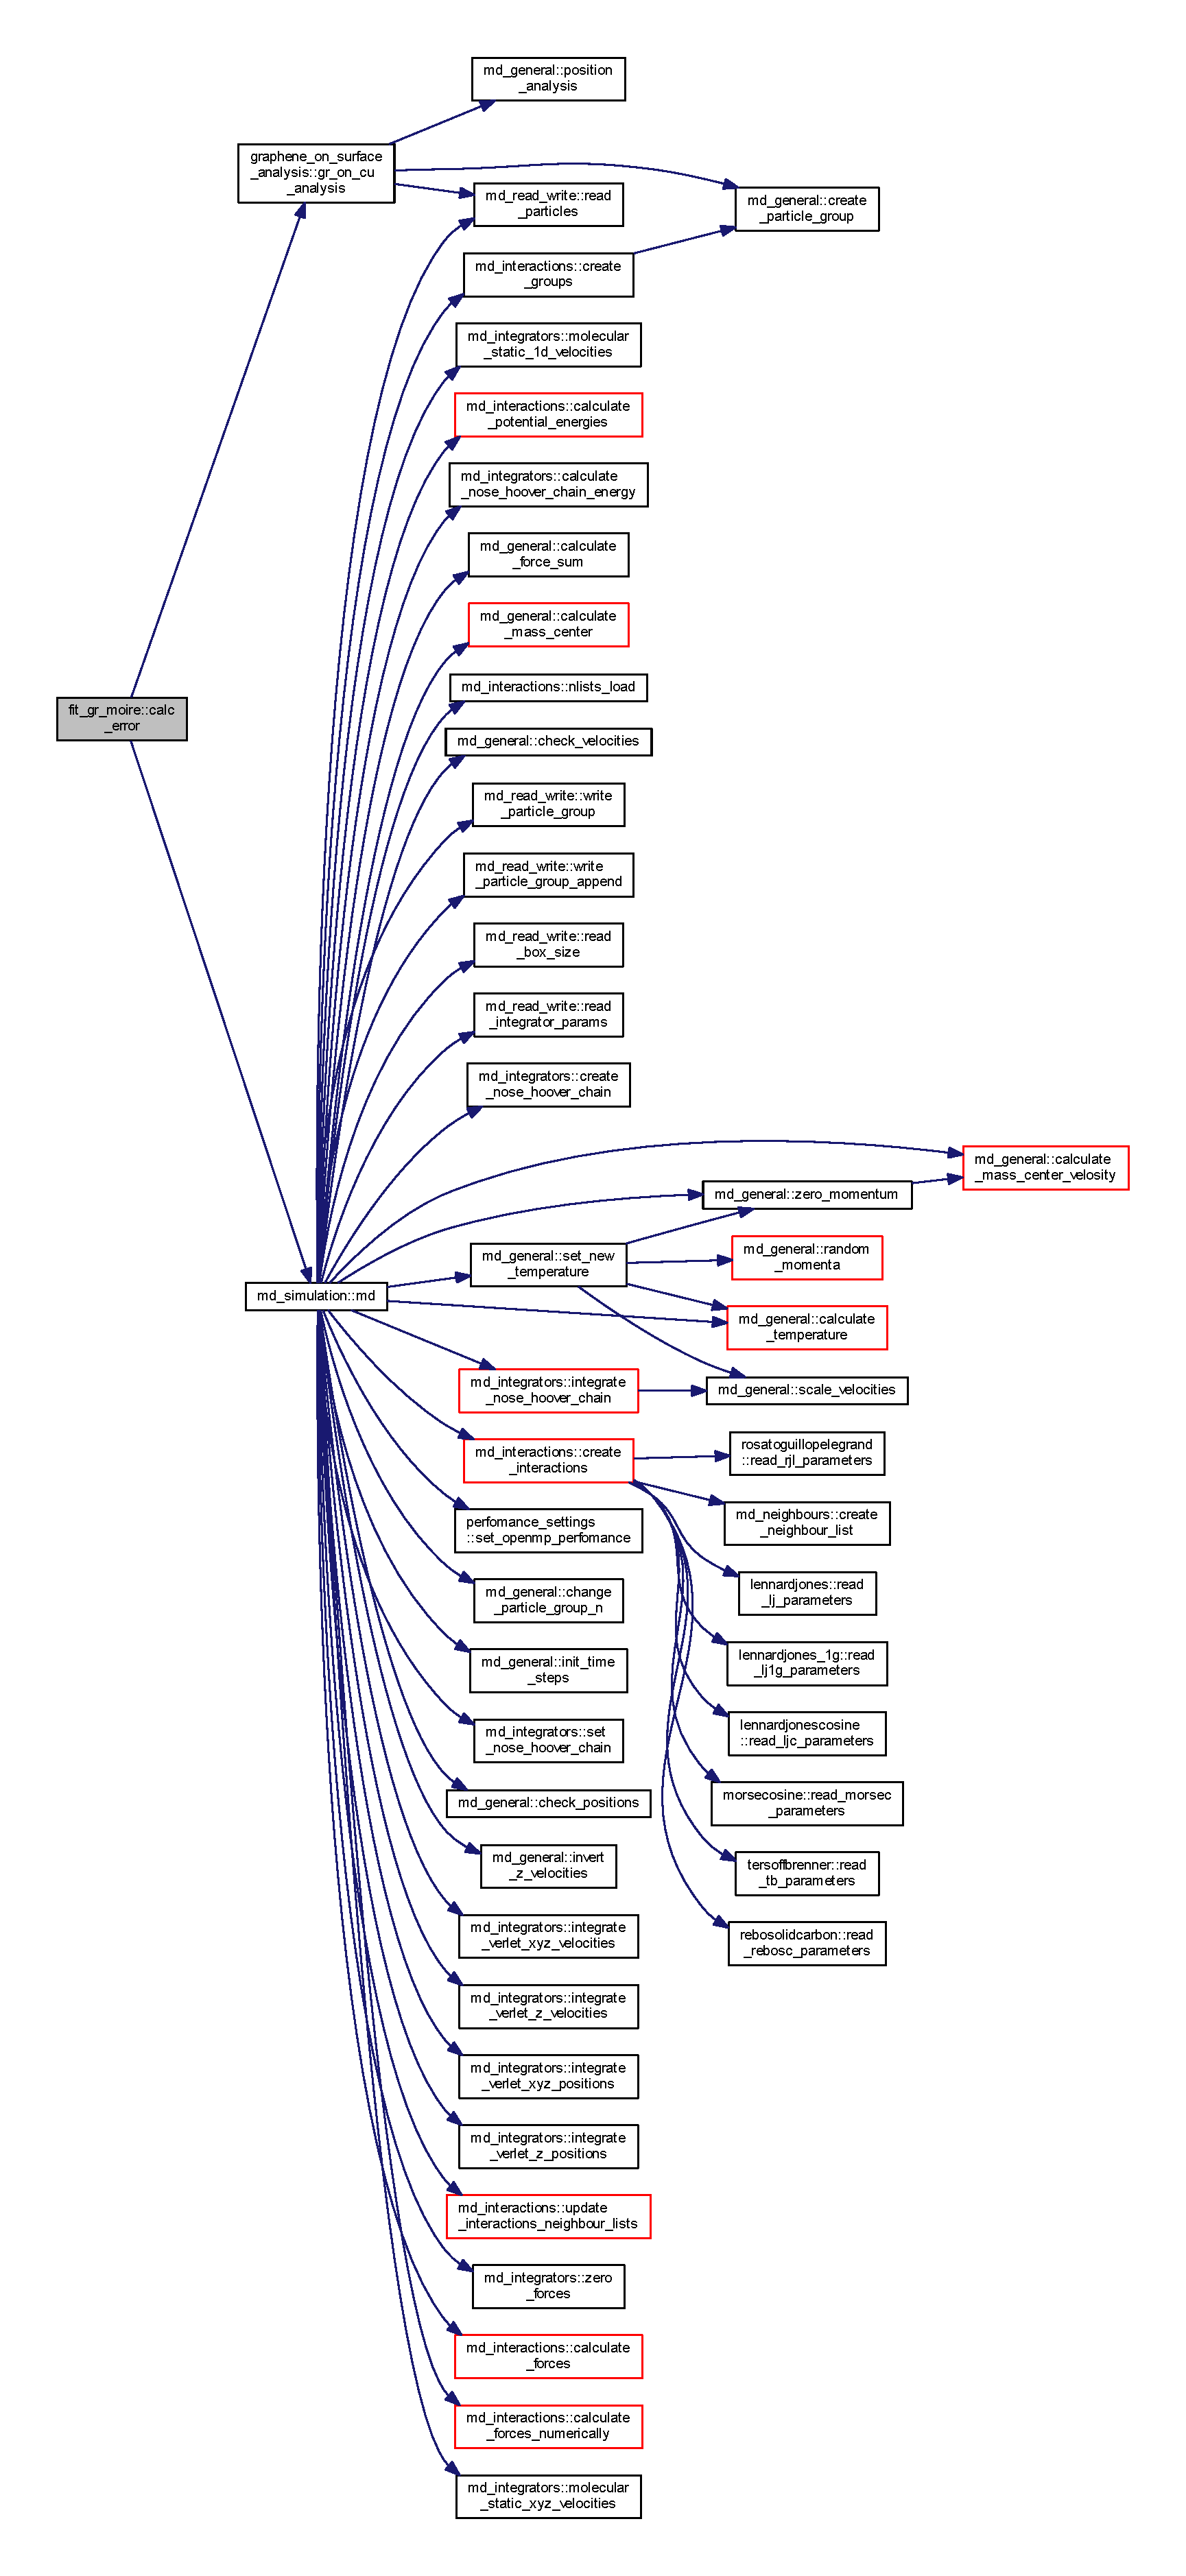
\includegraphics[height=550pt]{namespacefit__gr__moire_aafdddfaa3c2b90a3ab2c09735bc5068b_cgraph}
\end{center}
\end{figure}
\mbox{\Hypertarget{namespacefit__gr__moire_a68bd3fd9fb813f29fb1ba6ad58c05a9d}\label{namespacefit__gr__moire_a68bd3fd9fb813f29fb1ba6ad58c05a9d}} 
\index{fit\+\_\+gr\+\_\+moire@{fit\+\_\+gr\+\_\+moire}!set\+\_\+fitting\+\_\+parameters@{set\+\_\+fitting\+\_\+parameters}}
\index{set\+\_\+fitting\+\_\+parameters@{set\+\_\+fitting\+\_\+parameters}!fit\+\_\+gr\+\_\+moire@{fit\+\_\+gr\+\_\+moire}}
\subsubsection{\texorpdfstring{set\+\_\+fitting\+\_\+parameters()}{set\_fitting\_parameters()}}
{\footnotesize\ttfamily subroutine fit\+\_\+gr\+\_\+moire\+::set\+\_\+fitting\+\_\+parameters (\begin{DoxyParamCaption}\item[{character(len=256)}]{fitting\+\_\+parameters\+\_\+file\+\_\+name,  }\item[{real, dimension(4)}]{init\+\_\+min\+\_\+params,  }\item[{real, dimension(4)}]{init\+\_\+max\+\_\+params }\end{DoxyParamCaption})}



См. определение в файле fit\+\_\+gr\+\_\+moire.\+f90 строка 107


\begin{DoxyCode}
107 \textcolor{keywordtype}{real}                    :: init\_min\_params(4),init\_max\_params(4)
108 \textcolor{keywordtype}{character}(len=256)      :: fitting\_parameters\_file\_name,min\_param\_file,max\_param\_file,str
109 integer                 :: i
110 
111     final\_out\_id = 1211
112     oid = 111
113     \textcolor{keywordflow}{do} i=1,80
114         line(i:i) = \textcolor{stringliteral}{'\_'}
115 \textcolor{keywordflow}{    enddo}
116 
117     \textcolor{keyword}{open}(9,file=fitting\_parameters\_file\_name)
118     \textcolor{keyword}{read}(9,\textcolor{stringliteral}{'(A16,A)'}) str,input\_path;       \textcolor{keyword}{write}(out\_id,*) trim(str),\textcolor{stringliteral}{'  '},trim(input\_path)
119     \textcolor{keyword}{read}(9,\textcolor{stringliteral}{'(A16,A)'}) str,out\_path;         \textcolor{keyword}{write}(out\_id,*) trim(str),\textcolor{stringliteral}{'  '},trim(out\_path)
120     \textcolor{keyword}{read}(9,*) str,interaction\_name;         \textcolor{keyword}{write}(out\_id,*) trim(str),\textcolor{stringliteral}{'  '},trim(interaction\_name)
121     \textcolor{keyword}{read}(9,*) str,output\_prefix;            \textcolor{keyword}{write}(out\_id,*) trim(str),\textcolor{stringliteral}{'  '},trim(output\_prefix)
122     \textcolor{keyword}{read}(9,*) str,ar\_settings\_filename(1);  \textcolor{keyword}{write}(out\_id,*) trim(str),\textcolor{stringliteral}{'  '},trim(ar\_settings\_filename(1))
123     \textcolor{keyword}{read}(9,*) str,ar\_start\_xyz\_file(1);     \textcolor{keyword}{write}(out\_id,*) trim(str),\textcolor{stringliteral}{'  '},trim(ar\_start\_xyz\_file(1))
124     \textcolor{keyword}{read}(9,*) str,ar\_c\_num(1);              \textcolor{keyword}{write}(out\_id,*) trim(str),\textcolor{stringliteral}{'  '},ar\_c\_num(1)
125     \textcolor{keyword}{read}(9,*) str,ar\_zero\_energy\_level(1);  \textcolor{keyword}{write}(out\_id,*) trim(str),\textcolor{stringliteral}{'  '},ar\_zero\_energy\_level(1)
126     \textcolor{keyword}{read}(9,*) str,ar\_final\_file(1);         \textcolor{keyword}{write}(out\_id,*) trim(str),\textcolor{stringliteral}{'  '},trim(ar\_final\_file(1))
127     \textcolor{keyword}{read}(9,*) str,ar\_settings\_filename(2);  \textcolor{keyword}{write}(out\_id,*) trim(str),\textcolor{stringliteral}{'  '},trim(ar\_settings\_filename(2))
128     \textcolor{keyword}{read}(9,*) str,ar\_start\_xyz\_file(2);     \textcolor{keyword}{write}(out\_id,*) trim(str),\textcolor{stringliteral}{'  '},trim(ar\_start\_xyz\_file(2))
129     \textcolor{keyword}{read}(9,*) str,ar\_c\_num(2);              \textcolor{keyword}{write}(out\_id,*) trim(str),\textcolor{stringliteral}{'  '},ar\_c\_num(2)
130     \textcolor{keyword}{read}(9,*) str,ar\_zero\_energy\_level(2);  \textcolor{keyword}{write}(out\_id,*) trim(str),\textcolor{stringliteral}{'  '},ar\_zero\_energy\_level(2)
131     \textcolor{keyword}{read}(9,*) str,ar\_final\_file(2);         \textcolor{keyword}{write}(out\_id,*) trim(str),\textcolor{stringliteral}{'  '},trim(ar\_final\_file(2))
132     \textcolor{keyword}{read}(9,*) str,min\_param\_file;           \textcolor{keyword}{write}(out\_id,*) trim(str),\textcolor{stringliteral}{'  '},trim(min\_param\_file)
133     \textcolor{keyword}{read}(9,*) str,max\_param\_file;           \textcolor{keyword}{write}(out\_id,*) trim(str),\textcolor{stringliteral}{'  '},trim(max\_param\_file)
134     \textcolor{keyword}{read}(9,*) str,z;                        \textcolor{keyword}{write}(out\_id,*) trim(str),\textcolor{stringliteral}{'  '},z
135     \textcolor{keyword}{read}(9,*) str,be0;                      \textcolor{keyword}{write}(out\_id,*) trim(str),\textcolor{stringliteral}{'  '},be0
136     \textcolor{keyword}{read}(9,*) str,ar\_grd0(1);               \textcolor{keyword}{write}(out\_id,*) trim(str),\textcolor{stringliteral}{'  '},ar\_grd0(1)
137     \textcolor{keyword}{read}(9,*) str,ar\_grd0(2);               \textcolor{keyword}{write}(out\_id,*) trim(str),\textcolor{stringliteral}{'  '},ar\_grd0(2)
138     \textcolor{keyword}{close}(9)
139 
140 
141     simplified = .false.
142     \textcolor{keywordflow}{if}(interaction\_name==\textcolor{stringliteral}{'ljc'}) \textcolor{keywordflow}{then}
143         \textcolor{keyword}{open}(1234,file=trim(input\_path)//trim(min\_param\_file))
144         \textcolor{keyword}{read}(1234,*) init\_min\_params(3),init\_min\_params(1),init\_min\_params(2)
145         \textcolor{keyword}{read}(1234,*) rcut(1),rcut(2)
146         \textcolor{keyword}{close}(1234)
147         \textcolor{keyword}{open}(1234,file=trim(input\_path)//trim(max\_param\_file))
148         \textcolor{keyword}{read}(1234,*) init\_max\_params(3),init\_max\_params(1),init\_max\_params(2)
149         \textcolor{keyword}{close}(1234)
150         init\_min\_params(4) = 0.
151         init\_max\_params(4) = 0.
152 \textcolor{keywordflow}{    endif}
153     \textcolor{keywordflow}{if}(interaction\_name==\textcolor{stringliteral}{'morsec'}) \textcolor{keywordflow}{then}
154         \textcolor{keyword}{open}(1234,file=trim(input\_path)//trim(min\_param\_file))
155         \textcolor{keyword}{read}(1234,*) init\_min\_params(3),init\_min\_params(1),init\_min\_params(4),init\_min\_params(2)
156         \textcolor{keyword}{read}(1234,*) rcut(1),rcut(2)
157         \textcolor{keyword}{close}(1234)
158         \textcolor{keyword}{open}(1234,file=trim(input\_path)//trim(max\_param\_file))
159         \textcolor{keyword}{read}(1234,*) init\_max\_params(3),init\_max\_params(1),init\_max\_params(4),init\_max\_params(2)
160         \textcolor{keyword}{close}(1234)
161 \textcolor{keywordflow}{    endif}
162 
163     sim\_num = 0
164 
165     \textcolor{keyword}{open}(1234,file=trim(input\_path)//trim(ar\_settings\_filename(1)))
166     \textcolor{keyword}{read}(1234,*);\textcolor{keyword}{read}(1234,*);\textcolor{keyword}{read}(1234,*) str,ar\_xyz\_file(1)
167     \textcolor{keywordflow}{do} \textcolor{keywordflow}{while}(.true.)
168         \textcolor{keyword}{read}(1234,\textcolor{stringliteral}{'(A128)'}) str
169         \textcolor{keywordflow}{if}(str(1:3)==trim(interaction\_name)) \textcolor{keywordflow}{then}
170             \textcolor{keyword}{read}(str(4:),*) param\_file
171             \textcolor{keywordflow}{exit}
172 \textcolor{keywordflow}{        endif}
173         \textcolor{keywordflow}{if}(str(1:6)==trim(interaction\_name)) \textcolor{keywordflow}{then}
174             \textcolor{keyword}{read}(str(7:),*) param\_file
175             \textcolor{keywordflow}{exit}
176 \textcolor{keywordflow}{        endif}
177 \textcolor{keywordflow}{    enddo}
178     \textcolor{keyword}{close}(1234)
179     \textcolor{keyword}{open}(1234,file=trim(input\_path)//trim(ar\_settings\_filename(2)))
180     \textcolor{keyword}{read}(1234,*);\textcolor{keyword}{read}(1234,*);\textcolor{keyword}{read}(1234,*) str,ar\_xyz\_file(2)
181     \textcolor{keyword}{close}(1234)
182 
\end{DoxyCode}


\subsection{Переменные}
\mbox{\Hypertarget{namespacefit__gr__moire_abc1d82be5a435c0c119ec1d686f6771c}\label{namespacefit__gr__moire_abc1d82be5a435c0c119ec1d686f6771c}} 
\index{fit\+\_\+gr\+\_\+moire@{fit\+\_\+gr\+\_\+moire}!ar\+\_\+c\+\_\+num@{ar\+\_\+c\+\_\+num}}
\index{ar\+\_\+c\+\_\+num@{ar\+\_\+c\+\_\+num}!fit\+\_\+gr\+\_\+moire@{fit\+\_\+gr\+\_\+moire}}
\subsubsection{\texorpdfstring{ar\+\_\+c\+\_\+num}{ar\_c\_num}}
{\footnotesize\ttfamily integer, dimension(2) fit\+\_\+gr\+\_\+moire\+::ar\+\_\+c\+\_\+num}



См. определение в файле fit\+\_\+gr\+\_\+moire.\+f90 строка 7


\begin{DoxyCode}
7 integer                 :: ar\_c\_num(2)
\end{DoxyCode}
\mbox{\Hypertarget{namespacefit__gr__moire_a1e26c6ce1c81e9f34f2f2edd4fd40ae4}\label{namespacefit__gr__moire_a1e26c6ce1c81e9f34f2f2edd4fd40ae4}} 
\index{fit\+\_\+gr\+\_\+moire@{fit\+\_\+gr\+\_\+moire}!ar\+\_\+final\+\_\+file@{ar\+\_\+final\+\_\+file}}
\index{ar\+\_\+final\+\_\+file@{ar\+\_\+final\+\_\+file}!fit\+\_\+gr\+\_\+moire@{fit\+\_\+gr\+\_\+moire}}
\subsubsection{\texorpdfstring{ar\+\_\+final\+\_\+file}{ar\_final\_file}}
{\footnotesize\ttfamily character(len=256), dimension(2) fit\+\_\+gr\+\_\+moire\+::ar\+\_\+final\+\_\+file}



См. определение в файле fit\+\_\+gr\+\_\+moire.\+f90 строка 8

\mbox{\Hypertarget{namespacefit__gr__moire_a133d6649efb184d364f20a02e2afd05f}\label{namespacefit__gr__moire_a133d6649efb184d364f20a02e2afd05f}} 
\index{fit\+\_\+gr\+\_\+moire@{fit\+\_\+gr\+\_\+moire}!ar\+\_\+grd0@{ar\+\_\+grd0}}
\index{ar\+\_\+grd0@{ar\+\_\+grd0}!fit\+\_\+gr\+\_\+moire@{fit\+\_\+gr\+\_\+moire}}
\subsubsection{\texorpdfstring{ar\+\_\+grd0}{ar\_grd0}}
{\footnotesize\ttfamily real, dimension(2) fit\+\_\+gr\+\_\+moire\+::ar\+\_\+grd0}



См. определение в файле fit\+\_\+gr\+\_\+moire.\+f90 строка 10

\mbox{\Hypertarget{namespacefit__gr__moire_abe61efd3e06474bc596014a35475150c}\label{namespacefit__gr__moire_abe61efd3e06474bc596014a35475150c}} 
\index{fit\+\_\+gr\+\_\+moire@{fit\+\_\+gr\+\_\+moire}!ar\+\_\+settings\+\_\+filename@{ar\+\_\+settings\+\_\+filename}}
\index{ar\+\_\+settings\+\_\+filename@{ar\+\_\+settings\+\_\+filename}!fit\+\_\+gr\+\_\+moire@{fit\+\_\+gr\+\_\+moire}}
\subsubsection{\texorpdfstring{ar\+\_\+settings\+\_\+filename}{ar\_settings\_filename}}
{\footnotesize\ttfamily character(len=256), dimension(2) fit\+\_\+gr\+\_\+moire\+::ar\+\_\+settings\+\_\+filename}



См. определение в файле fit\+\_\+gr\+\_\+moire.\+f90 строка 8

\mbox{\Hypertarget{namespacefit__gr__moire_aa54f0200433f85f1399791f7128e94c5}\label{namespacefit__gr__moire_aa54f0200433f85f1399791f7128e94c5}} 
\index{fit\+\_\+gr\+\_\+moire@{fit\+\_\+gr\+\_\+moire}!ar\+\_\+start\+\_\+xyz\+\_\+file@{ar\+\_\+start\+\_\+xyz\+\_\+file}}
\index{ar\+\_\+start\+\_\+xyz\+\_\+file@{ar\+\_\+start\+\_\+xyz\+\_\+file}!fit\+\_\+gr\+\_\+moire@{fit\+\_\+gr\+\_\+moire}}
\subsubsection{\texorpdfstring{ar\+\_\+start\+\_\+xyz\+\_\+file}{ar\_start\_xyz\_file}}
{\footnotesize\ttfamily character(len=256), dimension(2) fit\+\_\+gr\+\_\+moire\+::ar\+\_\+start\+\_\+xyz\+\_\+file}



См. определение в файле fit\+\_\+gr\+\_\+moire.\+f90 строка 8

\mbox{\Hypertarget{namespacefit__gr__moire_adcea9b8af6d606b09d4cf11353d6e76a}\label{namespacefit__gr__moire_adcea9b8af6d606b09d4cf11353d6e76a}} 
\index{fit\+\_\+gr\+\_\+moire@{fit\+\_\+gr\+\_\+moire}!ar\+\_\+xyz\+\_\+file@{ar\+\_\+xyz\+\_\+file}}
\index{ar\+\_\+xyz\+\_\+file@{ar\+\_\+xyz\+\_\+file}!fit\+\_\+gr\+\_\+moire@{fit\+\_\+gr\+\_\+moire}}
\subsubsection{\texorpdfstring{ar\+\_\+xyz\+\_\+file}{ar\_xyz\_file}}
{\footnotesize\ttfamily character(len=256), dimension(2) fit\+\_\+gr\+\_\+moire\+::ar\+\_\+xyz\+\_\+file}



См. определение в файле fit\+\_\+gr\+\_\+moire.\+f90 строка 8

\mbox{\Hypertarget{namespacefit__gr__moire_a7b9059147432f1a2fab23cc7a14bda96}\label{namespacefit__gr__moire_a7b9059147432f1a2fab23cc7a14bda96}} 
\index{fit\+\_\+gr\+\_\+moire@{fit\+\_\+gr\+\_\+moire}!ar\+\_\+zero\+\_\+energy\+\_\+level@{ar\+\_\+zero\+\_\+energy\+\_\+level}}
\index{ar\+\_\+zero\+\_\+energy\+\_\+level@{ar\+\_\+zero\+\_\+energy\+\_\+level}!fit\+\_\+gr\+\_\+moire@{fit\+\_\+gr\+\_\+moire}}
\subsubsection{\texorpdfstring{ar\+\_\+zero\+\_\+energy\+\_\+level}{ar\_zero\_energy\_level}}
{\footnotesize\ttfamily real, dimension(2) fit\+\_\+gr\+\_\+moire\+::ar\+\_\+zero\+\_\+energy\+\_\+level}



См. определение в файле fit\+\_\+gr\+\_\+moire.\+f90 строка 10

\mbox{\Hypertarget{namespacefit__gr__moire_a9f35bc32182cc551fabbd2a3a172d812}\label{namespacefit__gr__moire_a9f35bc32182cc551fabbd2a3a172d812}} 
\index{fit\+\_\+gr\+\_\+moire@{fit\+\_\+gr\+\_\+moire}!be0@{be0}}
\index{be0@{be0}!fit\+\_\+gr\+\_\+moire@{fit\+\_\+gr\+\_\+moire}}
\subsubsection{\texorpdfstring{be0}{be0}}
{\footnotesize\ttfamily real fit\+\_\+gr\+\_\+moire\+::be0}



См. определение в файле fit\+\_\+gr\+\_\+moire.\+f90 строка 10

\mbox{\Hypertarget{namespacefit__gr__moire_a29fb26687189e2457138123a8a823147}\label{namespacefit__gr__moire_a29fb26687189e2457138123a8a823147}} 
\index{fit\+\_\+gr\+\_\+moire@{fit\+\_\+gr\+\_\+moire}!final\+\_\+out\+\_\+id@{final\+\_\+out\+\_\+id}}
\index{final\+\_\+out\+\_\+id@{final\+\_\+out\+\_\+id}!fit\+\_\+gr\+\_\+moire@{fit\+\_\+gr\+\_\+moire}}
\subsubsection{\texorpdfstring{final\+\_\+out\+\_\+id}{final\_out\_id}}
{\footnotesize\ttfamily integer fit\+\_\+gr\+\_\+moire\+::final\+\_\+out\+\_\+id}



См. определение в файле fit\+\_\+gr\+\_\+moire.\+f90 строка 6

\mbox{\Hypertarget{namespacefit__gr__moire_a5f4eb40eb6a559f446c1097c651da540}\label{namespacefit__gr__moire_a5f4eb40eb6a559f446c1097c651da540}} 
\index{fit\+\_\+gr\+\_\+moire@{fit\+\_\+gr\+\_\+moire}!input\+\_\+path@{input\+\_\+path}}
\index{input\+\_\+path@{input\+\_\+path}!fit\+\_\+gr\+\_\+moire@{fit\+\_\+gr\+\_\+moire}}
\subsubsection{\texorpdfstring{input\+\_\+path}{input\_path}}
{\footnotesize\ttfamily character(len=256) fit\+\_\+gr\+\_\+moire\+::input\+\_\+path}



См. определение в файле fit\+\_\+gr\+\_\+moire.\+f90 строка 8

\mbox{\Hypertarget{namespacefit__gr__moire_a7a35c12a582842134a9dac4018eddf7b}\label{namespacefit__gr__moire_a7a35c12a582842134a9dac4018eddf7b}} 
\index{fit\+\_\+gr\+\_\+moire@{fit\+\_\+gr\+\_\+moire}!interaction\+\_\+name@{interaction\+\_\+name}}
\index{interaction\+\_\+name@{interaction\+\_\+name}!fit\+\_\+gr\+\_\+moire@{fit\+\_\+gr\+\_\+moire}}
\subsubsection{\texorpdfstring{interaction\+\_\+name}{interaction\_name}}
{\footnotesize\ttfamily character(len=256) fit\+\_\+gr\+\_\+moire\+::interaction\+\_\+name}



См. определение в файле fit\+\_\+gr\+\_\+moire.\+f90 строка 8


\begin{DoxyCode}
8 \textcolor{comment}{character(len=256)      :: interaction\_name,ar\_settings\_filename(2),output\_prefix,input\_path,out\_path,&}
9                            ar\_final\_file(2),param\_file,ar\_start\_xyz\_file(2),ar\_xyz\_file(2)
\end{DoxyCode}
\mbox{\Hypertarget{namespacefit__gr__moire_a8fbbcfd1d9c1149a9182a782550ea455}\label{namespacefit__gr__moire_a8fbbcfd1d9c1149a9182a782550ea455}} 
\index{fit\+\_\+gr\+\_\+moire@{fit\+\_\+gr\+\_\+moire}!line@{line}}
\index{line@{line}!fit\+\_\+gr\+\_\+moire@{fit\+\_\+gr\+\_\+moire}}
\subsubsection{\texorpdfstring{line}{line}}
{\footnotesize\ttfamily character(len=80) fit\+\_\+gr\+\_\+moire\+::line}



См. определение в файле fit\+\_\+gr\+\_\+moire.\+f90 строка 12


\begin{DoxyCode}
12 \textcolor{comment}{character(len=80)       :: line}
\end{DoxyCode}
\mbox{\Hypertarget{namespacefit__gr__moire_a6b6dcf709ac2f8f7908b7d38fe795dcc}\label{namespacefit__gr__moire_a6b6dcf709ac2f8f7908b7d38fe795dcc}} 
\index{fit\+\_\+gr\+\_\+moire@{fit\+\_\+gr\+\_\+moire}!num\+\_\+of\+\_\+omp\+\_\+treads@{num\+\_\+of\+\_\+omp\+\_\+treads}}
\index{num\+\_\+of\+\_\+omp\+\_\+treads@{num\+\_\+of\+\_\+omp\+\_\+treads}!fit\+\_\+gr\+\_\+moire@{fit\+\_\+gr\+\_\+moire}}
\subsubsection{\texorpdfstring{num\+\_\+of\+\_\+omp\+\_\+treads}{num\_of\_omp\_treads}}
{\footnotesize\ttfamily integer fit\+\_\+gr\+\_\+moire\+::num\+\_\+of\+\_\+omp\+\_\+treads}



См. определение в файле fit\+\_\+gr\+\_\+moire.\+f90 строка 6

\mbox{\Hypertarget{namespacefit__gr__moire_a813dce231711455b1086fcd6fd95c2a4}\label{namespacefit__gr__moire_a813dce231711455b1086fcd6fd95c2a4}} 
\index{fit\+\_\+gr\+\_\+moire@{fit\+\_\+gr\+\_\+moire}!oid@{oid}}
\index{oid@{oid}!fit\+\_\+gr\+\_\+moire@{fit\+\_\+gr\+\_\+moire}}
\subsubsection{\texorpdfstring{oid}{oid}}
{\footnotesize\ttfamily integer fit\+\_\+gr\+\_\+moire\+::oid}



См. определение в файле fit\+\_\+gr\+\_\+moire.\+f90 строка 6

\mbox{\Hypertarget{namespacefit__gr__moire_a877e34e1da1ed0d899e33ed675b1f0e5}\label{namespacefit__gr__moire_a877e34e1da1ed0d899e33ed675b1f0e5}} 
\index{fit\+\_\+gr\+\_\+moire@{fit\+\_\+gr\+\_\+moire}!out\+\_\+id@{out\+\_\+id}}
\index{out\+\_\+id@{out\+\_\+id}!fit\+\_\+gr\+\_\+moire@{fit\+\_\+gr\+\_\+moire}}
\subsubsection{\texorpdfstring{out\+\_\+id}{out\_id}}
{\footnotesize\ttfamily integer fit\+\_\+gr\+\_\+moire\+::out\+\_\+id}



См. определение в файле fit\+\_\+gr\+\_\+moire.\+f90 строка 6

\mbox{\Hypertarget{namespacefit__gr__moire_a77444985e23a0fc091f7623c2c4469b3}\label{namespacefit__gr__moire_a77444985e23a0fc091f7623c2c4469b3}} 
\index{fit\+\_\+gr\+\_\+moire@{fit\+\_\+gr\+\_\+moire}!out\+\_\+path@{out\+\_\+path}}
\index{out\+\_\+path@{out\+\_\+path}!fit\+\_\+gr\+\_\+moire@{fit\+\_\+gr\+\_\+moire}}
\subsubsection{\texorpdfstring{out\+\_\+path}{out\_path}}
{\footnotesize\ttfamily character(len=256) fit\+\_\+gr\+\_\+moire\+::out\+\_\+path}



См. определение в файле fit\+\_\+gr\+\_\+moire.\+f90 строка 8

\mbox{\Hypertarget{namespacefit__gr__moire_a4a36513ac075c468e3f2c09114102f9b}\label{namespacefit__gr__moire_a4a36513ac075c468e3f2c09114102f9b}} 
\index{fit\+\_\+gr\+\_\+moire@{fit\+\_\+gr\+\_\+moire}!out\+\_\+period@{out\+\_\+period}}
\index{out\+\_\+period@{out\+\_\+period}!fit\+\_\+gr\+\_\+moire@{fit\+\_\+gr\+\_\+moire}}
\subsubsection{\texorpdfstring{out\+\_\+period}{out\_period}}
{\footnotesize\ttfamily integer fit\+\_\+gr\+\_\+moire\+::out\+\_\+period}



См. определение в файле fit\+\_\+gr\+\_\+moire.\+f90 строка 6

\mbox{\Hypertarget{namespacefit__gr__moire_ac107a23a93efd6c7247949001b635744}\label{namespacefit__gr__moire_ac107a23a93efd6c7247949001b635744}} 
\index{fit\+\_\+gr\+\_\+moire@{fit\+\_\+gr\+\_\+moire}!output\+\_\+prefix@{output\+\_\+prefix}}
\index{output\+\_\+prefix@{output\+\_\+prefix}!fit\+\_\+gr\+\_\+moire@{fit\+\_\+gr\+\_\+moire}}
\subsubsection{\texorpdfstring{output\+\_\+prefix}{output\_prefix}}
{\footnotesize\ttfamily character(len=256) fit\+\_\+gr\+\_\+moire\+::output\+\_\+prefix}



См. определение в файле fit\+\_\+gr\+\_\+moire.\+f90 строка 8

\mbox{\Hypertarget{namespacefit__gr__moire_a61b86e6a8a674b819bc9c8b166436c18}\label{namespacefit__gr__moire_a61b86e6a8a674b819bc9c8b166436c18}} 
\index{fit\+\_\+gr\+\_\+moire@{fit\+\_\+gr\+\_\+moire}!param\+\_\+file@{param\+\_\+file}}
\index{param\+\_\+file@{param\+\_\+file}!fit\+\_\+gr\+\_\+moire@{fit\+\_\+gr\+\_\+moire}}
\subsubsection{\texorpdfstring{param\+\_\+file}{param\_file}}
{\footnotesize\ttfamily character(len=256) fit\+\_\+gr\+\_\+moire\+::param\+\_\+file}



См. определение в файле fit\+\_\+gr\+\_\+moire.\+f90 строка 8

\mbox{\Hypertarget{namespacefit__gr__moire_aa4a0f3a112959e7b4ce4105b57b1ac8b}\label{namespacefit__gr__moire_aa4a0f3a112959e7b4ce4105b57b1ac8b}} 
\index{fit\+\_\+gr\+\_\+moire@{fit\+\_\+gr\+\_\+moire}!rcut@{rcut}}
\index{rcut@{rcut}!fit\+\_\+gr\+\_\+moire@{fit\+\_\+gr\+\_\+moire}}
\subsubsection{\texorpdfstring{rcut}{rcut}}
{\footnotesize\ttfamily real, dimension(2) fit\+\_\+gr\+\_\+moire\+::rcut}



См. определение в файле fit\+\_\+gr\+\_\+moire.\+f90 строка 10

\mbox{\Hypertarget{namespacefit__gr__moire_aace6796e23a47584768373466a2a7522}\label{namespacefit__gr__moire_aace6796e23a47584768373466a2a7522}} 
\index{fit\+\_\+gr\+\_\+moire@{fit\+\_\+gr\+\_\+moire}!sim\+\_\+num@{sim\+\_\+num}}
\index{sim\+\_\+num@{sim\+\_\+num}!fit\+\_\+gr\+\_\+moire@{fit\+\_\+gr\+\_\+moire}}
\subsubsection{\texorpdfstring{sim\+\_\+num}{sim\_num}}
{\footnotesize\ttfamily integer fit\+\_\+gr\+\_\+moire\+::sim\+\_\+num}



См. определение в файле fit\+\_\+gr\+\_\+moire.\+f90 строка 6


\begin{DoxyCode}
6 integer                 :: sim\_num,out\_period,num\_of\_omp\_treads,out\_id,final\_out\_id,oid
\end{DoxyCode}
\mbox{\Hypertarget{namespacefit__gr__moire_a9092ed380be5233a800406322be81218}\label{namespacefit__gr__moire_a9092ed380be5233a800406322be81218}} 
\index{fit\+\_\+gr\+\_\+moire@{fit\+\_\+gr\+\_\+moire}!simplified@{simplified}}
\index{simplified@{simplified}!fit\+\_\+gr\+\_\+moire@{fit\+\_\+gr\+\_\+moire}}
\subsubsection{\texorpdfstring{simplified}{simplified}}
{\footnotesize\ttfamily logical fit\+\_\+gr\+\_\+moire\+::simplified}



См. определение в файле fit\+\_\+gr\+\_\+moire.\+f90 строка 11


\begin{DoxyCode}
11 logical                 :: simplified
\end{DoxyCode}
\mbox{\Hypertarget{namespacefit__gr__moire_ad1616f835d2564c00ebea11a9c88cbaf}\label{namespacefit__gr__moire_ad1616f835d2564c00ebea11a9c88cbaf}} 
\index{fit\+\_\+gr\+\_\+moire@{fit\+\_\+gr\+\_\+moire}!z@{z}}
\index{z@{z}!fit\+\_\+gr\+\_\+moire@{fit\+\_\+gr\+\_\+moire}}
\subsubsection{\texorpdfstring{z}{z}}
{\footnotesize\ttfamily real fit\+\_\+gr\+\_\+moire\+::z}



См. определение в файле fit\+\_\+gr\+\_\+moire.\+f90 строка 10


\begin{DoxyCode}
10 \textcolor{keywordtype}{real}                    :: z,ar\_zero\_energy\_level(2),be0,ar\_grd0(2),Rcut(2)
\end{DoxyCode}

\hypertarget{namespacegraphene__on__surface__analysis}{}\section{Модуль graphene\+\_\+on\+\_\+surface\+\_\+analysis}
\label{namespacegraphene__on__surface__analysis}\index{graphene\+\_\+on\+\_\+surface\+\_\+analysis@{graphene\+\_\+on\+\_\+surface\+\_\+analysis}}
\subsection*{Функции/подпрограммы}
\begin{DoxyCompactItemize}
\item 
subroutine \mbox{\hyperlink{namespacegraphene__on__surface__analysis_a02cffcc8904565bfaf36c4503f30f759}{gr\+\_\+on\+\_\+cu\+\_\+analysis}} (arr1, arr2, filename, z)
\end{DoxyCompactItemize}


\subsection{Функции/подпрограммы}
\mbox{\Hypertarget{namespacegraphene__on__surface__analysis_a02cffcc8904565bfaf36c4503f30f759}\label{namespacegraphene__on__surface__analysis_a02cffcc8904565bfaf36c4503f30f759}} 
\index{graphene\+\_\+on\+\_\+surface\+\_\+analysis@{graphene\+\_\+on\+\_\+surface\+\_\+analysis}!gr\+\_\+on\+\_\+cu\+\_\+analysis@{gr\+\_\+on\+\_\+cu\+\_\+analysis}}
\index{gr\+\_\+on\+\_\+cu\+\_\+analysis@{gr\+\_\+on\+\_\+cu\+\_\+analysis}!graphene\+\_\+on\+\_\+surface\+\_\+analysis@{graphene\+\_\+on\+\_\+surface\+\_\+analysis}}
\subsubsection{\texorpdfstring{gr\+\_\+on\+\_\+cu\+\_\+analysis()}{gr\_on\_cu\_analysis()}}
{\footnotesize\ttfamily subroutine graphene\+\_\+on\+\_\+surface\+\_\+analysis\+::gr\+\_\+on\+\_\+cu\+\_\+analysis (\begin{DoxyParamCaption}\item[{real, dimension(3)}]{arr1,  }\item[{real, dimension(3)}]{arr2,  }\item[{character(len=256)}]{filename,  }\item[{real}]{z }\end{DoxyParamCaption})}



См. определение в файле graphene\+\_\+on\+\_\+surface\+\_\+analysis.\+f90 строка 9


\begin{DoxyCode}
9     \textcolor{keywordtype}{type}(particles)                         :: atoms
10     \textcolor{keywordtype}{type}(particle\_group)                    :: groupC,groupCU
11     \textcolor{keywordtype}{character}(len=256)                      :: filename
12     \textcolor{keywordtype}{character}(len=32)                       :: type\_names(3)
13     real                                    :: z,arr1(3),arr2(3)
14 
15     \textcolor{keyword}{call }read\_particles(atoms,filename)
16     type\_names(1) = \textcolor{stringliteral}{'C'};    type\_names(2) = \textcolor{stringliteral}{'C\_a'};      type\_names(3) = \textcolor{stringliteral}{'C\_b'}
17     \textcolor{keyword}{call }create\_particle\_group(groupc,type\_names,atoms)
18     \textcolor{keyword}{call }position\_analysis(arr1(1),arr1(2),arr1(3),atoms,groupc,3,z,1000.)
19     type\_names(1) = \textcolor{stringliteral}{'CU'};   type\_names(2) = \textcolor{stringliteral}{'CU\_fixed'}; type\_names(3) = \textcolor{stringliteral}{'#'}
20     \textcolor{keyword}{call }create\_particle\_group(groupcu,type\_names,atoms)
21     \textcolor{keyword}{call }position\_analysis(arr2(1),arr2(2),arr2(3),atoms,groupcu,3,z,1000.)
22     \textcolor{keyword}{deallocate}(atoms%positions)
23     \textcolor{keyword}{deallocate}(atoms%velocities)
24     \textcolor{keyword}{deallocate}(atoms%forces)
25     \textcolor{keyword}{deallocate}(atoms%masses)
26     \textcolor{keyword}{deallocate}(atoms%atom\_types)
27     \textcolor{keyword}{deallocate}(groupc%indexes)
28     \textcolor{keyword}{deallocate}(groupcu%indexes)
29     
\end{DoxyCode}
Граф вызовов\+:\nopagebreak
\begin{figure}[H]
\begin{center}
\leavevmode
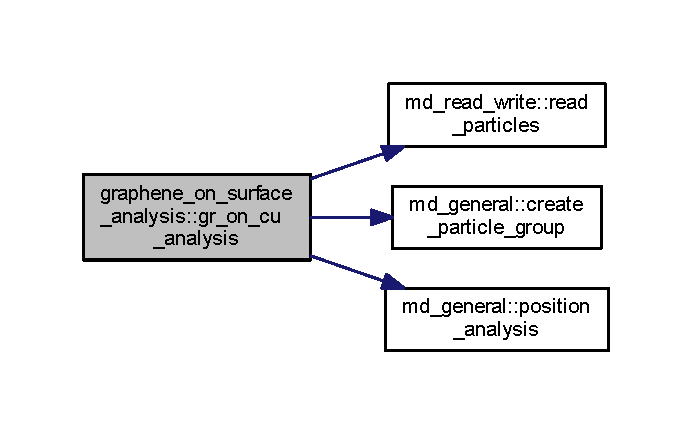
\includegraphics[width=332pt]{namespacegraphene__on__surface__analysis_a02cffcc8904565bfaf36c4503f30f759_cgraph}
\end{center}
\end{figure}

\hypertarget{namespacegraphenenorm}{}\section{Модуль graphenenorm}
\label{namespacegraphenenorm}\index{graphenenorm@{graphenenorm}}
\subsection*{Функции/подпрограммы}
\begin{DoxyCompactItemize}
\item 
subroutine \mbox{\hyperlink{namespacegraphenenorm_afb5708c33c6fe9d316e999710adeeef5}{find\+\_\+gr\+\_\+nearest\+\_\+neighbors}} (nl\+\_\+nn, nl)
\item 
subroutine \mbox{\hyperlink{namespacegraphenenorm_a6005cfed33b7112df95442616a990b5b}{find\+\_\+norm\+\_\+in\+\_\+graphene}} (gr\+\_\+norm, dr\+\_\+nn)
\item 
subroutine \mbox{\hyperlink{namespacegraphenenorm_a16d22fddd4c9f90cdf1236130515fd24}{update\+\_\+nearest\+\_\+neighbours\+\_\+in\+\_\+graphene}} (md\+\_\+step, nl\+\_\+nn, nl, atoms, group, box)
\end{DoxyCompactItemize}


\subsection{Функции/подпрограммы}
\mbox{\Hypertarget{namespacegraphenenorm_afb5708c33c6fe9d316e999710adeeef5}\label{namespacegraphenenorm_afb5708c33c6fe9d316e999710adeeef5}} 
\index{graphenenorm@{graphenenorm}!find\+\_\+gr\+\_\+nearest\+\_\+neighbors@{find\+\_\+gr\+\_\+nearest\+\_\+neighbors}}
\index{find\+\_\+gr\+\_\+nearest\+\_\+neighbors@{find\+\_\+gr\+\_\+nearest\+\_\+neighbors}!graphenenorm@{graphenenorm}}
\subsubsection{\texorpdfstring{find\+\_\+gr\+\_\+nearest\+\_\+neighbors()}{find\_gr\_nearest\_neighbors()}}
{\footnotesize\ttfamily subroutine graphenenorm\+::find\+\_\+gr\+\_\+nearest\+\_\+neighbors (\begin{DoxyParamCaption}\item[{type(\mbox{\hyperlink{structmd__general_1_1neighbour__list}{neighbour\+\_\+list}})}]{nl\+\_\+nn,  }\item[{type(\mbox{\hyperlink{structmd__general_1_1neighbour__list}{neighbour\+\_\+list}})}]{nl }\end{DoxyParamCaption})}



См. определение в файле graphenenorm.\+f90 строка 9


\begin{DoxyCode}
9     \textcolor{keywordtype}{type}(neighbour\_list):: nl,nl\_nn
10     \textcolor{keywordtype}{integer}:: nnum\_nn,i,p,k 
11     
12     nnum\_nn = 3
13     \textcolor{keywordflow}{if}(nl\_nn%neighb\_num\_max/=nnum\_nn) then; \textcolor{keyword}{write}(*,*) \textcolor{stringliteral}{'error: nl\_nn%neighb\_num\_max/=nnum\_nn'}; stop;\textcolor{keywordflow}{ endif}
14     \textcolor{comment}{!$OMP PARALLEL firstprivate(i,p,k)}
15     \textcolor{comment}{!$OMP DO}
16     \textcolor{keywordflow}{do} i=1,nl%N
17         k = 0
18         \textcolor{keywordflow}{do} p=1,nl%nnum(i)
19             \textcolor{keywordflow}{if} (nl%moddr(p,i)<nl\_nn%r\_cut) \textcolor{keywordflow}{then}
20                 k = k+1
21                 \textcolor{keywordflow}{if} (k<=nnum\_nn) \textcolor{keywordflow}{then}
22                     nl\_nn%nlist(k,i) = nl%nlist(p,i)
23                     nl\_nn%moddr(k,i) = nl%moddr(p,i)
24                     nl\_nn%dr(:,k,i) = nl%dr(:,p,i)
25                 \textcolor{keywordflow}{else}
26                     \textcolor{keyword}{write}(*,*) \textcolor{stringliteral}{'error: too many gr nearest neibs'},i,p,nl%moddr(p,i); stop;
27 \textcolor{keywordflow}{                endif}
28 \textcolor{keywordflow}{            endif}
29 \textcolor{keywordflow}{        enddo}
30         \textcolor{keywordflow}{if} (k/=nnum\_nn) then; \textcolor{keyword}{write}(*,*) \textcolor{stringliteral}{'error: not enough gr nearest neibs'},i,nl\_nn%moddr(:,i),nl\_nn
      %nlist(:,i); stop; endif;
31         nl\_nn%nnum(i) = nnum\_nn
32 \textcolor{keywordflow}{    enddo}
33     \textcolor{comment}{!$OMP END DO}
34     \textcolor{comment}{!$OMP END PARALLEL}
35     
\end{DoxyCode}
\mbox{\Hypertarget{namespacegraphenenorm_a6005cfed33b7112df95442616a990b5b}\label{namespacegraphenenorm_a6005cfed33b7112df95442616a990b5b}} 
\index{graphenenorm@{graphenenorm}!find\+\_\+norm\+\_\+in\+\_\+graphene@{find\+\_\+norm\+\_\+in\+\_\+graphene}}
\index{find\+\_\+norm\+\_\+in\+\_\+graphene@{find\+\_\+norm\+\_\+in\+\_\+graphene}!graphenenorm@{graphenenorm}}
\subsubsection{\texorpdfstring{find\+\_\+norm\+\_\+in\+\_\+graphene()}{find\_norm\_in\_graphene()}}
{\footnotesize\ttfamily subroutine graphenenorm\+::find\+\_\+norm\+\_\+in\+\_\+graphene (\begin{DoxyParamCaption}\item[{real, dimension(\+:,\+:)}]{gr\+\_\+norm,  }\item[{real, dimension(\+:,\+:,\+:)}]{dr\+\_\+nn }\end{DoxyParamCaption})}



См. определение в файле graphenenorm.\+f90 строка 39


\begin{DoxyCode}
39     \textcolor{keywordtype}{integer}:: nnum\_nn,i,p,k
40     \textcolor{keywordtype}{real}:: dr\_nn(:,:,:),gr\_norm(:,:),drj12(3),drj31(3)
41     
42     nnum\_nn = 3
43     \textcolor{comment}{!$OMP PARALLEL firstprivate(i,p,k,drj12,drj31)}
44     \textcolor{comment}{!$OMP DO}
45     \textcolor{keywordflow}{do} i=1,\textcolor{keyword}{size}(gr\_norm(1,:))
46         drj12 = dr\_nn(:,2,i)-dr\_nn(:,1,i)
47         drj31 = dr\_nn(:,1,i)-dr\_nn(:,3,i)
48         \textcolor{keywordflow}{do} k=1,3
49             gr\_norm(k,i) = (drj12(mod(k,3)+1))*(drj31(mod(k+1,3)+1))-(drj12(mod(k+1,3)+1))*(drj31(mod(k,3)+
      1))
50 \textcolor{keywordflow}{        enddo}
51         \textcolor{keywordflow}{if} (gr\_norm(3,i)<0.) gr\_norm(:,i)=-gr\_norm(:,i)
52         gr\_norm(:,i) = gr\_norm(:,i)/sqrt(sum(gr\_norm(:,i)**2))
53 \textcolor{keywordflow}{    enddo}
54     \textcolor{comment}{!$OMP END DO}
55     \textcolor{comment}{!$OMP END PARALLEL  }
\end{DoxyCode}
\mbox{\Hypertarget{namespacegraphenenorm_a16d22fddd4c9f90cdf1236130515fd24}\label{namespacegraphenenorm_a16d22fddd4c9f90cdf1236130515fd24}} 
\index{graphenenorm@{graphenenorm}!update\+\_\+nearest\+\_\+neighbours\+\_\+in\+\_\+graphene@{update\+\_\+nearest\+\_\+neighbours\+\_\+in\+\_\+graphene}}
\index{update\+\_\+nearest\+\_\+neighbours\+\_\+in\+\_\+graphene@{update\+\_\+nearest\+\_\+neighbours\+\_\+in\+\_\+graphene}!graphenenorm@{graphenenorm}}
\subsubsection{\texorpdfstring{update\+\_\+nearest\+\_\+neighbours\+\_\+in\+\_\+graphene()}{update\_nearest\_neighbours\_in\_graphene()}}
{\footnotesize\ttfamily subroutine graphenenorm\+::update\+\_\+nearest\+\_\+neighbours\+\_\+in\+\_\+graphene (\begin{DoxyParamCaption}\item[{integer}]{md\+\_\+step,  }\item[{type(\mbox{\hyperlink{structmd__general_1_1neighbour__list}{neighbour\+\_\+list}})}]{nl\+\_\+nn,  }\item[{type(\mbox{\hyperlink{structmd__general_1_1neighbour__list}{neighbour\+\_\+list}})}]{nl,  }\item[{type(\mbox{\hyperlink{structmd__general_1_1particles}{particles}})}]{atoms,  }\item[{type(\mbox{\hyperlink{structmd__general_1_1particle__group}{particle\+\_\+group}})}]{group,  }\item[{type(\mbox{\hyperlink{structmd__general_1_1simulation__cell}{simulation\+\_\+cell}})}]{box }\end{DoxyParamCaption})}



См. определение в файле graphenenorm.\+f90 строка 59


\begin{DoxyCode}
59     \textcolor{keywordtype}{type}(particles)::   atoms
60     \textcolor{keywordtype}{type}(neighbour\_list):: nl,nl\_nn
61     \textcolor{keywordtype}{type}(particle\_group):: group
62     \textcolor{keywordtype}{type}(simulation\_cell):: box
63     \textcolor{keywordtype}{integer}:: md\_step
64 
65     \textcolor{keywordflow}{if} (mod(md\_step,nl%update\_period)==0) \textcolor{keywordflow}{then}
66         \textcolor{keyword}{call }find\_gr\_nearest\_neighbors(nl\_nn,nl)
67     \textcolor{keywordflow}{else}
68         \textcolor{keyword}{call }find\_neighbour\_distances(nl\_nn,atoms,group,group,box)
69 \textcolor{keywordflow}{    endif}
70     
\end{DoxyCode}
Граф вызовов\+:\nopagebreak
\begin{figure}[H]
\begin{center}
\leavevmode
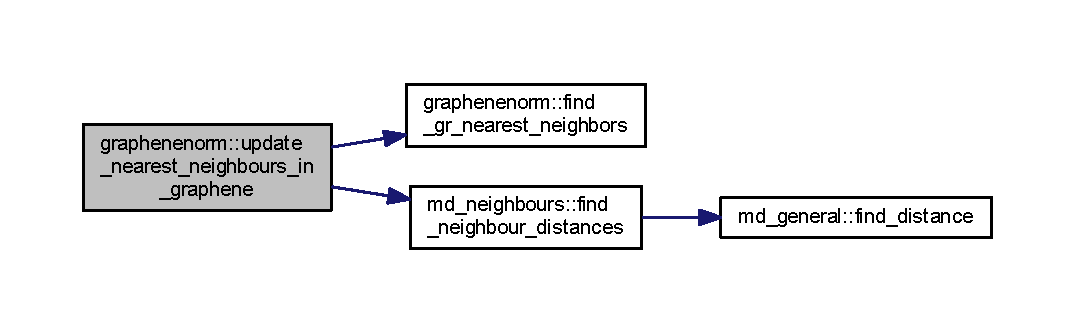
\includegraphics[width=350pt]{namespacegraphenenorm_a16d22fddd4c9f90cdf1236130515fd24_cgraph}
\end{center}
\end{figure}

\hypertarget{namespaceifport}{}\section{Модуль ifport}
\label{namespaceifport}\index{ifport@{ifport}}


Заглушка для удобства компиляции.  В I\+F\+P\+O\+RT находится функция rand() при компиляции с ifort. При компиляции с gfortran такого модуля нет. Этот пустой модуль нужен чтобы не убирать use I\+F\+P\+O\+RT в \mbox{\hyperlink{namespacemd__general}{md\+\_\+general}} при компиляции с gfortran.  




\subsection{Подробное описание}
Заглушка для удобства компиляции.  В I\+F\+P\+O\+RT находится функция rand() при компиляции с ifort. При компиляции с gfortran такого модуля нет. Этот пустой модуль нужен чтобы не убирать use I\+F\+P\+O\+RT в \mbox{\hyperlink{namespacemd__general}{md\+\_\+general}} при компиляции с gfortran. 
\hypertarget{namespacelennardjones}{}\section{Модуль lennardjones}
\label{namespacelennardjones}\index{lennardjones@{lennardjones}}
\subsection*{Типы данных}
\begin{DoxyCompactItemize}
\item 
type \mbox{\hyperlink{structlennardjones_1_1lennardjones__parameters}{lennardjones\+\_\+parameters}}
\end{DoxyCompactItemize}
\subsection*{Функции/подпрограммы}
\begin{DoxyCompactItemize}
\item 
subroutine \mbox{\hyperlink{namespacelennardjones_ace8630f2bebc2a2aac8ab12a64aedffa}{read\+\_\+lj\+\_\+parameters}} (L\+Jp, filename)
\item 
subroutine \mbox{\hyperlink{namespacelennardjones_af8b565355907ac9a41a6336acd884a37}{lj\+\_\+energy}} (energy, nl, L\+Jp)
\item 
subroutine \mbox{\hyperlink{namespacelennardjones_af88358c174f20878507192477e6b8dde}{lj\+\_\+forces}} (atoms, nl, L\+Jp)
\end{DoxyCompactItemize}


\subsection{Функции/подпрограммы}
\mbox{\Hypertarget{namespacelennardjones_af8b565355907ac9a41a6336acd884a37}\label{namespacelennardjones_af8b565355907ac9a41a6336acd884a37}} 
\index{lennardjones@{lennardjones}!lj\+\_\+energy@{lj\+\_\+energy}}
\index{lj\+\_\+energy@{lj\+\_\+energy}!lennardjones@{lennardjones}}
\subsubsection{\texorpdfstring{lj\+\_\+energy()}{lj\_energy()}}
{\footnotesize\ttfamily subroutine lennardjones\+::lj\+\_\+energy (\begin{DoxyParamCaption}\item[{real}]{energy,  }\item[{type(\mbox{\hyperlink{structmd__general_1_1neighbour__list}{neighbour\+\_\+list}})}]{nl,  }\item[{type(\mbox{\hyperlink{structlennardjones_1_1lennardjones__parameters}{lennardjones\+\_\+parameters}})}]{L\+Jp }\end{DoxyParamCaption})}



См. определение в файле Lennard\+Jones.\+f90 строка 24


\begin{DoxyCode}
24     \textcolor{keywordtype}{type}(neighbour\_list):: nl
25     \textcolor{keywordtype}{type}(LennardJones\_parameters):: LJp
26     \textcolor{keywordtype}{integer}:: i,p
27     \textcolor{keywordtype}{real}:: energy,energy\_priv,V
28     
29     energy = 0.
30     energy\_priv = 0.
31     \textcolor{comment}{!$OMP PARALLEL firstprivate(energy\_priv,i,p,V)}
32     \textcolor{comment}{!$OMP DO}
33     \textcolor{keywordflow}{do} i=1,nl%N
34         \textcolor{keywordflow}{do} p=1,nl%nnum(i)
35             \textcolor{keywordflow}{if} (nl%moddr(p,i)<ljp%R2) \textcolor{keywordflow}{then}
36                 v = (ljp%sig/nl%moddr(p,i))**6
37                 energy\_priv = energy\_priv+4*ljp%eps*v*(v-1.)*f\_cut(nl%moddr(p,i),ljp%R1,ljp%R2)
38 \textcolor{keywordflow}{            endif}   
39 \textcolor{keywordflow}{        enddo}
40 \textcolor{keywordflow}{    enddo}
41     \textcolor{comment}{!$OMP END DO}
42     \textcolor{comment}{!$OMP ATOMIC}
43         energy = energy+energy\_priv
44     \textcolor{comment}{!$OMP END PARALLEL}
45     
\end{DoxyCode}
Граф вызовов\+:\nopagebreak
\begin{figure}[H]
\begin{center}
\leavevmode
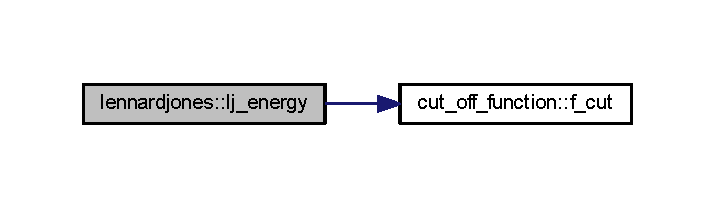
\includegraphics[width=343pt]{namespacelennardjones_af8b565355907ac9a41a6336acd884a37_cgraph}
\end{center}
\end{figure}
\mbox{\Hypertarget{namespacelennardjones_af88358c174f20878507192477e6b8dde}\label{namespacelennardjones_af88358c174f20878507192477e6b8dde}} 
\index{lennardjones@{lennardjones}!lj\+\_\+forces@{lj\+\_\+forces}}
\index{lj\+\_\+forces@{lj\+\_\+forces}!lennardjones@{lennardjones}}
\subsubsection{\texorpdfstring{lj\+\_\+forces()}{lj\_forces()}}
{\footnotesize\ttfamily subroutine lennardjones\+::lj\+\_\+forces (\begin{DoxyParamCaption}\item[{type(\mbox{\hyperlink{structmd__general_1_1particles}{particles}})}]{atoms,  }\item[{type(\mbox{\hyperlink{structmd__general_1_1neighbour__list}{neighbour\+\_\+list}})}]{nl,  }\item[{type(\mbox{\hyperlink{structlennardjones_1_1lennardjones__parameters}{lennardjones\+\_\+parameters}})}]{L\+Jp }\end{DoxyParamCaption})}



См. определение в файле Lennard\+Jones.\+f90 строка 49


\begin{DoxyCode}
49     \textcolor{keywordtype}{type}(particles)::   atoms
50     \textcolor{keywordtype}{type}(neighbour\_list):: nl
51     \textcolor{keywordtype}{type}(LennardJones\_parameters):: LJp
52     \textcolor{keywordtype}{integer}:: i,p
53     \textcolor{keywordtype}{real}:: V
54     
55     \textcolor{comment}{!$OMP PARALLEL firstprivate(i,p,V)}
56     \textcolor{comment}{!$OMP DO}
57     \textcolor{keywordflow}{do} i=1,nl%N
58         \textcolor{keywordflow}{do} p=1,nl%nnum(i)
59             \textcolor{keywordflow}{if} (nl%moddr(p,i)<ljp%R2) \textcolor{keywordflow}{then}
60                 v = (ljp%sig/nl%moddr(p,i))**6
61                 atoms%forces(:,nl%particle\_index(i)) = atoms%forces(:,nl%particle\_index(i))-4.*ljp%eps*&
62                 (v*(12.*v-6.)/nl%moddr(p,i)**2*f\_cut(nl%moddr(p,i),ljp%R1,ljp%R2)-v*(v-1.)*df\_cut(nl%moddr(
      p,i),ljp%R1,ljp%R2))*nl%dr(:,p,i)
63 \textcolor{keywordflow}{            endif}
64 \textcolor{keywordflow}{        enddo}
65 \textcolor{keywordflow}{    enddo}
66     \textcolor{comment}{!$OMP END DO}
67     \textcolor{comment}{!$OMP END PARALLEL}
68     
\end{DoxyCode}
Граф вызовов\+:\nopagebreak
\begin{figure}[H]
\begin{center}
\leavevmode
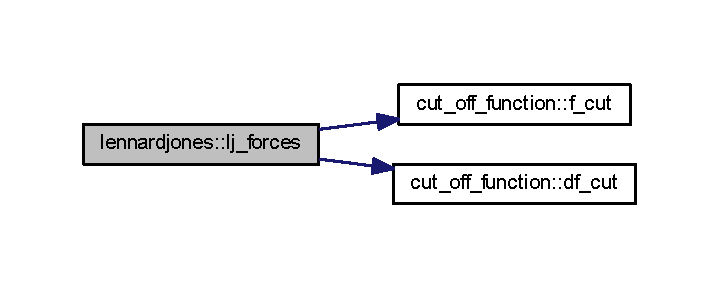
\includegraphics[width=345pt]{namespacelennardjones_af88358c174f20878507192477e6b8dde_cgraph}
\end{center}
\end{figure}
\mbox{\Hypertarget{namespacelennardjones_ace8630f2bebc2a2aac8ab12a64aedffa}\label{namespacelennardjones_ace8630f2bebc2a2aac8ab12a64aedffa}} 
\index{lennardjones@{lennardjones}!read\+\_\+lj\+\_\+parameters@{read\+\_\+lj\+\_\+parameters}}
\index{read\+\_\+lj\+\_\+parameters@{read\+\_\+lj\+\_\+parameters}!lennardjones@{lennardjones}}
\subsubsection{\texorpdfstring{read\+\_\+lj\+\_\+parameters()}{read\_lj\_parameters()}}
{\footnotesize\ttfamily subroutine lennardjones\+::read\+\_\+lj\+\_\+parameters (\begin{DoxyParamCaption}\item[{type(\mbox{\hyperlink{structlennardjones_1_1lennardjones__parameters}{lennardjones\+\_\+parameters}})}]{L\+Jp,  }\item[{character($\ast$)}]{filename }\end{DoxyParamCaption})}



См. определение в файле Lennard\+Jones.\+f90 строка 13


\begin{DoxyCode}
13     \textcolor{keywordtype}{type}(LennardJones\_parameters):: LJp
14     \textcolor{keywordtype}{character(*)}::  filename
15     
16     \textcolor{keyword}{open}(1,file=filename)
17     \textcolor{keyword}{read}(1,*) ljp%eps,ljp%sig
18     \textcolor{keyword}{read}(1,*) ljp%R1,ljp%R2
19     \textcolor{keyword}{close}(1)
20     
\end{DoxyCode}

\hypertarget{namespacelennardjones__1g}{}\section{Модуль lennardjones\+\_\+1g}
\label{namespacelennardjones__1g}\index{lennardjones\+\_\+1g@{lennardjones\+\_\+1g}}
\subsection*{Типы данных}
\begin{DoxyCompactItemize}
\item 
type \mbox{\hyperlink{structlennardjones__1g_1_1lennardjones1g__parameters}{lennardjones1g\+\_\+parameters}}
\end{DoxyCompactItemize}
\subsection*{Функции/подпрограммы}
\begin{DoxyCompactItemize}
\item 
subroutine \mbox{\hyperlink{namespacelennardjones__1g_aaf09aeeacdbe2a76adad336dde195938}{read\+\_\+lj1g\+\_\+parameters}} (L\+Jp, filename)
\item 
subroutine \mbox{\hyperlink{namespacelennardjones__1g_ad0b0c6184262c754f7daa91a179657ef}{lj1g\+\_\+energy}} (energy, nl, L\+Jp)
\item 
subroutine \mbox{\hyperlink{namespacelennardjones__1g_a2581bad1eb2a8f6b8ecaa6d09de8f226}{lj1g\+\_\+forces}} (atoms, nl, L\+Jp)
\item 
real function \mbox{\hyperlink{namespacelennardjones__1g_a3bf6806cd81693117d84cb3f91adc6d5}{scalar\+\_\+lj\+\_\+force}} (r, R1, R2, c12, c6, c12t12, c6t6)
\end{DoxyCompactItemize}


\subsection{Функции/подпрограммы}
\mbox{\Hypertarget{namespacelennardjones__1g_ad0b0c6184262c754f7daa91a179657ef}\label{namespacelennardjones__1g_ad0b0c6184262c754f7daa91a179657ef}} 
\index{lennardjones\+\_\+1g@{lennardjones\+\_\+1g}!lj1g\+\_\+energy@{lj1g\+\_\+energy}}
\index{lj1g\+\_\+energy@{lj1g\+\_\+energy}!lennardjones\+\_\+1g@{lennardjones\+\_\+1g}}
\subsubsection{\texorpdfstring{lj1g\+\_\+energy()}{lj1g\_energy()}}
{\footnotesize\ttfamily subroutine lennardjones\+\_\+1g\+::lj1g\+\_\+energy (\begin{DoxyParamCaption}\item[{real}]{energy,  }\item[{type(\mbox{\hyperlink{structmd__general_1_1neighbour__list}{neighbour\+\_\+list}})}]{nl,  }\item[{type(\mbox{\hyperlink{structlennardjones__1g_1_1lennardjones1g__parameters}{lennardjones1g\+\_\+parameters}})}]{L\+Jp }\end{DoxyParamCaption})}



См. определение в файле Lennard\+Jones\+\_\+1g.\+f90 строка 29


\begin{DoxyCode}
29     \textcolor{keywordtype}{type}(neighbour\_list):: nl
30     \textcolor{keywordtype}{type}(LennardJones1g\_parameters):: LJp
31     \textcolor{keywordtype}{integer}:: i,p
32     \textcolor{keywordtype}{real}:: energy,energy\_priv,U
33     
34     energy = 0.
35     energy\_priv = 0.
36     \textcolor{comment}{!$OMP PARALLEL firstprivate(energy\_priv) private(i,p,U)}
37     \textcolor{comment}{!$OMP DO schedule(dynamic,chunk\_size)}
38     \textcolor{keywordflow}{do} i=1,nl%N
39         \textcolor{keywordflow}{do} p=1,nl%lessnnum(i)\textcolor{comment}{!do p=1,nl%nnum(i)!if (nl%nlist(p,i)>i) exit}
40             u = 1./(nl%moddr(p,i)*nl%moddr(p,i)*nl%moddr(p,i)*nl%moddr(p,i)*nl%moddr(p,i)*nl%moddr(p,i))
41             energy\_priv = energy\_priv+u*(ljp%c12*u-ljp%c6)*f\_cut(nl%moddr(p,i),ljp%R1,ljp%R2)
42 \textcolor{keywordflow}{        enddo}
43 \textcolor{keywordflow}{    enddo}
44     \textcolor{comment}{!$OMP END DO}
45     \textcolor{comment}{!$OMP ATOMIC}
46         energy = energy+energy\_priv
47     \textcolor{comment}{!$OMP END PARALLEL}
48     
\end{DoxyCode}
Граф вызовов\+:\nopagebreak
\begin{figure}[H]
\begin{center}
\leavevmode
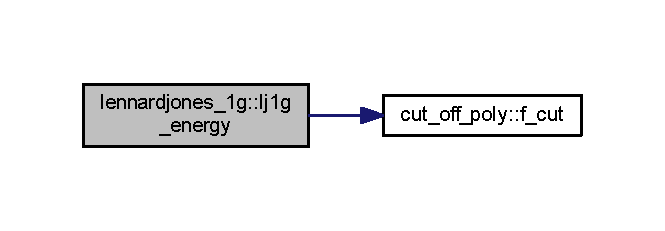
\includegraphics[width=319pt]{namespacelennardjones__1g_ad0b0c6184262c754f7daa91a179657ef_cgraph}
\end{center}
\end{figure}
\mbox{\Hypertarget{namespacelennardjones__1g_a2581bad1eb2a8f6b8ecaa6d09de8f226}\label{namespacelennardjones__1g_a2581bad1eb2a8f6b8ecaa6d09de8f226}} 
\index{lennardjones\+\_\+1g@{lennardjones\+\_\+1g}!lj1g\+\_\+forces@{lj1g\+\_\+forces}}
\index{lj1g\+\_\+forces@{lj1g\+\_\+forces}!lennardjones\+\_\+1g@{lennardjones\+\_\+1g}}
\subsubsection{\texorpdfstring{lj1g\+\_\+forces()}{lj1g\_forces()}}
{\footnotesize\ttfamily subroutine lennardjones\+\_\+1g\+::lj1g\+\_\+forces (\begin{DoxyParamCaption}\item[{type(\mbox{\hyperlink{structmd__general_1_1particles}{particles}})}]{atoms,  }\item[{type(\mbox{\hyperlink{structmd__general_1_1neighbour__list}{neighbour\+\_\+list}})}]{nl,  }\item[{type(\mbox{\hyperlink{structlennardjones__1g_1_1lennardjones1g__parameters}{lennardjones1g\+\_\+parameters}})}]{L\+Jp }\end{DoxyParamCaption})}



См. определение в файле Lennard\+Jones\+\_\+1g.\+f90 строка 52


\begin{DoxyCode}
52     \textcolor{keywordtype}{type}(particles) ::  atoms
53     \textcolor{keywordtype}{type}(neighbour\_list) :: nl
54     \textcolor{keywordtype}{type}(LennardJones1g\_parameters) :: LJp
55     \textcolor{keywordtype}{integer}:: i,p,k,ind,jnd
56     \textcolor{keywordtype}{real},\textcolor{keywordtype}{allocatable}:: priv\_force(:,:),F(:),fp(:,:)
57     
58     \textcolor{comment}{!$OMP PARALLEL private(i,p,k,ind,jnd,F,fp,priv\_force)}
59     \textcolor{keywordflow}{if}(.not. \textcolor{keyword}{allocated}(priv\_force)) \textcolor{keyword}{allocate}(priv\_force(3,atoms%N))\textcolor{comment}{!realloc if N changed}
60     \textcolor{keywordflow}{if}(.not. \textcolor{keyword}{allocated}(f)) \textcolor{keyword}{allocate}(f(nl%neighb\_num\_max))\textcolor{comment}{!realloc if neighb\_num\_max changed}
61     \textcolor{keywordflow}{if}(.not. \textcolor{keyword}{allocated}(fp)) \textcolor{keyword}{allocate}(fp(3,nl%neighb\_num\_max))\textcolor{comment}{!realloc if neighb\_num\_max changed}
62     f = 0.
63     fp = 0.
64     priv\_force = 0. 
65     \textcolor{comment}{!$OMP DO SCHEDULE(dynamic,chunk\_size)    }
66     \textcolor{keywordflow}{do} i=1,nl%N
67         \textcolor{keywordflow}{do} p=1,nl%lessnnum(i)
68             f(p) = scalar\_lj\_force(nl%moddr(p,i),ljp%R1,ljp%R2,ljp%c12,ljp%c6,ljp%c12t12,ljp%c6t6)
69 \textcolor{keywordflow}{        enddo}
70         \textcolor{keywordflow}{do} p=1,nl%lessnnum(i)
71             fp(1,p) = f(p)*nl%dr(1,p,i)
72             fp(2,p) = f(p)*nl%dr(2,p,i)
73             fp(3,p) = f(p)*nl%dr(3,p,i)
74 \textcolor{keywordflow}{        enddo}
75         \textcolor{keywordflow}{do} p=1,nl%lessnnum(i)
76             ind = nl%particle\_index(i)
77             jnd = nl%particle\_index(nl%nlist(p,i))
78             priv\_force(1,ind) = priv\_force(1,ind)-fp(1,p)
79             priv\_force(2,ind) = priv\_force(2,ind)-fp(2,p)
80             priv\_force(3,ind) = priv\_force(3,ind)-fp(3,p)
81             priv\_force(1,jnd) = priv\_force(1,jnd)+fp(1,p)
82             priv\_force(2,jnd) = priv\_force(2,jnd)+fp(2,p)
83             priv\_force(3,jnd) = priv\_force(3,jnd)+fp(3,p)
84 \textcolor{keywordflow}{        enddo}
85 \textcolor{keywordflow}{    enddo}
86     \textcolor{comment}{!$OMP END DO}
87     \textcolor{keywordflow}{do} i=1,nl%N
88         \textcolor{keywordflow}{do} k=1,3
89             \textcolor{comment}{!$OMP ATOMIC}
90                 atoms%forces(k,i) = atoms%forces(k,i)+priv\_force(k,i)
91 \textcolor{keywordflow}{        enddo}
92 \textcolor{keywordflow}{    enddo}
93     \textcolor{comment}{!$OMP END PARALLEL}
94     
\end{DoxyCode}
Граф вызовов\+:\nopagebreak
\begin{figure}[H]
\begin{center}
\leavevmode
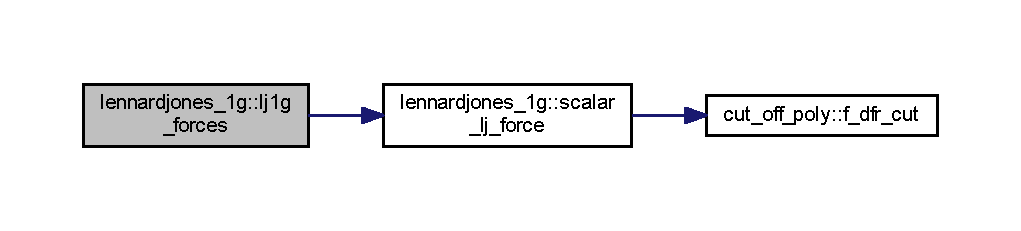
\includegraphics[width=350pt]{namespacelennardjones__1g_a2581bad1eb2a8f6b8ecaa6d09de8f226_cgraph}
\end{center}
\end{figure}
\mbox{\Hypertarget{namespacelennardjones__1g_aaf09aeeacdbe2a76adad336dde195938}\label{namespacelennardjones__1g_aaf09aeeacdbe2a76adad336dde195938}} 
\index{lennardjones\+\_\+1g@{lennardjones\+\_\+1g}!read\+\_\+lj1g\+\_\+parameters@{read\+\_\+lj1g\+\_\+parameters}}
\index{read\+\_\+lj1g\+\_\+parameters@{read\+\_\+lj1g\+\_\+parameters}!lennardjones\+\_\+1g@{lennardjones\+\_\+1g}}
\subsubsection{\texorpdfstring{read\+\_\+lj1g\+\_\+parameters()}{read\_lj1g\_parameters()}}
{\footnotesize\ttfamily subroutine lennardjones\+\_\+1g\+::read\+\_\+lj1g\+\_\+parameters (\begin{DoxyParamCaption}\item[{type(\mbox{\hyperlink{structlennardjones__1g_1_1lennardjones1g__parameters}{lennardjones1g\+\_\+parameters}})}]{L\+Jp,  }\item[{character($\ast$)}]{filename }\end{DoxyParamCaption})}



См. определение в файле Lennard\+Jones\+\_\+1g.\+f90 строка 14


\begin{DoxyCode}
14     \textcolor{keywordtype}{type}(LennardJones1g\_parameters):: LJp
15     \textcolor{keywordtype}{character(*)}::  filename
16     
17     \textcolor{keyword}{open}(1,file=filename)
18     \textcolor{keyword}{read}(1,*) ljp%eps,ljp%sig
19     \textcolor{keyword}{read}(1,*) ljp%R1,ljp%R2
20     \textcolor{keyword}{close}(1)
21     ljp%c6 = 4.*ljp%eps*ljp%sig**6
22     ljp%c12 = 4.*ljp%eps*ljp%sig**12
23     ljp%c6t6 = 6.*4.*ljp%eps*ljp%sig**6
24     ljp%c12t12 = 12.*4.*ljp%eps*ljp%sig**12
25     
\end{DoxyCode}
\mbox{\Hypertarget{namespacelennardjones__1g_a3bf6806cd81693117d84cb3f91adc6d5}\label{namespacelennardjones__1g_a3bf6806cd81693117d84cb3f91adc6d5}} 
\index{lennardjones\+\_\+1g@{lennardjones\+\_\+1g}!scalar\+\_\+lj\+\_\+force@{scalar\+\_\+lj\+\_\+force}}
\index{scalar\+\_\+lj\+\_\+force@{scalar\+\_\+lj\+\_\+force}!lennardjones\+\_\+1g@{lennardjones\+\_\+1g}}
\subsubsection{\texorpdfstring{scalar\+\_\+lj\+\_\+force()}{scalar\_lj\_force()}}
{\footnotesize\ttfamily real function lennardjones\+\_\+1g\+::scalar\+\_\+lj\+\_\+force (\begin{DoxyParamCaption}\item[{real, intent(in)}]{r,  }\item[{real, intent(in)}]{R1,  }\item[{real, intent(in)}]{R2,  }\item[{real, intent(in)}]{c12,  }\item[{real, intent(in)}]{c6,  }\item[{real, intent(in)}]{c12t12,  }\item[{real, intent(in)}]{c6t6 }\end{DoxyParamCaption})}



См. определение в файле Lennard\+Jones\+\_\+1g.\+f90 строка 98


\begin{DoxyCode}
98     \textcolor{comment}{!$OMP DECLARE SIMD(scalar\_lj\_force) UNIFORM(R1,R2,c12,c6,c12t12,c6t6)}
99     \textcolor{keywordtype}{real}, \textcolor{keywordtype}{intent(in)} :: r
100     \textcolor{keywordtype}{real}, \textcolor{keywordtype}{intent(in)} :: R1,R2,c12,c6,c12t12,c6t6
101     \textcolor{keywordtype}{real} scalar\_lj\_force
102     \textcolor{keywordtype}{real} :: invr2,U,fcut,dfrcut
103     
104     invr2 = 1./(r*r)
105     u = invr2*invr2*invr2
106     \textcolor{keyword}{call }f\_dfr\_cut(fcut,dfrcut,r,r1,r2)
107     scalar\_lj\_force = u*invr2*((c12t12*u-c6t6)*fcut-(c12*u-c6)*dfrcut)
108     
\end{DoxyCode}
Граф вызовов\+:\nopagebreak
\begin{figure}[H]
\begin{center}
\leavevmode
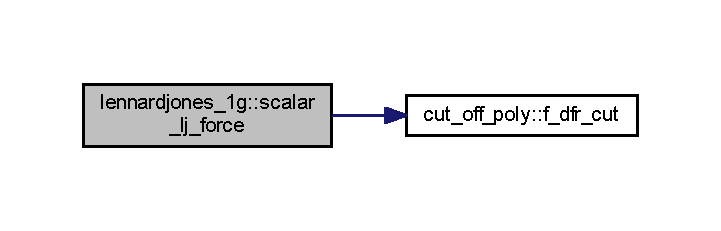
\includegraphics[width=346pt]{namespacelennardjones__1g_a3bf6806cd81693117d84cb3f91adc6d5_cgraph}
\end{center}
\end{figure}

\hypertarget{namespacelennardjonescosine}{}\section{Модуль lennardjonescosine}
\label{namespacelennardjonescosine}\index{lennardjonescosine@{lennardjonescosine}}
\subsection*{Типы данных}
\begin{DoxyCompactItemize}
\item 
type \mbox{\hyperlink{structlennardjonescosine_1_1lennardjonescosine__parameters}{lennardjonescosine\+\_\+parameters}}
\end{DoxyCompactItemize}
\subsection*{Функции/подпрограммы}
\begin{DoxyCompactItemize}
\item 
subroutine \mbox{\hyperlink{namespacelennardjonescosine_abdcce4a33286a32fa7d04e2fd1344934}{read\+\_\+ljc\+\_\+parameters}} (L\+J\+Cp, filename)
\item 
subroutine \mbox{\hyperlink{namespacelennardjonescosine_a50bfc170eedcf42dd2252426f2476002}{ljc\+\_\+energy}} (energy, nl, L\+J\+Cp)
\item 
subroutine \mbox{\hyperlink{namespacelennardjonescosine_aa355c58f69eacc410be4c84a216f9aeb}{ljc\+\_\+forces\+\_\+for\+\_\+graphene}} (atoms, nl, nl\+\_\+nn, L\+J\+Cp)
\item 
subroutine \mbox{\hyperlink{namespacelennardjonescosine_a73608f731b0cb701778f6b125e057ab4}{ljc\+\_\+forces\+\_\+for\+\_\+other\+\_\+atoms}} (atoms, nl, L\+J\+Cp)
\end{DoxyCompactItemize}


\subsection{Функции/подпрограммы}
\mbox{\Hypertarget{namespacelennardjonescosine_a50bfc170eedcf42dd2252426f2476002}\label{namespacelennardjonescosine_a50bfc170eedcf42dd2252426f2476002}} 
\index{lennardjonescosine@{lennardjonescosine}!ljc\+\_\+energy@{ljc\+\_\+energy}}
\index{ljc\+\_\+energy@{ljc\+\_\+energy}!lennardjonescosine@{lennardjonescosine}}
\subsubsection{\texorpdfstring{ljc\+\_\+energy()}{ljc\_energy()}}
{\footnotesize\ttfamily subroutine lennardjonescosine\+::ljc\+\_\+energy (\begin{DoxyParamCaption}\item[{real}]{energy,  }\item[{type(\mbox{\hyperlink{structmd__general_1_1neighbour__list}{neighbour\+\_\+list}})}]{nl,  }\item[{type(\mbox{\hyperlink{structlennardjonescosine_1_1lennardjonescosine__parameters}{lennardjonescosine\+\_\+parameters}})}]{L\+J\+Cp }\end{DoxyParamCaption})}



См. определение в файле Lennard\+Jones\+Cosine.\+f90 строка 27


\begin{DoxyCode}
27     \textcolor{keywordtype}{type}(neighbour\_list):: nl
28     \textcolor{keywordtype}{type}(LennardJonesCosine\_parameters):: LJCp
29     \textcolor{keywordtype}{integer}:: i,p
30     \textcolor{keywordtype}{real}:: energy,energy\_priv,V1,V2,V3
31     
32     energy = 0.
33     energy\_priv = 0.
34     \textcolor{comment}{!$OMP PARALLEL firstprivate(energy\_priv,i,p,V1,V2,V3)}
35     \textcolor{comment}{!$OMP DO}
36     \textcolor{keywordflow}{do} i=1,nl%N
37         \textcolor{keywordflow}{do} p=1,nl%nnum(i)
38             \textcolor{keywordflow}{if} (nl%moddr(p,i)<ljcp%R2) \textcolor{keywordflow}{then}
39                 v2 = (ljcp%sig/nl%moddr(p,i))**6
40                 v1 = v2**2
41                 v3 = (abs(sum(ljcp%gr\_norm(:,i)*nl%dr(:,p,i)))/nl%moddr(p,i))**ljcp%delt
42                 energy\_priv = energy\_priv+4*ljcp%eps*(v1-v2*v3)*f\_cut(nl%moddr(p,i),ljcp%R1,ljcp%R2)
43 \textcolor{keywordflow}{            endif}   
44 \textcolor{keywordflow}{        enddo}
45 \textcolor{keywordflow}{    enddo}
46     \textcolor{comment}{!$OMP END DO}
47     \textcolor{comment}{!$OMP ATOMIC}
48         energy = energy+energy\_priv
49     \textcolor{comment}{!$OMP END PARALLEL}
50     
\end{DoxyCode}
Граф вызовов\+:\nopagebreak
\begin{figure}[H]
\begin{center}
\leavevmode
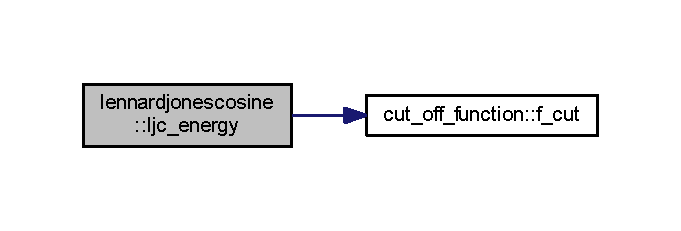
\includegraphics[width=327pt]{namespacelennardjonescosine_a50bfc170eedcf42dd2252426f2476002_cgraph}
\end{center}
\end{figure}
\mbox{\Hypertarget{namespacelennardjonescosine_aa355c58f69eacc410be4c84a216f9aeb}\label{namespacelennardjonescosine_aa355c58f69eacc410be4c84a216f9aeb}} 
\index{lennardjonescosine@{lennardjonescosine}!ljc\+\_\+forces\+\_\+for\+\_\+graphene@{ljc\+\_\+forces\+\_\+for\+\_\+graphene}}
\index{ljc\+\_\+forces\+\_\+for\+\_\+graphene@{ljc\+\_\+forces\+\_\+for\+\_\+graphene}!lennardjonescosine@{lennardjonescosine}}
\subsubsection{\texorpdfstring{ljc\+\_\+forces\+\_\+for\+\_\+graphene()}{ljc\_forces\_for\_graphene()}}
{\footnotesize\ttfamily subroutine lennardjonescosine\+::ljc\+\_\+forces\+\_\+for\+\_\+graphene (\begin{DoxyParamCaption}\item[{type(\mbox{\hyperlink{structmd__general_1_1particles}{particles}})}]{atoms,  }\item[{type(\mbox{\hyperlink{structmd__general_1_1neighbour__list}{neighbour\+\_\+list}})}]{nl,  }\item[{type(\mbox{\hyperlink{structmd__general_1_1neighbour__list}{neighbour\+\_\+list}})}]{nl\+\_\+nn,  }\item[{type(\mbox{\hyperlink{structlennardjonescosine_1_1lennardjonescosine__parameters}{lennardjonescosine\+\_\+parameters}})}]{L\+J\+Cp }\end{DoxyParamCaption})}



См. определение в файле Lennard\+Jones\+Cosine.\+f90 строка 54


\begin{DoxyCode}
54     \textcolor{keywordtype}{type}(particles)::   atoms
55     \textcolor{keywordtype}{type}(neighbour\_list):: nl,nl\_nn
56     \textcolor{keywordtype}{type}(LennardJonesCosine\_parameters):: LJCp
57     \textcolor{keywordtype}{integer}:: i,p,q,l1,l2,l3,j,k,nnum\_nn
58     \textcolor{keywordtype}{real}:: drj12(3),drj31(3),drj23(3),V1,V2,V3,f\_c,df\_c
59     
60     \textcolor{keywordflow}{if} (nl%N/=nl\_nn%N .and. nl%N/=0) then; \textcolor{keyword}{write}(*,*) \textcolor{stringliteral}{'error: nl%N/=nl\_nn%N'},nl%N,nl\_nn%N; stop;\textcolor{keywordflow}{ endif}
61     nnum\_nn = 3
62     \textcolor{keywordflow}{if} (ljcp%simplified) then; nnum\_nn = 0; ljcp%gr\_norm = 0.; ljcp%gr\_norm(3,:) = 1.; endif\textcolor{comment}{!optimize}
63     
64     \textcolor{comment}{!$OMP PARALLEL firstprivate(i,p,q,l1,l2,l3,j,k,drj12,drj31,drj23,V1,V2,V3,f\_c,df\_c)}
65     \textcolor{comment}{!$OMP DO}
66     \textcolor{keywordflow}{do} i=1,nl%N
67         \textcolor{keywordflow}{do} p=1,nl%nnum(i)
68             \textcolor{keywordflow}{if} (nl%moddr(p,i)<ljcp%R2) \textcolor{keywordflow}{then}
69                 v2 = (ljcp%sig/nl%moddr(p,i))**6
70                 v1 = v2**2
71                 v3 = (abs(sum(ljcp%gr\_norm(:,i)*nl%dr(:,p,i)))/nl%moddr(p,i))**ljcp%delt
72                 f\_c = f\_cut(nl%moddr(p,i),ljcp%R1,ljcp%R2)
73                 df\_c = df\_cut(nl%moddr(p,i),ljcp%R1,ljcp%R2)
74                 atoms%forces(:,nl%particle\_index(i)) = atoms%forces(:,nl%particle\_index(i))-4.*ljcp%eps*&
75                 (((12.*v1-(6.+ljcp%delt)*v2*v3)/nl%moddr(p,i)**2*f\_c-(v1-v2*v3)*df\_c)*nl%dr(:,p,i)+&
76                 (ljcp%delt*v2*v3/sum(ljcp%gr\_norm(:,i)*nl%dr(:,p,i))*f\_c)*ljcp%gr\_norm(:,i))
77 \textcolor{keywordflow}{            endif}
78 \textcolor{keywordflow}{        enddo}
79 \textcolor{keywordflow}{    enddo}
80     \textcolor{comment}{!$OMP END DO}
81     \textcolor{comment}{!$OMP DO}
82     \textcolor{keywordflow}{do} i=1,nl%N
83         \textcolor{keywordflow}{do} q=1,nnum\_nn
84             j = nl\_nn%nlist(q,i)
85             \textcolor{keywordflow}{do} l1=1,nnum\_nn
86                 \textcolor{keywordflow}{if} (nl\_nn%nlist(l1,j)==i) \textcolor{keywordflow}{exit}
87 \textcolor{keywordflow}{            enddo}
88             \textcolor{keywordflow}{if}(l1>3) then; \textcolor{keyword}{write}(*,*) \textcolor{stringliteral}{'l1>3'}; stop;\textcolor{keywordflow}{ endif}
89             l2 = mod(l1,3)+1
90             l3 = mod(l1+1,3)+1
91             drj12 = nl\_nn%dr(:,l2,j)-nl\_nn%dr(:,l1,j)
92             drj31 = nl\_nn%dr(:,l1,j)-nl\_nn%dr(:,l3,j)
93             drj23 = nl\_nn%dr(:,l3,j)-nl\_nn%dr(:,l2,j)
94             \textcolor{keywordflow}{do} p=1,nl%nnum(j)
95                 \textcolor{keywordflow}{if} (nl%moddr(p,j)<ljcp%R2) \textcolor{keywordflow}{then}
96                     v2 = (ljcp%sig/nl%moddr(p,j))**6
97                     v1 = v2**2
98                     v3 = (abs(sum(ljcp%gr\_norm(:,j)*nl%dr(:,p,j)))/nl%moddr(p,j))**ljcp%delt
99                     f\_c = f\_cut(nl%moddr(p,j),ljcp%R1,ljcp%R2)
100                     atoms%forces(:,nl%particle\_index(i)) = atoms%forces(:,nl%particle\_index(i))&
101                     -4.*ljcp%eps*ljcp%delt*v2*v3*f\_c/(sum(drj12**2)*sum(drj31**2)-sum(drj12*drj31)**2)/sum(
      ljcp%gr\_norm(:,j)*nl%dr(:,p,j))*&
102                     ljcp%gr\_norm(:,j)*sum(nl%dr(:,p,j)*(drj12*sum(drj23*drj31)-drj31*sum(drj23*drj12)))
103 \textcolor{keywordflow}{                endif}
104 \textcolor{keywordflow}{            enddo}
105 \textcolor{keywordflow}{        enddo}
106 \textcolor{keywordflow}{    enddo}
107     \textcolor{comment}{!$OMP END DO}
108     \textcolor{comment}{!$OMP END PARALLEL}
109     
\end{DoxyCode}
Граф вызовов\+:\nopagebreak
\begin{figure}[H]
\begin{center}
\leavevmode
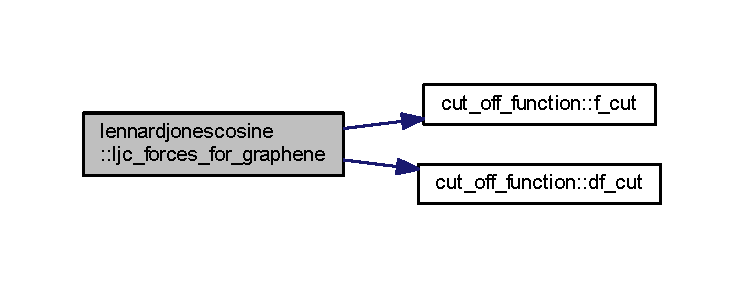
\includegraphics[width=350pt]{namespacelennardjonescosine_aa355c58f69eacc410be4c84a216f9aeb_cgraph}
\end{center}
\end{figure}
\mbox{\Hypertarget{namespacelennardjonescosine_a73608f731b0cb701778f6b125e057ab4}\label{namespacelennardjonescosine_a73608f731b0cb701778f6b125e057ab4}} 
\index{lennardjonescosine@{lennardjonescosine}!ljc\+\_\+forces\+\_\+for\+\_\+other\+\_\+atoms@{ljc\+\_\+forces\+\_\+for\+\_\+other\+\_\+atoms}}
\index{ljc\+\_\+forces\+\_\+for\+\_\+other\+\_\+atoms@{ljc\+\_\+forces\+\_\+for\+\_\+other\+\_\+atoms}!lennardjonescosine@{lennardjonescosine}}
\subsubsection{\texorpdfstring{ljc\+\_\+forces\+\_\+for\+\_\+other\+\_\+atoms()}{ljc\_forces\_for\_other\_atoms()}}
{\footnotesize\ttfamily subroutine lennardjonescosine\+::ljc\+\_\+forces\+\_\+for\+\_\+other\+\_\+atoms (\begin{DoxyParamCaption}\item[{type(\mbox{\hyperlink{structmd__general_1_1particles}{particles}})}]{atoms,  }\item[{type(\mbox{\hyperlink{structmd__general_1_1neighbour__list}{neighbour\+\_\+list}})}]{nl,  }\item[{type(\mbox{\hyperlink{structlennardjonescosine_1_1lennardjonescosine__parameters}{lennardjonescosine\+\_\+parameters}})}]{L\+J\+Cp }\end{DoxyParamCaption})}



См. определение в файле Lennard\+Jones\+Cosine.\+f90 строка 113


\begin{DoxyCode}
113     \textcolor{keywordtype}{type}(particles)::   atoms
114     \textcolor{keywordtype}{type}(neighbour\_list):: nl
115     \textcolor{keywordtype}{type}(LennardJonesCosine\_parameters):: LJCp
116     \textcolor{keywordtype}{integer}:: i,p
117     \textcolor{keywordtype}{real}:: gr\_n(3),V1,V2,V3,f\_c,df\_c
118     
119     \textcolor{comment}{!$OMP PARALLEL firstprivate(i,p,gr\_n,V1,V2,V3,f\_c,df\_c)}
120     \textcolor{comment}{!$OMP DO}
121     \textcolor{keywordflow}{do} i=1,nl%N
122         \textcolor{keywordflow}{do} p=1,nl%nnum(i)
123             \textcolor{keywordflow}{if} (nl%moddr(p,i)<ljcp%R2) \textcolor{keywordflow}{then}
124                 gr\_n = ljcp%gr\_norm(:,nl%nlist(p,i))
125                 v2 = (ljcp%sig/nl%moddr(p,i))**6
126                 v1 = v2**2
127                 v3 = (abs(sum(gr\_n*nl%dr(:,p,i)))/nl%moddr(p,i))**ljcp%delt
128                 f\_c = f\_cut(nl%moddr(p,i),ljcp%R1,ljcp%R2)
129                 df\_c = df\_cut(nl%moddr(p,i),ljcp%R1,ljcp%R2)
130                 atoms%forces(:,nl%particle\_index(i)) = atoms%forces(:,nl%particle\_index(i))-4.*ljcp%eps*&
131                 (((12.*v1-(6.+ljcp%delt)*v2*v3)/nl%moddr(p,i)**2*f\_c-(v1-v2*v3)*df\_c)*nl%dr(:,p,i)+&
132                 (ljcp%delt*v2*v3/sum(gr\_n*nl%dr(:,p,i))*f\_c)*gr\_n)
133 \textcolor{keywordflow}{            endif}
134 \textcolor{keywordflow}{        enddo}
135 \textcolor{keywordflow}{    enddo}
136     \textcolor{comment}{!$OMP END DO }
137     \textcolor{comment}{!$OMP END PARALLEL}
138     
\end{DoxyCode}
Граф вызовов\+:\nopagebreak
\begin{figure}[H]
\begin{center}
\leavevmode
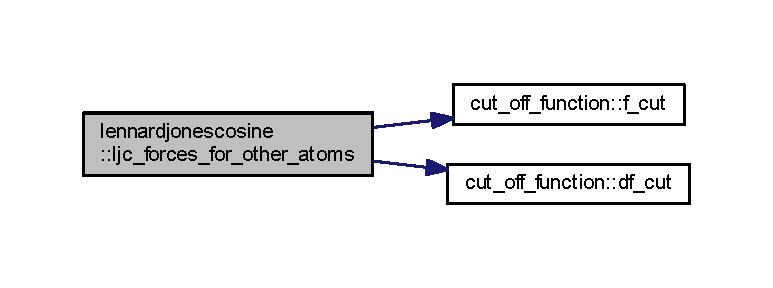
\includegraphics[width=350pt]{namespacelennardjonescosine_a73608f731b0cb701778f6b125e057ab4_cgraph}
\end{center}
\end{figure}
\mbox{\Hypertarget{namespacelennardjonescosine_abdcce4a33286a32fa7d04e2fd1344934}\label{namespacelennardjonescosine_abdcce4a33286a32fa7d04e2fd1344934}} 
\index{lennardjonescosine@{lennardjonescosine}!read\+\_\+ljc\+\_\+parameters@{read\+\_\+ljc\+\_\+parameters}}
\index{read\+\_\+ljc\+\_\+parameters@{read\+\_\+ljc\+\_\+parameters}!lennardjonescosine@{lennardjonescosine}}
\subsubsection{\texorpdfstring{read\+\_\+ljc\+\_\+parameters()}{read\_ljc\_parameters()}}
{\footnotesize\ttfamily subroutine lennardjonescosine\+::read\+\_\+ljc\+\_\+parameters (\begin{DoxyParamCaption}\item[{type(\mbox{\hyperlink{structlennardjonescosine_1_1lennardjonescosine__parameters}{lennardjonescosine\+\_\+parameters}})}]{L\+J\+Cp,  }\item[{character($\ast$)}]{filename }\end{DoxyParamCaption})}



См. определение в файле Lennard\+Jones\+Cosine.\+f90 строка 15


\begin{DoxyCode}
15     \textcolor{keywordtype}{type}(LennardJonesCosine\_parameters):: LJCp
16     \textcolor{keywordtype}{character(*)}::  filename
17     
18     \textcolor{keyword}{open}(1,file=filename)
19     \textcolor{keyword}{read}(1,*) ljcp%eps,ljcp%sig,ljcp%delt
20     \textcolor{keyword}{read}(1,*) ljcp%R1,ljcp%R2
21     \textcolor{keyword}{read}(1,*) ljcp%simplified
22     \textcolor{keyword}{close}(1)
23     
\end{DoxyCode}

\hypertarget{namespacemd__general}{}\section{Модуль md\+\_\+general}
\label{namespacemd__general}\index{md\+\_\+general@{md\+\_\+general}}
\subsection*{Типы данных}
\begin{DoxyCompactItemize}
\item 
type \mbox{\hyperlink{structmd__general_1_1integrator__params}{integrator\+\_\+params}}
\item 
type \mbox{\hyperlink{structmd__general_1_1neighbour__list}{neighbour\+\_\+list}}
\item 
type \mbox{\hyperlink{structmd__general_1_1nose__hoover__chain}{nose\+\_\+hoover\+\_\+chain}}
\item 
type \mbox{\hyperlink{structmd__general_1_1particle__group}{particle\+\_\+group}}
\item 
type \mbox{\hyperlink{structmd__general_1_1particles}{particles}}
\item 
type \mbox{\hyperlink{structmd__general_1_1simulation__cell}{simulation\+\_\+cell}}
\item 
type \mbox{\hyperlink{structmd__general_1_1time__steps}{time\+\_\+steps}}
\end{DoxyCompactItemize}
\subsection*{Функции/подпрограммы}
\begin{DoxyCompactItemize}
\item 
subroutine \mbox{\hyperlink{namespacemd__general_a3a69c40fe5a6e7938d398f803b21e474}{init\+\_\+time\+\_\+steps}} (dt, delta\+\_\+t)
\item 
subroutine \mbox{\hyperlink{namespacemd__general_a6e847bdd3b7115bf5ff69e8cd8e68d7f}{create\+\_\+particle\+\_\+group}} (group, type\+\_\+names, atoms)
\item 
subroutine \mbox{\hyperlink{namespacemd__general_a5614c27d83ed003aa01d3be2f1b45c57}{change\+\_\+particle\+\_\+group\+\_\+n}} (group, md\+\_\+step, change\+\_\+ts1, change\+\_\+ts2, change\+\_\+frec, init\+\_\+group)
\item 
subroutine \mbox{\hyperlink{namespacemd__general_ad4ad26fa9584c63f846d49033ce92987}{scale\+\_\+velocities}} (atoms, group, s)
\item 
subroutine \mbox{\hyperlink{namespacemd__general_a326a2fe1c1da84197c4566801133648a}{random\+\_\+velocities}} (atoms, group)
\item 
subroutine \mbox{\hyperlink{namespacemd__general_a8192b37ec3462b5fcb7fabf17c8eb658}{random\+\_\+momenta}} (atoms, group)
\item 
subroutine \mbox{\hyperlink{namespacemd__general_a0949b9217f73c42e2c7ea47a4e559e39}{calculate\+\_\+kinetic\+\_\+energy}} (ke, atoms, group)
\item 
subroutine \mbox{\hyperlink{namespacemd__general_aafe7eb801a25cbfeff68d5574b9fc152}{calculate\+\_\+mass\+\_\+center}} (mc, atoms, group)
\item 
subroutine \mbox{\hyperlink{namespacemd__general_a39191e16e77e39d5486e4daaeaa2522e}{calculate\+\_\+mass\+\_\+center\+\_\+velosity}} (mcv, atoms, group)
\item 
subroutine \mbox{\hyperlink{namespacemd__general_a79ea9e512a27c651278559e30f97a336}{zero\+\_\+momentum}} (atoms, group)
\item 
subroutine \mbox{\hyperlink{namespacemd__general_a77b50b971bc4812a1299348a398491e0}{calculate\+\_\+masses\+\_\+sum}} (totm, atoms, group)
\item 
subroutine \mbox{\hyperlink{namespacemd__general_ac5733857b75ce71aa32a105751e4dfd5}{calculate\+\_\+force\+\_\+sum}} (fs, atoms, group)
\item 
subroutine \mbox{\hyperlink{namespacemd__general_a1de2d09f44a8dc5b96fc5eb221845cc1}{calculate\+\_\+temperature}} (temp, ke, atoms, group)
\item 
subroutine \mbox{\hyperlink{namespacemd__general_a9f99fa4920c9047597f37b777dd44b3c}{set\+\_\+new\+\_\+temperature}} (atoms, group, temp)
\item 
subroutine \mbox{\hyperlink{namespacemd__general_ac9e62480edf60d2b3d1a123c9da68e1f}{check\+\_\+positions}} (out\+\_\+id, atoms, box)
\item 
subroutine \mbox{\hyperlink{namespacemd__general_abd425450c2140a07748c79f0f0dbd760}{check\+\_\+velocities}} (out\+\_\+id, atoms)
\item 
subroutine \mbox{\hyperlink{namespacemd__general_aca48dc12ea3fb99991acd82c2223a9bf}{invert\+\_\+z\+\_\+velocities}} (atoms, z\+\_\+low\+\_\+border, z\+\_\+high\+\_\+border)
\item 
subroutine \mbox{\hyperlink{namespacemd__general_a5dc45690a2125a86ce58d01601ebdf45}{position\+\_\+analysis}} (av, mi, ma, atoms, group, direction, minimum, maximum)
\item 
pure subroutine \mbox{\hyperlink{namespacemd__general_a33570f37733690b0634f039ad1bcf35e}{find\+\_\+distance}} (dr, dr2, vec1, vec2, box)
\end{DoxyCompactItemize}


\subsection{Функции/подпрограммы}
\mbox{\Hypertarget{namespacemd__general_ac5733857b75ce71aa32a105751e4dfd5}\label{namespacemd__general_ac5733857b75ce71aa32a105751e4dfd5}} 
\index{md\+\_\+general@{md\+\_\+general}!calculate\+\_\+force\+\_\+sum@{calculate\+\_\+force\+\_\+sum}}
\index{calculate\+\_\+force\+\_\+sum@{calculate\+\_\+force\+\_\+sum}!md\+\_\+general@{md\+\_\+general}}
\subsubsection{\texorpdfstring{calculate\+\_\+force\+\_\+sum()}{calculate\_force\_sum()}}
{\footnotesize\ttfamily subroutine md\+\_\+general\+::calculate\+\_\+force\+\_\+sum (\begin{DoxyParamCaption}\item[{real, dimension(3)}]{fs,  }\item[{type(\mbox{\hyperlink{structmd__general_1_1particles}{particles}})}]{atoms,  }\item[{type(\mbox{\hyperlink{structmd__general_1_1particle__group}{particle\+\_\+group}})}]{group }\end{DoxyParamCaption})}



См. определение в файле md\+\_\+general.\+f90 строка 279


\begin{DoxyCode}
279     \textcolor{keywordtype}{type}(particles)::   atoms
280     \textcolor{keywordtype}{type}(particle\_group):: group
281     \textcolor{keywordtype}{real}:: fs(3),fs\_priv(3)
282     \textcolor{keywordtype}{integer}::       i,ind,k
283 
284     fs = 0.
285     fs\_priv = 0.
286     \textcolor{comment}{!$OMP PARALLEL firstprivate(fs\_priv,i,ind,k)}
287     \textcolor{comment}{!$OMP DO}
288     \textcolor{keywordflow}{do} ind=1,group%N
289         i = group%indexes(ind)
290         fs\_priv = fs\_priv+atoms%forces(:,i)
291 \textcolor{keywordflow}{    enddo}
292     \textcolor{comment}{!$OMP END DO}
293     \textcolor{keywordflow}{do} k=1,3
294         \textcolor{comment}{!$OMP ATOMIC}
295             fs(k) = fs(k)+fs\_priv(k)
296 \textcolor{keywordflow}{    enddo}
297     \textcolor{comment}{!$OMP END PARALLEL}
298 
299     \textcolor{keywordflow}{return}
\end{DoxyCode}
\mbox{\Hypertarget{namespacemd__general_a0949b9217f73c42e2c7ea47a4e559e39}\label{namespacemd__general_a0949b9217f73c42e2c7ea47a4e559e39}} 
\index{md\+\_\+general@{md\+\_\+general}!calculate\+\_\+kinetic\+\_\+energy@{calculate\+\_\+kinetic\+\_\+energy}}
\index{calculate\+\_\+kinetic\+\_\+energy@{calculate\+\_\+kinetic\+\_\+energy}!md\+\_\+general@{md\+\_\+general}}
\subsubsection{\texorpdfstring{calculate\+\_\+kinetic\+\_\+energy()}{calculate\_kinetic\_energy()}}
{\footnotesize\ttfamily subroutine md\+\_\+general\+::calculate\+\_\+kinetic\+\_\+energy (\begin{DoxyParamCaption}\item[{real}]{ke,  }\item[{type(\mbox{\hyperlink{structmd__general_1_1particles}{particles}})}]{atoms,  }\item[{type(\mbox{\hyperlink{structmd__general_1_1particle__group}{particle\+\_\+group}})}]{group }\end{DoxyParamCaption})}



См. определение в файле md\+\_\+general.\+f90 строка 163


\begin{DoxyCode}
163     \textcolor{keywordtype}{type}(particles)::   atoms
164     \textcolor{keywordtype}{type}(particle\_group):: group
165     \textcolor{keywordtype}{real}:: ke,ke\_priv
166     \textcolor{keywordtype}{real},\textcolor{keywordtype}{parameter}:: mass\_coef=1.6605389217/1.6021765654*10.**(2)
167     \textcolor{keywordtype}{integer}::       i,ind
168 
169     ke = 0.
170     ke\_priv = 0.
171     \textcolor{comment}{!$OMP PARALLEL firstprivate(ke\_priv,i,ind)}
172     \textcolor{comment}{!$OMP DO}
173     \textcolor{keywordflow}{do} ind=1,group%N
174         i = group%indexes(ind)
175         ke\_priv = ke\_priv+atoms%masses(i)*sum(atoms%velocities(:,i)**2)/2*mass\_coef
176 \textcolor{keywordflow}{    enddo}
177     \textcolor{comment}{!$OMP END DO}
178     \textcolor{comment}{!$OMP ATOMIC}
179         ke = ke+ke\_priv
180     \textcolor{comment}{!$OMP END PARALLEL}
181 
182     \textcolor{keywordflow}{return}
\end{DoxyCode}
\mbox{\Hypertarget{namespacemd__general_aafe7eb801a25cbfeff68d5574b9fc152}\label{namespacemd__general_aafe7eb801a25cbfeff68d5574b9fc152}} 
\index{md\+\_\+general@{md\+\_\+general}!calculate\+\_\+mass\+\_\+center@{calculate\+\_\+mass\+\_\+center}}
\index{calculate\+\_\+mass\+\_\+center@{calculate\+\_\+mass\+\_\+center}!md\+\_\+general@{md\+\_\+general}}
\subsubsection{\texorpdfstring{calculate\+\_\+mass\+\_\+center()}{calculate\_mass\_center()}}
{\footnotesize\ttfamily subroutine md\+\_\+general\+::calculate\+\_\+mass\+\_\+center (\begin{DoxyParamCaption}\item[{real, dimension(3)}]{mc,  }\item[{type(\mbox{\hyperlink{structmd__general_1_1particles}{particles}})}]{atoms,  }\item[{type(\mbox{\hyperlink{structmd__general_1_1particle__group}{particle\+\_\+group}})}]{group }\end{DoxyParamCaption})}



См. определение в файле md\+\_\+general.\+f90 строка 186


\begin{DoxyCode}
186     \textcolor{keywordtype}{type}(particles)::   atoms
187     \textcolor{keywordtype}{type}(particle\_group):: group
188     \textcolor{keywordtype}{real}:: mc(3),mc\_priv(3),totm
189     \textcolor{keywordtype}{integer}::       i,ind,k
190 
191     mc = 0.
192     mc\_priv = 0.
193     \textcolor{comment}{!$OMP PARALLEL firstprivate(mc\_priv,i,ind,k)}
194     \textcolor{comment}{!$OMP DO}
195     \textcolor{keywordflow}{do} ind=1,group%N
196         i = group%indexes(ind)
197         mc\_priv = mc\_priv+atoms%masses(i)*atoms%positions(:,i)
198 \textcolor{keywordflow}{    enddo}
199     \textcolor{comment}{!$OMP END DO}
200     \textcolor{keywordflow}{do} k=1,3
201         \textcolor{comment}{!$OMP ATOMIC}
202             mc(k) = mc(k)+mc\_priv(k)
203 \textcolor{keywordflow}{    enddo}
204     \textcolor{comment}{!$OMP END PARALLEL}
205     \textcolor{keyword}{call }calculate\_masses\_sum(totm,atoms,group)
206     mc = mc/totm
207 
208     \textcolor{keywordflow}{return}
\end{DoxyCode}
Граф вызовов\+:\nopagebreak
\begin{figure}[H]
\begin{center}
\leavevmode
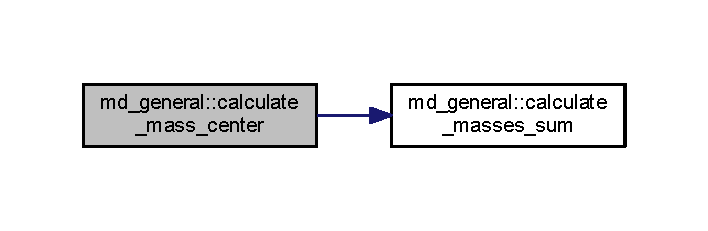
\includegraphics[width=340pt]{namespacemd__general_aafe7eb801a25cbfeff68d5574b9fc152_cgraph}
\end{center}
\end{figure}
\mbox{\Hypertarget{namespacemd__general_a39191e16e77e39d5486e4daaeaa2522e}\label{namespacemd__general_a39191e16e77e39d5486e4daaeaa2522e}} 
\index{md\+\_\+general@{md\+\_\+general}!calculate\+\_\+mass\+\_\+center\+\_\+velosity@{calculate\+\_\+mass\+\_\+center\+\_\+velosity}}
\index{calculate\+\_\+mass\+\_\+center\+\_\+velosity@{calculate\+\_\+mass\+\_\+center\+\_\+velosity}!md\+\_\+general@{md\+\_\+general}}
\subsubsection{\texorpdfstring{calculate\+\_\+mass\+\_\+center\+\_\+velosity()}{calculate\_mass\_center\_velosity()}}
{\footnotesize\ttfamily subroutine md\+\_\+general\+::calculate\+\_\+mass\+\_\+center\+\_\+velosity (\begin{DoxyParamCaption}\item[{real, dimension(3)}]{mcv,  }\item[{type(\mbox{\hyperlink{structmd__general_1_1particles}{particles}})}]{atoms,  }\item[{type(\mbox{\hyperlink{structmd__general_1_1particle__group}{particle\+\_\+group}})}]{group }\end{DoxyParamCaption})}



См. определение в файле md\+\_\+general.\+f90 строка 212


\begin{DoxyCode}
212     \textcolor{keywordtype}{type}(particles)::   atoms
213     \textcolor{keywordtype}{type}(particle\_group):: group
214     \textcolor{keywordtype}{real}:: mcv(3),mcv\_priv(3),totm
215     \textcolor{keywordtype}{integer}::       i,ind,k
216 
217     mcv = 0.
218     mcv\_priv = 0.
219     \textcolor{comment}{!$OMP PARALLEL firstprivate(mcv\_priv,i,ind,k)}
220     \textcolor{comment}{!$OMP DO}
221     \textcolor{keywordflow}{do} ind=1,group%N
222         i = group%indexes(ind)
223         mcv\_priv = mcv\_priv+atoms%masses(i)*atoms%velocities(:,i)
224 \textcolor{keywordflow}{    enddo}
225     \textcolor{comment}{!$OMP END DO}
226     \textcolor{keywordflow}{do} k=1,3
227         \textcolor{comment}{!$OMP ATOMIC}
228             mcv(k) = mcv(k)+mcv\_priv(k)
229 \textcolor{keywordflow}{    enddo}
230     \textcolor{comment}{!$OMP END PARALLEL}
231     \textcolor{keyword}{call }calculate\_masses\_sum(totm,atoms,group)
232     mcv = mcv/totm
233 
234     \textcolor{keywordflow}{return}
\end{DoxyCode}
Граф вызовов\+:\nopagebreak
\begin{figure}[H]
\begin{center}
\leavevmode
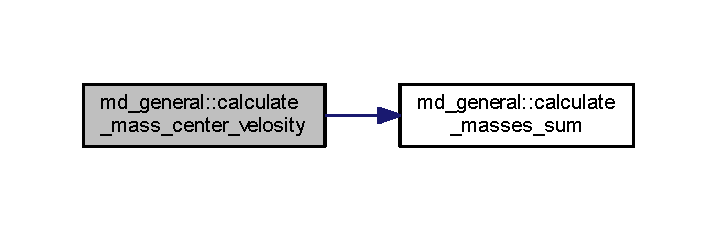
\includegraphics[width=344pt]{namespacemd__general_a39191e16e77e39d5486e4daaeaa2522e_cgraph}
\end{center}
\end{figure}
\mbox{\Hypertarget{namespacemd__general_a77b50b971bc4812a1299348a398491e0}\label{namespacemd__general_a77b50b971bc4812a1299348a398491e0}} 
\index{md\+\_\+general@{md\+\_\+general}!calculate\+\_\+masses\+\_\+sum@{calculate\+\_\+masses\+\_\+sum}}
\index{calculate\+\_\+masses\+\_\+sum@{calculate\+\_\+masses\+\_\+sum}!md\+\_\+general@{md\+\_\+general}}
\subsubsection{\texorpdfstring{calculate\+\_\+masses\+\_\+sum()}{calculate\_masses\_sum()}}
{\footnotesize\ttfamily subroutine md\+\_\+general\+::calculate\+\_\+masses\+\_\+sum (\begin{DoxyParamCaption}\item[{real}]{totm,  }\item[{type(\mbox{\hyperlink{structmd__general_1_1particles}{particles}})}]{atoms,  }\item[{type(\mbox{\hyperlink{structmd__general_1_1particle__group}{particle\+\_\+group}})}]{group }\end{DoxyParamCaption})}



См. определение в файле md\+\_\+general.\+f90 строка 257


\begin{DoxyCode}
257     \textcolor{keywordtype}{type}(particles)::   atoms
258     \textcolor{keywordtype}{type}(particle\_group):: group
259     \textcolor{keywordtype}{real}:: totm,totm\_priv
260     \textcolor{keywordtype}{integer}::       i,ind
261 
262     totm = 0.
263     totm\_priv = 0.
264     \textcolor{comment}{!$OMP PARALLEL firstprivate(totm\_priv,i,ind)}
265     \textcolor{comment}{!$OMP DO}
266     \textcolor{keywordflow}{do} ind=1,group%N
267         i = group%indexes(ind)
268         totm\_priv = totm\_priv+atoms%masses(i)
269 \textcolor{keywordflow}{    enddo}
270     \textcolor{comment}{!$OMP END DO}
271     \textcolor{comment}{!$OMP ATOMIC}
272         totm = totm+totm\_priv
273     \textcolor{comment}{!$OMP END PARALLEL}
274 
275     \textcolor{keywordflow}{return}
\end{DoxyCode}
\mbox{\Hypertarget{namespacemd__general_a1de2d09f44a8dc5b96fc5eb221845cc1}\label{namespacemd__general_a1de2d09f44a8dc5b96fc5eb221845cc1}} 
\index{md\+\_\+general@{md\+\_\+general}!calculate\+\_\+temperature@{calculate\+\_\+temperature}}
\index{calculate\+\_\+temperature@{calculate\+\_\+temperature}!md\+\_\+general@{md\+\_\+general}}
\subsubsection{\texorpdfstring{calculate\+\_\+temperature()}{calculate\_temperature()}}
{\footnotesize\ttfamily subroutine md\+\_\+general\+::calculate\+\_\+temperature (\begin{DoxyParamCaption}\item[{real}]{temp,  }\item[{real}]{ke,  }\item[{type(\mbox{\hyperlink{structmd__general_1_1particles}{particles}})}]{atoms,  }\item[{type(\mbox{\hyperlink{structmd__general_1_1particle__group}{particle\+\_\+group}})}]{group }\end{DoxyParamCaption})}



См. определение в файле md\+\_\+general.\+f90 строка 303


\begin{DoxyCode}
303     \textcolor{keywordtype}{type}(particles)::   atoms
304     \textcolor{keywordtype}{type}(particle\_group):: group
305     \textcolor{keywordtype}{real},\textcolor{keywordtype}{parameter}::    kt\_a\_degree =1.3806488/1.6021765654*10.**(-4)
306     \textcolor{keywordtype}{real}:: temp,ke
307     
308     \textcolor{keyword}{call }calculate\_kinetic\_energy(ke,atoms,group)
309     temp = 2*ke/kt\_a\_degree/(3*(group%N))
310     
311     \textcolor{keywordflow}{return}
\end{DoxyCode}
Граф вызовов\+:\nopagebreak
\begin{figure}[H]
\begin{center}
\leavevmode
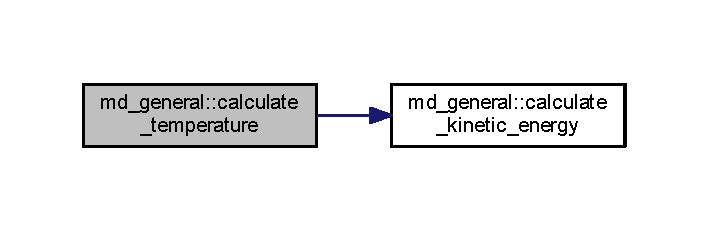
\includegraphics[width=340pt]{namespacemd__general_a1de2d09f44a8dc5b96fc5eb221845cc1_cgraph}
\end{center}
\end{figure}
\mbox{\Hypertarget{namespacemd__general_a5614c27d83ed003aa01d3be2f1b45c57}\label{namespacemd__general_a5614c27d83ed003aa01d3be2f1b45c57}} 
\index{md\+\_\+general@{md\+\_\+general}!change\+\_\+particle\+\_\+group\+\_\+n@{change\+\_\+particle\+\_\+group\+\_\+n}}
\index{change\+\_\+particle\+\_\+group\+\_\+n@{change\+\_\+particle\+\_\+group\+\_\+n}!md\+\_\+general@{md\+\_\+general}}
\subsubsection{\texorpdfstring{change\+\_\+particle\+\_\+group\+\_\+n()}{change\_particle\_group\_n()}}
{\footnotesize\ttfamily subroutine md\+\_\+general\+::change\+\_\+particle\+\_\+group\+\_\+n (\begin{DoxyParamCaption}\item[{type(\mbox{\hyperlink{structmd__general_1_1particle__group}{particle\+\_\+group}})}]{group,  }\item[{integer}]{md\+\_\+step,  }\item[{integer}]{change\+\_\+ts1,  }\item[{integer}]{change\+\_\+ts2,  }\item[{integer}]{change\+\_\+frec,  }\item[{type(\mbox{\hyperlink{structmd__general_1_1particle__group}{particle\+\_\+group}})}]{init\+\_\+group }\end{DoxyParamCaption})}



См. определение в файле md\+\_\+general.\+f90 строка 83


\begin{DoxyCode}
83     \textcolor{keywordtype}{type}(particle\_group)::  group,init\_group
84     \textcolor{keywordtype}{integer}:: md\_step,change\_ts1,change\_ts2,change\_frec
85 
86     \textcolor{keywordflow}{if}(md\_step<=change\_ts1) \textcolor{keywordflow}{then}
87         group%N = init\_group%N
88         \textcolor{keywordflow}{if}(md\_step==change\_ts1) group%N = group%N+1
89     \textcolor{keywordflow}{else}
90         \textcolor{keywordflow}{if}(md\_step<change\_ts2 .and. mod(md\_step-change\_ts1,change\_frec)==0) group%N = group%N+1
91 \textcolor{keywordflow}{    endif}
92     \textcolor{keywordflow}{if}(group%N>\textcolor{keyword}{size}(group%indexes)) group%N = \textcolor{keyword}{size}(group%indexes)
93     
\end{DoxyCode}
\mbox{\Hypertarget{namespacemd__general_ac9e62480edf60d2b3d1a123c9da68e1f}\label{namespacemd__general_ac9e62480edf60d2b3d1a123c9da68e1f}} 
\index{md\+\_\+general@{md\+\_\+general}!check\+\_\+positions@{check\+\_\+positions}}
\index{check\+\_\+positions@{check\+\_\+positions}!md\+\_\+general@{md\+\_\+general}}
\subsubsection{\texorpdfstring{check\+\_\+positions()}{check\_positions()}}
{\footnotesize\ttfamily subroutine md\+\_\+general\+::check\+\_\+positions (\begin{DoxyParamCaption}\item[{integer}]{out\+\_\+id,  }\item[{type(\mbox{\hyperlink{structmd__general_1_1particles}{particles}})}]{atoms,  }\item[{type(\mbox{\hyperlink{structmd__general_1_1simulation__cell}{simulation\+\_\+cell}})}]{box }\end{DoxyParamCaption})}



См. определение в файле md\+\_\+general.\+f90 строка 327


\begin{DoxyCode}
327     \textcolor{keywordtype}{type}(particles)::   atoms
328     \textcolor{keywordtype}{type}(simulation\_cell):: box
329     \textcolor{keywordtype}{integer}:: out\_id,i,k,p
330     \textcolor{keywordtype}{real}:: tolerance=0.0000001
331     
332     \textcolor{comment}{!$OMP PARALLEL private(i,k,p)}
333     p=0
334     \textcolor{comment}{!$OMP DO}
335     \textcolor{keywordflow}{do} i=1,atoms%N
336         \textcolor{keywordflow}{do} k=1,3
337             \textcolor{keywordflow}{if}( .not.(atoms%positions(k,i)>(0.-tolerance) .and. atoms%positions(k,i)<(box%box\_size(k)+
      tolerance)) ) \textcolor{keywordflow}{then}
338                 \textcolor{keyword}{write}(out\_id,*) i,\textcolor{stringliteral}{' particle out of cell '},atoms%positions(:,i)
339                 p = p+1
340 \textcolor{keywordflow}{            endif}
341 \textcolor{keywordflow}{        enddo}
342 \textcolor{keywordflow}{    enddo}
343     \textcolor{comment}{!$OMP END DO}
344     \textcolor{comment}{!$OMP BARRIER}
345     \textcolor{keywordflow}{if}(p>0) stop
346     \textcolor{comment}{!$OMP END PARALLEL}
347     
\end{DoxyCode}
\mbox{\Hypertarget{namespacemd__general_abd425450c2140a07748c79f0f0dbd760}\label{namespacemd__general_abd425450c2140a07748c79f0f0dbd760}} 
\index{md\+\_\+general@{md\+\_\+general}!check\+\_\+velocities@{check\+\_\+velocities}}
\index{check\+\_\+velocities@{check\+\_\+velocities}!md\+\_\+general@{md\+\_\+general}}
\subsubsection{\texorpdfstring{check\+\_\+velocities()}{check\_velocities()}}
{\footnotesize\ttfamily subroutine md\+\_\+general\+::check\+\_\+velocities (\begin{DoxyParamCaption}\item[{integer}]{out\+\_\+id,  }\item[{type(\mbox{\hyperlink{structmd__general_1_1particles}{particles}})}]{atoms }\end{DoxyParamCaption})}



См. определение в файле md\+\_\+general.\+f90 строка 351


\begin{DoxyCode}
351     \textcolor{keywordtype}{type}(particles)::   atoms
352     \textcolor{keywordtype}{integer}:: out\_id,i
353     \textcolor{keywordtype}{real}:: maxvel2,v2
354 
355     maxvel2 = -1.   
356     \textcolor{comment}{!$OMP PARALLEL DO private(i,v2) REDUCTION(max:maxvel2)}
357     \textcolor{keywordflow}{do} i=1,atoms%N
358         v2 = sum(atoms%velocities(:,i)**2)
359         \textcolor{keywordflow}{if}(maxvel2<v2) maxvel2 = v2
360 \textcolor{keywordflow}{    enddo}
361     \textcolor{comment}{!$OMP END PARALLEL DO}
362     \textcolor{keyword}{write}(out\_id,\textcolor{stringliteral}{'(A,f16.8,A)'}) \textcolor{stringliteral}{' max velocity: '},sqrt(maxvel2),\textcolor{stringliteral}{' A/fs '}
363     
\end{DoxyCode}
\mbox{\Hypertarget{namespacemd__general_a6e847bdd3b7115bf5ff69e8cd8e68d7f}\label{namespacemd__general_a6e847bdd3b7115bf5ff69e8cd8e68d7f}} 
\index{md\+\_\+general@{md\+\_\+general}!create\+\_\+particle\+\_\+group@{create\+\_\+particle\+\_\+group}}
\index{create\+\_\+particle\+\_\+group@{create\+\_\+particle\+\_\+group}!md\+\_\+general@{md\+\_\+general}}
\subsubsection{\texorpdfstring{create\+\_\+particle\+\_\+group()}{create\_particle\_group()}}
{\footnotesize\ttfamily subroutine md\+\_\+general\+::create\+\_\+particle\+\_\+group (\begin{DoxyParamCaption}\item[{type(\mbox{\hyperlink{structmd__general_1_1particle__group}{particle\+\_\+group}})}]{group,  }\item[{character(len=32), dimension(\+:)}]{type\+\_\+names,  }\item[{type(\mbox{\hyperlink{structmd__general_1_1particles}{particles}})}]{atoms }\end{DoxyParamCaption})}



См. определение в файле md\+\_\+general.\+f90 строка 58


\begin{DoxyCode}
58     \textcolor{keywordtype}{type}(particles)::   atoms
59     \textcolor{keywordtype}{type}(particle\_group)::  group
60     \textcolor{keywordtype}{character(len=32)}:: type\_names(:)
61     \textcolor{keywordtype}{integer}:: i,j,ind
62 
63     group%N = 0
64     \textcolor{keywordflow}{do} j=1,\textcolor{keyword}{size}(type\_names)
65         group%N = group%N+count(atoms%atom\_types==type\_names(j))
66 \textcolor{keywordflow}{    enddo}
67     \textcolor{keyword}{allocate}(group%indexes(group%N))
68 
69     ind=0
70     \textcolor{keywordflow}{do} j=1,\textcolor{keyword}{size}(type\_names)
71         \textcolor{keywordflow}{do} i=1,atoms%N
72             \textcolor{keywordflow}{if} (atoms%atom\_types(i)==type\_names(j)) \textcolor{keywordflow}{then}
73                 ind=ind+1
74                 group%indexes(ind) = i
75 \textcolor{keywordflow}{            endif}
76 \textcolor{keywordflow}{        enddo}
77 \textcolor{keywordflow}{    enddo}
78 
79     \textcolor{keywordflow}{return}
\end{DoxyCode}
\mbox{\Hypertarget{namespacemd__general_a33570f37733690b0634f039ad1bcf35e}\label{namespacemd__general_a33570f37733690b0634f039ad1bcf35e}} 
\index{md\+\_\+general@{md\+\_\+general}!find\+\_\+distance@{find\+\_\+distance}}
\index{find\+\_\+distance@{find\+\_\+distance}!md\+\_\+general@{md\+\_\+general}}
\subsubsection{\texorpdfstring{find\+\_\+distance()}{find\_distance()}}
{\footnotesize\ttfamily pure subroutine md\+\_\+general\+::find\+\_\+distance (\begin{DoxyParamCaption}\item[{real, dimension(3), intent(out)}]{dr,  }\item[{real, intent(out)}]{dr2,  }\item[{real, dimension(3), intent(in)}]{vec1,  }\item[{real, dimension(3), intent(in)}]{vec2,  }\item[{type(\mbox{\hyperlink{structmd__general_1_1simulation__cell}{simulation\+\_\+cell}}), intent(in)}]{box }\end{DoxyParamCaption})}



См. определение в файле md\+\_\+general.\+f90 строка 408


\begin{DoxyCode}
408     \textcolor{keywordtype}{type}(simulation\_cell), \textcolor{keywordtype}{intent (in)} :: box
409     \textcolor{keywordtype}{real}, \textcolor{keywordtype}{intent (in)} :: vec1(3),vec2(3)
410     \textcolor{keywordtype}{real}, \textcolor{keywordtype}{intent (out)} :: dr(3),dr2
411 
412     dr(1) = vec2(1)-vec1(1)
413     dr(2) = vec2(2)-vec1(2)
414     dr(3) = vec2(3)-vec1(3)
415     dr(1) = dr(1)-box%half\_box\_size(1)*(sign(1.,dr(1)-box%half\_box\_size(1))+sign(1.,dr(1)+box%half\_box\_size
      (1)))
416     dr(2) = dr(2)-box%half\_box\_size(2)*(sign(1.,dr(2)-box%half\_box\_size(2))+sign(1.,dr(2)+box%half\_box\_size
      (2)))
417     dr(3) = dr(3)-box%half\_box\_size(3)*(sign(1.,dr(3)-box%half\_box\_size(3))+sign(1.,dr(3)+box%half\_box\_size
      (3)))
418     dr2 = dr(1)*dr(1)+dr(2)*dr(2)+dr(3)*dr(3)
419     
420     \textcolor{keywordflow}{return}
\end{DoxyCode}
\mbox{\Hypertarget{namespacemd__general_a3a69c40fe5a6e7938d398f803b21e474}\label{namespacemd__general_a3a69c40fe5a6e7938d398f803b21e474}} 
\index{md\+\_\+general@{md\+\_\+general}!init\+\_\+time\+\_\+steps@{init\+\_\+time\+\_\+steps}}
\index{init\+\_\+time\+\_\+steps@{init\+\_\+time\+\_\+steps}!md\+\_\+general@{md\+\_\+general}}
\subsubsection{\texorpdfstring{init\+\_\+time\+\_\+steps()}{init\_time\_steps()}}
{\footnotesize\ttfamily subroutine md\+\_\+general\+::init\+\_\+time\+\_\+steps (\begin{DoxyParamCaption}\item[{type(\mbox{\hyperlink{structmd__general_1_1time__steps}{time\+\_\+steps}})}]{dt,  }\item[{real}]{delta\+\_\+t }\end{DoxyParamCaption})}



См. определение в файле md\+\_\+general.\+f90 строка 46


\begin{DoxyCode}
46     \textcolor{keywordtype}{type}(time\_steps):: dt
47     \textcolor{keywordtype}{integer}:: i
48     \textcolor{keywordtype}{real}::  delta\_t
49 
50     \textcolor{keywordflow}{do} i=1,\textcolor{keyword}{size}(dt%ts)
51         dt%ts(i) = delta\_t/2**(i-1)
52 \textcolor{keywordflow}{    enddo}
53 
54     \textcolor{keywordflow}{return}
\end{DoxyCode}
\mbox{\Hypertarget{namespacemd__general_aca48dc12ea3fb99991acd82c2223a9bf}\label{namespacemd__general_aca48dc12ea3fb99991acd82c2223a9bf}} 
\index{md\+\_\+general@{md\+\_\+general}!invert\+\_\+z\+\_\+velocities@{invert\+\_\+z\+\_\+velocities}}
\index{invert\+\_\+z\+\_\+velocities@{invert\+\_\+z\+\_\+velocities}!md\+\_\+general@{md\+\_\+general}}
\subsubsection{\texorpdfstring{invert\+\_\+z\+\_\+velocities()}{invert\_z\_velocities()}}
{\footnotesize\ttfamily subroutine md\+\_\+general\+::invert\+\_\+z\+\_\+velocities (\begin{DoxyParamCaption}\item[{type(\mbox{\hyperlink{structmd__general_1_1particles}{particles}})}]{atoms,  }\item[{real}]{z\+\_\+low\+\_\+border,  }\item[{real}]{z\+\_\+high\+\_\+border }\end{DoxyParamCaption})}



См. определение в файле md\+\_\+general.\+f90 строка 367


\begin{DoxyCode}
367     \textcolor{keywordtype}{type}(particles)::   atoms
368     \textcolor{keywordtype}{integer}:: i
369     \textcolor{keywordtype}{real}:: z\_low\_border,z\_high\_border
370 
371     \textcolor{comment}{!$OMP PARALLEL DO private(i)}
372     \textcolor{keywordflow}{do} i=1,atoms%N
373         \textcolor{keywordflow}{if}( (atoms%positions(3,i)>z\_low\_border .and.&
374             atoms%positions(3,i)<(z\_low\_border+z\_high\_border)/2 .and.&
375             atoms%velocities(3,i)>0.) .or.&
376             (atoms%positions(3,i)<z\_high\_border .and.&
377             atoms%positions(3,i)>(z\_low\_border+z\_high\_border)/2 .and.&
378             atoms%velocities(3,i)<0.)   )   atoms%velocities(3,i) = -atoms%velocities(3,i)
379 \textcolor{keywordflow}{    enddo}
380     \textcolor{comment}{!$OMP END PARALLEL DO}
381     
\end{DoxyCode}
\mbox{\Hypertarget{namespacemd__general_a5dc45690a2125a86ce58d01601ebdf45}\label{namespacemd__general_a5dc45690a2125a86ce58d01601ebdf45}} 
\index{md\+\_\+general@{md\+\_\+general}!position\+\_\+analysis@{position\+\_\+analysis}}
\index{position\+\_\+analysis@{position\+\_\+analysis}!md\+\_\+general@{md\+\_\+general}}
\subsubsection{\texorpdfstring{position\+\_\+analysis()}{position\_analysis()}}
{\footnotesize\ttfamily subroutine md\+\_\+general\+::position\+\_\+analysis (\begin{DoxyParamCaption}\item[{real}]{av,  }\item[{real}]{mi,  }\item[{real}]{ma,  }\item[{type(\mbox{\hyperlink{structmd__general_1_1particles}{particles}})}]{atoms,  }\item[{type(\mbox{\hyperlink{structmd__general_1_1particle__group}{particle\+\_\+group}})}]{group,  }\item[{integer}]{direction,  }\item[{real}]{minimum,  }\item[{real}]{maximum }\end{DoxyParamCaption})}



См. определение в файле md\+\_\+general.\+f90 строка 385


\begin{DoxyCode}
385     \textcolor{keywordtype}{type}(particles)::   atoms
386     \textcolor{keywordtype}{type}(particle\_group):: group
387     \textcolor{keywordtype}{real}:: minimum,maximum,av,mi,ma
388     \textcolor{keywordtype}{integer}::       i,ind,direction,k
389     
390     k = 0
391     av = 0.
392     mi = maximum
393     ma = minimum
394     \textcolor{keywordflow}{do} ind=1,group%N
395         i = group%indexes(ind)
396         \textcolor{keywordflow}{if} (atoms%positions(direction,i)<maximum .and. atoms%positions(direction,i)>minimum) \textcolor{keywordflow}{then}
397             av = av+atoms%positions(direction,i)
398             k = k+1
399             \textcolor{keywordflow}{if} (atoms%positions(direction,i)>ma) ma = atoms%positions(direction,i)
400             \textcolor{keywordflow}{if} (atoms%positions(direction,i)<mi) mi = atoms%positions(direction,i)
401 \textcolor{keywordflow}{        endif}
402 \textcolor{keywordflow}{    enddo}
403     av = av/k
404     
\end{DoxyCode}
\mbox{\Hypertarget{namespacemd__general_a8192b37ec3462b5fcb7fabf17c8eb658}\label{namespacemd__general_a8192b37ec3462b5fcb7fabf17c8eb658}} 
\index{md\+\_\+general@{md\+\_\+general}!random\+\_\+momenta@{random\+\_\+momenta}}
\index{random\+\_\+momenta@{random\+\_\+momenta}!md\+\_\+general@{md\+\_\+general}}
\subsubsection{\texorpdfstring{random\+\_\+momenta()}{random\_momenta()}}
{\footnotesize\ttfamily subroutine md\+\_\+general\+::random\+\_\+momenta (\begin{DoxyParamCaption}\item[{type(\mbox{\hyperlink{structmd__general_1_1particles}{particles}})}]{atoms,  }\item[{type(\mbox{\hyperlink{structmd__general_1_1particle__group}{particle\+\_\+group}})}]{group }\end{DoxyParamCaption})}



См. определение в файле md\+\_\+general.\+f90 строка 143


\begin{DoxyCode}
143     \textcolor{keywordtype}{type}(particles)::   atoms
144     \textcolor{keywordtype}{type}(particle\_group):: group
145     \textcolor{keywordtype}{real},\textcolor{keywordtype}{parameter}:: coef = 1.3806488/1.6605389217*10.**(-6)
146     \textcolor{keywordtype}{integer}::       i,ind
147 
148     \textcolor{keyword}{call }random\_velocities(atoms,group)
149 
150     \textcolor{comment}{!$OMP PARALLEL firstprivate(i,ind)}
151     \textcolor{comment}{!$OMP DO}
152     \textcolor{keywordflow}{do} ind=1,group%N
153         i = group%indexes(ind)
154         atoms%velocities(:,i) = atoms%velocities(:,i)*sqrt(coef/atoms%masses(i))
155 \textcolor{keywordflow}{    enddo}
156     \textcolor{comment}{!$OMP END DO}
157     \textcolor{comment}{!$OMP END PARALLEL}
158 
159     \textcolor{keywordflow}{return}
\end{DoxyCode}
Граф вызовов\+:\nopagebreak
\begin{figure}[H]
\begin{center}
\leavevmode
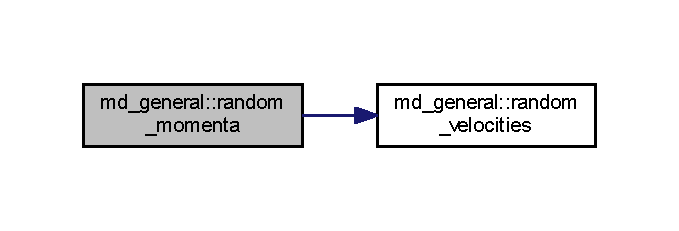
\includegraphics[width=326pt]{namespacemd__general_a8192b37ec3462b5fcb7fabf17c8eb658_cgraph}
\end{center}
\end{figure}
\mbox{\Hypertarget{namespacemd__general_a326a2fe1c1da84197c4566801133648a}\label{namespacemd__general_a326a2fe1c1da84197c4566801133648a}} 
\index{md\+\_\+general@{md\+\_\+general}!random\+\_\+velocities@{random\+\_\+velocities}}
\index{random\+\_\+velocities@{random\+\_\+velocities}!md\+\_\+general@{md\+\_\+general}}
\subsubsection{\texorpdfstring{random\+\_\+velocities()}{random\_velocities()}}
{\footnotesize\ttfamily subroutine md\+\_\+general\+::random\+\_\+velocities (\begin{DoxyParamCaption}\item[{type(\mbox{\hyperlink{structmd__general_1_1particles}{particles}})}]{atoms,  }\item[{type(\mbox{\hyperlink{structmd__general_1_1particle__group}{particle\+\_\+group}})}]{group }\end{DoxyParamCaption})}



См. определение в файле md\+\_\+general.\+f90 строка 115


\begin{DoxyCode}
115     \textcolor{keywordtype}{type}(particles)::   atoms
116     \textcolor{keywordtype}{type}(particle\_group):: group
117     \textcolor{keywordtype}{real} a1,a2,b
118     \textcolor{keywordtype}{integer}::       i,k,ind
119     \textcolor{keywordtype}{integer} omp\_get\_thread\_num
120     
121     \textcolor{comment}{!$OMP PARALLEL firstprivate(i,ind,k,a1,a2,b)}
122     \textcolor{keyword}{call }srand(omp\_get\_thread\_num())
123     \textcolor{comment}{!$OMP DO}
124     \textcolor{keywordflow}{do} ind=1,group%N
125         i = group%indexes(ind)
126         \textcolor{keywordflow}{do} k=1,3,1
127             b = 2.
128             \textcolor{keywordflow}{do} \textcolor{keywordflow}{while} (b>=1.)
129                 a1 = 2.*rand()-1.
130                 a2 = 2.*rand()-1.
131                 b = a1**2+a2**2
132 \textcolor{keywordflow}{            enddo}
133             atoms%velocities(k,i) = a1*sqrt(-2.*log(b)/b)
134 \textcolor{keywordflow}{        enddo}
135 \textcolor{keywordflow}{    enddo}
136     \textcolor{comment}{!$OMP END DO}
137     \textcolor{comment}{!$OMP END PARALLEL}
138 
139     \textcolor{keywordflow}{return}
\end{DoxyCode}
\mbox{\Hypertarget{namespacemd__general_ad4ad26fa9584c63f846d49033ce92987}\label{namespacemd__general_ad4ad26fa9584c63f846d49033ce92987}} 
\index{md\+\_\+general@{md\+\_\+general}!scale\+\_\+velocities@{scale\+\_\+velocities}}
\index{scale\+\_\+velocities@{scale\+\_\+velocities}!md\+\_\+general@{md\+\_\+general}}
\subsubsection{\texorpdfstring{scale\+\_\+velocities()}{scale\_velocities()}}
{\footnotesize\ttfamily subroutine md\+\_\+general\+::scale\+\_\+velocities (\begin{DoxyParamCaption}\item[{type(\mbox{\hyperlink{structmd__general_1_1particles}{particles}})}]{atoms,  }\item[{type(\mbox{\hyperlink{structmd__general_1_1particle__group}{particle\+\_\+group}})}]{group,  }\item[{real}]{s }\end{DoxyParamCaption})}



См. определение в файле md\+\_\+general.\+f90 строка 97


\begin{DoxyCode}
97     \textcolor{keywordtype}{type}(particles)::   atoms
98     \textcolor{keywordtype}{type}(particle\_group):: group
99     \textcolor{keywordtype}{real}:: s
100     \textcolor{keywordtype}{integer}::       i,ind
101 
102     \textcolor{comment}{!$OMP PARALLEL firstprivate(i,ind)}
103     \textcolor{comment}{!$OMP DO}
104     \textcolor{keywordflow}{do} ind=1,group%N
105         i = group%indexes(ind)
106         atoms%velocities(:,i) = atoms%velocities(:,i)*s
107 \textcolor{keywordflow}{    enddo}
108     \textcolor{comment}{!$OMP END DO}
109     \textcolor{comment}{!$OMP END PARALLEL}
110 
111     \textcolor{keywordflow}{return}
\end{DoxyCode}
\mbox{\Hypertarget{namespacemd__general_a9f99fa4920c9047597f37b777dd44b3c}\label{namespacemd__general_a9f99fa4920c9047597f37b777dd44b3c}} 
\index{md\+\_\+general@{md\+\_\+general}!set\+\_\+new\+\_\+temperature@{set\+\_\+new\+\_\+temperature}}
\index{set\+\_\+new\+\_\+temperature@{set\+\_\+new\+\_\+temperature}!md\+\_\+general@{md\+\_\+general}}
\subsubsection{\texorpdfstring{set\+\_\+new\+\_\+temperature()}{set\_new\_temperature()}}
{\footnotesize\ttfamily subroutine md\+\_\+general\+::set\+\_\+new\+\_\+temperature (\begin{DoxyParamCaption}\item[{type(\mbox{\hyperlink{structmd__general_1_1particles}{particles}})}]{atoms,  }\item[{type(\mbox{\hyperlink{structmd__general_1_1particle__group}{particle\+\_\+group}})}]{group,  }\item[{real}]{temp }\end{DoxyParamCaption})}



См. определение в файле md\+\_\+general.\+f90 строка 315


\begin{DoxyCode}
315     \textcolor{keywordtype}{type}(particles)::   atoms
316     \textcolor{keywordtype}{type}(particle\_group):: group
317     \textcolor{keywordtype}{real}:: temp,ke,temperature
318     
319     \textcolor{keyword}{call }random\_momenta(atoms,group)
320     \textcolor{keyword}{call }zero\_momentum(atoms,group)
321     \textcolor{keyword}{call }calculate\_temperature(temperature,ke,atoms,group)
322     \textcolor{keyword}{call }scale\_velocities(atoms,group,sqrt(temp/temperature))
323 
\end{DoxyCode}
Граф вызовов\+:\nopagebreak
\begin{figure}[H]
\begin{center}
\leavevmode
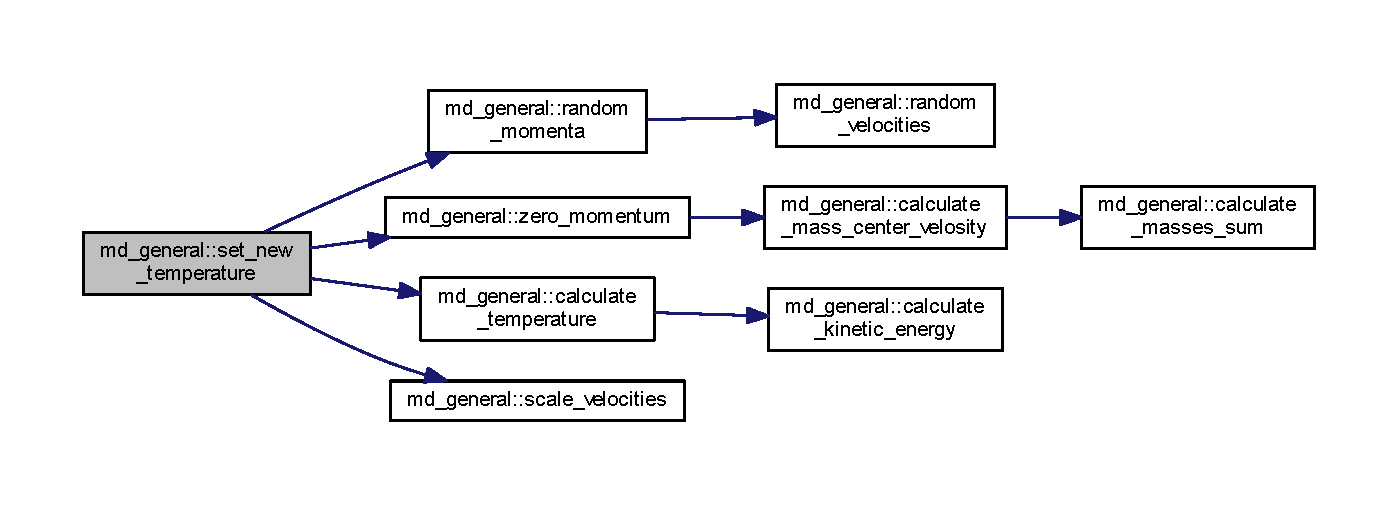
\includegraphics[width=350pt]{namespacemd__general_a9f99fa4920c9047597f37b777dd44b3c_cgraph}
\end{center}
\end{figure}
\mbox{\Hypertarget{namespacemd__general_a79ea9e512a27c651278559e30f97a336}\label{namespacemd__general_a79ea9e512a27c651278559e30f97a336}} 
\index{md\+\_\+general@{md\+\_\+general}!zero\+\_\+momentum@{zero\+\_\+momentum}}
\index{zero\+\_\+momentum@{zero\+\_\+momentum}!md\+\_\+general@{md\+\_\+general}}
\subsubsection{\texorpdfstring{zero\+\_\+momentum()}{zero\_momentum()}}
{\footnotesize\ttfamily subroutine md\+\_\+general\+::zero\+\_\+momentum (\begin{DoxyParamCaption}\item[{type(\mbox{\hyperlink{structmd__general_1_1particles}{particles}})}]{atoms,  }\item[{type(\mbox{\hyperlink{structmd__general_1_1particle__group}{particle\+\_\+group}})}]{group }\end{DoxyParamCaption})}



См. определение в файле md\+\_\+general.\+f90 строка 238


\begin{DoxyCode}
238     \textcolor{keywordtype}{type}(particles)::   atoms
239     \textcolor{keywordtype}{type}(particle\_group):: group
240     \textcolor{keywordtype}{integer}::       i,ind
241     \textcolor{keywordtype}{real}:: mcv(3)
242     
243     \textcolor{keyword}{call }calculate\_mass\_center\_velosity(mcv,atoms,group)
244     \textcolor{comment}{!$OMP PARALLEL firstprivate(mcv,i,ind)}
245     \textcolor{comment}{!$OMP DO}
246     \textcolor{keywordflow}{do} ind=1,group%N
247         i = group%indexes(ind)
248         atoms%velocities(:,i) = atoms%velocities(:,i)-mcv
249 \textcolor{keywordflow}{    enddo}
250     \textcolor{comment}{!$OMP END DO}
251     \textcolor{comment}{!$OMP END PARALLEL}
252     
253     \textcolor{keywordflow}{return}
\end{DoxyCode}
Граф вызовов\+:\nopagebreak
\begin{figure}[H]
\begin{center}
\leavevmode
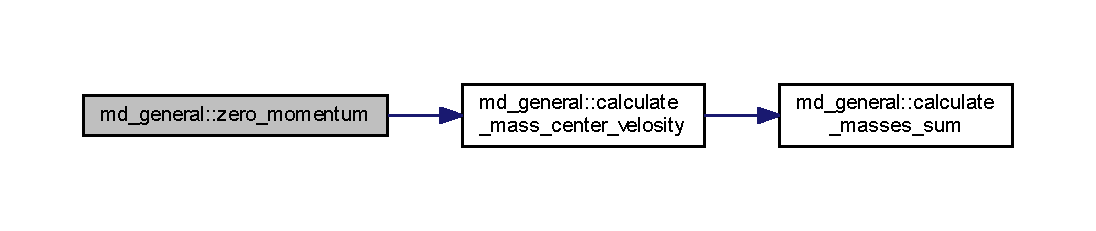
\includegraphics[width=350pt]{namespacemd__general_a79ea9e512a27c651278559e30f97a336_cgraph}
\end{center}
\end{figure}

\hypertarget{namespacemd__integrators}{}\section{Модуль md\+\_\+integrators}
\label{namespacemd__integrators}\index{md\+\_\+integrators@{md\+\_\+integrators}}
\subsection*{Функции/подпрограммы}
\begin{DoxyCompactItemize}
\item 
subroutine \mbox{\hyperlink{namespacemd__integrators_a46897b8968c1901883654589ef731eb2}{integrate\+\_\+verlet\+\_\+xyz\+\_\+positions}} (atoms, group, steps, box)
\item 
subroutine \mbox{\hyperlink{namespacemd__integrators_a89e015a65c39454223a09736f095aef0}{integrate\+\_\+verlet\+\_\+z\+\_\+positions}} (atoms, group, steps, box)
\item 
subroutine \mbox{\hyperlink{namespacemd__integrators_a4aafa379de6ec22530aa0c426855689e}{integrate\+\_\+verlet\+\_\+xyz\+\_\+velocities}} (atoms, group, steps)
\item 
subroutine \mbox{\hyperlink{namespacemd__integrators_ab71be6f8ca48e91d1a0e84d70b3176ac}{integrate\+\_\+verlet\+\_\+z\+\_\+velocities}} (atoms, group, steps)
\item 
subroutine \mbox{\hyperlink{namespacemd__integrators_a37c12502ddb5537b8b963074dcd33132}{molecular\+\_\+static\+\_\+xyz\+\_\+velocities}} (atoms, group)
\item 
subroutine \mbox{\hyperlink{namespacemd__integrators_aa4c7e5a4cfdd19fa542fccae43e9d35a}{molecular\+\_\+static\+\_\+1d\+\_\+velocities}} (atoms, group)
\item 
subroutine \mbox{\hyperlink{namespacemd__integrators_afaf5cf45b5c0a8363d40dc012c954a1a}{zero\+\_\+forces}} (atoms, group)
\item 
subroutine \mbox{\hyperlink{namespacemd__integrators_aa74788b2d003c16024b8eb999ea01c3c}{create\+\_\+nose\+\_\+hoover\+\_\+chain}} (nhc)
\item 
subroutine \mbox{\hyperlink{namespacemd__integrators_a20d655980db9ce88983d738fc91ff021}{set\+\_\+nose\+\_\+hoover\+\_\+chain}} (nhc, temp, q1, l)
\item 
subroutine \mbox{\hyperlink{namespacemd__integrators_a769781abbe7ac3aaacf761d6321d4722}{integrate\+\_\+nose\+\_\+hoover\+\_\+chain}} (nhc, atoms, group, dt)
\item 
subroutine \mbox{\hyperlink{namespacemd__integrators_a67084641a81f648ac71c15c20428c015}{calculate\+\_\+nose\+\_\+hoover\+\_\+chain\+\_\+energy}} (nhc)
\end{DoxyCompactItemize}


\subsection{Функции/подпрограммы}
\mbox{\Hypertarget{namespacemd__integrators_a67084641a81f648ac71c15c20428c015}\label{namespacemd__integrators_a67084641a81f648ac71c15c20428c015}} 
\index{md\+\_\+integrators@{md\+\_\+integrators}!calculate\+\_\+nose\+\_\+hoover\+\_\+chain\+\_\+energy@{calculate\+\_\+nose\+\_\+hoover\+\_\+chain\+\_\+energy}}
\index{calculate\+\_\+nose\+\_\+hoover\+\_\+chain\+\_\+energy@{calculate\+\_\+nose\+\_\+hoover\+\_\+chain\+\_\+energy}!md\+\_\+integrators@{md\+\_\+integrators}}
\subsubsection{\texorpdfstring{calculate\+\_\+nose\+\_\+hoover\+\_\+chain\+\_\+energy()}{calculate\_nose\_hoover\_chain\_energy()}}
{\footnotesize\ttfamily subroutine md\+\_\+integrators\+::calculate\+\_\+nose\+\_\+hoover\+\_\+chain\+\_\+energy (\begin{DoxyParamCaption}\item[{type(\mbox{\hyperlink{structmd__general_1_1nose__hoover__chain}{nose\+\_\+hoover\+\_\+chain}})}]{nhc }\end{DoxyParamCaption})}



См. определение в файле md\+\_\+integrators.\+f90 строка 242


\begin{DoxyCode}
242     \textcolor{keywordtype}{type}(nose\_hoover\_chain):: nhc
243     \textcolor{keywordtype}{real}:: kt
244     \textcolor{keywordtype}{integer}::       i
245 
246     kt=1.3806488/1.6021765654*10.**(-4)*nhc%temperature
247 
248     nhc%e = nhc%q(1)/2*nhc%v(1)**2+3.*nhc%L*kt*nhc%x(1)
249     \textcolor{keywordflow}{do} i=2,nhc%M,1
250         nhc%e = nhc%e+nhc%q(i)/2*nhc%v(i)**2+kt*nhc%x(i)
251 \textcolor{keywordflow}{    enddo}
252 
253     \textcolor{keywordflow}{return}
\end{DoxyCode}
\mbox{\Hypertarget{namespacemd__integrators_aa74788b2d003c16024b8eb999ea01c3c}\label{namespacemd__integrators_aa74788b2d003c16024b8eb999ea01c3c}} 
\index{md\+\_\+integrators@{md\+\_\+integrators}!create\+\_\+nose\+\_\+hoover\+\_\+chain@{create\+\_\+nose\+\_\+hoover\+\_\+chain}}
\index{create\+\_\+nose\+\_\+hoover\+\_\+chain@{create\+\_\+nose\+\_\+hoover\+\_\+chain}!md\+\_\+integrators@{md\+\_\+integrators}}
\subsubsection{\texorpdfstring{create\+\_\+nose\+\_\+hoover\+\_\+chain()}{create\_nose\_hoover\_chain()}}
{\footnotesize\ttfamily subroutine md\+\_\+integrators\+::create\+\_\+nose\+\_\+hoover\+\_\+chain (\begin{DoxyParamCaption}\item[{type(\mbox{\hyperlink{structmd__general_1_1nose__hoover__chain}{nose\+\_\+hoover\+\_\+chain}})}]{nhc }\end{DoxyParamCaption})}



См. определение в файле md\+\_\+integrators.\+f90 строка 167


\begin{DoxyCode}
167     \textcolor{keywordtype}{type}(nose\_hoover\_chain):: nhc
168 
169     \textcolor{keyword}{allocate}(nhc%x(nhc%M))
170     \textcolor{keyword}{allocate}(nhc%v(nhc%M))
171     \textcolor{keyword}{allocate}(nhc%q(nhc%M))
172     nhc%x = 0.
173     nhc%v = 0.
174     nhc%q = 0.
175     nhc%e = 0.
176     nhc%s = 1.
177 
178     \textcolor{keywordflow}{return}
\end{DoxyCode}
\mbox{\Hypertarget{namespacemd__integrators_a769781abbe7ac3aaacf761d6321d4722}\label{namespacemd__integrators_a769781abbe7ac3aaacf761d6321d4722}} 
\index{md\+\_\+integrators@{md\+\_\+integrators}!integrate\+\_\+nose\+\_\+hoover\+\_\+chain@{integrate\+\_\+nose\+\_\+hoover\+\_\+chain}}
\index{integrate\+\_\+nose\+\_\+hoover\+\_\+chain@{integrate\+\_\+nose\+\_\+hoover\+\_\+chain}!md\+\_\+integrators@{md\+\_\+integrators}}
\subsubsection{\texorpdfstring{integrate\+\_\+nose\+\_\+hoover\+\_\+chain()}{integrate\_nose\_hoover\_chain()}}
{\footnotesize\ttfamily subroutine md\+\_\+integrators\+::integrate\+\_\+nose\+\_\+hoover\+\_\+chain (\begin{DoxyParamCaption}\item[{type(\mbox{\hyperlink{structmd__general_1_1nose__hoover__chain}{nose\+\_\+hoover\+\_\+chain}})}]{nhc,  }\item[{type(\mbox{\hyperlink{structmd__general_1_1particles}{particles}})}]{atoms,  }\item[{type(\mbox{\hyperlink{structmd__general_1_1particle__group}{particle\+\_\+group}})}]{group,  }\item[{type(\mbox{\hyperlink{structmd__general_1_1time__steps}{time\+\_\+steps}})}]{dt }\end{DoxyParamCaption})}



См. определение в файле md\+\_\+integrators.\+f90 строка 197


\begin{DoxyCode}
197     \textcolor{keywordtype}{type}(particles)::   atoms
198     \textcolor{keywordtype}{type}(particle\_group):: group
199     \textcolor{keywordtype}{type}(time\_steps):: dt
200     \textcolor{keywordtype}{type}(nose\_hoover\_chain):: nhc
201     \textcolor{keywordtype}{real}:: kedif,ke,kt,b
202     \textcolor{keywordtype}{integer}::       i
203 
204     \textcolor{keyword}{call }calculate\_kinetic\_energy(ke,atoms,group)
205     kt=1.3806488/1.6021765654*10.**(-4)*nhc%temperature
206     kedif = 2.*ke-3.*nhc%L*kt
207 
208     \textcolor{keywordflow}{if} (nhc%M==1) \textcolor{keywordflow}{then}
209         nhc%v(1)=nhc%v(1)+kedif/nhc%q(1)*dt%ts(3)
210     \textcolor{keywordflow}{else}
211         nhc%v(nhc%M)=nhc%v(nhc%M)+(nhc%q(nhc%M-1)*nhc%v(nhc%M-1)**2-kt)/nhc%q(nhc%M)*dt%ts(3)
212         \textcolor{keywordflow}{do} i=nhc%M-1,2,-1
213             b=exp(-nhc%v(i+1)*dt%ts(4))
214             nhc%v(i)=nhc%v(i)*b**2+(nhc%q(i-1)*nhc%v(i-1)**2-kt)/nhc%q(i)*dt%ts(3)*b
215 \textcolor{keywordflow}{        enddo}
216         b=exp(-nhc%v(2)*dt%ts(4))
217         nhc%v(1)=nhc%v(1)*b**2+kedif/nhc%q(1)*dt%ts(3)*b
218 \textcolor{keywordflow}{    endif}
219 
220     nhc%s=exp(-nhc%v(1)*dt%ts(2))
221     \textcolor{keyword}{call }scale\_velocities(atoms,group,nhc%s)
222     kedif = 2.*ke*nhc%s**2-3.*nhc%L*kt
223     \textcolor{keywordflow}{do} i=1,nhc%M,1
224         nhc%x(i)=nhc%x(i)+nhc%v(i)*dt%ts(2)
225 \textcolor{keywordflow}{    enddo}
226 
227     \textcolor{keywordflow}{if} (nhc%M==1) \textcolor{keywordflow}{then}
228         nhc%v(1)=nhc%v(1)+kedif/nhc%q(1)*dt%ts(3)
229     \textcolor{keywordflow}{else}
230         nhc%v(1)=nhc%v(1)*b**2+kedif/nhc%q(1)*dt%ts(3)*b
231         \textcolor{keywordflow}{do} i=2,nhc%M-1,1
232             b=exp(-nhc%v(i+1)*dt%ts(4))
233             nhc%v(i)=nhc%v(i)*b**2+(nhc%q(i-1)*nhc%v(i-1)**2-kt)/nhc%q(i)*dt%ts(3)*b
234 \textcolor{keywordflow}{        enddo}
235         nhc%v(nhc%M)=nhc%v(nhc%M)+(nhc%q(nhc%M-1)*nhc%v(nhc%M-1)**2-kt)/nhc%q(nhc%M)*dt%ts(3)
236 \textcolor{keywordflow}{    endif}
237 
238     \textcolor{keywordflow}{return}
\end{DoxyCode}
Граф вызовов\+:\nopagebreak
\begin{figure}[H]
\begin{center}
\leavevmode
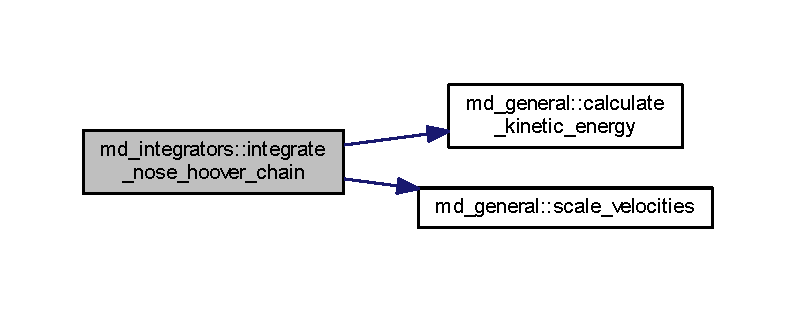
\includegraphics[width=350pt]{namespacemd__integrators_a769781abbe7ac3aaacf761d6321d4722_cgraph}
\end{center}
\end{figure}
\mbox{\Hypertarget{namespacemd__integrators_a46897b8968c1901883654589ef731eb2}\label{namespacemd__integrators_a46897b8968c1901883654589ef731eb2}} 
\index{md\+\_\+integrators@{md\+\_\+integrators}!integrate\+\_\+verlet\+\_\+xyz\+\_\+positions@{integrate\+\_\+verlet\+\_\+xyz\+\_\+positions}}
\index{integrate\+\_\+verlet\+\_\+xyz\+\_\+positions@{integrate\+\_\+verlet\+\_\+xyz\+\_\+positions}!md\+\_\+integrators@{md\+\_\+integrators}}
\subsubsection{\texorpdfstring{integrate\+\_\+verlet\+\_\+xyz\+\_\+positions()}{integrate\_verlet\_xyz\_positions()}}
{\footnotesize\ttfamily subroutine md\+\_\+integrators\+::integrate\+\_\+verlet\+\_\+xyz\+\_\+positions (\begin{DoxyParamCaption}\item[{type(\mbox{\hyperlink{structmd__general_1_1particles}{particles}})}]{atoms,  }\item[{type(\mbox{\hyperlink{structmd__general_1_1particle__group}{particle\+\_\+group}})}]{group,  }\item[{type(\mbox{\hyperlink{structmd__general_1_1time__steps}{time\+\_\+steps}})}]{steps,  }\item[{type(\mbox{\hyperlink{structmd__general_1_1simulation__cell}{simulation\+\_\+cell}})}]{box }\end{DoxyParamCaption})}



См. определение в файле md\+\_\+integrators.\+f90 строка 8


\begin{DoxyCode}
8     \textcolor{keywordtype}{type}(particles)::   atoms
9     \textcolor{keywordtype}{type}(particle\_group):: group
10     \textcolor{keywordtype}{type}(time\_steps):: steps
11     \textcolor{keywordtype}{type}(simulation\_cell):: box
12     \textcolor{keywordtype}{integer}::       i,k,ind
13 
14     \textcolor{comment}{!$OMP PARALLEL firstprivate(i,ind,k)}
15     \textcolor{comment}{!$OMP DO}
16     \textcolor{keywordflow}{do} ind=1,group%N
17         i = group%indexes(ind)
18         \textcolor{keywordflow}{do} k=1,3
19             atoms%positions(k,i) = atoms%positions(k,i)+atoms%velocities(k,i)*steps%ts(1)
20             \textcolor{keywordflow}{if} (atoms%positions(k,i)>box%box\_size(k)) \textcolor{keywordflow}{then}
21                 atoms%positions(k,i) = atoms%positions(k,i)-box%box\_size(k)
22             \textcolor{keywordflow}{elseif} (atoms%positions(k,i)<0.) \textcolor{keywordflow}{then}
23                 atoms%positions(k,i) = atoms%positions(k,i)+box%box\_size(k)
24 \textcolor{keywordflow}{            endif}
25 \textcolor{keywordflow}{        enddo}
26 \textcolor{keywordflow}{    enddo}
27     \textcolor{comment}{!$OMP END DO}
28     \textcolor{comment}{!$OMP END PARALLEL}
29 
30     \textcolor{keywordflow}{return}
\end{DoxyCode}
\mbox{\Hypertarget{namespacemd__integrators_a4aafa379de6ec22530aa0c426855689e}\label{namespacemd__integrators_a4aafa379de6ec22530aa0c426855689e}} 
\index{md\+\_\+integrators@{md\+\_\+integrators}!integrate\+\_\+verlet\+\_\+xyz\+\_\+velocities@{integrate\+\_\+verlet\+\_\+xyz\+\_\+velocities}}
\index{integrate\+\_\+verlet\+\_\+xyz\+\_\+velocities@{integrate\+\_\+verlet\+\_\+xyz\+\_\+velocities}!md\+\_\+integrators@{md\+\_\+integrators}}
\subsubsection{\texorpdfstring{integrate\+\_\+verlet\+\_\+xyz\+\_\+velocities()}{integrate\_verlet\_xyz\_velocities()}}
{\footnotesize\ttfamily subroutine md\+\_\+integrators\+::integrate\+\_\+verlet\+\_\+xyz\+\_\+velocities (\begin{DoxyParamCaption}\item[{type(\mbox{\hyperlink{structmd__general_1_1particles}{particles}})}]{atoms,  }\item[{type(\mbox{\hyperlink{structmd__general_1_1particle__group}{particle\+\_\+group}})}]{group,  }\item[{type(\mbox{\hyperlink{structmd__general_1_1time__steps}{time\+\_\+steps}})}]{steps }\end{DoxyParamCaption})}



См. определение в файле md\+\_\+integrators.\+f90 строка 59


\begin{DoxyCode}
59     \textcolor{keywordtype}{type}(particles)::   atoms
60     \textcolor{keywordtype}{type}(particle\_group):: group
61     \textcolor{keywordtype}{type}(time\_steps):: steps
62     \textcolor{keywordtype}{real},\textcolor{keywordtype}{parameter}:: mass\_coef=1.6605389217/1.6021765654*10.**(2)
63     \textcolor{keywordtype}{integer}::       i,ind,k
64 
65     \textcolor{comment}{!$OMP PARALLEL firstprivate(i,ind,k)}
66     \textcolor{comment}{!$OMP DO}
67     \textcolor{keywordflow}{do} ind=1,group%N
68         i = group%indexes(ind)
69         \textcolor{keywordflow}{do} k=1,3
70             atoms%velocities(k,i) = atoms%velocities(k,i)+atoms%forces(k,i)/atoms%masses(i)/mass\_coef*steps
      %ts(2)
71 \textcolor{keywordflow}{        enddo}
72 \textcolor{keywordflow}{    enddo}
73     \textcolor{comment}{!$OMP END DO}
74     \textcolor{comment}{!$OMP END PARALLEL}
75 
76     \textcolor{keywordflow}{return}
\end{DoxyCode}
\mbox{\Hypertarget{namespacemd__integrators_a89e015a65c39454223a09736f095aef0}\label{namespacemd__integrators_a89e015a65c39454223a09736f095aef0}} 
\index{md\+\_\+integrators@{md\+\_\+integrators}!integrate\+\_\+verlet\+\_\+z\+\_\+positions@{integrate\+\_\+verlet\+\_\+z\+\_\+positions}}
\index{integrate\+\_\+verlet\+\_\+z\+\_\+positions@{integrate\+\_\+verlet\+\_\+z\+\_\+positions}!md\+\_\+integrators@{md\+\_\+integrators}}
\subsubsection{\texorpdfstring{integrate\+\_\+verlet\+\_\+z\+\_\+positions()}{integrate\_verlet\_z\_positions()}}
{\footnotesize\ttfamily subroutine md\+\_\+integrators\+::integrate\+\_\+verlet\+\_\+z\+\_\+positions (\begin{DoxyParamCaption}\item[{type(\mbox{\hyperlink{structmd__general_1_1particles}{particles}})}]{atoms,  }\item[{type(\mbox{\hyperlink{structmd__general_1_1particle__group}{particle\+\_\+group}})}]{group,  }\item[{type(\mbox{\hyperlink{structmd__general_1_1time__steps}{time\+\_\+steps}})}]{steps,  }\item[{type(\mbox{\hyperlink{structmd__general_1_1simulation__cell}{simulation\+\_\+cell}})}]{box }\end{DoxyParamCaption})}



См. определение в файле md\+\_\+integrators.\+f90 строка 34


\begin{DoxyCode}
34     \textcolor{keywordtype}{type}(particles)::   atoms
35     \textcolor{keywordtype}{type}(particle\_group):: group
36     \textcolor{keywordtype}{type}(time\_steps):: steps
37     \textcolor{keywordtype}{type}(simulation\_cell):: box
38     \textcolor{keywordtype}{integer}::       i,k,ind
39 
40     \textcolor{comment}{!$OMP PARALLEL firstprivate(i,ind,k)}
41     \textcolor{comment}{!$OMP DO}
42     \textcolor{keywordflow}{do} ind=1,group%N
43         i = group%indexes(ind)
44         k = 3
45             atoms%positions(k,i) = atoms%positions(k,i)+atoms%velocities(k,i)*steps%ts(1)
46             \textcolor{keywordflow}{if} (atoms%positions(k,i)>box%box\_size(k)) \textcolor{keywordflow}{then}
47                 atoms%positions(k,i) = atoms%positions(k,i)-box%box\_size(k)
48             \textcolor{keywordflow}{elseif} (atoms%positions(k,i)<0.) \textcolor{keywordflow}{then}
49                 atoms%positions(k,i) = atoms%positions(k,i)+box%box\_size(k)
50 \textcolor{keywordflow}{            endif}
51 \textcolor{keywordflow}{    enddo}
52     \textcolor{comment}{!$OMP END DO}
53     \textcolor{comment}{!$OMP END PARALLEL}
54 
55     \textcolor{keywordflow}{return}
\end{DoxyCode}
\mbox{\Hypertarget{namespacemd__integrators_ab71be6f8ca48e91d1a0e84d70b3176ac}\label{namespacemd__integrators_ab71be6f8ca48e91d1a0e84d70b3176ac}} 
\index{md\+\_\+integrators@{md\+\_\+integrators}!integrate\+\_\+verlet\+\_\+z\+\_\+velocities@{integrate\+\_\+verlet\+\_\+z\+\_\+velocities}}
\index{integrate\+\_\+verlet\+\_\+z\+\_\+velocities@{integrate\+\_\+verlet\+\_\+z\+\_\+velocities}!md\+\_\+integrators@{md\+\_\+integrators}}
\subsubsection{\texorpdfstring{integrate\+\_\+verlet\+\_\+z\+\_\+velocities()}{integrate\_verlet\_z\_velocities()}}
{\footnotesize\ttfamily subroutine md\+\_\+integrators\+::integrate\+\_\+verlet\+\_\+z\+\_\+velocities (\begin{DoxyParamCaption}\item[{type(\mbox{\hyperlink{structmd__general_1_1particles}{particles}})}]{atoms,  }\item[{type(\mbox{\hyperlink{structmd__general_1_1particle__group}{particle\+\_\+group}})}]{group,  }\item[{type(\mbox{\hyperlink{structmd__general_1_1time__steps}{time\+\_\+steps}})}]{steps }\end{DoxyParamCaption})}



См. определение в файле md\+\_\+integrators.\+f90 строка 80


\begin{DoxyCode}
80     \textcolor{keywordtype}{type}(particles)::   atoms
81     \textcolor{keywordtype}{type}(particle\_group):: group
82     \textcolor{keywordtype}{type}(time\_steps):: steps
83     \textcolor{keywordtype}{real},\textcolor{keywordtype}{parameter}:: mass\_coef=1.6605389217/1.6021765654*10.**(2)
84     \textcolor{keywordtype}{integer}::       i,ind,k
85 
86     \textcolor{comment}{!$OMP PARALLEL firstprivate(i,ind,k)}
87     \textcolor{comment}{!$OMP DO}
88     \textcolor{keywordflow}{do} ind=1,group%N
89         i = group%indexes(ind)
90         k = 3
91             atoms%velocities(k,i) = atoms%velocities(k,i)+atoms%forces(k,i)/atoms%masses(i)/mass\_coef*steps
      %ts(2)
92 \textcolor{keywordflow}{    enddo}
93     \textcolor{comment}{!$OMP END DO}
94     \textcolor{comment}{!$OMP END PARALLEL}
95 
96     \textcolor{keywordflow}{return}
\end{DoxyCode}
\mbox{\Hypertarget{namespacemd__integrators_aa4c7e5a4cfdd19fa542fccae43e9d35a}\label{namespacemd__integrators_aa4c7e5a4cfdd19fa542fccae43e9d35a}} 
\index{md\+\_\+integrators@{md\+\_\+integrators}!molecular\+\_\+static\+\_\+1d\+\_\+velocities@{molecular\+\_\+static\+\_\+1d\+\_\+velocities}}
\index{molecular\+\_\+static\+\_\+1d\+\_\+velocities@{molecular\+\_\+static\+\_\+1d\+\_\+velocities}!md\+\_\+integrators@{md\+\_\+integrators}}
\subsubsection{\texorpdfstring{molecular\+\_\+static\+\_\+1d\+\_\+velocities()}{molecular\_static\_1d\_velocities()}}
{\footnotesize\ttfamily subroutine md\+\_\+integrators\+::molecular\+\_\+static\+\_\+1d\+\_\+velocities (\begin{DoxyParamCaption}\item[{type(\mbox{\hyperlink{structmd__general_1_1particles}{particles}})}]{atoms,  }\item[{type(\mbox{\hyperlink{structmd__general_1_1particle__group}{particle\+\_\+group}})}]{group }\end{DoxyParamCaption})}



См. определение в файле md\+\_\+integrators.\+f90 строка 126


\begin{DoxyCode}
126     \textcolor{keywordtype}{type}(particles)::   atoms
127     \textcolor{keywordtype}{type}(particle\_group):: group
128     \textcolor{keywordtype}{real}:: fv
129     \textcolor{keywordtype}{integer}:: i,k,ind
130 
131     \textcolor{comment}{!$OMP PARALLEL firstprivate(i,k,ind,fv)}
132     \textcolor{comment}{!$OMP DO}
133     \textcolor{keywordflow}{do} ind=1,group%N
134         i = group%indexes(ind)
135         fv = sum(atoms%forces(:,i)*atoms%velocities(:,i))
136         \textcolor{keywordflow}{if} (fv>0.) \textcolor{keywordflow}{then}
137         \textcolor{keywordflow}{else}
138             atoms%velocities(:,i) = 0.
139 \textcolor{keywordflow}{        endif}
140 \textcolor{keywordflow}{    enddo}
141     \textcolor{comment}{!$OMP END DO}
142     \textcolor{comment}{!$OMP END PARALLEL}
143 
144     \textcolor{keywordflow}{return}
\end{DoxyCode}
\mbox{\Hypertarget{namespacemd__integrators_a37c12502ddb5537b8b963074dcd33132}\label{namespacemd__integrators_a37c12502ddb5537b8b963074dcd33132}} 
\index{md\+\_\+integrators@{md\+\_\+integrators}!molecular\+\_\+static\+\_\+xyz\+\_\+velocities@{molecular\+\_\+static\+\_\+xyz\+\_\+velocities}}
\index{molecular\+\_\+static\+\_\+xyz\+\_\+velocities@{molecular\+\_\+static\+\_\+xyz\+\_\+velocities}!md\+\_\+integrators@{md\+\_\+integrators}}
\subsubsection{\texorpdfstring{molecular\+\_\+static\+\_\+xyz\+\_\+velocities()}{molecular\_static\_xyz\_velocities()}}
{\footnotesize\ttfamily subroutine md\+\_\+integrators\+::molecular\+\_\+static\+\_\+xyz\+\_\+velocities (\begin{DoxyParamCaption}\item[{type(\mbox{\hyperlink{structmd__general_1_1particles}{particles}})}]{atoms,  }\item[{type(\mbox{\hyperlink{structmd__general_1_1particle__group}{particle\+\_\+group}})}]{group }\end{DoxyParamCaption})}



См. определение в файле md\+\_\+integrators.\+f90 строка 100


\begin{DoxyCode}
100     \textcolor{keywordtype}{type}(particles)::   atoms
101     \textcolor{keywordtype}{type}(particle\_group):: group
102     \textcolor{keywordtype}{real}:: fv,ff
103     \textcolor{keywordtype}{integer}:: i,k,ind
104 
105     \textcolor{comment}{!$OMP PARALLEL firstprivate(i,k,ind,fv,ff)}
106     \textcolor{comment}{!$OMP DO}
107     \textcolor{keywordflow}{do} ind=1,group%N
108         i = group%indexes(ind)
109         fv = sum(atoms%forces(:,i)*atoms%velocities(:,i))
110         ff = sum(atoms%forces(:,i)**2)
111         \textcolor{keywordflow}{if} (fv>0. .and. ff>10.**(-12) ) \textcolor{keywordflow}{then}
112             \textcolor{keywordflow}{do} k=1,3
113                 atoms%velocities(k,i) = fv/ff*atoms%forces(k,i)
114 \textcolor{keywordflow}{            enddo}
115         \textcolor{keywordflow}{else}
116             atoms%velocities(:,i) = 0.
117 \textcolor{keywordflow}{        endif}
118 \textcolor{keywordflow}{    enddo}
119     \textcolor{comment}{!$OMP END DO}
120     \textcolor{comment}{!$OMP END PARALLEL}
121 
122     \textcolor{keywordflow}{return}
\end{DoxyCode}
\mbox{\Hypertarget{namespacemd__integrators_a20d655980db9ce88983d738fc91ff021}\label{namespacemd__integrators_a20d655980db9ce88983d738fc91ff021}} 
\index{md\+\_\+integrators@{md\+\_\+integrators}!set\+\_\+nose\+\_\+hoover\+\_\+chain@{set\+\_\+nose\+\_\+hoover\+\_\+chain}}
\index{set\+\_\+nose\+\_\+hoover\+\_\+chain@{set\+\_\+nose\+\_\+hoover\+\_\+chain}!md\+\_\+integrators@{md\+\_\+integrators}}
\subsubsection{\texorpdfstring{set\+\_\+nose\+\_\+hoover\+\_\+chain()}{set\_nose\_hoover\_chain()}}
{\footnotesize\ttfamily subroutine md\+\_\+integrators\+::set\+\_\+nose\+\_\+hoover\+\_\+chain (\begin{DoxyParamCaption}\item[{type(\mbox{\hyperlink{structmd__general_1_1nose__hoover__chain}{nose\+\_\+hoover\+\_\+chain}})}]{nhc,  }\item[{real}]{temp,  }\item[{real}]{q1,  }\item[{integer}]{l }\end{DoxyParamCaption})}



См. определение в файле md\+\_\+integrators.\+f90 строка 182


\begin{DoxyCode}
182     \textcolor{keywordtype}{type}(nose\_hoover\_chain):: nhc
183     \textcolor{keywordtype}{integer}:: l,i
184     \textcolor{keywordtype}{real}::  q1,temp
185 
186     nhc%L = l
187     nhc%temperature = temp
188     nhc%q(1) = q1
189     \textcolor{keywordflow}{do} i=2,nhc%M,1
190         nhc%q(i) = nhc%q(1)/(3.d0*nhc%L)
191 \textcolor{keywordflow}{    enddo}
192 
193     \textcolor{keywordflow}{return}
\end{DoxyCode}
\mbox{\Hypertarget{namespacemd__integrators_afaf5cf45b5c0a8363d40dc012c954a1a}\label{namespacemd__integrators_afaf5cf45b5c0a8363d40dc012c954a1a}} 
\index{md\+\_\+integrators@{md\+\_\+integrators}!zero\+\_\+forces@{zero\+\_\+forces}}
\index{zero\+\_\+forces@{zero\+\_\+forces}!md\+\_\+integrators@{md\+\_\+integrators}}
\subsubsection{\texorpdfstring{zero\+\_\+forces()}{zero\_forces()}}
{\footnotesize\ttfamily subroutine md\+\_\+integrators\+::zero\+\_\+forces (\begin{DoxyParamCaption}\item[{type(\mbox{\hyperlink{structmd__general_1_1particles}{particles}})}]{atoms,  }\item[{type(\mbox{\hyperlink{structmd__general_1_1particle__group}{particle\+\_\+group}})}]{group }\end{DoxyParamCaption})}



См. определение в файле md\+\_\+integrators.\+f90 строка 148


\begin{DoxyCode}
148     \textcolor{keywordtype}{type}(particles)::   atoms
149     \textcolor{keywordtype}{type}(particle\_group):: group
150     \textcolor{keywordtype}{integer}:: i,ind,k
151 
152     \textcolor{comment}{!$OMP PARALLEL firstprivate(i,ind,k)}
153     \textcolor{comment}{!$OMP DO}
154     \textcolor{keywordflow}{do} ind=1,group%N
155         i = group%indexes(ind)
156         \textcolor{keywordflow}{do} k=1,3
157             atoms%forces(k,i) = 0.
158 \textcolor{keywordflow}{        enddo}
159 \textcolor{keywordflow}{    enddo}
160     \textcolor{comment}{!$OMP END DO}
161     \textcolor{comment}{!$OMP END PARALLEL}
162     
\end{DoxyCode}

\hypertarget{namespacemd__interactions}{}\section{Модуль md\+\_\+interactions}
\label{namespacemd__interactions}\index{md\+\_\+interactions@{md\+\_\+interactions}}
\subsection*{Типы данных}
\begin{DoxyCompactItemize}
\item 
type \mbox{\hyperlink{structmd__interactions_1_1interaction}{interaction}}
\item 
type \mbox{\hyperlink{structmd__interactions_1_1interaction__parameters}{interaction\+\_\+parameters}}
\end{DoxyCompactItemize}
\subsection*{Функции/подпрограммы}
\begin{DoxyCompactItemize}
\item 
subroutine \mbox{\hyperlink{namespacemd__interactions_a52c7d3a0c8df2f15b75c8fef73ee795d}{create\+\_\+groups}} (groups, file\+\_\+id, out\+\_\+id, atoms)
\item 
subroutine \mbox{\hyperlink{namespacemd__interactions_ad655aab8b55d15d13e66769ae95ca229}{create\+\_\+interactions}} (interactions, groups, file\+\_\+id, out\+\_\+id, input\+\_\+path)
\item 
subroutine \mbox{\hyperlink{namespacemd__interactions_a311e6b53338f1b89611eec1929a6387e}{update\+\_\+interactions\+\_\+neighbour\+\_\+lists}} (md\+\_\+step, interactions, atoms, groups, cell, exe\+\_\+time\+\_\+nlsearch, exe\+\_\+time\+\_\+nldistance)
\item 
subroutine \mbox{\hyperlink{namespacemd__interactions_aba3551fb4bd5364e9cbcfbe81dd6aca9}{allocate\+\_\+graphene\+\_\+norm}} (interactions)
\item 
subroutine \mbox{\hyperlink{namespacemd__interactions_a0f767aead142dc9f1f692172a21a590a}{update\+\_\+norm\+\_\+in\+\_\+graphene}} (interactions)
\item 
subroutine \mbox{\hyperlink{namespacemd__interactions_a851acddc07bbaa6d08cf33c60a9e6822}{calculate\+\_\+forces}} (atoms, interactions)
\item 
subroutine \mbox{\hyperlink{namespacemd__interactions_a5b3213ff25495c56eeabce8427fb3082}{energy}} (inter\+\_\+name, e, nl, p)
\item 
subroutine \mbox{\hyperlink{namespacemd__interactions_a846dbc2db901133c72ff58afb321e918}{calculate\+\_\+potential\+\_\+energies}} (interactions)
\item 
subroutine \mbox{\hyperlink{namespacemd__interactions_a49c070421fed83b68f06a9b8b7f92048}{calculate\+\_\+forces\+\_\+numerically}} (atoms, interactions)
\item 
subroutine \mbox{\hyperlink{namespacemd__interactions_aac3f945d504b95d25098bb5d5d5f4208}{create\+\_\+truncated\+\_\+nl}} (tnl, nl)
\item 
subroutine \mbox{\hyperlink{namespacemd__interactions_a36f14223ced172ec4c9a9bc381384b55}{destroy\+\_\+truncated\+\_\+nl}} (tnl)
\item 
subroutine \mbox{\hyperlink{namespacemd__interactions_abc7ac3a3b1e9382804836d43cdc9a224}{calculate\+\_\+truncated\+\_\+nl}} (tnl, nl, i, n)
\item 
subroutine \mbox{\hyperlink{namespacemd__interactions_a4cbfd0c1d189320866efb63454722170}{shift\+\_\+drs}} (tnl, inl, k, nl\+\_\+n, dx)
\item 
subroutine \mbox{\hyperlink{namespacemd__interactions_a2c4725fefbad36399f5de45a222b5d4e}{shift\+\_\+gr\+\_\+norm}} (gr\+\_\+norm, nl\+\_\+nn, inl, k, dx)
\item 
subroutine \mbox{\hyperlink{namespacemd__interactions_a5787116d9c766f3d3ec6355c299d58c2}{nlists\+\_\+load}} (out\+\_\+id, interactions)
\end{DoxyCompactItemize}


\subsection{Функции/подпрограммы}
\mbox{\Hypertarget{namespacemd__interactions_aba3551fb4bd5364e9cbcfbe81dd6aca9}\label{namespacemd__interactions_aba3551fb4bd5364e9cbcfbe81dd6aca9}} 
\index{md\+\_\+interactions@{md\+\_\+interactions}!allocate\+\_\+graphene\+\_\+norm@{allocate\+\_\+graphene\+\_\+norm}}
\index{allocate\+\_\+graphene\+\_\+norm@{allocate\+\_\+graphene\+\_\+norm}!md\+\_\+interactions@{md\+\_\+interactions}}
\subsubsection{\texorpdfstring{allocate\+\_\+graphene\+\_\+norm()}{allocate\_graphene\_norm()}}
{\footnotesize\ttfamily subroutine md\+\_\+interactions\+::allocate\+\_\+graphene\+\_\+norm (\begin{DoxyParamCaption}\item[{type(\mbox{\hyperlink{structmd__interactions_1_1interaction}{interaction}}), dimension(\+:)}]{interactions }\end{DoxyParamCaption})}



См. определение в файле md\+\_\+interactions.\+f90 строка 181


\begin{DoxyCode}
181     \textcolor{keywordtype}{type}(interaction):: interactions(:)
182     \textcolor{keywordtype}{integer}:: i
183     
184     \textcolor{keywordflow}{do} i=1,\textcolor{keyword}{size}(interactions)
185         \textcolor{keywordflow}{select case} (interactions(i)%interaction\_name)
186         \textcolor{keywordflow}{case}(\textcolor{stringliteral}{'ljc'})
187             \textcolor{keyword}{allocate}(interactions(i)%parameters%LJC(1)%gr\_norm(3,interactions(i)%nl(3)%N))
188         \textcolor{keywordflow}{case}(\textcolor{stringliteral}{'morsec'})
189             \textcolor{keyword}{allocate}(interactions(i)%parameters%MorseC(1)%gr\_norm(3,interactions(i)%nl(3)%N))
190 \textcolor{keywordflow}{        end select}
191 \textcolor{keywordflow}{    enddo}
192     
\end{DoxyCode}
\mbox{\Hypertarget{namespacemd__interactions_a851acddc07bbaa6d08cf33c60a9e6822}\label{namespacemd__interactions_a851acddc07bbaa6d08cf33c60a9e6822}} 
\index{md\+\_\+interactions@{md\+\_\+interactions}!calculate\+\_\+forces@{calculate\+\_\+forces}}
\index{calculate\+\_\+forces@{calculate\+\_\+forces}!md\+\_\+interactions@{md\+\_\+interactions}}
\subsubsection{\texorpdfstring{calculate\+\_\+forces()}{calculate\_forces()}}
{\footnotesize\ttfamily subroutine md\+\_\+interactions\+::calculate\+\_\+forces (\begin{DoxyParamCaption}\item[{type(\mbox{\hyperlink{structmd__general_1_1particles}{particles}})}]{atoms,  }\item[{type(\mbox{\hyperlink{structmd__interactions_1_1interaction}{interaction}}), dimension(\+:)}]{interactions }\end{DoxyParamCaption})}



См. определение в файле md\+\_\+interactions.\+f90 строка 211


\begin{DoxyCode}
211     \textcolor{keywordtype}{type}(interaction):: interactions(:)
212     \textcolor{keywordtype}{type}(particles):: atoms
213     \textcolor{keywordtype}{integer}:: i 
214         
215     \textcolor{keywordflow}{do} i=1,\textcolor{keyword}{size}(interactions)
216         \textcolor{keywordflow}{if}(.not. interactions(i)%numerical\_force) \textcolor{keywordflow}{then}
217             \textcolor{keywordflow}{select case} (interactions(i)%interaction\_name)
218             \textcolor{keywordflow}{case}(\textcolor{stringliteral}{'lj'})
219                 \textcolor{keyword}{call }lj\_forces(atoms,interactions(i)%nl(1),interactions(i)%parameters%LJ(1))
220                 \textcolor{keyword}{call }lj\_forces(atoms,interactions(i)%nl(2),interactions(i)%parameters%LJ(1))
221             \textcolor{keywordflow}{case}(\textcolor{stringliteral}{'lj1g'})
222                 \textcolor{keyword}{call }lj1g\_forces(atoms,interactions(i)%nl(1),interactions(i)%parameters%LJ1g(1))
223             \textcolor{comment}{!case('morse')}
224             \textcolor{comment}{!   call Morse\_forces(atoms,interactions(i)%nl(1),interactions(i)%parameters%Morse(1))}
225             \textcolor{comment}{!   call Morse\_forces(atoms,interactions(i)%nl(2),interactions(i)%parameters%Morse(1))}
226             \textcolor{keywordflow}{case}(\textcolor{stringliteral}{'ljc'})
227                 \textcolor{keyword}{call }ljc\_forces\_for\_graphene(atoms,interactions(i)%nl(1),interactions(i)%nl(3),interactions
      (i)%parameters%LJC(1))
228                 \textcolor{keyword}{call }ljc\_forces\_for\_other\_atoms(atoms,interactions(i)%nl(2),interactions(i)%parameters%LJC(
      1))
229             \textcolor{keywordflow}{case}(\textcolor{stringliteral}{'morsec'})
230                 \textcolor{keyword}{call }morsec\_forces\_for\_graphene(atoms,interactions(i)%nl(1),interactions(i)%nl(3),
      interactions(i)%parameters%MorseC(1))
231                 \textcolor{keyword}{call }morsec\_forces\_for\_other\_atoms(atoms,interactions(i)%nl(2),interactions(i)%parameters
      %MorseC(1))
232             \textcolor{keywordflow}{case}(\textcolor{stringliteral}{'tb'})
233                 \textcolor{keyword}{call }tb\_forces(atoms,interactions(i)%nl(1),interactions(i)%parameters%TB(1))
234             \textcolor{keywordflow}{case}(\textcolor{stringliteral}{'rebosc'})
235             \textcolor{comment}{!   }
236             \textcolor{keywordflow}{case}(\textcolor{stringliteral}{'rjl'})
237                 \textcolor{keyword}{call }rjl\_forces(atoms,interactions(i)%nl(1),interactions(i)%parameters%RJL(1))
238 \textcolor{keywordflow}{            end select}
239 \textcolor{keywordflow}{        endif}
240 \textcolor{keywordflow}{    enddo}
241     
\end{DoxyCode}
Граф вызовов\+:\nopagebreak
\begin{figure}[H]
\begin{center}
\leavevmode
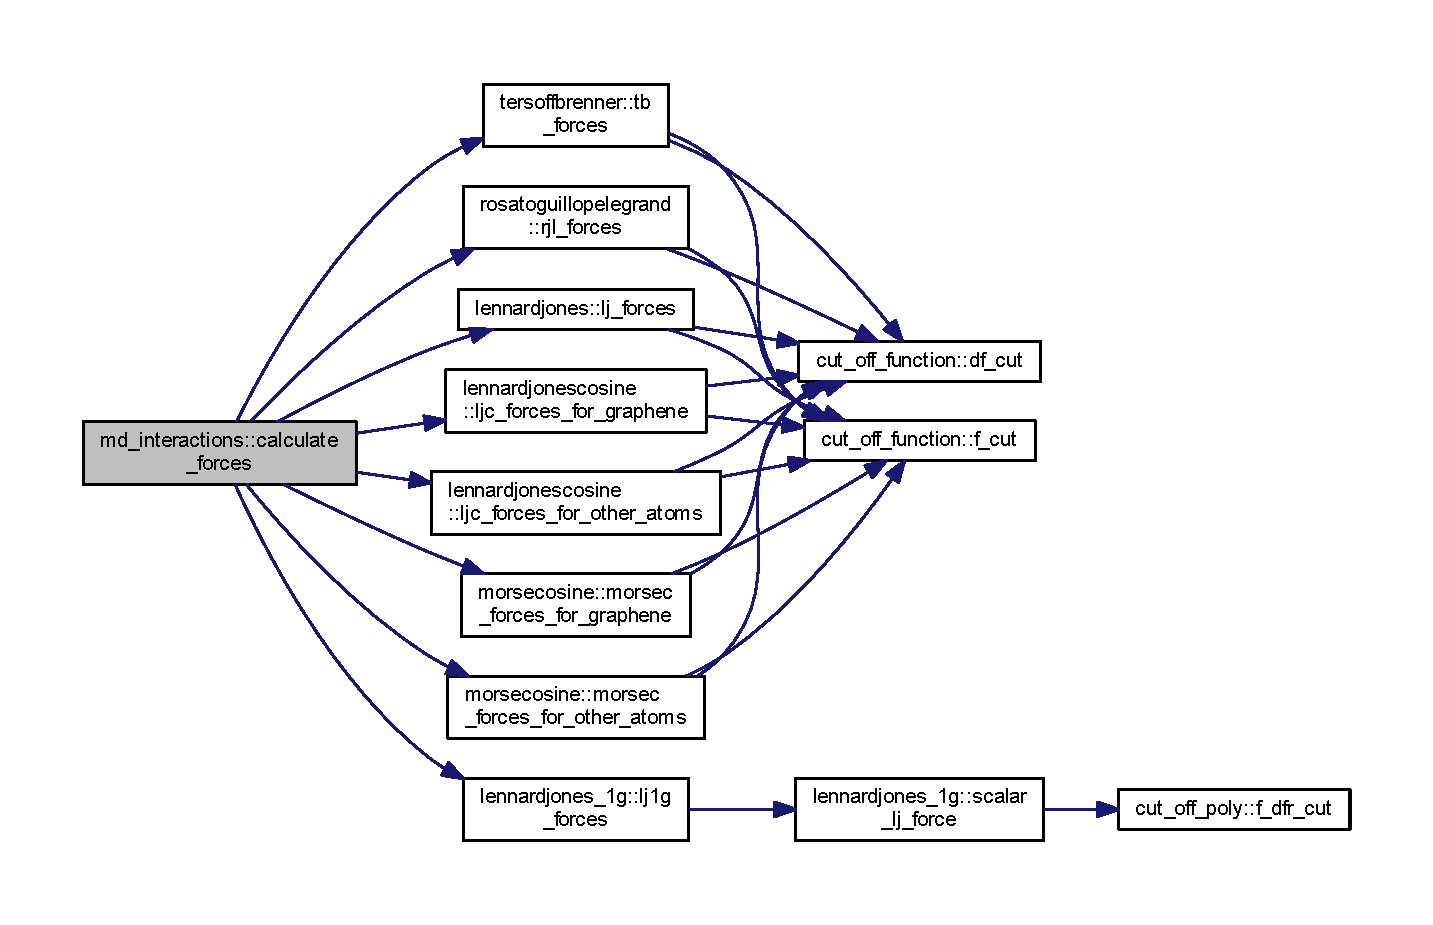
\includegraphics[width=350pt]{namespacemd__interactions_a851acddc07bbaa6d08cf33c60a9e6822_cgraph}
\end{center}
\end{figure}
\mbox{\Hypertarget{namespacemd__interactions_a49c070421fed83b68f06a9b8b7f92048}\label{namespacemd__interactions_a49c070421fed83b68f06a9b8b7f92048}} 
\index{md\+\_\+interactions@{md\+\_\+interactions}!calculate\+\_\+forces\+\_\+numerically@{calculate\+\_\+forces\+\_\+numerically}}
\index{calculate\+\_\+forces\+\_\+numerically@{calculate\+\_\+forces\+\_\+numerically}!md\+\_\+interactions@{md\+\_\+interactions}}
\subsubsection{\texorpdfstring{calculate\+\_\+forces\+\_\+numerically()}{calculate\_forces\_numerically()}}
{\footnotesize\ttfamily subroutine md\+\_\+interactions\+::calculate\+\_\+forces\+\_\+numerically (\begin{DoxyParamCaption}\item[{type(\mbox{\hyperlink{structmd__general_1_1particles}{particles}})}]{atoms,  }\item[{type(\mbox{\hyperlink{structmd__interactions_1_1interaction}{interaction}}), dimension(\+:)}]{interactions }\end{DoxyParamCaption})}



См. определение в файле md\+\_\+interactions.\+f90 строка 274


\begin{DoxyCode}
274     \textcolor{keywordtype}{type}(interaction):: interactions(:)
275     \textcolor{keywordtype}{type}(particles):: atoms
276     \textcolor{keywordtype}{type}(neighbour\_list):: tnl
277     \textcolor{keywordtype}{real}:: e1,e2
278     \textcolor{keywordtype}{integer}:: i,k,inl,j
279     \textcolor{keywordtype}{real},\textcolor{keywordtype}{parameter}:: dx = 10.**(-6)
280 
281     \textcolor{keywordflow}{do} i=1,\textcolor{keyword}{size}(interactions)
282         \textcolor{keywordflow}{if}(interactions(i)%numerical\_force) \textcolor{keywordflow}{then}
283             \textcolor{keywordflow}{select case} (interactions(i)%interaction\_name)
284             \textcolor{keywordflow}{case}(\textcolor{stringliteral}{'ljc'},\textcolor{stringliteral}{'morsec'})\textcolor{comment}{!nl(1) - calc\_tnl(0),add nearest neibls,shift\_nl,shift\_gr\_norm !nl(2) -
       calc\_tnl(0),shift\_nl}
285             \textcolor{keywordflow}{case}(\textcolor{stringliteral}{'lj'},\textcolor{stringliteral}{'morse'},\textcolor{stringliteral}{'tb'},\textcolor{stringliteral}{'rebosc'},\textcolor{stringliteral}{'rjl'})
286                 \textcolor{keywordflow}{do} j=1,interactions(i)%nl\_n
287                     \textcolor{comment}{!$OMP PARALLEL firstprivate(k,inl,e1,e2) private(tnl)}
288                     \textcolor{keyword}{call }create\_truncated\_nl(tnl,interactions(i)%nl(j))
289                     \textcolor{comment}{!$OMP DO}
290                     \textcolor{keywordflow}{do} inl=1,interactions(i)%nl(j)%N
291                         \textcolor{keyword}{call }calculate\_truncated\_nl(tnl,interactions(i)%nl(j),inl,interactions(i)
      %neib\_order)
292                         \textcolor{keywordflow}{do} k=1,3
293                             \textcolor{keyword}{call }shift\_drs(tnl,inl,k,interactions(i)%nl\_n,-dx)
294                             \textcolor{keyword}{call }energy(interactions(i)%interaction\_name,e1,tnl,interactions(i)%parameters)
295                             \textcolor{keyword}{call }shift\_drs(tnl,inl,k,interactions(i)%nl\_n,2*dx)
296                             \textcolor{keyword}{call }energy(interactions(i)%interaction\_name,e2,tnl,interactions(i)%parameters)
297                             \textcolor{keywordflow}{if}(k/=3) \textcolor{keyword}{call }shift\_drs(tnl,inl,k,interactions(i)%nl\_n,-dx)
298                             atoms%forces(k,interactions(i)%nl(j)%particle\_index(inl)) =&
299                             atoms%forces(k,interactions(i)%nl(j)%particle\_index(inl))+(e1-e2)/2/dx
300 \textcolor{keywordflow}{                        enddo}
301 \textcolor{keywordflow}{                    enddo}
302                     \textcolor{comment}{!$OMP END DO}
303                     \textcolor{keyword}{call }destroy\_truncated\_nl(tnl)
304                     \textcolor{comment}{!$OMP END PARALLEL}
305 \textcolor{keywordflow}{                enddo}
306 \textcolor{keywordflow}{            end select}
307 \textcolor{keywordflow}{        endif}
308 \textcolor{keywordflow}{    enddo}
309     
\end{DoxyCode}
Граф вызовов\+:\nopagebreak
\begin{figure}[H]
\begin{center}
\leavevmode
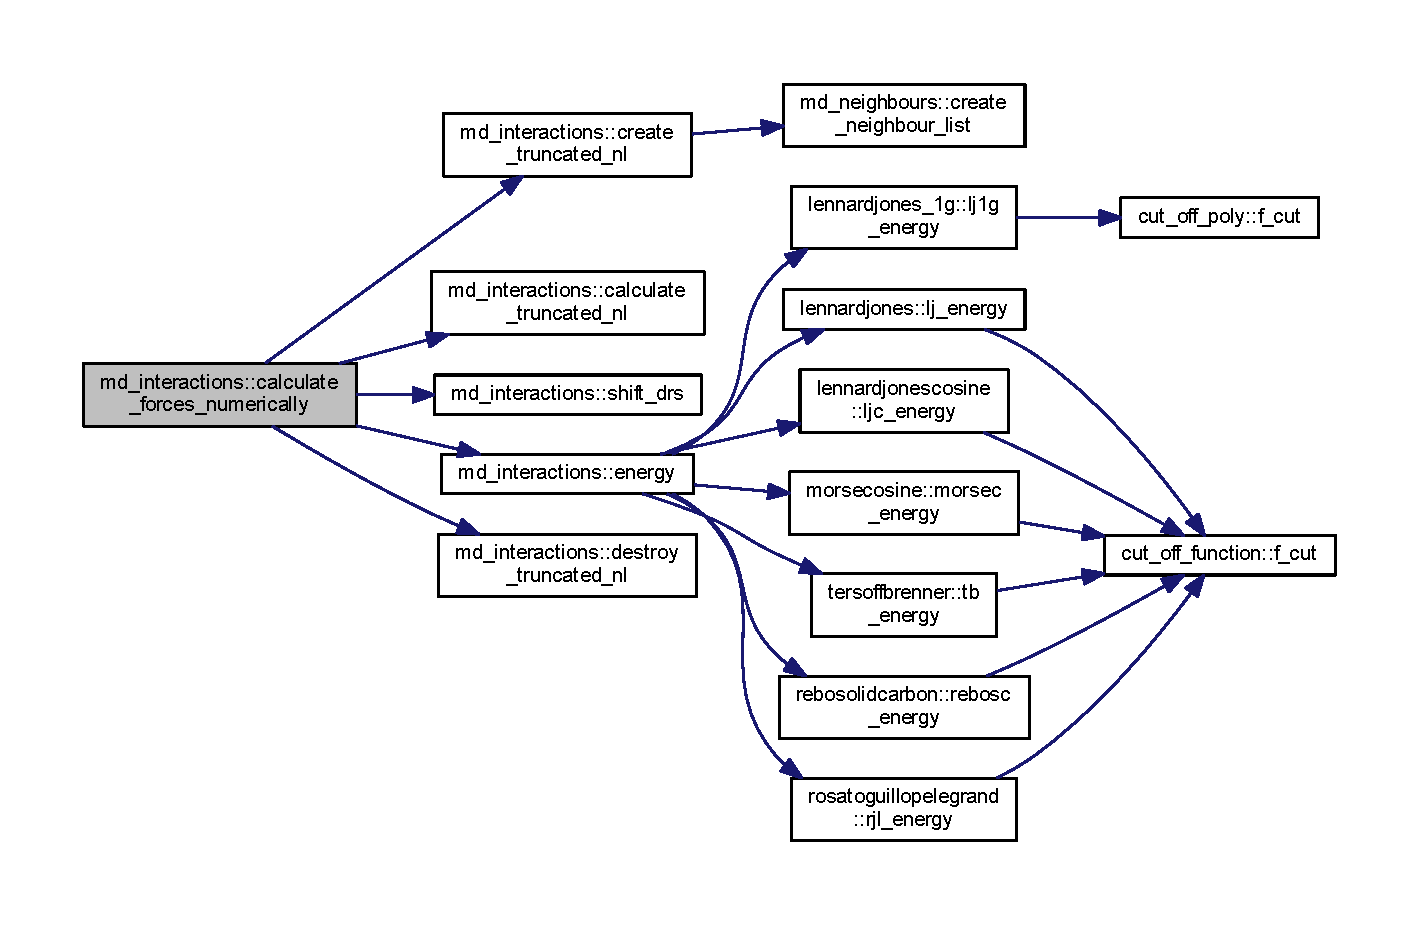
\includegraphics[width=350pt]{namespacemd__interactions_a49c070421fed83b68f06a9b8b7f92048_cgraph}
\end{center}
\end{figure}
\mbox{\Hypertarget{namespacemd__interactions_a846dbc2db901133c72ff58afb321e918}\label{namespacemd__interactions_a846dbc2db901133c72ff58afb321e918}} 
\index{md\+\_\+interactions@{md\+\_\+interactions}!calculate\+\_\+potential\+\_\+energies@{calculate\+\_\+potential\+\_\+energies}}
\index{calculate\+\_\+potential\+\_\+energies@{calculate\+\_\+potential\+\_\+energies}!md\+\_\+interactions@{md\+\_\+interactions}}
\subsubsection{\texorpdfstring{calculate\+\_\+potential\+\_\+energies()}{calculate\_potential\_energies()}}
{\footnotesize\ttfamily subroutine md\+\_\+interactions\+::calculate\+\_\+potential\+\_\+energies (\begin{DoxyParamCaption}\item[{type(\mbox{\hyperlink{structmd__interactions_1_1interaction}{interaction}}), dimension(\+:)}]{interactions }\end{DoxyParamCaption})}



См. определение в файле md\+\_\+interactions.\+f90 строка 264


\begin{DoxyCode}
264     \textcolor{keywordtype}{type}(interaction):: interactions(:)
265     \textcolor{keywordtype}{integer}:: i
266     
267     \textcolor{keywordflow}{do} i=1,\textcolor{keyword}{size}(interactions)
268         \textcolor{keyword}{call }energy(interactions(i)%interaction\_name,interactions(i)%energy,interactions(i)%nl(1),
      interactions(i)%parameters)
269 \textcolor{keywordflow}{    enddo}
270         
\end{DoxyCode}
Граф вызовов\+:\nopagebreak
\begin{figure}[H]
\begin{center}
\leavevmode
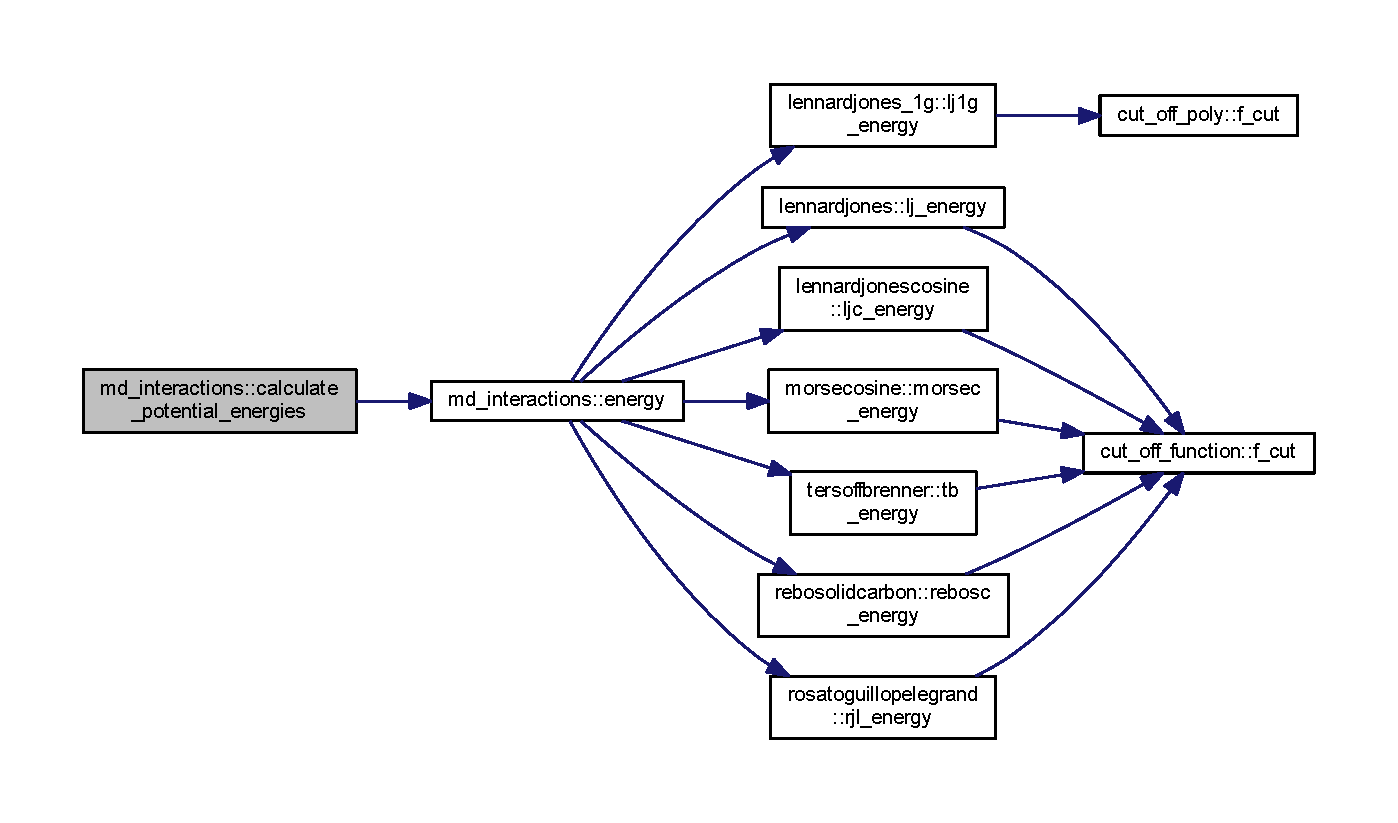
\includegraphics[width=350pt]{namespacemd__interactions_a846dbc2db901133c72ff58afb321e918_cgraph}
\end{center}
\end{figure}
\mbox{\Hypertarget{namespacemd__interactions_abc7ac3a3b1e9382804836d43cdc9a224}\label{namespacemd__interactions_abc7ac3a3b1e9382804836d43cdc9a224}} 
\index{md\+\_\+interactions@{md\+\_\+interactions}!calculate\+\_\+truncated\+\_\+nl@{calculate\+\_\+truncated\+\_\+nl}}
\index{calculate\+\_\+truncated\+\_\+nl@{calculate\+\_\+truncated\+\_\+nl}!md\+\_\+interactions@{md\+\_\+interactions}}
\subsubsection{\texorpdfstring{calculate\+\_\+truncated\+\_\+nl()}{calculate\_truncated\_nl()}}
{\footnotesize\ttfamily subroutine md\+\_\+interactions\+::calculate\+\_\+truncated\+\_\+nl (\begin{DoxyParamCaption}\item[{type(\mbox{\hyperlink{structmd__general_1_1neighbour__list}{neighbour\+\_\+list}})}]{tnl,  }\item[{type(\mbox{\hyperlink{structmd__general_1_1neighbour__list}{neighbour\+\_\+list}})}]{nl,  }\item[{integer}]{i,  }\item[{integer}]{n }\end{DoxyParamCaption})}



См. определение в файле md\+\_\+interactions.\+f90 строка 335


\begin{DoxyCode}
335     \textcolor{keywordtype}{type}(neighbour\_list):: tnl,nl
336     \textcolor{keywordtype}{integer}:: n,i,ni,p,q,j
337     
338     tnl%particle\_index = 0; tnl%nnum = 0; \textcolor{comment}{!tnl%nlist = 0!tnl%dr = 0.!tnl%moddr = 0.}
339     
340     tnl%N = nl%N
341     tnl%neighb\_num\_max = nl%neighb\_num\_max
342     tnl%nlist(:nl%nnum(i),i) = nl%nlist(:nl%nnum(i),i)
343     tnl%dr(:,:nl%nnum(i),i) = nl%dr(:,:nl%nnum(i),i)
344     tnl%moddr(:nl%nnum(i),i) = nl%moddr(:nl%nnum(i),i)
345     tnl%nnum(i) = nl%nnum(i)
346     tnl%particle\_index(i) = nl%particle\_index(i)
347     \textcolor{keywordflow}{do} ni=1,n
348         \textcolor{keywordflow}{if}(ni<n) \textcolor{keywordflow}{then}
349             \textcolor{keywordflow}{do} j=1,tnl%N
350                 \textcolor{keywordflow}{do} p=1,tnl%nnum(j)
351                     q = tnl%nlist(p,j)
352                     \textcolor{keywordflow}{if}(tnl%nnum(q)==0) \textcolor{keywordflow}{then}
353                         tnl%nlist(:nl%nnum(q),q) = nl%nlist(:nl%nnum(q),q)
354                         tnl%dr(:,:nl%nnum(q),q) = nl%dr(:,:nl%nnum(q),q)
355                         tnl%moddr(:nl%nnum(q),q) = nl%moddr(:nl%nnum(q),q)
356                         tnl%particle\_index(q) = nl%particle\_index(q)
357 \textcolor{keywordflow}{                    endif}
358 \textcolor{keywordflow}{                enddo}
359 \textcolor{keywordflow}{            enddo}
360             \textcolor{keywordflow}{do} j=1,tnl%N
361                 \textcolor{keywordflow}{if}(tnl%particle\_index(j)/=0) tnl%nnum(j) = nl%nnum(j)
362 \textcolor{keywordflow}{            enddo}
363         \textcolor{keywordflow}{else}
364             \textcolor{keywordflow}{do} j=1,tnl%N
365                 \textcolor{keywordflow}{do} p=1,tnl%nnum(j)
366                     q = tnl%nlist(p,j)
367                     \textcolor{keywordflow}{if}(tnl%nnum(q)==0) \textcolor{keywordflow}{then}
368                         tnl%nnum(q) = tnl%nnum(q)+1
369                         tnl%nlist(tnl%nnum(q),q) = j
370                         tnl%dr(:,tnl%nnum(q),q) = -nl%dr(:,p,j)
371                         tnl%moddr(tnl%nnum(q),q) = nl%moddr(p,j)
372                         tnl%particle\_index(q) = nl%particle\_index(q)
373 \textcolor{keywordflow}{                    endif}
374 \textcolor{keywordflow}{                enddo}
375 \textcolor{keywordflow}{            enddo}
376 \textcolor{keywordflow}{        endif}
377 \textcolor{keywordflow}{    enddo}
378     
\end{DoxyCode}
\mbox{\Hypertarget{namespacemd__interactions_a52c7d3a0c8df2f15b75c8fef73ee795d}\label{namespacemd__interactions_a52c7d3a0c8df2f15b75c8fef73ee795d}} 
\index{md\+\_\+interactions@{md\+\_\+interactions}!create\+\_\+groups@{create\+\_\+groups}}
\index{create\+\_\+groups@{create\+\_\+groups}!md\+\_\+interactions@{md\+\_\+interactions}}
\subsubsection{\texorpdfstring{create\+\_\+groups()}{create\_groups()}}
{\footnotesize\ttfamily subroutine md\+\_\+interactions\+::create\+\_\+groups (\begin{DoxyParamCaption}\item[{type(\mbox{\hyperlink{structmd__general_1_1particle__group}{particle\+\_\+group}}), dimension(\+:), allocatable}]{groups,  }\item[{integer}]{file\+\_\+id,  }\item[{integer}]{out\+\_\+id,  }\item[{type(\mbox{\hyperlink{structmd__general_1_1particles}{particles}})}]{atoms }\end{DoxyParamCaption})}



См. определение в файле md\+\_\+interactions.\+f90 строка 39


\begin{DoxyCode}
39     \textcolor{keywordtype}{type}(particle\_group),\textcolor{keywordtype}{allocatable}:: groups(:)
40     \textcolor{keywordtype}{type}(particles):: atoms
41     \textcolor{keywordtype}{character(len=32)},\textcolor{keywordtype}{allocatable}:: type\_names(:,:)
42     \textcolor{keywordtype}{character(len=128)}:: str,frmt
43     \textcolor{keywordtype}{integer}:: i,particle\_types\_num,groups\_num,file\_id,out\_id
44     
45     \textcolor{keyword}{read}(file\_id,*) str,particle\_types\_num
46     \textcolor{keyword}{write}(out\_id,\textcolor{stringliteral}{'(A32,i12)'}) str,particle\_types\_num
47     \textcolor{keyword}{read}(file\_id,*) str,groups\_num
48     \textcolor{keyword}{write}(out\_id,\textcolor{stringliteral}{'(A32,i12)'}) str,groups\_num
49     \textcolor{keyword}{allocate}(groups(groups\_num),type\_names(particle\_types\_num,groups\_num))
50     \textcolor{keyword}{write}(frmt,\textcolor{stringliteral}{'("(i6,A,",i0,"A12,i9)")'}) particle\_types\_num
51     \textcolor{keywordflow}{do} i=1,groups\_num
52         \textcolor{keyword}{read}(file\_id,*) str,type\_names(:,i)
53         \textcolor{keyword}{call }create\_particle\_group(groups(i),type\_names(:,i),atoms)
54         \textcolor{keyword}{write}(out\_id,frmt) i,\textcolor{stringliteral}{' '},type\_names(:,i),groups(i)%N
55 \textcolor{keywordflow}{    enddo}
56     
\end{DoxyCode}
Граф вызовов\+:\nopagebreak
\begin{figure}[H]
\begin{center}
\leavevmode
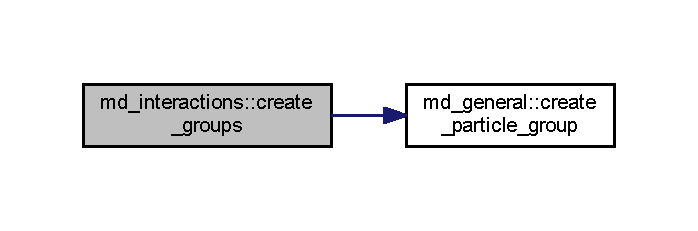
\includegraphics[width=335pt]{namespacemd__interactions_a52c7d3a0c8df2f15b75c8fef73ee795d_cgraph}
\end{center}
\end{figure}
\mbox{\Hypertarget{namespacemd__interactions_ad655aab8b55d15d13e66769ae95ca229}\label{namespacemd__interactions_ad655aab8b55d15d13e66769ae95ca229}} 
\index{md\+\_\+interactions@{md\+\_\+interactions}!create\+\_\+interactions@{create\+\_\+interactions}}
\index{create\+\_\+interactions@{create\+\_\+interactions}!md\+\_\+interactions@{md\+\_\+interactions}}
\subsubsection{\texorpdfstring{create\+\_\+interactions()}{create\_interactions()}}
{\footnotesize\ttfamily subroutine md\+\_\+interactions\+::create\+\_\+interactions (\begin{DoxyParamCaption}\item[{type(\mbox{\hyperlink{structmd__interactions_1_1interaction}{interaction}}), dimension(\+:), allocatable}]{interactions,  }\item[{type(\mbox{\hyperlink{structmd__general_1_1particle__group}{particle\+\_\+group}}), dimension(\+:)}]{groups,  }\item[{integer}]{file\+\_\+id,  }\item[{integer}]{out\+\_\+id,  }\item[{character(len=128)}]{input\+\_\+path }\end{DoxyParamCaption})}



См. определение в файле md\+\_\+interactions.\+f90 строка 60


\begin{DoxyCode}
60     \textcolor{keywordtype}{type}(interaction),\textcolor{keywordtype}{allocatable}:: interactions(:)
61     \textcolor{keywordtype}{type}(particle\_group):: groups(:)
62     \textcolor{keywordtype}{integer}:: file\_id,out\_id,i,j,inter\_n
63     \textcolor{keywordtype}{character(len=128)}:: input\_path,str
64     
65     \textcolor{keyword}{read}(file\_id,*) str,inter\_n
66     \textcolor{keyword}{write}(out\_id,\textcolor{stringliteral}{'(A32,i12)'}) str,inter\_n
67     \textcolor{keyword}{allocate}(interactions(inter\_n))
68     \textcolor{keywordflow}{do} i=1,inter\_n
69         \textcolor{keyword}{read}(file\_id,*) interactions(i)%interaction\_name,interactions(i)%parameters\_file
70         \textcolor{keywordflow}{select case} (interactions(i)%interaction\_name)
71         \textcolor{keywordflow}{case}(\textcolor{stringliteral}{'lj'})
72             \textcolor{keyword}{allocate}(interactions(i)%parameters%LJ(1))
73             \textcolor{keyword}{call }read\_lj\_parameters(interactions(i)%parameters%LJ(1),trim(input\_path)//interactions(i)
      %parameters\_file)
74             interactions(i)%nl\_n = 2
75             interactions(i)%neib\_order = 0
76             interactions(i)%numerical\_force = .false.
77         \textcolor{keywordflow}{case}(\textcolor{stringliteral}{'lj1g'})
78             \textcolor{keyword}{allocate}(interactions(i)%parameters%LJ1g(1))
79             \textcolor{keyword}{call }read\_lj1g\_parameters(interactions(i)%parameters%LJ1g(1),trim(input\_path)//interactions(i)
      %parameters\_file)
80             interactions(i)%nl\_n = 1
81             interactions(i)%neib\_order = 0
82             interactions(i)%numerical\_force = .false.
83         \textcolor{comment}{!case('morse')}
84         \textcolor{comment}{!   allocate(interactions(i)%parameters%Morse(1))}
85         \textcolor{comment}{!   call
       read\_Morse\_parameters(interactions(i)%parameters%Morse(1),trim(input\_path)//interactions(i)%parameters\_file)}
86         \textcolor{comment}{!   interactions(i)%nl\_n = 2}
87         \textcolor{comment}{!   interactions(i)%neib\_order = 0}
88         \textcolor{comment}{!   interactions(i)%numerical\_force = .false.}
89         \textcolor{keywordflow}{case}(\textcolor{stringliteral}{'ljc'})
90             \textcolor{keyword}{allocate}(interactions(i)%parameters%LJC(1))
91             \textcolor{keyword}{call }read\_ljc\_parameters(interactions(i)%parameters%LJC(1),trim(input\_path)//interactions(i)
      %parameters\_file)
92             interactions(i)%nl\_n = 3
93             interactions(i)%neib\_order = 0
94             interactions(i)%numerical\_force = .false.
95         \textcolor{keywordflow}{case}(\textcolor{stringliteral}{'morsec'})
96             \textcolor{keyword}{allocate}(interactions(i)%parameters%MorseC(1))
97             \textcolor{keyword}{call }read\_morsec\_parameters(interactions(i)%parameters%MorseC(1),trim(input\_path)//interactions
      (i)%parameters\_file)
98             interactions(i)%nl\_n = 3
99             interactions(i)%neib\_order = 0
100             interactions(i)%numerical\_force = .false.
101         \textcolor{keywordflow}{case}(\textcolor{stringliteral}{'tb'})
102             \textcolor{keyword}{allocate}(interactions(i)%parameters%TB(1))
103             \textcolor{keyword}{call }read\_tb\_parameters(interactions(i)%parameters%TB(1),trim(input\_path)//interactions(i)
      %parameters\_file)
104             interactions(i)%nl\_n = 1
105             interactions(i)%neib\_order = 2
106             interactions(i)%numerical\_force = .false.
107         \textcolor{keywordflow}{case}(\textcolor{stringliteral}{'rebosc'})
108             \textcolor{keyword}{allocate}(interactions(i)%parameters%REBOsc(1))
109             \textcolor{keyword}{call }read\_rebosc\_parameters(interactions(i)%parameters%REBOsc(1),trim(input\_path)//interactions
      (i)%parameters\_file)
110             interactions(i)%nl\_n = 1
111             interactions(i)%neib\_order = 3
112             interactions(i)%numerical\_force = .true.            
113         \textcolor{keywordflow}{case}(\textcolor{stringliteral}{'rjl'})
114             \textcolor{keyword}{allocate}(interactions(i)%parameters%RJL(1))
115             \textcolor{keyword}{call }read\_rjl\_parameters(interactions(i)%parameters%RJL(1),trim(input\_path)//interactions(i)
      %parameters\_file)
116             interactions(i)%nl\_n = 1
117             interactions(i)%neib\_order = 2
118             interactions(i)%numerical\_force = .false.
119 \textcolor{keywordflow}{        case default}
120             print*,\textcolor{stringliteral}{'error: unknown interaction name'}
121 \textcolor{keywordflow}{        end select}
122         \textcolor{keyword}{write}(out\_id,\textcolor{stringliteral}{'(2A32,i6)'}) interactions(i)%interaction\_name,interactions(i)%parameters\_file,
      interactions(i)%nl\_n
123         \textcolor{keyword}{allocate}(interactions(i)%group\_nums(2*interactions(i)%nl\_n))
124         \textcolor{keyword}{allocate}(interactions(i)%nl(interactions(i)%nl\_n))
125         \textcolor{keywordflow}{do} j=1,interactions(i)%nl\_n
126             \textcolor{keyword}{read}(file\_id,*) interactions(i)%group\_nums(j*2-1:j*2),&
127             interactions(i)%nl(j)%neighb\_num\_max,interactions(i)%nl(j)%r\_cut,interactions(i)%nl(j)
      %update\_period
128             \textcolor{keyword}{write}(out\_id,\textcolor{stringliteral}{'(3i6,f16.6,i9)'}) interactions(i)%group\_nums(j*2-1:j*2),&
129             interactions(i)%nl(j)%neighb\_num\_max,interactions(i)%nl(j)%r\_cut,interactions(i)%nl(j)
      %update\_period
130             interactions(i)%nl(j)%N = groups(interactions(i)%group\_nums(j*2-1))%N
131             \textcolor{keyword}{call }create\_neighbour\_list(interactions(i)%nl(j))
132 \textcolor{keywordflow}{        enddo}
133 \textcolor{keywordflow}{    enddo}
134     \textcolor{keyword}{call }allocate\_graphene\_norm(interactions)
135     
\end{DoxyCode}
Граф вызовов\+:\nopagebreak
\begin{figure}[H]
\begin{center}
\leavevmode
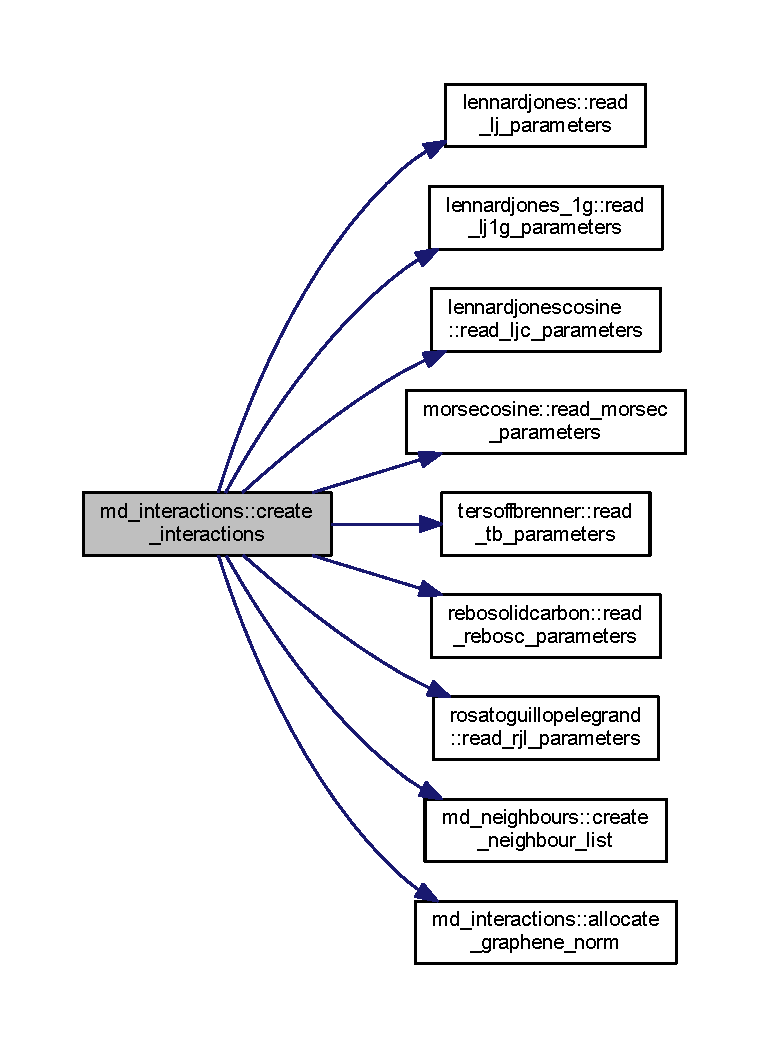
\includegraphics[width=350pt]{namespacemd__interactions_ad655aab8b55d15d13e66769ae95ca229_cgraph}
\end{center}
\end{figure}
\mbox{\Hypertarget{namespacemd__interactions_aac3f945d504b95d25098bb5d5d5f4208}\label{namespacemd__interactions_aac3f945d504b95d25098bb5d5d5f4208}} 
\index{md\+\_\+interactions@{md\+\_\+interactions}!create\+\_\+truncated\+\_\+nl@{create\+\_\+truncated\+\_\+nl}}
\index{create\+\_\+truncated\+\_\+nl@{create\+\_\+truncated\+\_\+nl}!md\+\_\+interactions@{md\+\_\+interactions}}
\subsubsection{\texorpdfstring{create\+\_\+truncated\+\_\+nl()}{create\_truncated\_nl()}}
{\footnotesize\ttfamily subroutine md\+\_\+interactions\+::create\+\_\+truncated\+\_\+nl (\begin{DoxyParamCaption}\item[{type(\mbox{\hyperlink{structmd__general_1_1neighbour__list}{neighbour\+\_\+list}})}]{tnl,  }\item[{type(\mbox{\hyperlink{structmd__general_1_1neighbour__list}{neighbour\+\_\+list}})}]{nl }\end{DoxyParamCaption})}



См. определение в файле md\+\_\+interactions.\+f90 строка 313


\begin{DoxyCode}
313     \textcolor{keywordtype}{type}(neighbour\_list):: tnl,nl
314     
315     tnl%N = nl%N
316     tnl%neighb\_num\_max = nl%neighb\_num\_max
317     \textcolor{keyword}{call }create\_neighbour\_list(tnl)
318     
\end{DoxyCode}
Граф вызовов\+:\nopagebreak
\begin{figure}[H]
\begin{center}
\leavevmode
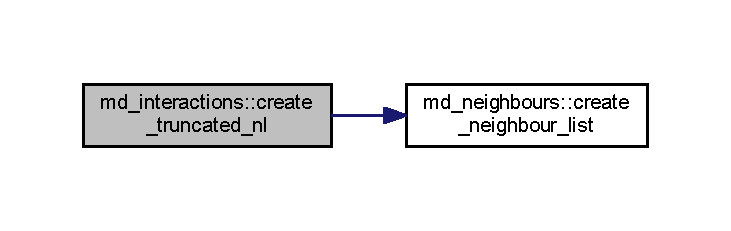
\includegraphics[width=350pt]{namespacemd__interactions_aac3f945d504b95d25098bb5d5d5f4208_cgraph}
\end{center}
\end{figure}
\mbox{\Hypertarget{namespacemd__interactions_a36f14223ced172ec4c9a9bc381384b55}\label{namespacemd__interactions_a36f14223ced172ec4c9a9bc381384b55}} 
\index{md\+\_\+interactions@{md\+\_\+interactions}!destroy\+\_\+truncated\+\_\+nl@{destroy\+\_\+truncated\+\_\+nl}}
\index{destroy\+\_\+truncated\+\_\+nl@{destroy\+\_\+truncated\+\_\+nl}!md\+\_\+interactions@{md\+\_\+interactions}}
\subsubsection{\texorpdfstring{destroy\+\_\+truncated\+\_\+nl()}{destroy\_truncated\_nl()}}
{\footnotesize\ttfamily subroutine md\+\_\+interactions\+::destroy\+\_\+truncated\+\_\+nl (\begin{DoxyParamCaption}\item[{type(\mbox{\hyperlink{structmd__general_1_1neighbour__list}{neighbour\+\_\+list}})}]{tnl }\end{DoxyParamCaption})}



См. определение в файле md\+\_\+interactions.\+f90 строка 322


\begin{DoxyCode}
322     \textcolor{keywordtype}{type}(neighbour\_list):: tnl
323     
324     tnl%N = 0
325     tnl%neighb\_num\_max = 0
326     \textcolor{keywordflow}{if}(\textcolor{keyword}{allocated}(tnl%particle\_index)) \textcolor{keyword}{deallocate}(tnl%particle\_index)
327     \textcolor{keywordflow}{if}(\textcolor{keyword}{allocated}(tnl%nnum)) \textcolor{keyword}{deallocate}(tnl%nnum)
328     \textcolor{keywordflow}{if}(\textcolor{keyword}{allocated}(tnl%nlist)) \textcolor{keyword}{deallocate}(tnl%nlist)
329     \textcolor{keywordflow}{if}(\textcolor{keyword}{allocated}(tnl%dr)) \textcolor{keyword}{deallocate}(tnl%dr)
330     \textcolor{keywordflow}{if}(\textcolor{keyword}{allocated}(tnl%moddr)) \textcolor{keyword}{deallocate}(tnl%moddr)
331     
\end{DoxyCode}
\mbox{\Hypertarget{namespacemd__interactions_a5b3213ff25495c56eeabce8427fb3082}\label{namespacemd__interactions_a5b3213ff25495c56eeabce8427fb3082}} 
\index{md\+\_\+interactions@{md\+\_\+interactions}!energy@{energy}}
\index{energy@{energy}!md\+\_\+interactions@{md\+\_\+interactions}}
\subsubsection{\texorpdfstring{energy()}{energy()}}
{\footnotesize\ttfamily subroutine md\+\_\+interactions\+::energy (\begin{DoxyParamCaption}\item[{character(len=32)}]{inter\+\_\+name,  }\item[{real}]{e,  }\item[{type(\mbox{\hyperlink{structmd__general_1_1neighbour__list}{neighbour\+\_\+list}})}]{nl,  }\item[{type(\mbox{\hyperlink{structmd__interactions_1_1interaction__parameters}{interaction\+\_\+parameters}})}]{p }\end{DoxyParamCaption})}



См. определение в файле md\+\_\+interactions.\+f90 строка 245


\begin{DoxyCode}
245     \textcolor{keywordtype}{type}(interaction\_parameters):: p
246     \textcolor{keywordtype}{type}(neighbour\_list):: nl
247     \textcolor{keywordtype}{character(len=32)}:: inter\_name
248     \textcolor{keywordtype}{real}:: e
249     
250     \textcolor{keywordflow}{select case} (inter\_name)
251     \textcolor{keywordflow}{case}(\textcolor{stringliteral}{'lj'});     \textcolor{keyword}{call }lj\_energy(e,nl,p%LJ(1))
252     \textcolor{keywordflow}{case}(\textcolor{stringliteral}{'lj1g'});   \textcolor{keyword}{call }lj1g\_energy(e,nl,p%LJ1g(1))
253     \textcolor{comment}{!case('morse');}
254     \textcolor{keywordflow}{case}(\textcolor{stringliteral}{'ljc'});    \textcolor{keyword}{call }ljc\_energy(e,nl,p%LJC(1))
255     \textcolor{keywordflow}{case}(\textcolor{stringliteral}{'morsec'}); \textcolor{keyword}{call }morsec\_energy(e,nl,p%MorseC(1))
256     \textcolor{keywordflow}{case}(\textcolor{stringliteral}{'tb'});     \textcolor{keyword}{call }tb\_energy(e,nl,p%TB(1))
257     \textcolor{keywordflow}{case}(\textcolor{stringliteral}{'rebosc'}); \textcolor{keyword}{call }rebosc\_energy(e,nl,p%REBOsc(1))
258     \textcolor{keywordflow}{case}(\textcolor{stringliteral}{'rjl'});    \textcolor{keyword}{call }rjl\_energy(e,nl,p%RJL(1))
259 \textcolor{keywordflow}{    end select}
260     
\end{DoxyCode}
Граф вызовов\+:\nopagebreak
\begin{figure}[H]
\begin{center}
\leavevmode
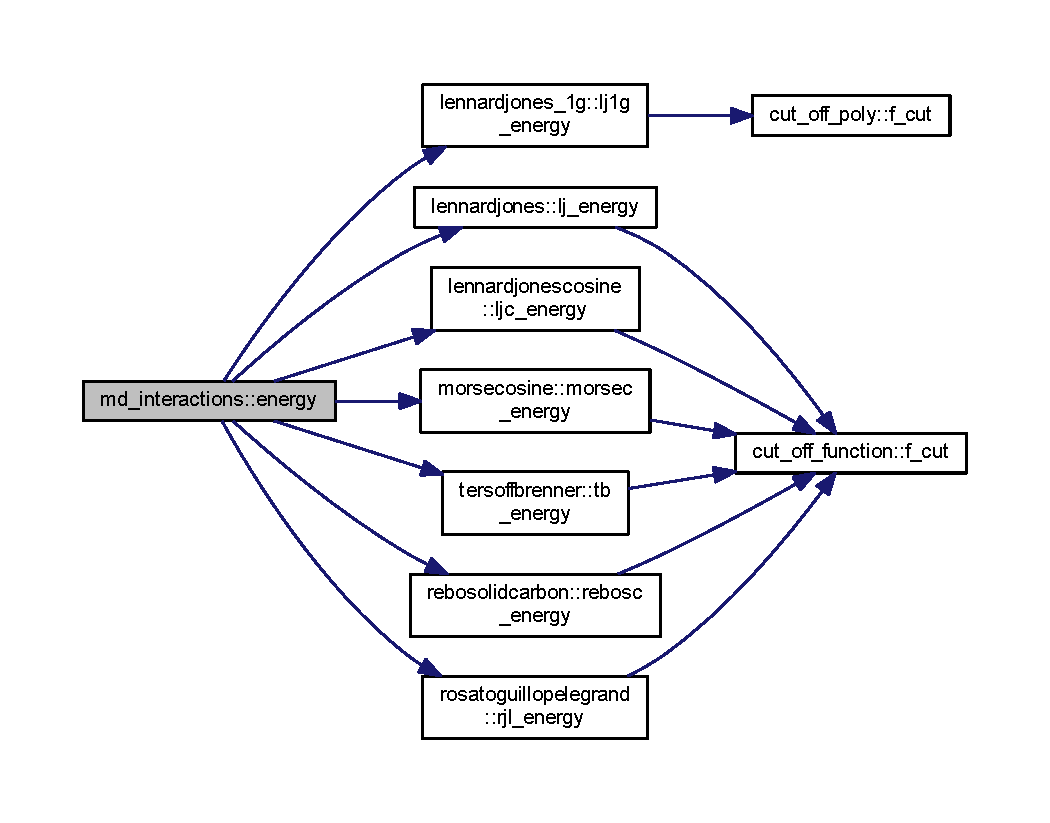
\includegraphics[width=350pt]{namespacemd__interactions_a5b3213ff25495c56eeabce8427fb3082_cgraph}
\end{center}
\end{figure}
\mbox{\Hypertarget{namespacemd__interactions_a5787116d9c766f3d3ec6355c299d58c2}\label{namespacemd__interactions_a5787116d9c766f3d3ec6355c299d58c2}} 
\index{md\+\_\+interactions@{md\+\_\+interactions}!nlists\+\_\+load@{nlists\+\_\+load}}
\index{nlists\+\_\+load@{nlists\+\_\+load}!md\+\_\+interactions@{md\+\_\+interactions}}
\subsubsection{\texorpdfstring{nlists\+\_\+load()}{nlists\_load()}}
{\footnotesize\ttfamily subroutine md\+\_\+interactions\+::nlists\+\_\+load (\begin{DoxyParamCaption}\item[{integer}]{out\+\_\+id,  }\item[{type(\mbox{\hyperlink{structmd__interactions_1_1interaction}{interaction}}), dimension(\+:)}]{interactions }\end{DoxyParamCaption})}



См. определение в файле md\+\_\+interactions.\+f90 строка 428


\begin{DoxyCode}
428     \textcolor{keywordtype}{type}(interaction):: interactions(:)
429     \textcolor{keywordtype}{integer}:: i,j,out\_id
430     
431     \textcolor{keywordflow}{if}(\textcolor{keyword}{size}(interactions)>0) \textcolor{keyword}{write}(out\_id,\textcolor{stringliteral}{'(A)'}) \textcolor{stringliteral}{' neib lists load:'}     
432     \textcolor{keywordflow}{do} i=1,\textcolor{keyword}{size}(interactions)
433         \textcolor{keywordflow}{do} j=1,interactions(i)%nl\_n
434             \textcolor{keywordflow}{if}(interactions(i)%nl(j)%N>0) \textcolor{keywordflow}{then}
435                 \textcolor{keyword}{write}(out\_id,\textcolor{stringliteral}{'(A12,i6,i6,A,i6)'}) trim(interactions(i)%interaction\_name),j,&
436                 maxval(interactions(i)%nl(j)%nnum),\textcolor{stringliteral}{'/'},interactions(i)%nl(j)%neighb\_num\_max
437             \textcolor{keywordflow}{else}
438                 \textcolor{keyword}{write}(out\_id,\textcolor{stringliteral}{'(A12,i6,i6,A,i6)'}) trim(interactions(i)%interaction\_name),j,&
439                 0,\textcolor{stringliteral}{'/'},interactions(i)%nl(j)%neighb\_num\_max
440 \textcolor{keywordflow}{            endif}
441 \textcolor{keywordflow}{        enddo}
442 \textcolor{keywordflow}{    enddo}
443     
\end{DoxyCode}
\mbox{\Hypertarget{namespacemd__interactions_a4cbfd0c1d189320866efb63454722170}\label{namespacemd__interactions_a4cbfd0c1d189320866efb63454722170}} 
\index{md\+\_\+interactions@{md\+\_\+interactions}!shift\+\_\+drs@{shift\+\_\+drs}}
\index{shift\+\_\+drs@{shift\+\_\+drs}!md\+\_\+interactions@{md\+\_\+interactions}}
\subsubsection{\texorpdfstring{shift\+\_\+drs()}{shift\_drs()}}
{\footnotesize\ttfamily subroutine md\+\_\+interactions\+::shift\+\_\+drs (\begin{DoxyParamCaption}\item[{type(\mbox{\hyperlink{structmd__general_1_1neighbour__list}{neighbour\+\_\+list}})}]{tnl,  }\item[{integer}]{inl,  }\item[{integer}]{k,  }\item[{integer}]{nl\+\_\+n,  }\item[{real}]{dx }\end{DoxyParamCaption})}



См. определение в файле md\+\_\+interactions.\+f90 строка 382


\begin{DoxyCode}
382     \textcolor{keywordtype}{type}(neighbour\_list):: tnl
383     \textcolor{keywordtype}{real}:: dx
384     \textcolor{keywordtype}{integer}:: p,k,inl,q,j,nl\_n
385     
386     \textcolor{keywordflow}{do} p=1,tnl%nnum(inl)
387         tnl%dr(k,p,inl) = tnl%dr(k,p,inl)-dx
388         tnl%moddr(p,inl) = sqrt(sum(tnl%dr(:,p,inl)**2))
389 \textcolor{keywordflow}{    enddo}
390     \textcolor{keywordflow}{if}(nl\_n==1) \textcolor{keywordflow}{then}
391         \textcolor{keywordflow}{do} j=1,tnl%N
392             \textcolor{keywordflow}{do} p=1,tnl%nnum(j)
393                 q = tnl%nlist(p,j)
394                 \textcolor{keywordflow}{if}(q==inl) \textcolor{keywordflow}{then}
395                     tnl%dr(k,p,j) = tnl%dr(k,p,j)+dx
396                     tnl%moddr(p,j) = sqrt(sum(tnl%dr(:,p,j)**2))
397 \textcolor{keywordflow}{                endif}
398 \textcolor{keywordflow}{            enddo}
399 \textcolor{keywordflow}{        enddo}
400 \textcolor{keywordflow}{    endif}
401 
\end{DoxyCode}
\mbox{\Hypertarget{namespacemd__interactions_a2c4725fefbad36399f5de45a222b5d4e}\label{namespacemd__interactions_a2c4725fefbad36399f5de45a222b5d4e}} 
\index{md\+\_\+interactions@{md\+\_\+interactions}!shift\+\_\+gr\+\_\+norm@{shift\+\_\+gr\+\_\+norm}}
\index{shift\+\_\+gr\+\_\+norm@{shift\+\_\+gr\+\_\+norm}!md\+\_\+interactions@{md\+\_\+interactions}}
\subsubsection{\texorpdfstring{shift\+\_\+gr\+\_\+norm()}{shift\_gr\_norm()}}
{\footnotesize\ttfamily subroutine md\+\_\+interactions\+::shift\+\_\+gr\+\_\+norm (\begin{DoxyParamCaption}\item[{real, dimension(\+:,\+:)}]{gr\+\_\+norm,  }\item[{type(\mbox{\hyperlink{structmd__general_1_1neighbour__list}{neighbour\+\_\+list}})}]{nl\+\_\+nn,  }\item[{integer}]{inl,  }\item[{integer}]{k,  }\item[{real}]{dx }\end{DoxyParamCaption})}



См. определение в файле md\+\_\+interactions.\+f90 строка 405


\begin{DoxyCode}
405     \textcolor{keywordtype}{real}:: gr\_norm(:,:)
406     \textcolor{keywordtype}{type}(neighbour\_list):: nl\_nn
407     \textcolor{keywordtype}{real}:: dx,drj12(3),drj31(3)
408     \textcolor{keywordtype}{integer}:: k,inl,p,q,j,l
409     
410     \textcolor{keywordflow}{do} p=1,nl\_nn%nnum(inl)
411         j = nl\_nn%nlist(p,inl)
412         \textcolor{keywordflow}{do} q=1,nl\_nn%nnum(j)
413             \textcolor{keywordflow}{if}(nl\_nn%nlist(q,j)==inl) \textcolor{keywordflow}{exit}
414 \textcolor{keywordflow}{        enddo}   
415         drj12 = nl\_nn%dr(:,mod(q+1,3)+1,j)-nl\_nn%dr(:,mod(q,3)+1,j)
416         drj31 = nl\_nn%dr(:,mod(q,3)+1,j)-nl\_nn%dr(:,q,j)
417         drj31(k) = drj31(k)+dx
418         \textcolor{keywordflow}{do} l=1,3
419             gr\_norm(l,j) = (drj12(mod(l,3)+1))*(drj31(mod(l+1,3)+1))-(drj12(mod(l+1,3)+1))*(drj31(mod(l,3)+
      1))
420 \textcolor{keywordflow}{        enddo}
421         \textcolor{keywordflow}{if} (gr\_norm(3,j)<0.) gr\_norm(:,j)=-gr\_norm(:,j)
422         gr\_norm(:,j) = gr\_norm(:,j)/sqrt(sum(gr\_norm(:,j)**2))
423 \textcolor{keywordflow}{    enddo}
424     
\end{DoxyCode}
\mbox{\Hypertarget{namespacemd__interactions_a311e6b53338f1b89611eec1929a6387e}\label{namespacemd__interactions_a311e6b53338f1b89611eec1929a6387e}} 
\index{md\+\_\+interactions@{md\+\_\+interactions}!update\+\_\+interactions\+\_\+neighbour\+\_\+lists@{update\+\_\+interactions\+\_\+neighbour\+\_\+lists}}
\index{update\+\_\+interactions\+\_\+neighbour\+\_\+lists@{update\+\_\+interactions\+\_\+neighbour\+\_\+lists}!md\+\_\+interactions@{md\+\_\+interactions}}
\subsubsection{\texorpdfstring{update\+\_\+interactions\+\_\+neighbour\+\_\+lists()}{update\_interactions\_neighbour\_lists()}}
{\footnotesize\ttfamily subroutine md\+\_\+interactions\+::update\+\_\+interactions\+\_\+neighbour\+\_\+lists (\begin{DoxyParamCaption}\item[{integer}]{md\+\_\+step,  }\item[{type(\mbox{\hyperlink{structmd__interactions_1_1interaction}{interaction}}), dimension(\+:)}]{interactions,  }\item[{type(\mbox{\hyperlink{structmd__general_1_1particles}{particles}})}]{atoms,  }\item[{type(\mbox{\hyperlink{structmd__general_1_1particle__group}{particle\+\_\+group}}), dimension(\+:)}]{groups,  }\item[{type(\mbox{\hyperlink{structmd__general_1_1simulation__cell}{simulation\+\_\+cell}})}]{cell,  }\item[{real}]{exe\+\_\+time\+\_\+nlsearch,  }\item[{real}]{exe\+\_\+time\+\_\+nldistance }\end{DoxyParamCaption})}



См. определение в файле md\+\_\+interactions.\+f90 строка 139


\begin{DoxyCode}
139     \textcolor{keywordtype}{type}(interaction):: interactions(:)
140     \textcolor{keywordtype}{type}(particles):: atoms
141     \textcolor{keywordtype}{type}(particle\_group):: groups(:)
142     \textcolor{keywordtype}{type}(simulation\_cell):: cell
143     \textcolor{keywordtype}{integer}:: i,j,md\_step
144     \textcolor{keywordtype}{real}:: exe\_time\_nlsearch,exe\_time\_nldistance
145     
146     \textcolor{keywordflow}{do} i=1,\textcolor{keyword}{size}(interactions)
147     
148         \textcolor{keyword}{call }update\_neighbour\_list(md\_step,interactions(i)%nl(1),atoms,&
149         groups(interactions(i)%group\_nums(1)),groups(interactions(i)%group\_nums(2)),cell,exe\_time\_nlsearch,
      exe\_time\_nldistance)
150         
151         \textcolor{keywordflow}{select case} (interactions(i)%interaction\_name)
152         \textcolor{keywordflow}{case}(\textcolor{stringliteral}{'lj'},\textcolor{stringliteral}{'morse'},\textcolor{stringliteral}{'ljc'},\textcolor{stringliteral}{'morsec'})
153             \textcolor{keyword}{call }converce\_neighbour\_list(interactions(i)%nl(2),&
154             groups(interactions(i)%group\_nums(2)),interactions(i)%nl(1))
155 \textcolor{keywordflow}{        end select}
156         
157         \textcolor{keywordflow}{select case} (interactions(i)%interaction\_name)
158         \textcolor{keywordflow}{case}(\textcolor{stringliteral}{'ljc'},\textcolor{stringliteral}{'morsec'})
159             \textcolor{keywordflow}{do} j=1,\textcolor{keyword}{size}(interactions)
160                 \textcolor{keywordflow}{select case} (interactions(j)%interaction\_name)
161                 \textcolor{keywordflow}{case}(\textcolor{stringliteral}{'tb'}); \textcolor{keywordflow}{exit}
162                 \textcolor{keywordflow}{case}(\textcolor{stringliteral}{'rebosc'}); \textcolor{keywordflow}{exit}
163 \textcolor{keywordflow}{                end select}
164 \textcolor{keywordflow}{            enddo}
165             \textcolor{keywordflow}{if} (j<=\textcolor{keyword}{size}(interactions)) \textcolor{keywordflow}{then}
166                 \textcolor{keyword}{call }update\_nearest\_neighbours\_in\_graphene(md\_step,interactions(i)%nl(3),interactions(j)%nl
      (1),atoms,&
167                 groups(interactions(j)%group\_nums(1)),cell)
168             \textcolor{keywordflow}{else}
169                 \textcolor{keyword}{call }update\_neighbour\_list(md\_step,interactions(i)%nl(3),atoms,&
170                 groups(interactions(i)%group\_nums(5)),groups(interactions(i)%group\_nums(6)),cell,
      exe\_time\_nlsearch,exe\_time\_nldistance)
171 \textcolor{keywordflow}{            endif}
172 \textcolor{keywordflow}{        end select}
173         
174 \textcolor{keywordflow}{    enddo}
175     
176     \textcolor{keyword}{call }update\_norm\_in\_graphene(interactions)
177     
\end{DoxyCode}
Граф вызовов\+:\nopagebreak
\begin{figure}[H]
\begin{center}
\leavevmode
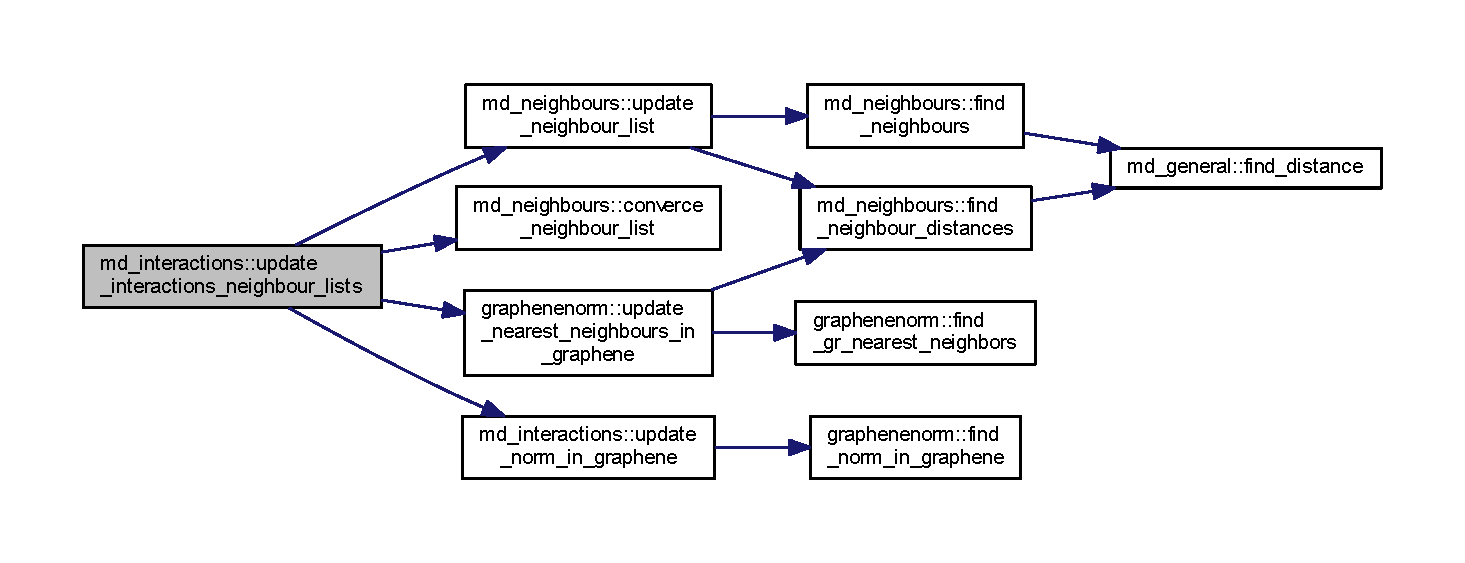
\includegraphics[width=350pt]{namespacemd__interactions_a311e6b53338f1b89611eec1929a6387e_cgraph}
\end{center}
\end{figure}
\mbox{\Hypertarget{namespacemd__interactions_a0f767aead142dc9f1f692172a21a590a}\label{namespacemd__interactions_a0f767aead142dc9f1f692172a21a590a}} 
\index{md\+\_\+interactions@{md\+\_\+interactions}!update\+\_\+norm\+\_\+in\+\_\+graphene@{update\+\_\+norm\+\_\+in\+\_\+graphene}}
\index{update\+\_\+norm\+\_\+in\+\_\+graphene@{update\+\_\+norm\+\_\+in\+\_\+graphene}!md\+\_\+interactions@{md\+\_\+interactions}}
\subsubsection{\texorpdfstring{update\+\_\+norm\+\_\+in\+\_\+graphene()}{update\_norm\_in\_graphene()}}
{\footnotesize\ttfamily subroutine md\+\_\+interactions\+::update\+\_\+norm\+\_\+in\+\_\+graphene (\begin{DoxyParamCaption}\item[{type(\mbox{\hyperlink{structmd__interactions_1_1interaction}{interaction}}), dimension(\+:)}]{interactions }\end{DoxyParamCaption})}



См. определение в файле md\+\_\+interactions.\+f90 строка 196


\begin{DoxyCode}
196     \textcolor{keywordtype}{type}(interaction):: interactions(:)
197     \textcolor{keywordtype}{integer}:: i
198     
199     \textcolor{keywordflow}{do} i=1,\textcolor{keyword}{size}(interactions)
200         \textcolor{keywordflow}{select case} (interactions(i)%interaction\_name)
201         \textcolor{keywordflow}{case}(\textcolor{stringliteral}{'ljc'})
202             \textcolor{keyword}{call }find\_norm\_in\_graphene(interactions(i)%parameters%LJC(1)%gr\_norm,interactions(i)%nl(3)%dr)
203         \textcolor{keywordflow}{case}(\textcolor{stringliteral}{'morsec'})
204             \textcolor{keyword}{call }find\_norm\_in\_graphene(interactions(i)%parameters%MorseC(1)%gr\_norm,interactions(i)%nl(3)
      %dr)
205 \textcolor{keywordflow}{        end select}
206 \textcolor{keywordflow}{    enddo}
207 
\end{DoxyCode}
Граф вызовов\+:\nopagebreak
\begin{figure}[H]
\begin{center}
\leavevmode
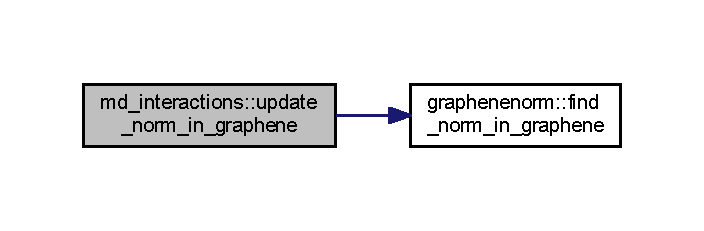
\includegraphics[width=338pt]{namespacemd__interactions_a0f767aead142dc9f1f692172a21a590a_cgraph}
\end{center}
\end{figure}

\hypertarget{namespacemd__neighbours}{}\section{Модуль md\+\_\+neighbours}
\label{namespacemd__neighbours}\index{md\+\_\+neighbours@{md\+\_\+neighbours}}


Модуль содержит подпрограммы относящиеся к спискам соседей частиц  


\subsection*{Функции/подпрограммы}
\begin{DoxyCompactItemize}
\item 
subroutine \mbox{\hyperlink{namespacemd__neighbours_a7246ea26ccbca29fb308ef82c2740bc9}{create\+\_\+neighbour\+\_\+list}} (nl)
\begin{DoxyCompactList}\small\item\em Инициализирует пустой список соседей. \end{DoxyCompactList}\item 
subroutine \mbox{\hyperlink{namespacemd__neighbours_aa3afc442e82c37b20e8963af79455747}{update\+\_\+neighbour\+\_\+list}} (md\+\_\+step, nl, atoms, group1, group2, box, exe\+\_\+time\+\_\+nlsearch, exe\+\_\+time\+\_\+nldistance)
\begin{DoxyCompactList}\small\item\em Вычисляет расстояния между соседями. Обновляет список соседей с нужной частотой.  Расстояния между соседями вычисляются всегда. Список соседей обнавляется с периодом указанным в списке. Также замеряется затраченное время. \end{DoxyCompactList}\item 
subroutine \mbox{\hyperlink{namespacemd__neighbours_a037f048abc67c7d83799c76aabaa8dac}{find\+\_\+neighbours}} (nl, atoms, group1, group2, box)
\begin{DoxyCompactList}\small\item\em Ищет соседей для частиц из первой группы среди второй группы.  Группы могут совпадать. \end{DoxyCompactList}\item 
subroutine \mbox{\hyperlink{namespacemd__neighbours_ad313293c81b7fa1b52e8376710c84c0f}{find\+\_\+neighbour\+\_\+distances}} (nl, atoms, group1, group2, box)
\begin{DoxyCompactList}\small\item\em Пересчитывает взаимное расположение соседей. \end{DoxyCompactList}\item 
subroutine \mbox{\hyperlink{namespacemd__neighbours_a3f6d619145cba9b77814f398056c243f}{converce\+\_\+neighbour\+\_\+list}} (cnl, group2, nl)
\begin{DoxyCompactList}\small\item\em Делает список соседей для второй группы из списка соседей для первой группы.  Эквивалентно find\+\_\+neighbours(сnl,atoms,group2,group1,box). Обращенный список соседей заполняется данными из списка полученного подпрогаммой find\+\_\+neighbours(nl,atoms,group1,group2,box) \end{DoxyCompactList}\end{DoxyCompactItemize}


\subsection{Подробное описание}
Модуль содержит подпрограммы относящиеся к спискам соседей частиц 

\subsection{Функции/подпрограммы}
\mbox{\Hypertarget{namespacemd__neighbours_a3f6d619145cba9b77814f398056c243f}\label{namespacemd__neighbours_a3f6d619145cba9b77814f398056c243f}} 
\index{md\+\_\+neighbours@{md\+\_\+neighbours}!converce\+\_\+neighbour\+\_\+list@{converce\+\_\+neighbour\+\_\+list}}
\index{converce\+\_\+neighbour\+\_\+list@{converce\+\_\+neighbour\+\_\+list}!md\+\_\+neighbours@{md\+\_\+neighbours}}
\subsubsection{\texorpdfstring{converce\+\_\+neighbour\+\_\+list()}{converce\_neighbour\_list()}}
{\footnotesize\ttfamily subroutine md\+\_\+neighbours\+::converce\+\_\+neighbour\+\_\+list (\begin{DoxyParamCaption}\item[{type(\mbox{\hyperlink{structmd__general_1_1neighbour__list}{neighbour\+\_\+list}})}]{cnl,  }\item[{type(\mbox{\hyperlink{structmd__general_1_1particle__group}{particle\+\_\+group}})}]{group2,  }\item[{type(\mbox{\hyperlink{structmd__general_1_1neighbour__list}{neighbour\+\_\+list}})}]{nl }\end{DoxyParamCaption})}



Делает список соседей для второй группы из списка соседей для первой группы.  Эквивалентно find\+\_\+neighbours(сnl,atoms,group2,group1,box). Обращенный список соседей заполняется данными из списка полученного подпрогаммой find\+\_\+neighbours(nl,atoms,group1,group2,box) 



См. определение в файле md\+\_\+neighbours.\+f90 строка 129


\begin{DoxyCode}
129     \textcolor{keywordtype}{type}(neighbour\_list):: nl,cnl
130     \textcolor{keywordtype}{type}(particle\_group):: group2
131     \textcolor{keywordtype}{integer}::       i,j,p
132     
133     \textcolor{keywordflow}{if} (group2%N>0 .and. nl%N>0 .and. cnl%N>0) \textcolor{keywordflow}{then}
134         \textcolor{keywordflow}{if} (group2%N>cnl%N) then; \textcolor{keyword}{write}(*,*) \textcolor{stringliteral}{'error: group2%N>cnl%N'},group2%N,cnl%N; stop;\textcolor{keywordflow}{ endif}
135         \textcolor{comment}{!$OMP PARALLEL firstprivate(i)}
136         \textcolor{comment}{!$OMP DO}
137         \textcolor{keywordflow}{do} i=1,group2%N
138             cnl%particle\_index(i) = group2%indexes(i)
139 \textcolor{keywordflow}{        enddo}
140         \textcolor{comment}{!$OMP END DO}
141         \textcolor{comment}{!$OMP DO}
142         \textcolor{keywordflow}{do} i=1,cnl%N
143             cnl%nnum(i) = 0
144 \textcolor{keywordflow}{        enddo}
145         \textcolor{comment}{!$OMP END DO}
146         \textcolor{comment}{!$OMP END PARALLEL}
147         \textcolor{keywordflow}{do} i=1,nl%N \textcolor{comment}{!can not be parallel!}
148             \textcolor{keywordflow}{do} p=1,nl%nnum(i)
149                 j = nl%nlist(p,i)
150                 cnl%nnum(j) = cnl%nnum(j)+1
151                 \textcolor{keywordflow}{if} (cnl%nnum(j)>cnl%neighb\_num\_max) then; \textcolor{keyword}{write}(*,*) \textcolor{stringliteral}{'error: too many neighbours'},j,cnl
      %nnum(j); stop;\textcolor{keywordflow}{ endif}
152                 cnl%nlist(cnl%nnum(j),j) = i
153                 cnl%dr(:,cnl%nnum(j),j) = -nl%dr(:,p,i)
154                 cnl%moddr(cnl%nnum(j),j) = nl%moddr(p,i)
155 \textcolor{keywordflow}{            enddo}
156 \textcolor{keywordflow}{        enddo}
157 \textcolor{keywordflow}{    endif}
158     
159     \textcolor{keywordflow}{return}
\end{DoxyCode}
\mbox{\Hypertarget{namespacemd__neighbours_a7246ea26ccbca29fb308ef82c2740bc9}\label{namespacemd__neighbours_a7246ea26ccbca29fb308ef82c2740bc9}} 
\index{md\+\_\+neighbours@{md\+\_\+neighbours}!create\+\_\+neighbour\+\_\+list@{create\+\_\+neighbour\+\_\+list}}
\index{create\+\_\+neighbour\+\_\+list@{create\+\_\+neighbour\+\_\+list}!md\+\_\+neighbours@{md\+\_\+neighbours}}
\subsubsection{\texorpdfstring{create\+\_\+neighbour\+\_\+list()}{create\_neighbour\_list()}}
{\footnotesize\ttfamily subroutine md\+\_\+neighbours\+::create\+\_\+neighbour\+\_\+list (\begin{DoxyParamCaption}\item[{type(\mbox{\hyperlink{structmd__general_1_1neighbour__list}{neighbour\+\_\+list}})}]{nl }\end{DoxyParamCaption})}



Инициализирует пустой список соседей. 



См. определение в файле md\+\_\+neighbours.\+f90 строка 10


\begin{DoxyCode}
10     \textcolor{keywordtype}{type}(neighbour\_list):: nl
11 
12     \textcolor{keywordflow}{if} (nl%N>0) \textcolor{keywordflow}{then}
13         \textcolor{keyword}{allocate}(nl%particle\_index(nl%N))
14         \textcolor{keyword}{allocate}(nl%nnum(nl%N))
15         \textcolor{keyword}{allocate}(nl%lessnnum(nl%N))
16         \textcolor{keyword}{allocate}(nl%nlist(nl%neighb\_num\_max,nl%N))
17         \textcolor{keyword}{allocate}(nl%dr(3,nl%neighb\_num\_max,nl%N))
18         \textcolor{keyword}{allocate}(nl%moddr(nl%neighb\_num\_max,nl%N))
19         nl%particle\_index = 0
20         nl%nnum = 0
21         nl%lessnnum = 0
22         nl%nlist = 0
23         nl%dr = 0.
24         nl%moddr = 0.
25 \textcolor{keywordflow}{    endif}
26     
27     \textcolor{keywordflow}{return}
\end{DoxyCode}
\mbox{\Hypertarget{namespacemd__neighbours_ad313293c81b7fa1b52e8376710c84c0f}\label{namespacemd__neighbours_ad313293c81b7fa1b52e8376710c84c0f}} 
\index{md\+\_\+neighbours@{md\+\_\+neighbours}!find\+\_\+neighbour\+\_\+distances@{find\+\_\+neighbour\+\_\+distances}}
\index{find\+\_\+neighbour\+\_\+distances@{find\+\_\+neighbour\+\_\+distances}!md\+\_\+neighbours@{md\+\_\+neighbours}}
\subsubsection{\texorpdfstring{find\+\_\+neighbour\+\_\+distances()}{find\_neighbour\_distances()}}
{\footnotesize\ttfamily subroutine md\+\_\+neighbours\+::find\+\_\+neighbour\+\_\+distances (\begin{DoxyParamCaption}\item[{type(\mbox{\hyperlink{structmd__general_1_1neighbour__list}{neighbour\+\_\+list}})}]{nl,  }\item[{type(\mbox{\hyperlink{structmd__general_1_1particles}{particles}})}]{atoms,  }\item[{type(\mbox{\hyperlink{structmd__general_1_1particle__group}{particle\+\_\+group}})}]{group1,  }\item[{type(\mbox{\hyperlink{structmd__general_1_1particle__group}{particle\+\_\+group}})}]{group2,  }\item[{type(\mbox{\hyperlink{structmd__general_1_1simulation__cell}{simulation\+\_\+cell}})}]{box }\end{DoxyParamCaption})}



Пересчитывает взаимное расположение соседей. 

\begin{DoxyRefDesc}{Необходимо сделать}
\item[\mbox{\hyperlink{todo__todo000001}{Необходимо сделать}}]Сделать sqrt(dr2) быстрее. \end{DoxyRefDesc}


См. определение в файле md\+\_\+neighbours.\+f90 строка 105


\begin{DoxyCode}
105     \textcolor{keywordtype}{type}(particles)::   atoms
106     \textcolor{keywordtype}{type}(particle\_group):: group1,group2
107     \textcolor{keywordtype}{type}(simulation\_cell):: box
108     \textcolor{keywordtype}{type}(neighbour\_list):: nl
109     \textcolor{keywordtype}{real}:: dr2
110     \textcolor{keywordtype}{integer}:: i,p
111 
112     \textcolor{comment}{!$OMP PARALLEL firstprivate(i,p,dr2)}
113     \textcolor{comment}{!$OMP DO}
114     \textcolor{keywordflow}{do} i=1,nl%N
115         \textcolor{keywordflow}{do} p=1,nl%nnum(i)
116             \textcolor{keyword}{call }find\_distance(nl%dr(:,p,i),dr2,atoms%positions(:,group1%indexes(i)),atoms%positions(:,
      group2%indexes(nl%nlist(p,i))),box)
117             nl%moddr(p,i) = sqrt(dr2)
118 \textcolor{keywordflow}{        enddo}
119 \textcolor{keywordflow}{    enddo}
120     \textcolor{comment}{!$OMP END DO}
121     \textcolor{comment}{!$OMP END PARALLEL}
122 
123     \textcolor{keywordflow}{return}
\end{DoxyCode}
Граф вызовов\+:\nopagebreak
\begin{figure}[H]
\begin{center}
\leavevmode
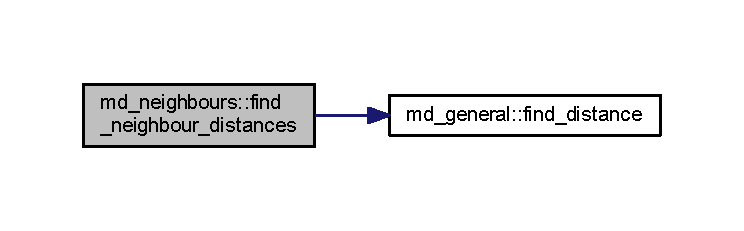
\includegraphics[width=350pt]{namespacemd__neighbours_ad313293c81b7fa1b52e8376710c84c0f_cgraph}
\end{center}
\end{figure}
\mbox{\Hypertarget{namespacemd__neighbours_a037f048abc67c7d83799c76aabaa8dac}\label{namespacemd__neighbours_a037f048abc67c7d83799c76aabaa8dac}} 
\index{md\+\_\+neighbours@{md\+\_\+neighbours}!find\+\_\+neighbours@{find\+\_\+neighbours}}
\index{find\+\_\+neighbours@{find\+\_\+neighbours}!md\+\_\+neighbours@{md\+\_\+neighbours}}
\subsubsection{\texorpdfstring{find\+\_\+neighbours()}{find\_neighbours()}}
{\footnotesize\ttfamily subroutine md\+\_\+neighbours\+::find\+\_\+neighbours (\begin{DoxyParamCaption}\item[{type(\mbox{\hyperlink{structmd__general_1_1neighbour__list}{neighbour\+\_\+list}})}]{nl,  }\item[{type(\mbox{\hyperlink{structmd__general_1_1particles}{particles}})}]{atoms,  }\item[{type(\mbox{\hyperlink{structmd__general_1_1particle__group}{particle\+\_\+group}})}]{group1,  }\item[{type(\mbox{\hyperlink{structmd__general_1_1particle__group}{particle\+\_\+group}})}]{group2,  }\item[{type(\mbox{\hyperlink{structmd__general_1_1simulation__cell}{simulation\+\_\+cell}})}]{box }\end{DoxyParamCaption})}



Ищет соседей для частиц из первой группы среди второй группы.  Группы могут совпадать. 



См. определение в файле md\+\_\+neighbours.\+f90 строка 57


\begin{DoxyCode}
57     \textcolor{keywordtype}{type}(particles)::   atoms
58     \textcolor{keywordtype}{type}(particle\_group):: group1,group2
59     \textcolor{keywordtype}{type}(simulation\_cell):: box
60     \textcolor{keywordtype}{type}(neighbour\_list):: nl
61     \textcolor{keywordtype}{real}:: dr(3),dr2
62     \textcolor{keywordtype}{integer}:: i,j,k,ind,jnd,nnumind,lessnnumind
63     
64     \textcolor{keywordflow}{if} (group1%N>nl%N) then; \textcolor{keyword}{write}(*,*) \textcolor{stringliteral}{'error: group1%N>nl%N'},group1%N,nl%N; stop;\textcolor{keywordflow}{ endif}
65     \textcolor{comment}{!$OMP PARALLEL firstprivate(i,j,k,ind,jnd,dr,dr2,nnumind,lessnnumind)}
66     \textcolor{comment}{!$OMP DO}
67     \textcolor{keywordflow}{do} ind=1,group1%N
68         i = group1%indexes(ind)
69         nl%particle\_index(ind) = group1%indexes(ind)
70         \textcolor{comment}{!nl%nlist(:nl%nnum(ind),ind) = 0}
71         nnumind = 0
72         lessnnumind = -1
73         \textcolor{keywordflow}{do} jnd=1,group2%N
74             j = group2%indexes(jnd)
75             \textcolor{keywordflow}{if} (i/=j) \textcolor{keywordflow}{then}
76                 \textcolor{keyword}{call }find\_distance(dr,dr2,atoms%positions(:,i),atoms%positions(:,j),box)
77                 \textcolor{keywordflow}{if} (dr2<nl%r\_cut*nl%r\_cut) \textcolor{keywordflow}{then}
78                     \textcolor{keywordflow}{if} (lessnnumind==-1 .and. i<j) lessnnumind = nnumind
79                     nnumind = nnumind+1
80                     \textcolor{keywordflow}{if} (nnumind>nl%neighb\_num\_max) then; \textcolor{keyword}{write}(*,*) \textcolor{stringliteral}{'error: too many neighbours'},ind,
      nnumind; stop;\textcolor{keywordflow}{ endif}
81                     nl%nlist(nnumind,ind) = jnd
82                     nl%dr(1,nnumind,ind) = dr(1)
83                     nl%dr(2,nnumind,ind) = dr(2)
84                     nl%dr(3,nnumind,ind) = dr(3)
85                     nl%moddr(nnumind,ind) = sqrt(dr2)
86 \textcolor{keywordflow}{                endif}
87 \textcolor{keywordflow}{            endif}
88 \textcolor{keywordflow}{        enddo}
89         \textcolor{keywordflow}{if}(lessnnumind==-1) \textcolor{keywordflow}{then}
90             nl%lessnnum(ind) = nnumind
91         \textcolor{keywordflow}{else}
92             nl%lessnnum(ind) = lessnnumind
93 \textcolor{keywordflow}{        endif}
94         nl%nnum(ind) = nnumind
95 \textcolor{keywordflow}{    enddo}
96     \textcolor{comment}{!$OMP END DO}
97     \textcolor{comment}{!$OMP END PARALLEL}
98 
99     \textcolor{keywordflow}{return}
\end{DoxyCode}
Граф вызовов\+:\nopagebreak
\begin{figure}[H]
\begin{center}
\leavevmode
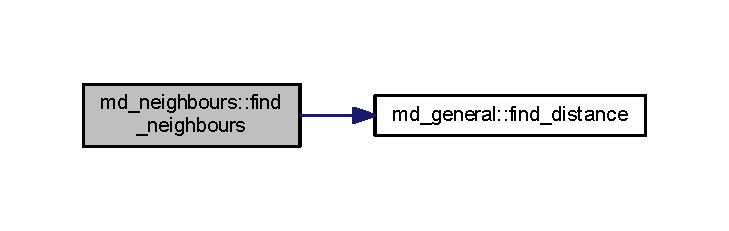
\includegraphics[width=350pt]{namespacemd__neighbours_a037f048abc67c7d83799c76aabaa8dac_cgraph}
\end{center}
\end{figure}
\mbox{\Hypertarget{namespacemd__neighbours_aa3afc442e82c37b20e8963af79455747}\label{namespacemd__neighbours_aa3afc442e82c37b20e8963af79455747}} 
\index{md\+\_\+neighbours@{md\+\_\+neighbours}!update\+\_\+neighbour\+\_\+list@{update\+\_\+neighbour\+\_\+list}}
\index{update\+\_\+neighbour\+\_\+list@{update\+\_\+neighbour\+\_\+list}!md\+\_\+neighbours@{md\+\_\+neighbours}}
\subsubsection{\texorpdfstring{update\+\_\+neighbour\+\_\+list()}{update\_neighbour\_list()}}
{\footnotesize\ttfamily subroutine md\+\_\+neighbours\+::update\+\_\+neighbour\+\_\+list (\begin{DoxyParamCaption}\item[{integer}]{md\+\_\+step,  }\item[{type(\mbox{\hyperlink{structmd__general_1_1neighbour__list}{neighbour\+\_\+list}})}]{nl,  }\item[{type(\mbox{\hyperlink{structmd__general_1_1particles}{particles}})}]{atoms,  }\item[{type(\mbox{\hyperlink{structmd__general_1_1particle__group}{particle\+\_\+group}})}]{group1,  }\item[{type(\mbox{\hyperlink{structmd__general_1_1particle__group}{particle\+\_\+group}})}]{group2,  }\item[{type(\mbox{\hyperlink{structmd__general_1_1simulation__cell}{simulation\+\_\+cell}})}]{box,  }\item[{real}]{exe\+\_\+time\+\_\+nlsearch,  }\item[{real}]{exe\+\_\+time\+\_\+nldistance }\end{DoxyParamCaption})}



Вычисляет расстояния между соседями. Обновляет список соседей с нужной частотой.  Расстояния между соседями вычисляются всегда. Список соседей обнавляется с периодом указанным в списке. Также замеряется затраченное время. 



См. определение в файле md\+\_\+neighbours.\+f90 строка 33


\begin{DoxyCode}
33     \textcolor{keywordtype}{type}(particles)::   atoms
34     \textcolor{keywordtype}{type}(particle\_group):: group1,group2
35     \textcolor{keywordtype}{type}(simulation\_cell):: box
36     \textcolor{keywordtype}{type}(neighbour\_list):: nl
37     \textcolor{keywordtype}{integer}:: md\_step
38     \textcolor{keywordtype}{real}:: exe\_t,exe\_time\_nlsearch,exe\_time\_nldistance,omp\_get\_wtime
39 
40     \textcolor{keywordflow}{if} (group1%N>0 .and. group2%N>0 .and. nl%N>0) \textcolor{keywordflow}{then}
41         \textcolor{keywordflow}{if} (mod(md\_step,nl%update\_period)==0) \textcolor{keywordflow}{then}
42             exe\_t = omp\_get\_wtime()
43             \textcolor{keyword}{call }find\_neighbours(nl,atoms,group1,group2,box)
44             exe\_time\_nlsearch = exe\_time\_nlsearch+omp\_get\_wtime()-exe\_t
45         \textcolor{keywordflow}{else}
46             exe\_t = omp\_get\_wtime()
47             \textcolor{keyword}{call }find\_neighbour\_distances(nl,atoms,group1,group2,box)
48             exe\_time\_nldistance = exe\_time\_nldistance+omp\_get\_wtime()-exe\_t
49 \textcolor{keywordflow}{        endif}
50 \textcolor{keywordflow}{    endif}
51     
\end{DoxyCode}
Граф вызовов\+:\nopagebreak
\begin{figure}[H]
\begin{center}
\leavevmode
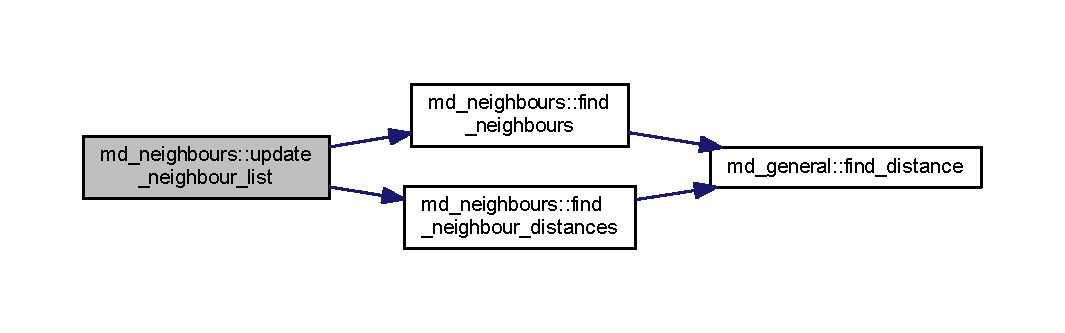
\includegraphics[width=350pt]{namespacemd__neighbours_aa3afc442e82c37b20e8963af79455747_cgraph}
\end{center}
\end{figure}

\hypertarget{namespacemd__read__write}{}\section{Модуль md\+\_\+read\+\_\+write}
\label{namespacemd__read__write}\index{md\+\_\+read\+\_\+write@{md\+\_\+read\+\_\+write}}


Модуль ввода вывода .xyz файлов и настроек моделирования.  


\subsection*{Функции/подпрограммы}
\begin{DoxyCompactItemize}
\item 
subroutine \mbox{\hyperlink{namespacemd__read__write_a13e739c9b44b3100ee36e864eac3d5e0}{read\+\_\+integrator\+\_\+params}} (integr, file\+\_\+id)
\begin{DoxyCompactList}\small\item\em Читает параметры интегратора. \end{DoxyCompactList}\item 
subroutine \mbox{\hyperlink{namespacemd__read__write_ace09a29b4fd526f8ed784c90098279c4}{read\+\_\+box\+\_\+size}} (box, filename)
\begin{DoxyCompactList}\small\item\em Читает параметры моделируемой ячейки в файле .xyz.  Читает второю строку в xyz файле. В размер ячейки задается тремя векторами. В общем случае ячейка триклинная. \end{DoxyCompactList}\item 
subroutine \mbox{\hyperlink{namespacemd__read__write_a1a0fd7df876318fd4247d110936384d8}{read\+\_\+particles}} (atoms, filename)
\begin{DoxyCompactList}\small\item\em Читает информацию о частицах из .xyz файла.  Первая строка файла содержит количество частиц. Третья и последующие -\/ координаты по X, Y, Z, скорости по X, Y, Z, массу и название частицы. Всего 8 столбцов для каждой частицы. \end{DoxyCompactList}\item 
subroutine \mbox{\hyperlink{namespacemd__read__write_a20f73c896cf124f2e1da6ccbf23cc12d}{write\+\_\+particle\+\_\+group}} (filename, atoms, group, box)
\begin{DoxyCompactList}\small\item\em Выводит информацию о группе частиц в новый файл. \end{DoxyCompactList}\item 
subroutine \mbox{\hyperlink{namespacemd__read__write_a24453b47bb1935e66563cd522e09e3af}{write\+\_\+particle\+\_\+group\+\_\+append}} (filename, atoms, group, box, md\+\_\+step)
\begin{DoxyCompactList}\small\item\em Выводит информацию о группе частиц в конец уже имеющегося файла. \end{DoxyCompactList}\end{DoxyCompactItemize}


\subsection{Подробное описание}
Модуль ввода вывода .xyz файлов и настроек моделирования. 

\begin{DoxyRefDesc}{Необходимо сделать}
\item[\mbox{\hyperlink{todo__todo000002}{Необходимо сделать}}]Добавить чтение файла настроек. \end{DoxyRefDesc}


\subsection{Функции/подпрограммы}
\mbox{\Hypertarget{namespacemd__read__write_ace09a29b4fd526f8ed784c90098279c4}\label{namespacemd__read__write_ace09a29b4fd526f8ed784c90098279c4}} 
\index{md\+\_\+read\+\_\+write@{md\+\_\+read\+\_\+write}!read\+\_\+box\+\_\+size@{read\+\_\+box\+\_\+size}}
\index{read\+\_\+box\+\_\+size@{read\+\_\+box\+\_\+size}!md\+\_\+read\+\_\+write@{md\+\_\+read\+\_\+write}}
\subsubsection{\texorpdfstring{read\+\_\+box\+\_\+size()}{read\_box\_size()}}
{\footnotesize\ttfamily subroutine md\+\_\+read\+\_\+write\+::read\+\_\+box\+\_\+size (\begin{DoxyParamCaption}\item[{type(\mbox{\hyperlink{structmd__general_1_1simulation__cell}{simulation\+\_\+cell}})}]{box,  }\item[{character($\ast$)}]{filename }\end{DoxyParamCaption})}



Читает параметры моделируемой ячейки в файле .xyz.  Читает второю строку в xyz файле. В размер ячейки задается тремя векторами. В общем случае ячейка триклинная. 

\begin{DoxyWarning}{Предупреждения}
Данная подпрограмма (как и вся программа) рассчитана только на прямоугольные ячейки. 
\end{DoxyWarning}


См. определение в файле md\+\_\+read\+\_\+write.\+f90 строка 23


\begin{DoxyCode}
23     \textcolor{keywordtype}{type}(simulation\_cell):: box
24     \textcolor{keywordtype}{real}:: boxmatrix(9)
25     \textcolor{keywordtype}{character(*)}::  filename
26     \textcolor{keywordtype}{character(len=32)}:: c
27 
28     \textcolor{keyword}{open}(1,file=filename)
29     \textcolor{keyword}{read}(1,*)
30     \textcolor{keyword}{read}(1,*) c,boxmatrix
31     \textcolor{keyword}{close}(1)
32     box%box\_size(1)=boxmatrix(1)
33     box%box\_size(2)=boxmatrix(5)
34     box%box\_size(3)=boxmatrix(9)
35     box%half\_box\_size = 0.5*box%box\_size
36     
37     \textcolor{keywordflow}{return}
\end{DoxyCode}
\mbox{\Hypertarget{namespacemd__read__write_a13e739c9b44b3100ee36e864eac3d5e0}\label{namespacemd__read__write_a13e739c9b44b3100ee36e864eac3d5e0}} 
\index{md\+\_\+read\+\_\+write@{md\+\_\+read\+\_\+write}!read\+\_\+integrator\+\_\+params@{read\+\_\+integrator\+\_\+params}}
\index{read\+\_\+integrator\+\_\+params@{read\+\_\+integrator\+\_\+params}!md\+\_\+read\+\_\+write@{md\+\_\+read\+\_\+write}}
\subsubsection{\texorpdfstring{read\+\_\+integrator\+\_\+params()}{read\_integrator\_params()}}
{\footnotesize\ttfamily subroutine md\+\_\+read\+\_\+write\+::read\+\_\+integrator\+\_\+params (\begin{DoxyParamCaption}\item[{type(\mbox{\hyperlink{structmd__general_1_1integrator__params}{integrator\+\_\+params}})}]{integr,  }\item[{integer}]{file\+\_\+id }\end{DoxyParamCaption})}



Читает параметры интегратора. 



См. определение в файле md\+\_\+read\+\_\+write.\+f90 строка 11


\begin{DoxyCode}
11     \textcolor{keywordtype}{type}(integrator\_params):: integr
12     \textcolor{keywordtype}{integer}:: file\_id 
13 
14     \textcolor{keyword}{read}(file\_id,*) integr%int\_name,integr%dt,integr%l,integr%period\_snapshot,integr%period\_log
15 
16     \textcolor{keywordflow}{return}
\end{DoxyCode}
\mbox{\Hypertarget{namespacemd__read__write_a1a0fd7df876318fd4247d110936384d8}\label{namespacemd__read__write_a1a0fd7df876318fd4247d110936384d8}} 
\index{md\+\_\+read\+\_\+write@{md\+\_\+read\+\_\+write}!read\+\_\+particles@{read\+\_\+particles}}
\index{read\+\_\+particles@{read\+\_\+particles}!md\+\_\+read\+\_\+write@{md\+\_\+read\+\_\+write}}
\subsubsection{\texorpdfstring{read\+\_\+particles()}{read\_particles()}}
{\footnotesize\ttfamily subroutine md\+\_\+read\+\_\+write\+::read\+\_\+particles (\begin{DoxyParamCaption}\item[{type(\mbox{\hyperlink{structmd__general_1_1particles}{particles}})}]{atoms,  }\item[{character($\ast$)}]{filename }\end{DoxyParamCaption})}



Читает информацию о частицах из .xyz файла.  Первая строка файла содержит количество частиц. Третья и последующие -\/ координаты по X, Y, Z, скорости по X, Y, Z, массу и название частицы. Всего 8 столбцов для каждой частицы. 



См. определение в файле md\+\_\+read\+\_\+write.\+f90 строка 43


\begin{DoxyCode}
43     \textcolor{keywordtype}{type}(particles)::   atoms
44     \textcolor{keywordtype}{character(*)}::  filename
45     \textcolor{keywordtype}{integer}::       i
46 
47     \textcolor{keyword}{open}(1,file=filename)
48     \textcolor{keyword}{read}(1,*) atoms%N
49     \textcolor{keyword}{allocate}(atoms%positions(3,atoms%N))
50     \textcolor{keyword}{allocate}(atoms%velocities(3,atoms%N))
51     \textcolor{keyword}{allocate}(atoms%forces(3,atoms%N))
52     \textcolor{keyword}{allocate}(atoms%masses(atoms%N))
53     \textcolor{keyword}{allocate}(atoms%atom\_types(atoms%N))
54     \textcolor{keyword}{read}(1,*)
55     \textcolor{keywordflow}{do} i=1,atoms%N
56         \textcolor{keyword}{read}(1,*) atoms%positions(:,i),atoms%velocities(:,i),atoms%masses(i),atoms%atom\_types(i)
57 \textcolor{keywordflow}{    enddo}
58     \textcolor{keyword}{close}(1)
59 
60     \textcolor{keywordflow}{return}
\end{DoxyCode}
\mbox{\Hypertarget{namespacemd__read__write_a20f73c896cf124f2e1da6ccbf23cc12d}\label{namespacemd__read__write_a20f73c896cf124f2e1da6ccbf23cc12d}} 
\index{md\+\_\+read\+\_\+write@{md\+\_\+read\+\_\+write}!write\+\_\+particle\+\_\+group@{write\+\_\+particle\+\_\+group}}
\index{write\+\_\+particle\+\_\+group@{write\+\_\+particle\+\_\+group}!md\+\_\+read\+\_\+write@{md\+\_\+read\+\_\+write}}
\subsubsection{\texorpdfstring{write\+\_\+particle\+\_\+group()}{write\_particle\_group()}}
{\footnotesize\ttfamily subroutine md\+\_\+read\+\_\+write\+::write\+\_\+particle\+\_\+group (\begin{DoxyParamCaption}\item[{character($\ast$)}]{filename,  }\item[{type(\mbox{\hyperlink{structmd__general_1_1particles}{particles}})}]{atoms,  }\item[{type(\mbox{\hyperlink{structmd__general_1_1particle__group}{particle\+\_\+group}})}]{group,  }\item[{type(\mbox{\hyperlink{structmd__general_1_1simulation__cell}{simulation\+\_\+cell}})}]{box }\end{DoxyParamCaption})}



Выводит информацию о группе частиц в новый файл. 

\begin{DoxyWarning}{Предупреждения}
Если файл с таким именем уже существует, он будет заменен новым. 
\end{DoxyWarning}


См. определение в файле md\+\_\+read\+\_\+write.\+f90 строка 66


\begin{DoxyCode}
66     \textcolor{keywordtype}{type}(particles)::   atoms
67     \textcolor{keywordtype}{type}(particle\_group)::  group
68     \textcolor{keywordtype}{type}(simulation\_cell):: box
69     \textcolor{keywordtype}{character(*)}::  filename
70     \textcolor{keywordtype}{integer}::       i,ind
71 
72     \textcolor{keyword}{open}(2,file=filename)
73     \textcolor{keyword}{write}(2,*) group%N
74     \textcolor{keyword}{write}(2,\textcolor{stringliteral}{'(A,9f16.6,A)'}) \textcolor{stringliteral}{'Lattice="'},box%box\_size(1), 0., 0., 0., box%box\_size(2), 0., 0., 0., box
      %box\_size(3),&
75             \textcolor{stringliteral}{' " Properties=pos:R:3:vel:R:3:mass:R:1:species:S:1'}
76     \textcolor{keywordflow}{do} ind=1,group%N
77         i = group%indexes(ind)
78         \textcolor{keyword}{write}(2,\textcolor{stringliteral}{'(7f27.16,A,A)'}) atoms%positions(:,i),atoms%velocities(:,i),atoms%masses(i),\textcolor{stringliteral}{'    '},atoms
      %atom\_types(i)
79 \textcolor{keywordflow}{    enddo}
80     \textcolor{keyword}{close}(2)
81 
82     \textcolor{keywordflow}{return}
\end{DoxyCode}
\mbox{\Hypertarget{namespacemd__read__write_a24453b47bb1935e66563cd522e09e3af}\label{namespacemd__read__write_a24453b47bb1935e66563cd522e09e3af}} 
\index{md\+\_\+read\+\_\+write@{md\+\_\+read\+\_\+write}!write\+\_\+particle\+\_\+group\+\_\+append@{write\+\_\+particle\+\_\+group\+\_\+append}}
\index{write\+\_\+particle\+\_\+group\+\_\+append@{write\+\_\+particle\+\_\+group\+\_\+append}!md\+\_\+read\+\_\+write@{md\+\_\+read\+\_\+write}}
\subsubsection{\texorpdfstring{write\+\_\+particle\+\_\+group\+\_\+append()}{write\_particle\_group\_append()}}
{\footnotesize\ttfamily subroutine md\+\_\+read\+\_\+write\+::write\+\_\+particle\+\_\+group\+\_\+append (\begin{DoxyParamCaption}\item[{character($\ast$)}]{filename,  }\item[{type(\mbox{\hyperlink{structmd__general_1_1particles}{particles}})}]{atoms,  }\item[{type(\mbox{\hyperlink{structmd__general_1_1particle__group}{particle\+\_\+group}})}]{group,  }\item[{type(\mbox{\hyperlink{structmd__general_1_1simulation__cell}{simulation\+\_\+cell}})}]{box,  }\item[{integer}]{md\+\_\+step }\end{DoxyParamCaption})}



Выводит информацию о группе частиц в конец уже имеющегося файла. 



См. определение в файле md\+\_\+read\+\_\+write.\+f90 строка 87


\begin{DoxyCode}
87     \textcolor{keywordtype}{type}(particles)::   atoms
88     \textcolor{keywordtype}{type}(particle\_group)::  group
89     \textcolor{keywordtype}{type}(simulation\_cell):: box
90     \textcolor{keywordtype}{character(*)}::  filename
91     \textcolor{keywordtype}{integer}::       i,ind,md\_step
92 
93     \textcolor{keywordflow}{if}(group%N>0) \textcolor{keywordflow}{then}
94         \textcolor{keyword}{open}(2,file=filename,action=\textcolor{stringliteral}{'write'},position=\textcolor{stringliteral}{'append'})
95         \textcolor{keyword}{write}(2,*) group%N
96         \textcolor{keyword}{write}(2,\textcolor{stringliteral}{'(A,i9,A,9f10.4,A)'}) \textcolor{stringliteral}{'time\_step: '},md\_step,&
97         \textcolor{stringliteral}{'    Lattice="'},box%box\_size(1), 0., 0., 0., box%box\_size(2), 0., 0., 0., box%box\_size(3),&
98         \textcolor{stringliteral}{' " Properties=pos:R:3:vel:R:3:mass:R:1:species:S:1'}
99         \textcolor{keywordflow}{do} ind=1,group%N
100             i = group%indexes(ind)
101             \textcolor{keyword}{write}(2,\textcolor{stringliteral}{'(7f10.4,A,A)'}) atoms%positions(:,i),atoms%velocities(:,i),atoms%masses(i),\textcolor{stringliteral}{'    '},trim(
      atoms%atom\_types(i))
102 \textcolor{keywordflow}{        enddo}
103         \textcolor{keyword}{close}(2)
104 \textcolor{keywordflow}{    endif}
105     
106     \textcolor{keywordflow}{return}
\end{DoxyCode}

\hypertarget{namespacemd__simulation}{}\section{Модуль md\+\_\+simulation}
\label{namespacemd__simulation}\index{md\+\_\+simulation@{md\+\_\+simulation}}
\subsection*{Функции/подпрограммы}
\begin{DoxyCompactItemize}
\item 
subroutine \mbox{\hyperlink{namespacemd__simulation_ab2107f3ca598f6a748991632633ee760}{md}} (out\+\_\+id, all\+\_\+out\+\_\+id, input\+\_\+path, settings\+\_\+filename, output\+\_\+prefix, out\+\_\+period, num\+\_\+of\+\_\+omp\+\_\+treads)
\end{DoxyCompactItemize}


\subsection{Функции/подпрограммы}
\mbox{\Hypertarget{namespacemd__simulation_ab2107f3ca598f6a748991632633ee760}\label{namespacemd__simulation_ab2107f3ca598f6a748991632633ee760}} 
\index{md\+\_\+simulation@{md\+\_\+simulation}!md@{md}}
\index{md@{md}!md\+\_\+simulation@{md\+\_\+simulation}}
\subsubsection{\texorpdfstring{md()}{md()}}
{\footnotesize\ttfamily subroutine md\+\_\+simulation\+::md (\begin{DoxyParamCaption}\item[{integer}]{out\+\_\+id,  }\item[{integer}]{all\+\_\+out\+\_\+id,  }\item[{character(len=128)}]{input\+\_\+path,  }\item[{character(len=128)}]{settings\+\_\+filename,  }\item[{character(len=128)}]{output\+\_\+prefix,  }\item[{integer}]{out\+\_\+period,  }\item[{integer}]{num\+\_\+of\+\_\+omp\+\_\+treads }\end{DoxyParamCaption})}



См. определение в файле md\+\_\+simulation.\+f90 строка 10


\begin{DoxyCode}
10 
11 \textcolor{keywordtype}{type}(simulation\_cell)                   :: cell
12 \textcolor{keywordtype}{type}(time\_steps)                        :: dt
13 \textcolor{keywordtype}{type}(particles)                         :: atoms
14 \textcolor{keywordtype}{type}(particle\_group),allocatable        :: groups(:)
15 \textcolor{keywordtype}{type}(interaction),allocatable           :: interactions(:)
16 \textcolor{keywordtype}{type}(integrator\_params),allocatable     :: integrators(:)
17 \textcolor{keywordtype}{type}(nose\_hoover\_chain)                 :: nhc
18 real                                    ::  exe\_t,exe\_time\_start,exe\_time\_md,exe\_time\_pos\_vel,&
19                                             exe\_time\_nlists,exe\_time\_nlsearch,exe\_time\_nldistance,
      exe\_time\_forces,exe\_time\_energy,&
20                                             conserved\_energy,total\_energy,kinetic\_energy,potential\_energy,
      prev\_potential\_energy,&
21                                             ms\_de,fs(3),mcv(3),mc(3),initial\_temperature,target\_temperature
      ,temperature,nhc\_q1
22 integer                                 ::  i,num\_of\_omp\_treads,md\_step,md\_step\_limit,integrators\_num,
      integrator\_index,&
23                                             file\_id,out\_id,log\_id,out\_period,all\_out\_id,&
24                                             all\_atoms\_group\_num,termo\_atoms\_group\_num,&
25                                             all\_moving\_atoms\_group\_num,xyz\_moving\_atoms\_group\_num,
      z\_moving\_atoms\_group\_num,&
26                                             traj\_group\_num,period\_traj,change\_group\_num,&
27                                             zero\_momentum\_period
28 \textcolor{keywordtype}{integer},allocatable                     ::  group\_change\_from(:),group\_change\_to(:),change\_ts1(:),
      change\_ts2(:),change\_frec(:)
29 \textcolor{keywordtype}{character}(len=128)                      ::  str,filename,logfilename,init\_xyz\_filename,input\_path,
      settings\_filename,output\_prefix
30 \textcolor{keywordtype}{character}(len=32)                       ::  integrator\_name,interactions\_energies\_format
31 \textcolor{keywordtype}{logical}                                 ::  new\_velocities,invert\_z\_vel
32 real                                    ::  omp\_get\_wtime
33     
34 exe\_time\_start = omp\_get\_wtime()
35 log\_id = 108
36 file\_id = 2017
37 
38 \textcolor{keyword}{open}(file\_id,file=trim(input\_path)//settings\_filename); \textcolor{keyword}{write}(out\_id,\textcolor{stringliteral}{'(A,A)'}) \textcolor{stringliteral}{'settings\_filename: '},trim(
      settings\_filename)
39 \textcolor{keyword}{read}(file\_id,*) str,md\_step\_limit;                      \textcolor{keyword}{write}(out\_id,\textcolor{stringliteral}{'(A32,i12)'}) str,md\_step\_limit
40 \textcolor{keyword}{read}(file\_id,*) str,logfilename;                        \textcolor{keyword}{write}(out\_id,\textcolor{stringliteral}{'(A32,A,A)'}) str,\textcolor{stringliteral}{' '},trim(logfilename)
41 \textcolor{keyword}{read}(file\_id,*) str,init\_xyz\_filename;                  \textcolor{keyword}{write}(out\_id,\textcolor{stringliteral}{'(A32,A,A)'}) str,\textcolor{stringliteral}{' '},trim(
      init\_xyz\_filename)
42 \textcolor{keyword}{call }read\_box\_size(cell,trim(input\_path)//init\_xyz\_filename);   \textcolor{keyword}{write}(out\_id,\textcolor{stringliteral}{'(A,3f16.6)'})  \textcolor{stringliteral}{'box\_size: '},
      cell%box\_size
43 \textcolor{keyword}{call }read\_particles(atoms,trim(input\_path)//init\_xyz\_filename); \textcolor{keyword}{write}(out\_id,\textcolor{stringliteral}{'(A,i12)'})     \textcolor{stringliteral}{'particles\_num:
       '},atoms%N
44 \textcolor{keyword}{read}(file\_id,*) str,new\_velocities;                     \textcolor{keyword}{write}(out\_id,\textcolor{stringliteral}{'(A32,l8)'}) str,new\_velocities
45 \textcolor{keyword}{read}(file\_id,*) str,zero\_momentum\_period;               \textcolor{keyword}{write}(out\_id,\textcolor{stringliteral}{'(A32,i12)'}) str,zero\_momentum\_period
46 \textcolor{keyword}{call }create\_groups(groups,file\_id,out\_id,atoms)
47 \textcolor{keyword}{read}(file\_id,*) str,all\_moving\_atoms\_group\_num;         \textcolor{keyword}{write}(out\_id,\textcolor{stringliteral}{'(A32,i12)'}) str,
      all\_moving\_atoms\_group\_num
48 \textcolor{keyword}{read}(file\_id,*) str,xyz\_moving\_atoms\_group\_num;         \textcolor{keyword}{write}(out\_id,\textcolor{stringliteral}{'(A32,i12)'}) str,
      xyz\_moving\_atoms\_group\_num
49 \textcolor{keyword}{read}(file\_id,*) str,z\_moving\_atoms\_group\_num;           \textcolor{keyword}{write}(out\_id,\textcolor{stringliteral}{'(A32,i12)'}) str,
      z\_moving\_atoms\_group\_num
50 \textcolor{keyword}{read}(file\_id,*) str,termo\_atoms\_group\_num;              \textcolor{keyword}{write}(out\_id,\textcolor{stringliteral}{'(A32,i12)'}) str,termo\_atoms\_group\_num
51 \textcolor{keyword}{read}(file\_id,*) str,all\_atoms\_group\_num;                \textcolor{keyword}{write}(out\_id,\textcolor{stringliteral}{'(A32,i12)'}) str,all\_atoms\_group\_num
52 \textcolor{keyword}{read}(file\_id,*) str,traj\_group\_num;                     \textcolor{keyword}{write}(out\_id,\textcolor{stringliteral}{'(A32,i12)'}) str,traj\_group\_num
53 \textcolor{keyword}{read}(file\_id,*) str,period\_traj;                        \textcolor{keyword}{write}(out\_id,\textcolor{stringliteral}{'(A32,i12)'}) str,period\_traj
54 \textcolor{keyword}{read}(file\_id,*) str,change\_group\_num;                   \textcolor{keyword}{write}(out\_id,\textcolor{stringliteral}{'(A32,i12)'}) str,change\_group\_num
55 \textcolor{keyword}{allocate}(group\_change\_from(change\_group\_num),group\_change\_to(change\_group\_num),&
56 change\_ts1(change\_group\_num),change\_ts2(change\_group\_num),change\_frec(change\_group\_num))
57 \textcolor{keywordflow}{do} i=1,change\_group\_num
58     \textcolor{keyword}{read}(file\_id,*) str,group\_change\_from(i),group\_change\_to(i);
59     \textcolor{keyword}{write}(out\_id,\textcolor{stringliteral}{'(A32,2i12)'}) str,group\_change\_from(i),group\_change\_to(i)
60     \textcolor{keyword}{read}(file\_id,*) str,change\_ts1(i),change\_ts2(i),change\_frec(i)
61     \textcolor{keyword}{write}(out\_id,\textcolor{stringliteral}{'(A32,3i12)'}) str,change\_ts1(i),change\_ts2(i),change\_frec(i)
62 \textcolor{keywordflow}{enddo}
63 \textcolor{keyword}{read}(file\_id,*) str,invert\_z\_vel;                       \textcolor{keyword}{write}(out\_id,\textcolor{stringliteral}{'(A32,l8)'}) str,invert\_z\_vel
64 \textcolor{keyword}{read}(file\_id,*) str,integrators\_num;                    \textcolor{keyword}{write}(out\_id,\textcolor{stringliteral}{'(A32,i12)'}) str,integrators\_num
65 \textcolor{keyword}{allocate}(integrators(0:integrators\_num)); integrators(0)%int\_name=\textcolor{stringliteral}{'none'}; integrators(0)%dt=0.; integrators
      (0)%l=0
66 \textcolor{keyword}{read}(file\_id,\textcolor{stringliteral}{'(A)'}) str;                                \textcolor{keyword}{write}(out\_id,\textcolor{stringliteral}{'(A)'}) str
67 \textcolor{keywordflow}{do} i=1,integrators\_num
68     \textcolor{keyword}{call }read\_integrator\_params(integrators(i),file\_id)
69     \textcolor{keyword}{write}(out\_id,\textcolor{stringliteral}{'(A,A6,f10.5,4i9)'}) \textcolor{stringliteral}{'  '},integrators(i)%int\_name,&
70     integrators(i)%dt,integrators(i)%l,integrators(i)%period\_snapshot,integrators(i)%period\_log
71 \textcolor{keywordflow}{enddo}
72 \textcolor{keyword}{read}(file\_id,*) str,ms\_de;                              \textcolor{keyword}{write}(out\_id,\textcolor{stringliteral}{'(A32,f16.6)'}) str,ms\_de
73 \textcolor{keyword}{read}(file\_id,*) str,target\_temperature,nhc%M,nhc\_q1;    \textcolor{keyword}{write}(out\_id,\textcolor{stringliteral}{'(A32,f16.6,i6,f16.6)'}) str,
      target\_temperature,nhc%M,nhc\_q1
74 \textcolor{keyword}{call }create\_nose\_hoover\_chain(nhc)
75 \textcolor{keyword}{read}(file\_id,*) str,initial\_temperature;                \textcolor{keyword}{write}(out\_id,\textcolor{stringliteral}{'(A32,f16.6)'}) str,initial\_temperature
76 \textcolor{keywordflow}{if} (initial\_temperature<0.) initial\_temperature=0.
77 \textcolor{keywordflow}{if} (new\_velocities) \textcolor{keyword}{call }set\_new\_temperature(atoms,groups(all\_moving\_atoms\_group\_num),initial\_temperature)
78 \textcolor{keyword}{call }create\_interactions(interactions,groups,file\_id,out\_id,input\_path)
79 \textcolor{keyword}{close}(file\_id)
80 
81 \textcolor{keyword}{write}(interactions\_energies\_format,\textcolor{stringliteral}{'("(",i0,"f20.9)")'}) \textcolor{keyword}{size}(interactions)
82 \textcolor{keyword}{write}(str,\textcolor{stringliteral}{'(A,A)'}) trim(output\_prefix),trim(logfilename)
83 \textcolor{keyword}{open}(log\_id,file=str)
84 \textcolor{keyword}{write}(out\_id,\textcolor{stringliteral}{'(A24,1f10.2,A)'}) \textcolor{stringliteral}{'PREPARATIONS TIME: '},omp\_get\_wtime()-exe\_time\_start,\textcolor{stringliteral}{' S '}
85 \textcolor{keyword}{write}(out\_id,\textcolor{stringliteral}{'(A24,i6,A)'}) \textcolor{stringliteral}{'RUNNING ON '},num\_of\_omp\_treads,\textcolor{stringliteral}{' OPENMP THREADS'}
86 \textcolor{keyword}{call }set\_openmp\_perfomance(num\_of\_omp\_treads,atoms%N)
87 exe\_time\_md = omp\_get\_wtime()
88 exe\_time\_pos\_vel = 0.
89 exe\_time\_nlists = 0.
90 exe\_time\_forces = 0.
91 exe\_time\_energy = 0.
92 integrator\_index = 0
93 dt%simulation\_time = 0.
94 
95 \textcolor{keywordflow}{do} md\_step=0,md\_step\_limit
96 
97     \textcolor{keywordflow}{do} i=1,change\_group\_num
98         \textcolor{keyword}{call }change\_particle\_group\_n(groups(group\_change\_to(i)),md\_step,change\_ts1(i),change\_ts2(i),&
99         change\_frec(i),groups(group\_change\_from(i)))
100 \textcolor{keywordflow}{    enddo}
101     
102     \textcolor{keywordflow}{if} (md\_step-1==sum(integrators(0:integrator\_index)%l) .or. integrator\_index==0) \textcolor{keywordflow}{then}
103         integrator\_index = integrator\_index+1
104         \textcolor{keywordflow}{do} i=integrator\_index,integrators\_num
105             \textcolor{keywordflow}{if} (integrators(i)%l>0) \textcolor{keywordflow}{then}
106                 integrator\_name = integrators(i)%int\_name
107                 \textcolor{keyword}{call }init\_time\_steps(dt,integrators(i)%dt)
108                 \textcolor{keywordflow}{if} (integrator\_name==\textcolor{stringliteral}{'nvt'}) \textcolor{keyword}{call }set\_nose\_hoover\_chain(nhc,target\_temperature,nhc\_q1,groups
      (termo\_atoms\_group\_num)%N)
109                 \textcolor{keywordflow}{exit}
110 \textcolor{keywordflow}{            endif}
111 \textcolor{keywordflow}{        enddo}
112         \textcolor{keywordflow}{if} (i>integrators\_num .or. (i==integrators\_num .and. integrators(integrators\_num)%l<1)) \textcolor{keywordflow}{then}
113             \textcolor{keyword}{write}(out\_id,*) \textcolor{stringliteral}{'no more integrators'}
114             \textcolor{keywordflow}{exit}
115 \textcolor{keywordflow}{        endif}
116         integrator\_index = i
117 \textcolor{keywordflow}{    endif}
118 
119     exe\_t = omp\_get\_wtime()
120     \textcolor{keyword}{call }check\_positions(out\_id,atoms,cell)
121     \textcolor{keywordflow}{if} (invert\_z\_vel) \textcolor{keyword}{call }invert\_z\_velocities(atoms,0.8*cell%box\_size(3),0.9*cell%box\_size(3))
122     \textcolor{keywordflow}{if} (md\_step/=0) \textcolor{keywordflow}{then}
123         \textcolor{keywordflow}{if} (integrator\_name==\textcolor{stringliteral}{'nvms'}) \textcolor{keywordflow}{then}
124             \textcolor{keywordflow}{if} (abs(potential\_energy-prev\_potential\_energy)<=ms\_de) \textcolor{keywordflow}{then}
125                 \textcolor{keyword}{write}(out\_id,*) \textcolor{stringliteral}{'potential energy diffrence is small enough'}
126                 \textcolor{keywordflow}{exit}
127 \textcolor{keywordflow}{            endif}
128 \textcolor{keywordflow}{        endif}
129         \textcolor{keywordflow}{if} (integrator\_name==\textcolor{stringliteral}{'nvt'}) \textcolor{keyword}{call }integrate\_nose\_hoover\_chain(nhc,atoms,groups(termo\_atoms\_group\_num
      ),dt)
130         \textcolor{keyword}{call }integrate\_verlet\_xyz\_velocities(atoms,groups(xyz\_moving\_atoms\_group\_num),dt)
131         \textcolor{keyword}{call }integrate\_verlet\_z\_velocities(atoms,groups(z\_moving\_atoms\_group\_num),dt)
132         \textcolor{keyword}{call }integrate\_verlet\_xyz\_positions(atoms,groups(xyz\_moving\_atoms\_group\_num),dt,cell)
133         \textcolor{keyword}{call }integrate\_verlet\_z\_positions(atoms,groups(z\_moving\_atoms\_group\_num),dt,cell)
134 \textcolor{keywordflow}{    endif}
135     prev\_potential\_energy = potential\_energy
136     exe\_time\_pos\_vel = exe\_time\_pos\_vel+omp\_get\_wtime()-exe\_t
137 
138     exe\_t = omp\_get\_wtime()
139     \textcolor{keyword}{call }update\_interactions\_neighbour\_lists(md\_step,interactions,atoms,groups,cell,exe\_time\_nlsearch,
      exe\_time\_nldistance)
140     exe\_time\_nlists = exe\_time\_nlists+omp\_get\_wtime()-exe\_t
141     exe\_t = omp\_get\_wtime()
142     \textcolor{keywordflow}{if} (mod(md\_step,zero\_momentum\_period)==0) \textcolor{keyword}{call }zero\_momentum(atoms,groups(all\_atoms\_group\_num))
143     \textcolor{keyword}{call }zero\_forces(atoms,groups(all\_atoms\_group\_num))
144     \textcolor{keyword}{call }calculate\_forces(atoms,interactions)
145     \textcolor{keyword}{call }calculate\_forces\_numerically(atoms,interactions)
146     exe\_time\_forces = exe\_time\_forces+omp\_get\_wtime()-exe\_t
147 
148     exe\_t = omp\_get\_wtime()
149     \textcolor{keywordflow}{if} (md\_step/=0) \textcolor{keywordflow}{then}
150         \textcolor{keyword}{call }integrate\_verlet\_xyz\_velocities(atoms,groups(xyz\_moving\_atoms\_group\_num),dt)
151         \textcolor{keyword}{call }integrate\_verlet\_z\_velocities(atoms,groups(z\_moving\_atoms\_group\_num),dt)
152         \textcolor{keywordflow}{if} (integrator\_name==\textcolor{stringliteral}{'nvt'}) \textcolor{keyword}{call }integrate\_nose\_hoover\_chain(nhc,atoms,groups(termo\_atoms\_group\_num
      ),dt)
153         \textcolor{keywordflow}{if} (integrator\_name==\textcolor{stringliteral}{'nvms'}) \textcolor{keyword}{call }molecular\_static\_xyz\_velocities(atoms,groups(
      xyz\_moving\_atoms\_group\_num))
154         \textcolor{keywordflow}{if} (integrator\_name==\textcolor{stringliteral}{'nvms'}) \textcolor{keyword}{call }molecular\_static\_1d\_velocities(atoms,groups(
      z\_moving\_atoms\_group\_num))
155         dt%simulation\_time = dt%simulation\_time+dt%ts(1)
156 \textcolor{keywordflow}{    endif}
157     exe\_time\_pos\_vel = exe\_time\_pos\_vel+omp\_get\_wtime()-exe\_t
158     
159     \textcolor{keywordflow}{if} (mod(md\_step,integrators(integrator\_index)%period\_log)==0 .or. mod(md\_step,out\_period)==0 &
160     .or. mod(md\_step,out\_period)==0 .or. integrator\_name==\textcolor{stringliteral}{'nvms'}) \textcolor{keywordflow}{then}
161 
162         exe\_t = omp\_get\_wtime()
163         \textcolor{keyword}{call }calculate\_potential\_energies(interactions)
164         potential\_energy = sum(interactions%energy)
165         \textcolor{keyword}{call }calculate\_temperature(temperature,kinetic\_energy,atoms,groups(all\_moving\_atoms\_group\_num))
166         total\_energy = potential\_energy+kinetic\_energy
167         \textcolor{keywordflow}{if} (integrator\_name==\textcolor{stringliteral}{'nvt'}) \textcolor{keyword}{call }calculate\_nose\_hoover\_chain\_energy(nhc)
168         conserved\_energy = total\_energy+nhc%e
169         exe\_time\_energy = exe\_time\_energy+omp\_get\_wtime()-exe\_t
170         
171         \textcolor{keywordflow}{if} (mod(md\_step,integrators(integrator\_index)%period\_log)==0) \textcolor{keywordflow}{then}
172             \textcolor{keyword}{write}(log\_id,\textcolor{stringliteral}{'(A6,i9,6f24.6)'},advance=\textcolor{stringliteral}{'no'}) trim(integrator\_name),md\_step,dt%simulation\_time,&
173             conserved\_energy,total\_energy,potential\_energy,kinetic\_energy,temperature
174             \textcolor{keyword}{write}(log\_id,interactions\_energies\_format) interactions%energy
175 \textcolor{keywordflow}{        endif}
176         
177         \textcolor{keywordflow}{if} (mod(md\_step,out\_period)==0) \textcolor{keywordflow}{then}
178             \textcolor{keyword}{call }calculate\_force\_sum(fs,atoms,groups(all\_atoms\_group\_num))
179             \textcolor{keyword}{call }calculate\_mass\_center(mc,atoms,groups(all\_atoms\_group\_num))
180             \textcolor{keyword}{call }calculate\_mass\_center\_velosity(mcv,atoms,groups(all\_atoms\_group\_num))
181             \textcolor{keyword}{write}(out\_id,\textcolor{stringliteral}{'(f9.2,A6,i10,f21.9,2e11.4,3f9.4)'}) omp\_get\_wtime()-exe\_time\_start,&
182             trim(integrator\_name),md\_step,conserved\_energy,sqrt(sum(fs**2)),sqrt(sum(mcv**2)),mc
183             \textcolor{keyword}{call }nlists\_load(out\_id,interactions)
184             \textcolor{keyword}{call }check\_velocities(out\_id,atoms)
185 \textcolor{keywordflow}{        endif}
186         
187 \textcolor{keywordflow}{    endif}
188 
189     \textcolor{keywordflow}{if} (mod(md\_step,integrators(integrator\_index)%period\_snapshot)==0 .and. md\_step/=0) \textcolor{keywordflow}{then}
190         \textcolor{keyword}{write}(filename,\textcolor{stringliteral}{'(A,A,i6.6,A)'}) trim(output\_prefix),\textcolor{stringliteral}{'snapshot\_'},md\_step,\textcolor{stringliteral}{'.xyz'}
191         \textcolor{keyword}{call }write\_particle\_group(filename,atoms,groups(all\_atoms\_group\_num),cell)
192 \textcolor{keywordflow}{    endif}
193 
194     \textcolor{keywordflow}{if} (mod(md\_step,period\_traj)==0) \textcolor{keywordflow}{then}
195         \textcolor{keyword}{write}(filename,\textcolor{stringliteral}{'(A,A,i2.2,A)'}) trim(output\_prefix),\textcolor{stringliteral}{'traj\_'},traj\_group\_num,\textcolor{stringliteral}{'.xyz'}
196         \textcolor{keyword}{call }write\_particle\_group\_append(filename,atoms,groups(traj\_group\_num),cell,md\_step)
197 \textcolor{keywordflow}{    endif}
198     
199 \textcolor{keywordflow}{enddo}
200 
201 exe\_time\_md = omp\_get\_wtime()-exe\_time\_md 
202 \textcolor{keywordflow}{if} (integrator\_name==\textcolor{stringliteral}{'nvms'}) \textcolor{keyword}{write}(out\_id,*) \textcolor{stringliteral}{'potential energy difference: '},potential\_energy-
      prev\_potential\_energy
203 \textcolor{keyword}{write}(out\_id,*) \textcolor{stringliteral}{'steps number:'}, md\_step-1
204 
205 \textcolor{keyword}{write}(out\_id,\textcolor{stringliteral}{'(A24,f10.2,A,f10.2,A)'}) \textcolor{stringliteral}{'MD:'},exe\_time\_md,\textcolor{stringliteral}{' S '},exe\_time\_md/exe\_time\_md*100,\textcolor{stringliteral}{'%'}
206 \textcolor{keyword}{write}(out\_id,\textcolor{stringliteral}{'(A24,f10.2,A,f10.2,A)'}) \textcolor{stringliteral}{'POSITION AND VELOCITY:'},exe\_time\_pos\_vel,\textcolor{stringliteral}{' S '},exe\_time\_pos\_vel/
      exe\_time\_md*100,\textcolor{stringliteral}{'%'}
207 \textcolor{keyword}{write}(out\_id,\textcolor{stringliteral}{'(A24,f10.2,A,f10.2,A)'}) \textcolor{stringliteral}{'NEIGHBOURS:'},exe\_time\_nlists,\textcolor{stringliteral}{' S '},exe\_time\_nlists/exe\_time\_md*100,\textcolor{stringliteral}{
      '%'}
208 \textcolor{keyword}{write}(out\_id,\textcolor{stringliteral}{'(A24,f10.2,A,f10.2,A)'}) \textcolor{stringliteral}{'NEIGHBOURS SEARCH:'},exe\_time\_nlsearch,\textcolor{stringliteral}{' S '},exe\_time\_nlsearch/
      exe\_time\_md*100,\textcolor{stringliteral}{'%'}
209 \textcolor{keyword}{write}(out\_id,\textcolor{stringliteral}{'(A24,f10.2,A,f10.2,A)'}) \textcolor{stringliteral}{'NEIGHBOURS DISTANCE:'},exe\_time\_nldistance,\textcolor{stringliteral}{' S '},exe\_time\_nldistance/
      exe\_time\_md*100,\textcolor{stringliteral}{'%'}
210 \textcolor{keyword}{write}(out\_id,\textcolor{stringliteral}{'(A24,f10.2,A,f10.2,A)'}) \textcolor{stringliteral}{'FORCES:'},exe\_time\_forces,\textcolor{stringliteral}{' S '},exe\_time\_forces/exe\_time\_md*100,\textcolor{stringliteral}{'%'}
211 \textcolor{keyword}{write}(out\_id,\textcolor{stringliteral}{'(A24,f10.2,A,f10.2,A)'}) \textcolor{stringliteral}{'ENERGY:'},exe\_time\_energy,\textcolor{stringliteral}{' S '},exe\_time\_energy/exe\_time\_md*100,\textcolor{stringliteral}{'%'}
212 \textcolor{keyword}{write}(out\_id,\textcolor{stringliteral}{'(A24,f10.2,A,f10.2,A)'}) \textcolor{stringliteral}{'REST:'},exe\_time\_md-exe\_time\_pos\_vel-exe\_time\_nlists-exe\_time\_forces-
      exe\_time\_energy,&
213 \textcolor{stringliteral}{' S '},(exe\_time\_md-exe\_time\_pos\_vel-exe\_time\_nlists-exe\_time\_forces-exe\_time\_energy)/exe\_time\_md*100,\textcolor{stringliteral}{'%'}
214 \textcolor{keyword}{write}(out\_id,\textcolor{stringliteral}{'(A24,f16.2)'}) \textcolor{stringliteral}{'TIME STEPS PER HOUR:'},md\_step/exe\_time\_md*3600
215 
216 \textcolor{keyword}{write}(all\_out\_id,\textcolor{stringliteral}{'(A32,i9,5f20.9)'},advance=\textcolor{stringliteral}{'no'}) trim(output\_prefix),md\_step-1,dt%simulation\_time,&
217 total\_energy,potential\_energy,kinetic\_energy,temperature
218 \textcolor{keyword}{write}(all\_out\_id,interactions\_energies\_format,advance=\textcolor{stringliteral}{'no'}) interactions%energy
219 \textcolor{keyword}{write}(log\_id,\textcolor{stringliteral}{'(A32,i9,5f20.9)'},advance=\textcolor{stringliteral}{'no'}) trim(output\_prefix),md\_step-1,dt%simulation\_time,&
220 total\_energy,potential\_energy,kinetic\_energy,temperature
221 \textcolor{keyword}{write}(log\_id,interactions\_energies\_format,advance=\textcolor{stringliteral}{'no'}) interactions%energy
222 
223 \textcolor{keyword}{write}(filename,\textcolor{stringliteral}{'(A,A,A)'}) trim(output\_prefix),\textcolor{stringliteral}{'final\_'},trim(init\_xyz\_filename)
224 \textcolor{keywordflow}{if} (md\_step/=0) \textcolor{keyword}{call }write\_particle\_group(filename,atoms,groups(all\_atoms\_group\_num),cell)
225 \textcolor{keyword}{close}(log\_id)
226 
\end{DoxyCode}
Граф вызовов\+:\nopagebreak
\begin{figure}[H]
\begin{center}
\leavevmode
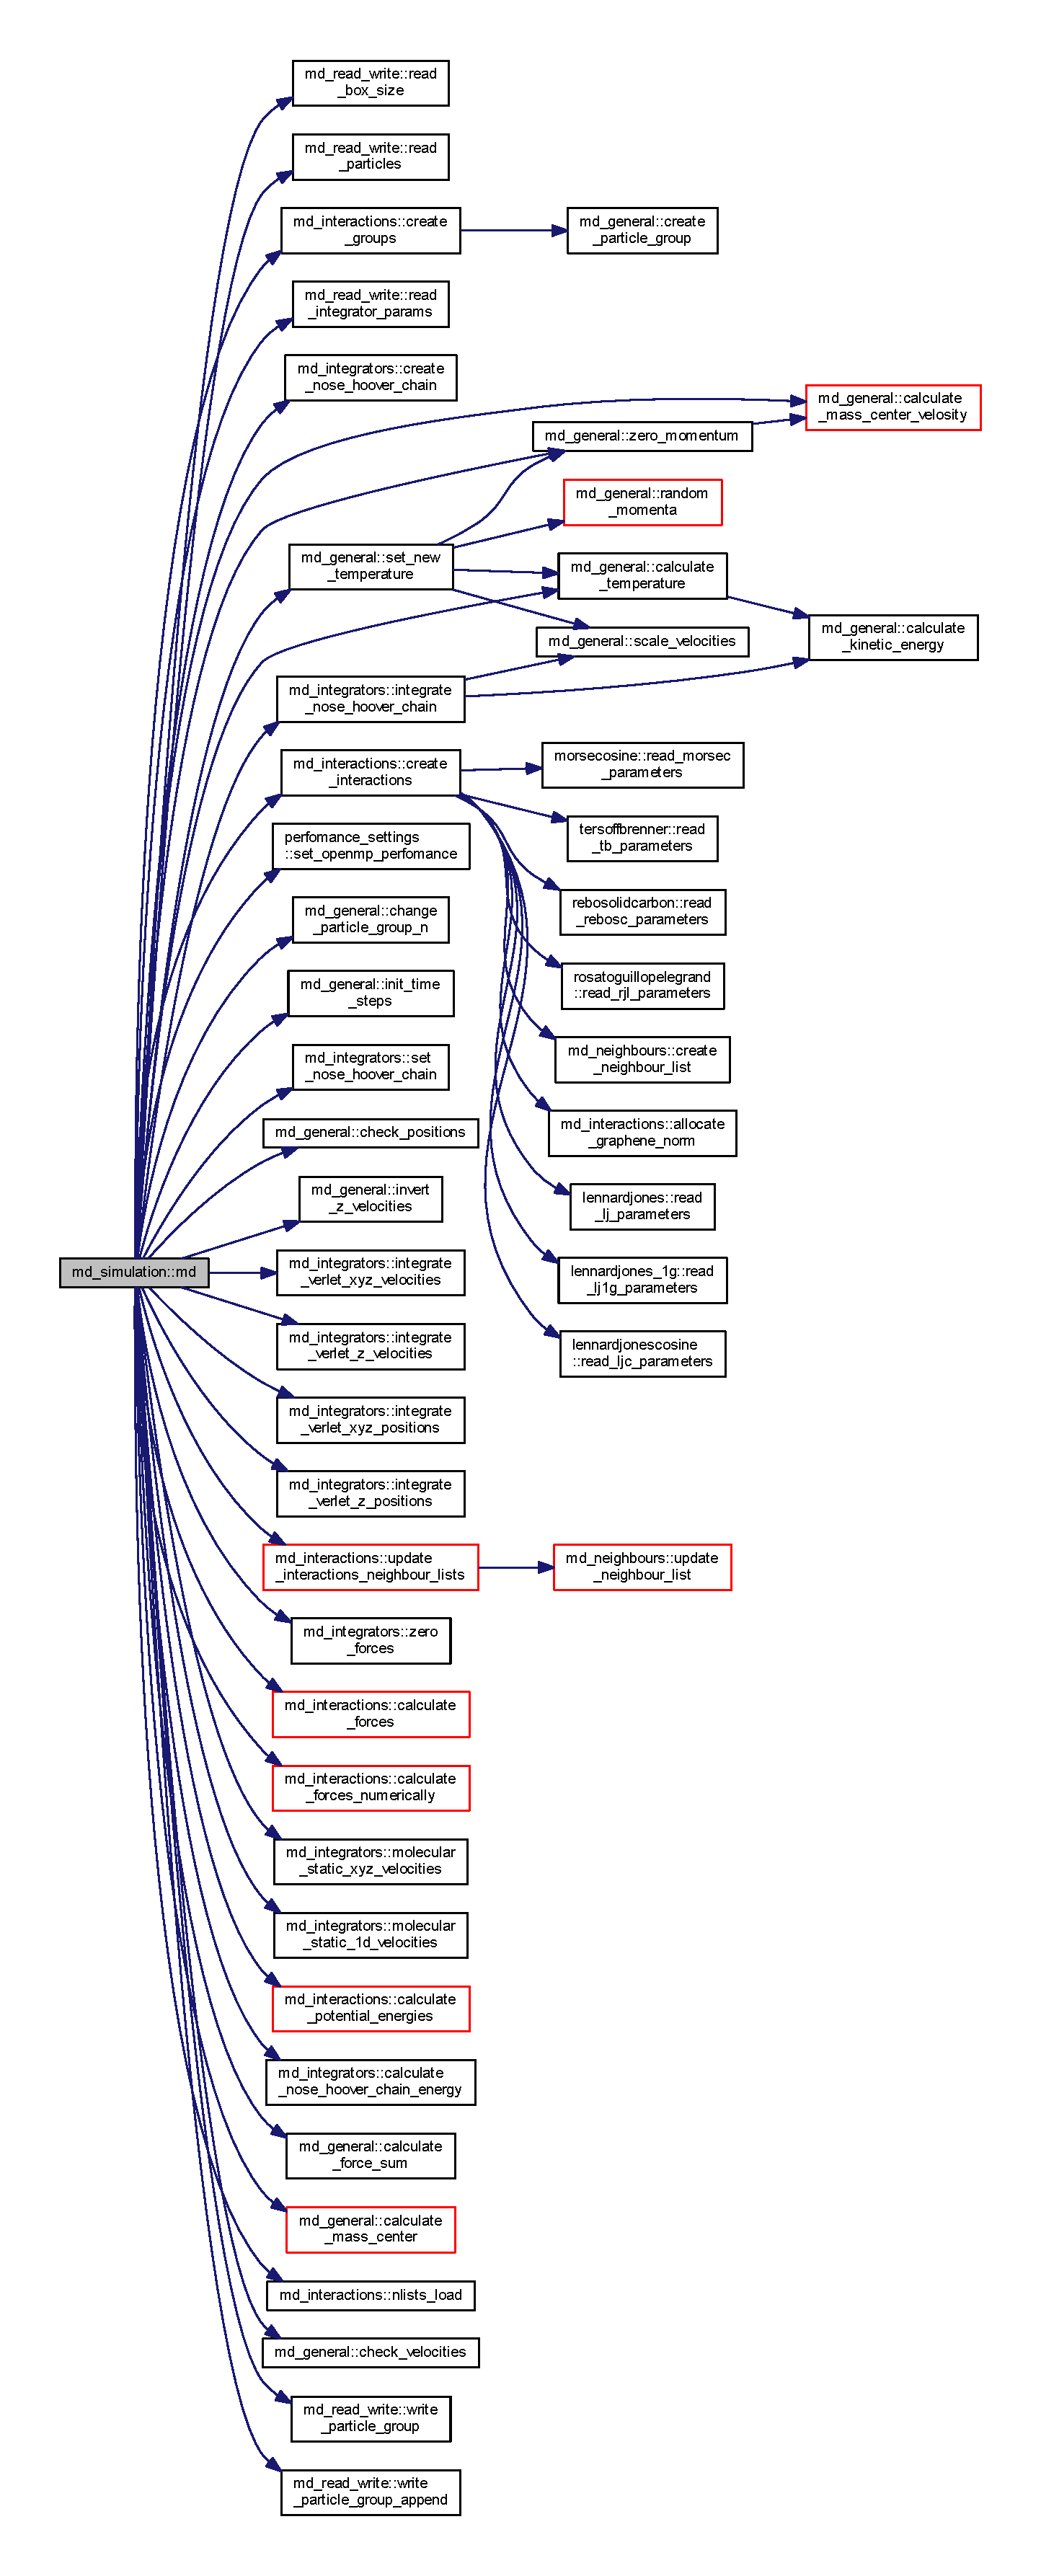
\includegraphics[height=550pt]{namespacemd__simulation_ab2107f3ca598f6a748991632633ee760_cgraph}
\end{center}
\end{figure}

\hypertarget{namespacemorsecosine}{}\section{Модуль morsecosine}
\label{namespacemorsecosine}\index{morsecosine@{morsecosine}}
\subsection*{Типы данных}
\begin{DoxyCompactItemize}
\item 
type \mbox{\hyperlink{structmorsecosine_1_1morsecosine__parameters}{morsecosine\+\_\+parameters}}
\end{DoxyCompactItemize}
\subsection*{Функции/подпрограммы}
\begin{DoxyCompactItemize}
\item 
subroutine \mbox{\hyperlink{namespacemorsecosine_a2d4790950d9c660d18edf6f5dace6031}{read\+\_\+morsec\+\_\+parameters}} (Morse\+Cp, filename)
\item 
subroutine \mbox{\hyperlink{namespacemorsecosine_ab16ff8dd21fbf36d2c97a3905d47702b}{morsec\+\_\+energy}} (energy, nl, Morse\+Cp)
\item 
subroutine \mbox{\hyperlink{namespacemorsecosine_ab762564d1cafd5251e7aac73fbd757db}{morsec\+\_\+forces\+\_\+for\+\_\+graphene}} (atoms, nl, nl\+\_\+nn, Morse\+Cp)
\item 
subroutine \mbox{\hyperlink{namespacemorsecosine_afcca4f80b6e7596c0d7ed68b7346da99}{morsec\+\_\+forces\+\_\+for\+\_\+other\+\_\+atoms}} (atoms, nl, Morse\+Cp)
\end{DoxyCompactItemize}


\subsection{Функции/подпрограммы}
\mbox{\Hypertarget{namespacemorsecosine_ab16ff8dd21fbf36d2c97a3905d47702b}\label{namespacemorsecosine_ab16ff8dd21fbf36d2c97a3905d47702b}} 
\index{morsecosine@{morsecosine}!morsec\+\_\+energy@{morsec\+\_\+energy}}
\index{morsec\+\_\+energy@{morsec\+\_\+energy}!morsecosine@{morsecosine}}
\subsubsection{\texorpdfstring{morsec\+\_\+energy()}{morsec\_energy()}}
{\footnotesize\ttfamily subroutine morsecosine\+::morsec\+\_\+energy (\begin{DoxyParamCaption}\item[{real}]{energy,  }\item[{type(\mbox{\hyperlink{structmd__general_1_1neighbour__list}{neighbour\+\_\+list}})}]{nl,  }\item[{type(\mbox{\hyperlink{structmorsecosine_1_1morsecosine__parameters}{morsecosine\+\_\+parameters}})}]{Morse\+Cp }\end{DoxyParamCaption})}



См. определение в файле Morse\+Cosine.\+f90 строка 27


\begin{DoxyCode}
27     \textcolor{keywordtype}{type}(neighbour\_list):: nl
28     \textcolor{keywordtype}{type}(MorseCosine\_parameters):: MorseCp
29     \textcolor{keywordtype}{integer}:: i,p
30     \textcolor{keywordtype}{real}:: energy,energy\_priv,V1,V2,V3
31     
32     energy = 0.
33     energy\_priv = 0.
34     \textcolor{comment}{!$OMP PARALLEL firstprivate(energy\_priv,i,p,V1,V2,V3)}
35     \textcolor{comment}{!$OMP DO}
36     \textcolor{keywordflow}{do} i=1,nl%N
37         \textcolor{keywordflow}{do} p=1,nl%nnum(i)
38             \textcolor{keywordflow}{if} (nl%moddr(p,i)<morsecp%R2) \textcolor{keywordflow}{then}
39                 v2 = exp(-morsecp%a*(nl%moddr(p,i)-morsecp%r))
40                 v1 = v2**2
41                 v3 = (abs(sum(morsecp%gr\_norm(:,i)*nl%dr(:,p,i)))/nl%moddr(p,i))**morsecp%delt
42                 energy\_priv = energy\_priv+morsecp%d*(v1-2.*v2*v3)*f\_cut(nl%moddr(p,i),morsecp%R1,morsecp%R2
      )
43 \textcolor{keywordflow}{            endif}   
44 \textcolor{keywordflow}{        enddo}
45 \textcolor{keywordflow}{    enddo}
46     \textcolor{comment}{!$OMP END DO}
47     \textcolor{comment}{!$OMP ATOMIC}
48         energy = energy+energy\_priv
49     \textcolor{comment}{!$OMP END PARALLEL}
50     
\end{DoxyCode}
Граф вызовов\+:\nopagebreak
\begin{figure}[H]
\begin{center}
\leavevmode
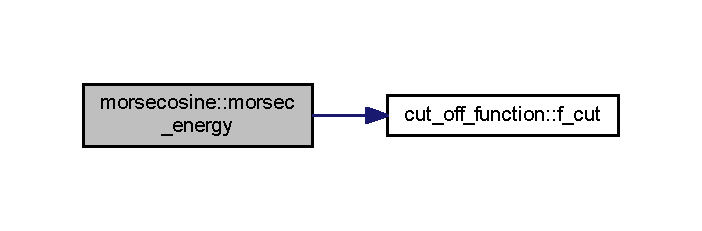
\includegraphics[width=337pt]{namespacemorsecosine_ab16ff8dd21fbf36d2c97a3905d47702b_cgraph}
\end{center}
\end{figure}
\mbox{\Hypertarget{namespacemorsecosine_ab762564d1cafd5251e7aac73fbd757db}\label{namespacemorsecosine_ab762564d1cafd5251e7aac73fbd757db}} 
\index{morsecosine@{morsecosine}!morsec\+\_\+forces\+\_\+for\+\_\+graphene@{morsec\+\_\+forces\+\_\+for\+\_\+graphene}}
\index{morsec\+\_\+forces\+\_\+for\+\_\+graphene@{morsec\+\_\+forces\+\_\+for\+\_\+graphene}!morsecosine@{morsecosine}}
\subsubsection{\texorpdfstring{morsec\+\_\+forces\+\_\+for\+\_\+graphene()}{morsec\_forces\_for\_graphene()}}
{\footnotesize\ttfamily subroutine morsecosine\+::morsec\+\_\+forces\+\_\+for\+\_\+graphene (\begin{DoxyParamCaption}\item[{type(\mbox{\hyperlink{structmd__general_1_1particles}{particles}})}]{atoms,  }\item[{type(\mbox{\hyperlink{structmd__general_1_1neighbour__list}{neighbour\+\_\+list}})}]{nl,  }\item[{type(\mbox{\hyperlink{structmd__general_1_1neighbour__list}{neighbour\+\_\+list}})}]{nl\+\_\+nn,  }\item[{type(\mbox{\hyperlink{structmorsecosine_1_1morsecosine__parameters}{morsecosine\+\_\+parameters}})}]{Morse\+Cp }\end{DoxyParamCaption})}



См. определение в файле Morse\+Cosine.\+f90 строка 54


\begin{DoxyCode}
54     \textcolor{keywordtype}{type}(particles)::   atoms
55     \textcolor{keywordtype}{type}(neighbour\_list):: nl,nl\_nn
56     \textcolor{keywordtype}{type}(MorseCosine\_parameters):: MorseCp
57     \textcolor{keywordtype}{integer}:: i,p,q,l1,l2,l3,j,k,nnum\_nn
58     \textcolor{keywordtype}{real}:: drj12(3),drj31(3),drj23(3),V1,V2,V3,f\_c,df\_c
59     
60     \textcolor{keywordflow}{if} (nl%N/=nl\_nn%N .and. nl%N/=0) then; \textcolor{keyword}{write}(*,*) \textcolor{stringliteral}{'error: nl%N/=nl\_nn%N'},nl%N,nl\_nn%N; stop;\textcolor{keywordflow}{ endif}
61     nnum\_nn = 3
62     \textcolor{keywordflow}{if} (morsecp%simplified) then; nnum\_nn = 0; morsecp%gr\_norm = 0.; morsecp%gr\_norm(3,:) = 1.; endif\textcolor{comment}{
      !optimize}
63     
64     \textcolor{comment}{!$OMP PARALLEL firstprivate(i,p,q,l1,l2,l3,j,k,drj12,drj31,drj23,V1,V2,V3,f\_c,df\_c)}
65     \textcolor{comment}{!$OMP DO}
66     \textcolor{keywordflow}{do} i=1,nl%N
67         \textcolor{keywordflow}{do} p=1,nl%nnum(i)
68             \textcolor{keywordflow}{if} (nl%moddr(p,i)<morsecp%R2) \textcolor{keywordflow}{then}
69                 v2 = exp(-morsecp%a*(nl%moddr(p,i)-morsecp%r))
70                 v1 = v2**2
71                 v3 = (abs(sum(morsecp%gr\_norm(:,i)*nl%dr(:,p,i)))/nl%moddr(p,i))**morsecp%delt
72                 f\_c = f\_cut(nl%moddr(p,i),morsecp%R1,morsecp%R2)
73                 df\_c = df\_cut(nl%moddr(p,i),morsecp%R1,morsecp%R2)
74                 atoms%forces(:,nl%particle\_index(i)) = atoms%forces(:,nl%particle\_index(i))-morsecp%d*&
75                 ((2.*(morsecp%a*v1-(morsecp%a+morsecp%delt/nl%moddr(p,i))*v2*v3)/nl%moddr(p,i)*f\_c-(v1-2.*
      v2*v3)*df\_c)*nl%dr(:,p,i)+&
76                 (2.*morsecp%delt*v2*v3/sum(morsecp%gr\_norm(:,i)*nl%dr(:,p,i))*f\_c)*morsecp%gr\_norm(:,i))
77 \textcolor{keywordflow}{            endif}
78 \textcolor{keywordflow}{        enddo}
79 \textcolor{keywordflow}{    enddo}
80     \textcolor{comment}{!$OMP END DO}
81     \textcolor{comment}{!$OMP DO}
82     \textcolor{keywordflow}{do} i=1,nl%N
83         \textcolor{keywordflow}{do} q=1,nnum\_nn
84             j = nl\_nn%nlist(q,i)
85             \textcolor{keywordflow}{do} l1=1,nnum\_nn
86                 \textcolor{keywordflow}{if} (nl\_nn%nlist(l1,j)==i) \textcolor{keywordflow}{exit}
87 \textcolor{keywordflow}{            enddo}
88             \textcolor{keywordflow}{if}(l1>3) then; \textcolor{keyword}{write}(*,*) \textcolor{stringliteral}{'l1>3'}; stop;\textcolor{keywordflow}{ endif}
89             l2 = mod(l1,3)+1
90             l3 = mod(l1+1,3)+1
91             drj12 = nl\_nn%dr(:,l2,j)-nl\_nn%dr(:,l1,j)
92             drj31 = nl\_nn%dr(:,l1,j)-nl\_nn%dr(:,l3,j)
93             drj23 = nl\_nn%dr(:,l3,j)-nl\_nn%dr(:,l2,j)
94             \textcolor{keywordflow}{do} p=1,nl%nnum(j)
95                 \textcolor{keywordflow}{if} (nl%moddr(p,j)<morsecp%R2) \textcolor{keywordflow}{then}
96                     v2 = exp(-morsecp%a*(nl%moddr(p,j)-morsecp%r))
97                     v1 = v2**2
98                     v3 = (abs(sum(morsecp%gr\_norm(:,j)*nl%dr(:,p,j)))/nl%moddr(p,j))**morsecp%delt
99                     f\_c = f\_cut(nl%moddr(p,j),morsecp%R1,morsecp%R2)
100                     atoms%forces(:,nl%particle\_index(i)) = atoms%forces(:,nl%particle\_index(i))&
101                     -2.*morsecp%d*morsecp%delt*v2*v3*f\_c/(sum(drj12**2)*sum(drj31**2)-sum(drj12*drj31)**2)/
      sum(morsecp%gr\_norm(:,j)*nl%dr(:,p,j))*&
102                     morsecp%gr\_norm(:,j)*sum(nl%dr(:,p,j)*(drj12*sum(drj23*drj31)-drj31*sum(drj23*drj12)))
103 \textcolor{keywordflow}{                endif}
104 \textcolor{keywordflow}{            enddo}
105 \textcolor{keywordflow}{        enddo}
106 \textcolor{keywordflow}{    enddo}
107     \textcolor{comment}{!$OMP END DO}
108     \textcolor{comment}{!$OMP END PARALLEL}
109     
\end{DoxyCode}
Граф вызовов\+:\nopagebreak
\begin{figure}[H]
\begin{center}
\leavevmode
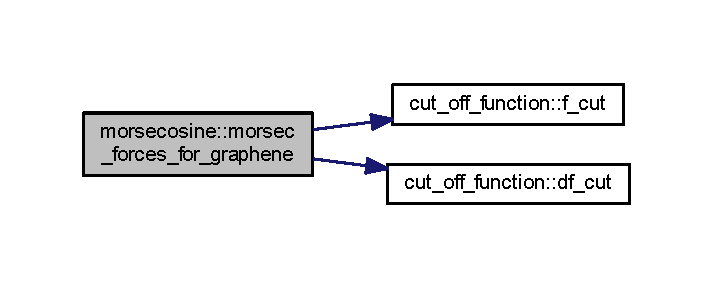
\includegraphics[width=342pt]{namespacemorsecosine_ab762564d1cafd5251e7aac73fbd757db_cgraph}
\end{center}
\end{figure}
\mbox{\Hypertarget{namespacemorsecosine_afcca4f80b6e7596c0d7ed68b7346da99}\label{namespacemorsecosine_afcca4f80b6e7596c0d7ed68b7346da99}} 
\index{morsecosine@{morsecosine}!morsec\+\_\+forces\+\_\+for\+\_\+other\+\_\+atoms@{morsec\+\_\+forces\+\_\+for\+\_\+other\+\_\+atoms}}
\index{morsec\+\_\+forces\+\_\+for\+\_\+other\+\_\+atoms@{morsec\+\_\+forces\+\_\+for\+\_\+other\+\_\+atoms}!morsecosine@{morsecosine}}
\subsubsection{\texorpdfstring{morsec\+\_\+forces\+\_\+for\+\_\+other\+\_\+atoms()}{morsec\_forces\_for\_other\_atoms()}}
{\footnotesize\ttfamily subroutine morsecosine\+::morsec\+\_\+forces\+\_\+for\+\_\+other\+\_\+atoms (\begin{DoxyParamCaption}\item[{type(\mbox{\hyperlink{structmd__general_1_1particles}{particles}})}]{atoms,  }\item[{type(\mbox{\hyperlink{structmd__general_1_1neighbour__list}{neighbour\+\_\+list}})}]{nl,  }\item[{type(\mbox{\hyperlink{structmorsecosine_1_1morsecosine__parameters}{morsecosine\+\_\+parameters}})}]{Morse\+Cp }\end{DoxyParamCaption})}



См. определение в файле Morse\+Cosine.\+f90 строка 113


\begin{DoxyCode}
113     \textcolor{keywordtype}{type}(particles)::   atoms
114     \textcolor{keywordtype}{type}(neighbour\_list):: nl
115     \textcolor{keywordtype}{type}(MorseCosine\_parameters):: MorseCp
116     \textcolor{keywordtype}{integer}:: i,p
117     \textcolor{keywordtype}{real}:: gr\_n(3),V1,V2,V3,f\_c,df\_c
118     
119     \textcolor{comment}{!$OMP PARALLEL firstprivate(i,p,gr\_n,V1,V2,V3,f\_c,df\_c)}
120     \textcolor{comment}{!$OMP DO}
121     \textcolor{keywordflow}{do} i=1,nl%N
122         \textcolor{keywordflow}{do} p=1,nl%nnum(i)
123             \textcolor{keywordflow}{if} (nl%moddr(p,i)<morsecp%R2) \textcolor{keywordflow}{then}
124                 gr\_n = morsecp%gr\_norm(:,nl%nlist(p,i))
125                 v2 = exp(-morsecp%a*(nl%moddr(p,i)-morsecp%r))
126                 v1 = v2**2
127                 v3 = (abs(sum(gr\_n*nl%dr(:,p,i)))/(sqrt(sum(gr\_n**2))*nl%moddr(p,i)))**morsecp%delt
128                 f\_c = f\_cut(nl%moddr(p,i),morsecp%R1,morsecp%R2)
129                 df\_c = df\_cut(nl%moddr(p,i),morsecp%R1,morsecp%R2)
130                 atoms%forces(:,nl%particle\_index(i)) = atoms%forces(:,nl%particle\_index(i))-morsecp%d*&
131                 ((2.*(morsecp%a*v1-(morsecp%a+morsecp%delt/nl%moddr(p,i))*v2*v3)/nl%moddr(p,i)*f\_c-(v1-2.*
      v2*v3)*df\_c)*nl%dr(:,p,i)+&
132                 (2.*morsecp%delt*v2*v3/sum(gr\_n*nl%dr(:,p,i))*f\_c)*gr\_n)
133 \textcolor{keywordflow}{            endif}
134 \textcolor{keywordflow}{        enddo}
135 \textcolor{keywordflow}{    enddo}
136     \textcolor{comment}{!$OMP END DO }
137     \textcolor{comment}{!$OMP END PARALLEL}
138     
\end{DoxyCode}
Граф вызовов\+:\nopagebreak
\begin{figure}[H]
\begin{center}
\leavevmode
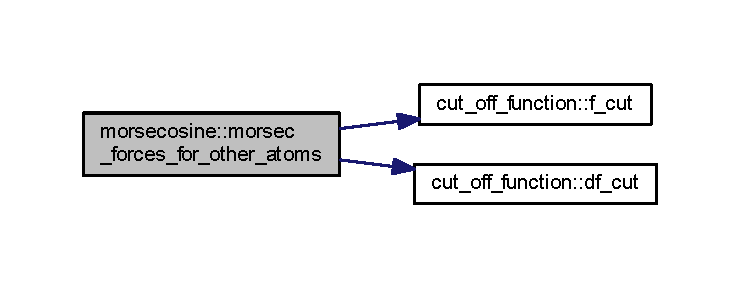
\includegraphics[width=350pt]{namespacemorsecosine_afcca4f80b6e7596c0d7ed68b7346da99_cgraph}
\end{center}
\end{figure}
\mbox{\Hypertarget{namespacemorsecosine_a2d4790950d9c660d18edf6f5dace6031}\label{namespacemorsecosine_a2d4790950d9c660d18edf6f5dace6031}} 
\index{morsecosine@{morsecosine}!read\+\_\+morsec\+\_\+parameters@{read\+\_\+morsec\+\_\+parameters}}
\index{read\+\_\+morsec\+\_\+parameters@{read\+\_\+morsec\+\_\+parameters}!morsecosine@{morsecosine}}
\subsubsection{\texorpdfstring{read\+\_\+morsec\+\_\+parameters()}{read\_morsec\_parameters()}}
{\footnotesize\ttfamily subroutine morsecosine\+::read\+\_\+morsec\+\_\+parameters (\begin{DoxyParamCaption}\item[{type(\mbox{\hyperlink{structmorsecosine_1_1morsecosine__parameters}{morsecosine\+\_\+parameters}})}]{Morse\+Cp,  }\item[{character($\ast$)}]{filename }\end{DoxyParamCaption})}



См. определение в файле Morse\+Cosine.\+f90 строка 15


\begin{DoxyCode}
15     \textcolor{keywordtype}{type}(MorseCosine\_parameters):: MorseCp
16     \textcolor{keywordtype}{character(*)}::  filename
17     
18     \textcolor{keyword}{open}(1,file=filename)
19     \textcolor{keyword}{read}(1,*) morsecp%d,morsecp%r,morsecp%a,morsecp%delt
20     \textcolor{keyword}{read}(1,*) morsecp%R1,morsecp%R2
21     \textcolor{keyword}{read}(1,*) morsecp%simplified
22     \textcolor{keyword}{close}(1)
23     
\end{DoxyCode}

\hypertarget{namespaceperfomance__settings}{}\section{Модуль perfomance\+\_\+settings}
\label{namespaceperfomance__settings}\index{perfomance\+\_\+settings@{perfomance\+\_\+settings}}


Модуль настройки Open\+MP параллелизма.  


\subsection*{Функции/подпрограммы}
\begin{DoxyCompactItemize}
\item 
subroutine \mbox{\hyperlink{namespaceperfomance__settings_a50a101c3721ccc0da3b5867807ea6c70}{set\+\_\+openmp\+\_\+perfomance}} (num\+\_\+of\+\_\+omp\+\_\+treads, N)
\begin{DoxyCompactList}\small\item\em Настраивает количество Open\+MP потоков и omp\+\_\+chunk\+\_\+size. \end{DoxyCompactList}\end{DoxyCompactItemize}
\subsection*{Переменные}
\begin{DoxyCompactItemize}
\item 
integer \mbox{\hyperlink{namespaceperfomance__settings_a1632739c07471b87731fe9e33f69fcae}{omp\+\_\+chunk\+\_\+size}}
\begin{DoxyCompactList}\small\item\em Массивы данных будут разбиваться на части длины omp\+\_\+chunk\+\_\+size при использовании omp parallel for schedule(dynamic ,omp\+\_\+chunk\+\_\+size) \end{DoxyCompactList}\end{DoxyCompactItemize}


\subsection{Подробное описание}
Модуль настройки Open\+MP параллелизма. 

\begin{DoxyWarning}{Предупреждения}
omp\+\_\+chunk\+\_\+size пока нигде не используется. 
\end{DoxyWarning}


\subsection{Функции/подпрограммы}
\mbox{\Hypertarget{namespaceperfomance__settings_a50a101c3721ccc0da3b5867807ea6c70}\label{namespaceperfomance__settings_a50a101c3721ccc0da3b5867807ea6c70}} 
\index{perfomance\+\_\+settings@{perfomance\+\_\+settings}!set\+\_\+openmp\+\_\+perfomance@{set\+\_\+openmp\+\_\+perfomance}}
\index{set\+\_\+openmp\+\_\+perfomance@{set\+\_\+openmp\+\_\+perfomance}!perfomance\+\_\+settings@{perfomance\+\_\+settings}}
\subsubsection{\texorpdfstring{set\+\_\+openmp\+\_\+perfomance()}{set\_openmp\_perfomance()}}
{\footnotesize\ttfamily subroutine perfomance\+\_\+settings\+::set\+\_\+openmp\+\_\+perfomance (\begin{DoxyParamCaption}\item[{integer}]{num\+\_\+of\+\_\+omp\+\_\+treads,  }\item[{integer}]{N }\end{DoxyParamCaption})}



Настраивает количество Open\+MP потоков и omp\+\_\+chunk\+\_\+size. 


\begin{DoxyParams}{Аргументы}
{\em num\+\_\+of\+\_\+omp\+\_\+treads} & Количество Open\+MP потоков\\
\hline
{\em n} & Количество частиц в моделируемой системе \\
\hline
\end{DoxyParams}


См. определение в файле perfomance\+\_\+settings.\+f90 строка 14


\begin{DoxyCode}
14     \textcolor{keywordtype}{integer}:: chunks\_per\_thread
15     \textcolor{keywordtype}{integer}:: num\_of\_omp\_treads
16     \textcolor{keywordtype}{integer}:: N
17     
18     \textcolor{keyword}{call }omp\_set\_num\_threads(num\_of\_omp\_treads)
19     \textcolor{comment}{!call omp\_thread\_limit(num\_of\_omp\_treads)}
20     
21     chunks\_per\_thread = 8
22     omp\_chunk\_size = int(\textcolor{keywordtype}{real}(N)/chunks\_per\_thread/num\_of\_omp\_treads)
23     \textcolor{keywordflow}{if}(omp\_chunk\_size==0) omp\_chunk\_size = 1
24     
\end{DoxyCode}


\subsection{Переменные}
\mbox{\Hypertarget{namespaceperfomance__settings_a1632739c07471b87731fe9e33f69fcae}\label{namespaceperfomance__settings_a1632739c07471b87731fe9e33f69fcae}} 
\index{perfomance\+\_\+settings@{perfomance\+\_\+settings}!omp\+\_\+chunk\+\_\+size@{omp\+\_\+chunk\+\_\+size}}
\index{omp\+\_\+chunk\+\_\+size@{omp\+\_\+chunk\+\_\+size}!perfomance\+\_\+settings@{perfomance\+\_\+settings}}
\subsubsection{\texorpdfstring{omp\+\_\+chunk\+\_\+size}{omp\_chunk\_size}}
{\footnotesize\ttfamily integer perfomance\+\_\+settings\+::omp\+\_\+chunk\+\_\+size}



Массивы данных будут разбиваться на части длины omp\+\_\+chunk\+\_\+size при использовании omp parallel for schedule(dynamic ,omp\+\_\+chunk\+\_\+size) 



См. определение в файле perfomance\+\_\+settings.\+f90 строка 8


\begin{DoxyCode}
8 \textcolor{keywordtype}{integer}:: omp\_chunk\_size
\end{DoxyCode}

\hypertarget{namespacerebosolidcarbon}{}\section{Модуль rebosolidcarbon}
\label{namespacerebosolidcarbon}\index{rebosolidcarbon@{rebosolidcarbon}}
\subsection*{Типы данных}
\begin{DoxyCompactItemize}
\item 
type \mbox{\hyperlink{structrebosolidcarbon_1_1rebosc__parameters}{rebosc\+\_\+parameters}}
\end{DoxyCompactItemize}
\subsection*{Функции/подпрограммы}
\begin{DoxyCompactItemize}
\item 
subroutine \mbox{\hyperlink{namespacerebosolidcarbon_ac08d3d8f908fa0578d4565b200e96df0}{read\+\_\+rebosc\+\_\+parameters}} (R\+E\+B\+Oscp, filename)
\item 
subroutine \mbox{\hyperlink{namespacerebosolidcarbon_a300f2042f4b21284cfa42c0e4de3f0a8}{rebosc\+\_\+energy}} (energy, nl, R\+E\+B\+Oscp)
\end{DoxyCompactItemize}


\subsection{Функции/подпрограммы}
\mbox{\Hypertarget{namespacerebosolidcarbon_ac08d3d8f908fa0578d4565b200e96df0}\label{namespacerebosolidcarbon_ac08d3d8f908fa0578d4565b200e96df0}} 
\index{rebosolidcarbon@{rebosolidcarbon}!read\+\_\+rebosc\+\_\+parameters@{read\+\_\+rebosc\+\_\+parameters}}
\index{read\+\_\+rebosc\+\_\+parameters@{read\+\_\+rebosc\+\_\+parameters}!rebosolidcarbon@{rebosolidcarbon}}
\subsubsection{\texorpdfstring{read\+\_\+rebosc\+\_\+parameters()}{read\_rebosc\_parameters()}}
{\footnotesize\ttfamily subroutine rebosolidcarbon\+::read\+\_\+rebosc\+\_\+parameters (\begin{DoxyParamCaption}\item[{type(\mbox{\hyperlink{structrebosolidcarbon_1_1rebosc__parameters}{rebosc\+\_\+parameters}})}]{R\+E\+B\+Oscp,  }\item[{character($\ast$)}]{filename }\end{DoxyParamCaption})}



См. определение в файле R\+E\+B\+Osolidcarbon.\+f90 строка 13


\begin{DoxyCode}
13     \textcolor{keywordtype}{type}(REBOsc\_parameters):: REBOscp
14     \textcolor{keywordtype}{character(*)}::  filename
15 
16     \textcolor{keyword}{open}(1,file=filename)
17     \textcolor{keyword}{read}(1,*) reboscp%A,reboscp%Q,reboscp%alpha
18     \textcolor{keyword}{read}(1,*) reboscp%B
19     \textcolor{keyword}{read}(1,*) reboscp%beta
20     \textcolor{keyword}{read}(1,*) reboscp%T
21     \textcolor{keyword}{read}(1,*) reboscp%g
22     \textcolor{keyword}{read}(1,*) reboscp%R1,reboscp%R2
23     \textcolor{keyword}{close}(1)
24     
\end{DoxyCode}
\mbox{\Hypertarget{namespacerebosolidcarbon_a300f2042f4b21284cfa42c0e4de3f0a8}\label{namespacerebosolidcarbon_a300f2042f4b21284cfa42c0e4de3f0a8}} 
\index{rebosolidcarbon@{rebosolidcarbon}!rebosc\+\_\+energy@{rebosc\+\_\+energy}}
\index{rebosc\+\_\+energy@{rebosc\+\_\+energy}!rebosolidcarbon@{rebosolidcarbon}}
\subsubsection{\texorpdfstring{rebosc\+\_\+energy()}{rebosc\_energy()}}
{\footnotesize\ttfamily subroutine rebosolidcarbon\+::rebosc\+\_\+energy (\begin{DoxyParamCaption}\item[{real}]{energy,  }\item[{type(\mbox{\hyperlink{structmd__general_1_1neighbour__list}{neighbour\+\_\+list}})}]{nl,  }\item[{type(\mbox{\hyperlink{structrebosolidcarbon_1_1rebosc__parameters}{rebosc\+\_\+parameters}})}]{R\+E\+B\+Oscp }\end{DoxyParamCaption})}



См. определение в файле R\+E\+B\+Osolidcarbon.\+f90 строка 28


\begin{DoxyCode}
28     \textcolor{keywordtype}{type}(neighbour\_list):: nl
29     \textcolor{keywordtype}{type}(REBOsc\_parameters):: REBOscp
30     \textcolor{keywordtype}{integer}:: i,p,q,l,j
31     \textcolor{keywordtype}{real}:: energy,energy\_priv,bsp(nl%neighb\_num\_max,nl%N),bdh(nl%neighb\_num\_max,nl%N),aa,ab,ac,bc,cosine
32     
33     energy = 0.
34     energy\_priv = 0.
35     \textcolor{comment}{!$OMP PARALLEL firstprivate(energy\_priv,i,p,q,l,j,aa,ab,ac,bc,cosine)}
36     \textcolor{comment}{!$OMP DO}
37     \textcolor{keywordflow}{do} i=1,nl%N
38         bsp(:,i) = 0. \textcolor{comment}{!not very optimal but hides a bug(?) in numerical forse calc in parallel}
39         bdh(:,i) = 0.
40         \textcolor{keywordflow}{do} p=1,nl%nnum(i)
41             \textcolor{comment}{!bsp(p,i) = 0.}
42             \textcolor{comment}{!bdh(p,i) = 0.}
43             \textcolor{keywordflow}{if} (nl%moddr(p,i)<reboscp%R2) \textcolor{keywordflow}{then}
44                 j = nl%nlist(p,i)
45                 \textcolor{keywordflow}{do} q=1,nl%nnum(i)
46                     \textcolor{keywordflow}{if}(p/=q .and. nl%moddr(q,i)<reboscp%R2) \textcolor{keywordflow}{then}
47                         cosine = sum(nl%dr(:,p,i)*nl%dr(:,q,i))/(nl%moddr(p,i)*nl%moddr(q,i))
48                         bsp(p,i) = bsp(p,i)+f\_cut(nl%moddr(q,i),reboscp%R1,reboscp%R2)*(reboscp%g(1)+
      reboscp%g(2)*cosine+&
49                         reboscp%g(3)*cosine**2+reboscp%g(4)*cosine**3+reboscp%g(5)*cosine**4+reboscp%g(6)*
      cosine**5)
50                         \textcolor{keywordflow}{do} l=1,nl%nnum(j) \textcolor{comment}{!mb if j>i?}
51                             \textcolor{keywordflow}{if}(nl%nlist(l,j)/=i .and. nl%moddr(l,j)<reboscp%R2) \textcolor{keywordflow}{then}
52                                 aa = nl%moddr(p,i)**2
53                                 ab = sum(nl%dr(:,p,i)*nl%dr(:,q,i))
54                                 ac = sum(nl%dr(:,p,i)*nl%dr(:,l,j))
55                                 bc = sum(nl%dr(:,q,i)*nl%dr(:,l,j))
56                                 bdh(p,i) = bdh(p,i)+f\_cut(nl%moddr(q,i),reboscp%R1,reboscp%R2)*f\_cut(nl
      %moddr(l,j),reboscp%R1,reboscp%R2)*&
57                                 (1.-(aa*bc-ab*ac)**2/(aa*nl%moddr(q,i)**2-ab**2)/(aa*nl%moddr(l,j)**2-ac**2
      ))
58 \textcolor{keywordflow}{                            endif}
59 \textcolor{keywordflow}{                        enddo}
60 \textcolor{keywordflow}{                    endif}
61 \textcolor{keywordflow}{                enddo}
62                 bsp(p,i) = (1.+bsp(p,i))**(-0.5)
63                 bdh(p,i) = reboscp%T*bdh(p,i)
64 \textcolor{keywordflow}{            endif}
65 \textcolor{keywordflow}{        enddo}
66 \textcolor{keywordflow}{    enddo}
67     \textcolor{comment}{!$OMP END DO}
68     \textcolor{comment}{!$OMP DO}
69     \textcolor{keywordflow}{do} i=1,nl%N
70         \textcolor{keywordflow}{do} p=1,nl%nnum(i)
71             \textcolor{keywordflow}{if} (nl%moddr(p,i)<reboscp%R2) \textcolor{keywordflow}{then}
72                 j = nl%nlist(p,i)
73                 \textcolor{keywordflow}{if} (j>i) \textcolor{keywordflow}{then}
74                     \textcolor{keywordflow}{do} q=1,nl%nnum(j)
75                         \textcolor{keywordflow}{if}(nl%nlist(q,j)==i) \textcolor{keywordflow}{exit}
76 \textcolor{keywordflow}{                    enddo}
77                     energy\_priv = energy\_priv+f\_cut(nl%moddr(p,i),reboscp%R1,reboscp%R2)*&
78                     ((1+reboscp%Q/nl%moddr(p,i))*reboscp%A*exp(-reboscp%alpha*nl%moddr(p,i))-&
79                     ((bsp(p,i)+bsp(q,j))/2+bdh(p,i))*&
80                     (reboscp%B(1)*exp(-reboscp%beta(1)*nl%moddr(p,i))+&
81                     reboscp%B(2)*exp(-reboscp%beta(2)*nl%moddr(p,i))+&
82                     reboscp%B(3)*exp(-reboscp%beta(3)*nl%moddr(p,i))))
83 \textcolor{keywordflow}{                endif}
84 \textcolor{keywordflow}{            endif}
85 \textcolor{keywordflow}{        enddo}
86 \textcolor{keywordflow}{    enddo}
87     \textcolor{comment}{!$OMP END DO}
88     \textcolor{comment}{!$OMP ATOMIC}
89         energy = energy+energy\_priv
90     \textcolor{comment}{!$OMP END PARALLEL}
91     
\end{DoxyCode}
Граф вызовов\+:\nopagebreak
\begin{figure}[H]
\begin{center}
\leavevmode
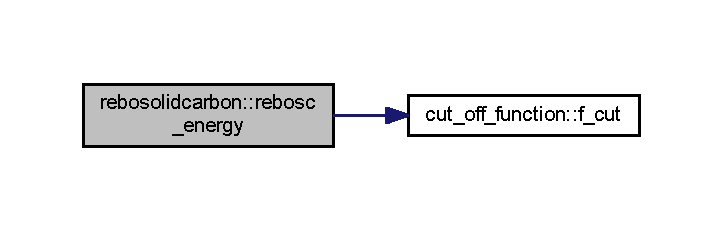
\includegraphics[width=347pt]{namespacerebosolidcarbon_a300f2042f4b21284cfa42c0e4de3f0a8_cgraph}
\end{center}
\end{figure}

\hypertarget{namespacerosatoguillopelegrand}{}\section{Модуль rosatoguillopelegrand}
\label{namespacerosatoguillopelegrand}\index{rosatoguillopelegrand@{rosatoguillopelegrand}}
\subsection*{Типы данных}
\begin{DoxyCompactItemize}
\item 
type \mbox{\hyperlink{structrosatoguillopelegrand_1_1rosatoguillopelegrand__parameters}{rosatoguillopelegrand\+\_\+parameters}}
\end{DoxyCompactItemize}
\subsection*{Функции/подпрограммы}
\begin{DoxyCompactItemize}
\item 
subroutine \mbox{\hyperlink{namespacerosatoguillopelegrand_ac5fa55316f7b8e860b3131c6f95c10ae}{read\+\_\+rjl\+\_\+parameters}} (R\+J\+Lp, filename)
\item 
subroutine \mbox{\hyperlink{namespacerosatoguillopelegrand_a06b6c23e50e301e053ed9ccb60e1ca34}{rjl\+\_\+energy}} (energy, nl, R\+J\+Lp)
\item 
subroutine \mbox{\hyperlink{namespacerosatoguillopelegrand_a3744fc3d1e6df3ca288ddc43df483ca0}{rjl\+\_\+forces}} (atoms, nl, R\+J\+Lp)
\end{DoxyCompactItemize}


\subsection{Функции/подпрограммы}
\mbox{\Hypertarget{namespacerosatoguillopelegrand_ac5fa55316f7b8e860b3131c6f95c10ae}\label{namespacerosatoguillopelegrand_ac5fa55316f7b8e860b3131c6f95c10ae}} 
\index{rosatoguillopelegrand@{rosatoguillopelegrand}!read\+\_\+rjl\+\_\+parameters@{read\+\_\+rjl\+\_\+parameters}}
\index{read\+\_\+rjl\+\_\+parameters@{read\+\_\+rjl\+\_\+parameters}!rosatoguillopelegrand@{rosatoguillopelegrand}}
\subsubsection{\texorpdfstring{read\+\_\+rjl\+\_\+parameters()}{read\_rjl\_parameters()}}
{\footnotesize\ttfamily subroutine rosatoguillopelegrand\+::read\+\_\+rjl\+\_\+parameters (\begin{DoxyParamCaption}\item[{type(\mbox{\hyperlink{structrosatoguillopelegrand_1_1rosatoguillopelegrand__parameters}{rosatoguillopelegrand\+\_\+parameters}})}]{R\+J\+Lp,  }\item[{character($\ast$)}]{filename }\end{DoxyParamCaption})}



См. определение в файле Rosato\+Guillope\+Legrand.\+f90 строка 13


\begin{DoxyCode}
13     \textcolor{keywordtype}{type}(RosatoGuillopeLegrand\_parameters):: RJLp
14     \textcolor{keywordtype}{character(*)}::  filename
15     
16     \textcolor{keyword}{open}(1,file=filename)
17     \textcolor{keyword}{read}(1,*) rjlp%A0,rjlp%xi,rjlp%p,rjlp%q,rjlp%r0
18     \textcolor{keyword}{read}(1,*) rjlp%R1,rjlp%R2
19     \textcolor{keyword}{close}(1)
20     
\end{DoxyCode}
\mbox{\Hypertarget{namespacerosatoguillopelegrand_a06b6c23e50e301e053ed9ccb60e1ca34}\label{namespacerosatoguillopelegrand_a06b6c23e50e301e053ed9ccb60e1ca34}} 
\index{rosatoguillopelegrand@{rosatoguillopelegrand}!rjl\+\_\+energy@{rjl\+\_\+energy}}
\index{rjl\+\_\+energy@{rjl\+\_\+energy}!rosatoguillopelegrand@{rosatoguillopelegrand}}
\subsubsection{\texorpdfstring{rjl\+\_\+energy()}{rjl\_energy()}}
{\footnotesize\ttfamily subroutine rosatoguillopelegrand\+::rjl\+\_\+energy (\begin{DoxyParamCaption}\item[{real}]{energy,  }\item[{type(\mbox{\hyperlink{structmd__general_1_1neighbour__list}{neighbour\+\_\+list}})}]{nl,  }\item[{type(\mbox{\hyperlink{structrosatoguillopelegrand_1_1rosatoguillopelegrand__parameters}{rosatoguillopelegrand\+\_\+parameters}})}]{R\+J\+Lp }\end{DoxyParamCaption})}



См. определение в файле Rosato\+Guillope\+Legrand.\+f90 строка 24


\begin{DoxyCode}
24     \textcolor{keywordtype}{type}(RosatoGuillopeLegrand\_parameters):: RJLp
25     \textcolor{keywordtype}{type}(neighbour\_list):: nl
26     \textcolor{keywordtype}{integer}:: i,p
27     \textcolor{keywordtype}{real}:: energy,energy\_priv,Eb2,Er
28     
29     energy = 0.
30     energy\_priv = 0.
31     \textcolor{comment}{!$OMP PARALLEL firstprivate(energy\_priv,i,p,Eb2,Er)}
32     \textcolor{comment}{!$OMP DO}
33     \textcolor{keywordflow}{do} i=1,nl%N
34         eb2 = 0.
35         er = 0.
36         \textcolor{keywordflow}{do} p=1,nl%nnum(i)
37             \textcolor{keywordflow}{if}( nl%moddr(p,i)<=rjlp%R2 ) \textcolor{keywordflow}{then}
38                 eb2 = eb2+exp(-2.*rjlp%q*(nl%moddr(p,i)/rjlp%r0-1.))*f\_cut(nl%moddr(p,i),rjlp%R1,rjlp%R2)
39                 er = er+exp(-rjlp%p*(nl%moddr(p,i)/rjlp%r0-1.))*f\_cut(nl%moddr(p,i),rjlp%R1,rjlp%R2)
40 \textcolor{keywordflow}{            endif}
41 \textcolor{keywordflow}{        enddo}
42         energy\_priv = energy\_priv+rjlp%A0*er-rjlp%xi*sqrt(eb2)
43 \textcolor{keywordflow}{    enddo}
44     \textcolor{comment}{!$OMP END DO}
45     \textcolor{comment}{!$OMP ATOMIC}
46         energy = energy+energy\_priv
47     \textcolor{comment}{!$OMP END PARALLEL}
48     
\end{DoxyCode}
Граф вызовов\+:\nopagebreak
\begin{figure}[H]
\begin{center}
\leavevmode
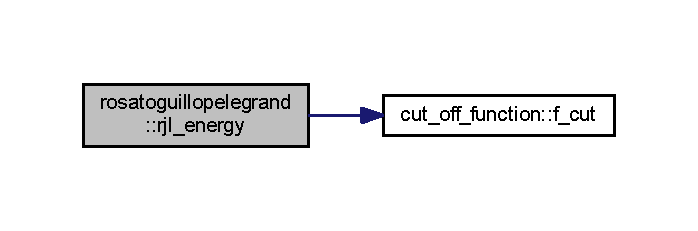
\includegraphics[width=335pt]{namespacerosatoguillopelegrand_a06b6c23e50e301e053ed9ccb60e1ca34_cgraph}
\end{center}
\end{figure}
\mbox{\Hypertarget{namespacerosatoguillopelegrand_a3744fc3d1e6df3ca288ddc43df483ca0}\label{namespacerosatoguillopelegrand_a3744fc3d1e6df3ca288ddc43df483ca0}} 
\index{rosatoguillopelegrand@{rosatoguillopelegrand}!rjl\+\_\+forces@{rjl\+\_\+forces}}
\index{rjl\+\_\+forces@{rjl\+\_\+forces}!rosatoguillopelegrand@{rosatoguillopelegrand}}
\subsubsection{\texorpdfstring{rjl\+\_\+forces()}{rjl\_forces()}}
{\footnotesize\ttfamily subroutine rosatoguillopelegrand\+::rjl\+\_\+forces (\begin{DoxyParamCaption}\item[{type(\mbox{\hyperlink{structmd__general_1_1particles}{particles}})}]{atoms,  }\item[{type(\mbox{\hyperlink{structmd__general_1_1neighbour__list}{neighbour\+\_\+list}})}]{nl,  }\item[{type(\mbox{\hyperlink{structrosatoguillopelegrand_1_1rosatoguillopelegrand__parameters}{rosatoguillopelegrand\+\_\+parameters}})}]{R\+J\+Lp }\end{DoxyParamCaption})}



См. определение в файле Rosato\+Guillope\+Legrand.\+f90 строка 52


\begin{DoxyCode}
52     \textcolor{keywordtype}{type}(RosatoGuillopeLegrand\_parameters):: RJLp
53     \textcolor{keywordtype}{type}(particles)::   atoms
54     \textcolor{keywordtype}{type}(neighbour\_list):: nl
55     \textcolor{keywordtype}{integer}:: i,p
56     \textcolor{keywordtype}{real}:: fc,dfc,Eb(nl%N),expp(nl%neighb\_num\_max,nl%N),expq(nl%neighb\_num\_max,nl%N)
57     
58     \textcolor{comment}{!$OMP PARALLEL firstprivate(i,p,fc,dfc)}
59     \textcolor{comment}{!$OMP DO}
60     \textcolor{keywordflow}{do} i=1,nl%N
61         \textcolor{keywordflow}{do} p=1,nl%nnum(i)
62             \textcolor{keywordflow}{if}( nl%moddr(p,i)<=rjlp%R2 ) \textcolor{keywordflow}{then}
63                 expq(p,i) = exp(-2.*rjlp%q*(nl%moddr(p,i)/rjlp%r0-1.))
64                 expp(p,i) = exp(-rjlp%p*(nl%moddr(p,i)/rjlp%r0-1.))
65 \textcolor{keywordflow}{            endif}
66 \textcolor{keywordflow}{        enddo}
67 \textcolor{keywordflow}{    enddo}
68     \textcolor{comment}{!$OMP END DO}
69     \textcolor{comment}{!$OMP DO    }
70     \textcolor{keywordflow}{do} i=1,nl%N
71         eb(i) = 0.
72         \textcolor{keywordflow}{do} p=1,nl%nnum(i)
73             \textcolor{keywordflow}{if}( nl%moddr(p,i)<=rjlp%R2 ) \textcolor{keywordflow}{then}
74                 eb(i) = eb(i)+expq(p,i)*f\_cut(nl%moddr(p,i),rjlp%R1,rjlp%R2)
75 \textcolor{keywordflow}{            endif}
76 \textcolor{keywordflow}{        enddo}
77         eb(i) = sqrt(eb(i))
78 \textcolor{keywordflow}{    enddo}
79     \textcolor{comment}{!$OMP END DO}
80     \textcolor{comment}{!$OMP DO    }
81     \textcolor{keywordflow}{do} i=1,nl%N
82         \textcolor{keywordflow}{do} p=1,nl%nnum(i)
83             \textcolor{keywordflow}{if}( nl%moddr(p,i)<=rjlp%R2 ) \textcolor{keywordflow}{then}
84                 fc = f\_cut(nl%moddr(p,i),rjlp%R1,rjlp%R2)
85                 dfc = df\_cut(nl%moddr(p,i),rjlp%R1,rjlp%R2)
86                 atoms%forces(:,nl%particle\_index(i)) = atoms%forces(:,nl%particle\_index(i))&
87                 -(2.*rjlp%A0*(rjlp%p/rjlp%r0*fc-dfc*nl%moddr(p,i))*expp(p,i)&
88                 -rjlp%xi*(rjlp%q/rjlp%r0*fc-dfc/2.*nl%moddr(p,i))*(1./eb(i)+1./eb(nl%nlist(p,i)))*expq(p,i)
      )/nl%moddr(p,i)*nl%dr(:,p,i)
89 \textcolor{keywordflow}{            endif}
90 \textcolor{keywordflow}{        enddo}
91 \textcolor{keywordflow}{    enddo}
92     \textcolor{comment}{!$OMP END DO}
93     \textcolor{comment}{!$OMP END PARALLEL}
\end{DoxyCode}
Граф вызовов\+:\nopagebreak
\begin{figure}[H]
\begin{center}
\leavevmode
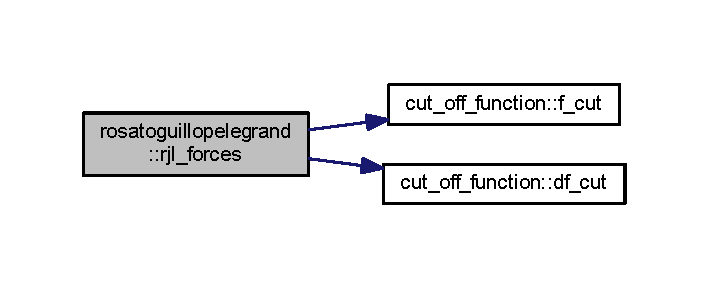
\includegraphics[width=340pt]{namespacerosatoguillopelegrand_a3744fc3d1e6df3ca288ddc43df483ca0_cgraph}
\end{center}
\end{figure}

\hypertarget{namespacetersoffbrenner}{}\section{Модуль tersoffbrenner}
\label{namespacetersoffbrenner}\index{tersoffbrenner@{tersoffbrenner}}
\subsection*{Типы данных}
\begin{DoxyCompactItemize}
\item 
type \mbox{\hyperlink{structtersoffbrenner_1_1tersoffbrenner__parameters}{tersoffbrenner\+\_\+parameters}}
\end{DoxyCompactItemize}
\subsection*{Функции/подпрограммы}
\begin{DoxyCompactItemize}
\item 
subroutine \mbox{\hyperlink{namespacetersoffbrenner_a04beb5c27e136d95b3502f15d39d8ef9}{read\+\_\+tb\+\_\+parameters}} (T\+Bp, filename)
\item 
subroutine \mbox{\hyperlink{namespacetersoffbrenner_a273a6849892363697886b1f1d0f8df93}{tb\+\_\+energy}} (energy, nl, T\+Bp)
\item 
subroutine \mbox{\hyperlink{namespacetersoffbrenner_a1edc8ac251b3fa58026839db4d23f12a}{tb\+\_\+forces}} (atoms, nl, T\+Bp)
\end{DoxyCompactItemize}


\subsection{Функции/подпрограммы}
\mbox{\Hypertarget{namespacetersoffbrenner_a04beb5c27e136d95b3502f15d39d8ef9}\label{namespacetersoffbrenner_a04beb5c27e136d95b3502f15d39d8ef9}} 
\index{tersoffbrenner@{tersoffbrenner}!read\+\_\+tb\+\_\+parameters@{read\+\_\+tb\+\_\+parameters}}
\index{read\+\_\+tb\+\_\+parameters@{read\+\_\+tb\+\_\+parameters}!tersoffbrenner@{tersoffbrenner}}
\subsubsection{\texorpdfstring{read\+\_\+tb\+\_\+parameters()}{read\_tb\_parameters()}}
{\footnotesize\ttfamily subroutine tersoffbrenner\+::read\+\_\+tb\+\_\+parameters (\begin{DoxyParamCaption}\item[{type(\mbox{\hyperlink{structtersoffbrenner_1_1tersoffbrenner__parameters}{tersoffbrenner\+\_\+parameters}})}]{T\+Bp,  }\item[{character($\ast$)}]{filename }\end{DoxyParamCaption})}



См. определение в файле Tersoff\+Brenner.\+f90 строка 14


\begin{DoxyCode}
14     \textcolor{keywordtype}{type}(TersoffBrenner\_parameters):: TBp
15     \textcolor{keywordtype}{character(*)}::  filename
16     
17     \textcolor{keyword}{open}(1,file=filename)
18     \textcolor{keyword}{read}(1,*) tbp%d,tbp%s,tbp%b,tbp%r0,tbp%delt,tbp%a0,tbp%c0,tbp%d0
19     \textcolor{keyword}{read}(1,*) tbp%R1,tbp%R2
20     \textcolor{keyword}{close}(1)
21     tbp%c02 = tbp%c0**2
22     tbp%d02 = tbp%d0**2
23     
\end{DoxyCode}
\mbox{\Hypertarget{namespacetersoffbrenner_a273a6849892363697886b1f1d0f8df93}\label{namespacetersoffbrenner_a273a6849892363697886b1f1d0f8df93}} 
\index{tersoffbrenner@{tersoffbrenner}!tb\+\_\+energy@{tb\+\_\+energy}}
\index{tb\+\_\+energy@{tb\+\_\+energy}!tersoffbrenner@{tersoffbrenner}}
\subsubsection{\texorpdfstring{tb\+\_\+energy()}{tb\_energy()}}
{\footnotesize\ttfamily subroutine tersoffbrenner\+::tb\+\_\+energy (\begin{DoxyParamCaption}\item[{real}]{energy,  }\item[{type(\mbox{\hyperlink{structmd__general_1_1neighbour__list}{neighbour\+\_\+list}})}]{nl,  }\item[{type(\mbox{\hyperlink{structtersoffbrenner_1_1tersoffbrenner__parameters}{tersoffbrenner\+\_\+parameters}})}]{T\+Bp }\end{DoxyParamCaption})}



См. определение в файле Tersoff\+Brenner.\+f90 строка 27


\begin{DoxyCode}
27     \textcolor{keywordtype}{type}(neighbour\_list):: nl
28     \textcolor{keywordtype}{type}(TersoffBrenner\_parameters):: TBp
29     \textcolor{keywordtype}{integer}:: i,p,j,q
30     \textcolor{keywordtype}{real}:: energy,energy\_priv,B(nl%neighb\_num\_max,nl%N),a
31 
32     energy = 0.
33     energy\_priv = 0.
34     \textcolor{comment}{!$OMP PARALLEL firstprivate(energy\_priv,i,p,j,q,a)}
35     \textcolor{comment}{!$OMP DO}
36     \textcolor{keywordflow}{do} i=1,nl%N
37         b(:,i) = 0. \textcolor{comment}{!look rebosc }
38         \textcolor{keywordflow}{do} p=1,nl%nnum(i)
39             \textcolor{comment}{!B(p,i) = 0.}
40             \textcolor{keywordflow}{if} (nl%moddr(p,i)<tbp%R2) \textcolor{keywordflow}{then}
41                 \textcolor{keywordflow}{do} q=1,nl%nnum(i)
42                     \textcolor{keywordflow}{if}(p/=q .AND. nl%moddr(q,i)<tbp%R2) \textcolor{keywordflow}{then}
43                         b(p,i) = b(p,i)+f\_cut(nl%moddr(q,i),tbp%R1,tbp%R2)*&
44                         (1.+tbp%c02/tbp%d02-tbp%c02/(tbp%d02+(1.+sum(nl%dr(:,p,i)*nl%dr(:,q,i))/(nl%moddr(p
      ,i)*nl%moddr(q,i)))**2)) 
45 \textcolor{keywordflow}{                    endif}
46 \textcolor{keywordflow}{                enddo}
47                 b(p,i) = (1.+tbp%a0*b(p,i))**(-tbp%delt)
48 \textcolor{keywordflow}{            endif}
49 \textcolor{keywordflow}{        enddo}
50 \textcolor{keywordflow}{    enddo}
51     \textcolor{comment}{!$OMP END DO    }
52     \textcolor{comment}{!$OMP DO}
53     \textcolor{keywordflow}{do} i=1,nl%N
54         \textcolor{keywordflow}{do} p=1,nl%nnum(i)
55             \textcolor{keywordflow}{if} (nl%moddr(p,i)<tbp%R2) \textcolor{keywordflow}{then}
56                 j = nl%nlist(p,i)
57                 \textcolor{keywordflow}{if} (j>i) \textcolor{keywordflow}{then}
58                     \textcolor{keywordflow}{do} q=1,nl%nnum(j)
59                         \textcolor{keywordflow}{if}(nl%nlist(q,j)==i) \textcolor{keywordflow}{exit}
60 \textcolor{keywordflow}{                    enddo}
61                     a = -sqrt(2.*tbp%s)*tbp%b*(nl%moddr(p,i)-tbp%r0)
62                     energy\_priv = energy\_priv+f\_cut(nl%moddr(p,i),tbp%R1,tbp%R2)*tbp%d/(tbp%s-1.)*(exp(a)-(
      b(p,i)+b(q,j))/2*tbp%s*exp(a/tbp%s))
63 \textcolor{keywordflow}{                endif}
64 \textcolor{keywordflow}{            endif}
65 \textcolor{keywordflow}{        enddo}
66 \textcolor{keywordflow}{    enddo}
67     \textcolor{comment}{!$OMP END DO}
68     \textcolor{comment}{!$OMP ATOMIC}
69         energy = energy+energy\_priv
70     \textcolor{comment}{!$OMP END PARALLEL}
71     
\end{DoxyCode}
Граф вызовов\+:\nopagebreak
\begin{figure}[H]
\begin{center}
\leavevmode
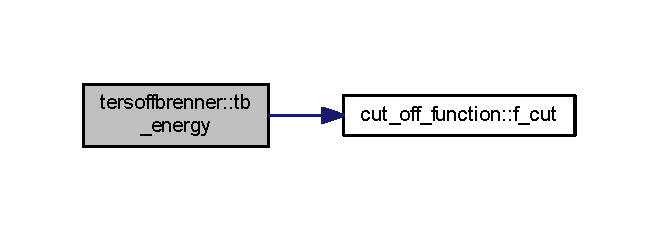
\includegraphics[width=316pt]{namespacetersoffbrenner_a273a6849892363697886b1f1d0f8df93_cgraph}
\end{center}
\end{figure}
\mbox{\Hypertarget{namespacetersoffbrenner_a1edc8ac251b3fa58026839db4d23f12a}\label{namespacetersoffbrenner_a1edc8ac251b3fa58026839db4d23f12a}} 
\index{tersoffbrenner@{tersoffbrenner}!tb\+\_\+forces@{tb\+\_\+forces}}
\index{tb\+\_\+forces@{tb\+\_\+forces}!tersoffbrenner@{tersoffbrenner}}
\subsubsection{\texorpdfstring{tb\+\_\+forces()}{tb\_forces()}}
{\footnotesize\ttfamily subroutine tersoffbrenner\+::tb\+\_\+forces (\begin{DoxyParamCaption}\item[{type(\mbox{\hyperlink{structmd__general_1_1particles}{particles}})}]{atoms,  }\item[{type(\mbox{\hyperlink{structmd__general_1_1neighbour__list}{neighbour\+\_\+list}})}]{nl,  }\item[{type(\mbox{\hyperlink{structtersoffbrenner_1_1tersoffbrenner__parameters}{tersoffbrenner\+\_\+parameters}})}]{T\+Bp }\end{DoxyParamCaption})}



См. определение в файле Tersoff\+Brenner.\+f90 строка 75


\begin{DoxyCode}
75     \textcolor{keywordtype}{type}(particles)::   atoms
76     \textcolor{keywordtype}{type}(neighbour\_list):: nl
77     \textcolor{keywordtype}{type}(TersoffBrenner\_parameters):: TBp
78     \textcolor{keywordtype}{integer}:: i,p,j,q,l
79     \textcolor{keywordtype}{real}:: B(nl%neighb\_num\_max,nl%N),dB(3),a,dff,rr,cosi,f\_c,df\_c
80     
81     \textcolor{comment}{!$OMP PARALLEL firstprivate(i,p,j,q,l,a,dff,rr,cosi,f\_c,df\_c,dB)}
82     \textcolor{comment}{!$OMP DO}
83     \textcolor{keywordflow}{do} i=1,nl%N
84         \textcolor{keywordflow}{do} p=1,nl%nnum(i)
85             b(p,i) = 0.
86             \textcolor{keywordflow}{if} (nl%moddr(p,i)<tbp%R2) \textcolor{keywordflow}{then}
87                 \textcolor{keywordflow}{do} q=1,nl%nnum(i)
88                     \textcolor{keywordflow}{if}(p/=q .AND. nl%moddr(q,i)<tbp%R2) \textcolor{keywordflow}{then}
89                         b(p,i) = b(p,i)+f\_cut(nl%moddr(q,i),tbp%R1,tbp%R2)*&
90                         (1.+tbp%c02/tbp%d02-tbp%c02/(tbp%d02+(1.+sum(nl%dr(:,p,i)*nl%dr(:,q,i))/(nl%moddr(p
      ,i)*nl%moddr(q,i)))**2)) 
91 \textcolor{keywordflow}{                    endif}
92 \textcolor{keywordflow}{                enddo}
93                 b(p,i) = (1.+tbp%a0*b(p,i))**(-tbp%delt)
94 \textcolor{keywordflow}{            endif}
95 \textcolor{keywordflow}{        enddo}
96 \textcolor{keywordflow}{    enddo}
97     \textcolor{comment}{!$OMP END DO    }
98     \textcolor{comment}{!$OMP DO}
99     \textcolor{keywordflow}{do} i=1,nl%N 
100         \textcolor{keywordflow}{do} p=1,nl%nnum(i)
101             db=0.d0
102             \textcolor{keywordflow}{do} q=1,nl%nnum(i)
103                 \textcolor{keywordflow}{if} (p/=q) \textcolor{keywordflow}{then}
104                     rr = 1./nl%moddr(p,i)/nl%moddr(q,i)
105                     cosi = sum(nl%dr(:,p,i)*nl%dr(:,q,i))*rr
106                     db = db+ f\_cut(nl%moddr(q,i),tbp%R1,tbp%R2)*2.d0*tbp%a0*tbp%c02*(1.+cosi)/(tbp%d02+(1.+
      cosi)**2)**2*&
107                         ( (nl%dr(:,p,i)+nl%dr(:,q,i))*rr-cosi*(nl%dr(:,p,i)/nl%moddr(p,i)**2+nl%dr(:,q,i)/
      nl%moddr(q,i)**2) )&
108                         + df\_cut(nl%moddr(q,i),tbp%R1,tbp%R2)*tbp%a0*(1.+tbp%c02/tbp%d02-tbp%c02/(tbp%d02+(
      1.+cosi)**2))*nl%dr(:,q,i)
109 \textcolor{keywordflow}{                endif}
110 \textcolor{keywordflow}{            enddo}
111             db=db*b(p,i)**(1./tbp%delt+1.)
112             j=nl%nlist(p,i)
113             \textcolor{keywordflow}{do} l=1,nl%nnum(j)
114                 \textcolor{keywordflow}{if}(nl%nlist(l,j)==i) \textcolor{keywordflow}{exit}
115 \textcolor{keywordflow}{            enddo}
116             \textcolor{keywordflow}{do} q=1,nl%nnum(j)
117                 \textcolor{keywordflow}{if} (q/=l) \textcolor{keywordflow}{then}
118                     rr = 1./nl%moddr(l,j)/nl%moddr(q,j)
119                     cosi = sum(nl%dr(:,l,j)*nl%dr(:,q,j))*rr 
120                     db = db+(b(l,j)**(1./tbp%delt+1.)*f\_cut(nl%moddr(q,j),tbp%R1,tbp%R2)*&
121                         2.*tbp%a0*tbp%c02*(1.+cosi)/(tbp%d02+(1.+cosi)**2)**2)*(-nl%dr(:,q,j)*rr + cosi*nl
      %dr(:,l,j)/nl%moddr(l,j)**2)
122 \textcolor{keywordflow}{                endif}
123 \textcolor{keywordflow}{            enddo}
124             db = db*(-tbp%delt)/2.
125             \textcolor{keywordflow}{if} (nl%moddr(p,i)<tbp%R2) \textcolor{keywordflow}{then}
126                 f\_c = f\_cut(nl%moddr(p,i),tbp%R1,tbp%R2)
127                 dff = df\_cut(nl%moddr(p,i),tbp%R1,tbp%R2)/f\_c
128                 a = -sqrt(2.*tbp%s)*tbp%b*(nl%moddr(p,i)-tbp%r0)
129                 atoms%forces(:,nl%particle\_index(i)) = atoms%forces(:,nl%particle\_index(i))+&
130                 f\_c*tbp%d/(tbp%s-1.)*((nl%dr(:,p,i)*dff-sqrt(2.*tbp%s)*tbp%b/nl%moddr(p,i)*nl%dr(:,p,i))*
      exp(a)&
131                 -( db+(b(p,i)+b(l,j))/2*(nl%dr(:,p,i)*dff-sqrt(2./tbp%s)*tbp%b/nl%moddr(p,i)*nl%dr(:,p,i)) 
      )*tbp%s*exp(a/tbp%s))
132 \textcolor{keywordflow}{            endif}
133             \textcolor{keywordflow}{do} q=1,nl%nnum(j)
134                 \textcolor{keywordflow}{if} (q/=l) \textcolor{keywordflow}{then}  
135                     f\_c = f\_cut(nl%moddr(l,j),tbp%R1,tbp%R2)
136                     df\_c = df\_cut(nl%moddr(l,j),tbp%R1,tbp%R2)
137                     rr = 1./nl%moddr(l,j)/nl%moddr(q,j)
138                     cosi = sum(nl%dr(:,l,j)*nl%dr(:,q,j))*rr                
139                     atoms%forces(:,nl%particle\_index(i)) = atoms%forces(:,nl%particle\_index(i))+tbp%delt/2*
      b(q,j)**(1./tbp%delt+1.)*&
140                     ( f\_c*2.*tbp%a0*tbp%c02*(1.+cosi)/(tbp%d02+(1.+cosi)**2)**2 *( -nl%dr(:,q,j)*rr + cosi*
      nl%dr(:,l,j)/nl%moddr(l,j)**2 )+&
141                     nl%dr(:,p,i)*df\_c*tbp%a0*(1.+tbp%c02/tbp%d02-tbp%c02/(tbp%d02+(1.+cosi)**2)) )*&
142                     f\_cut(nl%moddr(q,j),tbp%R1,tbp%R2)*tbp%d/(tbp%s-1.)*tbp%s*exp(-sqrt(2.*tbp%s)*tbp%b*(nl
      %moddr(q,j)-tbp%r0)/tbp%s)
143 \textcolor{keywordflow}{                endif}
144 \textcolor{keywordflow}{            enddo}       
145 \textcolor{keywordflow}{        enddo}
146 \textcolor{keywordflow}{    enddo}
147     \textcolor{comment}{!$OMP END DO}
148     \textcolor{comment}{!$OMP END PARALLEL}
149     
\end{DoxyCode}
Граф вызовов\+:\nopagebreak
\begin{figure}[H]
\begin{center}
\leavevmode
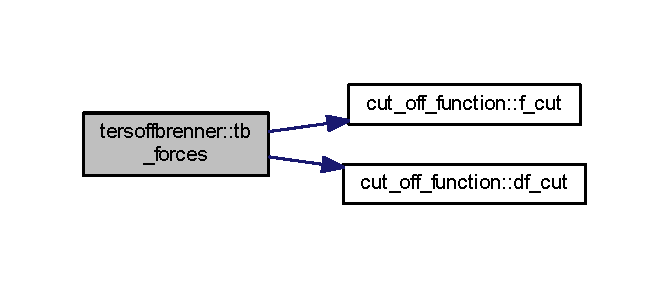
\includegraphics[width=321pt]{namespacetersoffbrenner_a1edc8ac251b3fa58026839db4d23f12a_cgraph}
\end{center}
\end{figure}

\chapter{Оглавление типов данных}
\hypertarget{structmd__general_1_1integrator__params}{}\section{md\+\_\+general\+:\+:integrator\+\_\+params Шаблон типа}
\label{structmd__general_1_1integrator__params}\index{md\+\_\+general\+::integrator\+\_\+params@{md\+\_\+general\+::integrator\+\_\+params}}
\subsection*{Открытые атрибуты}
\begin{DoxyCompactItemize}
\item 
integer \mbox{\hyperlink{structmd__general_1_1integrator__params_a429731dee807f3669a8cd4f8d1c03669}{l}}
\item 
integer \mbox{\hyperlink{structmd__general_1_1integrator__params_a9ccbea50d63a4ed071c21f441e12ebbf}{period\+\_\+snapshot}}
\item 
integer \mbox{\hyperlink{structmd__general_1_1integrator__params_a80455167f3d94737a72d349c78516dcb}{period\+\_\+log}}
\item 
real \mbox{\hyperlink{structmd__general_1_1integrator__params_a421afffa09e4c728d4a2954d9fe59a49}{dt}}
\item 
character(len=32) \mbox{\hyperlink{structmd__general_1_1integrator__params_a39acd9f053ea08a505f545789367a90c}{int\+\_\+name}}
\end{DoxyCompactItemize}


\subsection{Подробное описание}


См. определение в файле md\+\_\+general.\+f90 строка 37



\subsection{Данные класса}
\mbox{\Hypertarget{structmd__general_1_1integrator__params_a421afffa09e4c728d4a2954d9fe59a49}\label{structmd__general_1_1integrator__params_a421afffa09e4c728d4a2954d9fe59a49}} 
\index{md\+\_\+general\+::integrator\+\_\+params@{md\+\_\+general\+::integrator\+\_\+params}!dt@{dt}}
\index{dt@{dt}!md\+\_\+general\+::integrator\+\_\+params@{md\+\_\+general\+::integrator\+\_\+params}}
\subsubsection{\texorpdfstring{dt}{dt}}
{\footnotesize\ttfamily real md\+\_\+general\+::integrator\+\_\+params\+::dt}



См. определение в файле md\+\_\+general.\+f90 строка 39


\begin{DoxyCode}
39     \textcolor{keywordtype}{real}:: dt
\end{DoxyCode}
\mbox{\Hypertarget{structmd__general_1_1integrator__params_a39acd9f053ea08a505f545789367a90c}\label{structmd__general_1_1integrator__params_a39acd9f053ea08a505f545789367a90c}} 
\index{md\+\_\+general\+::integrator\+\_\+params@{md\+\_\+general\+::integrator\+\_\+params}!int\+\_\+name@{int\+\_\+name}}
\index{int\+\_\+name@{int\+\_\+name}!md\+\_\+general\+::integrator\+\_\+params@{md\+\_\+general\+::integrator\+\_\+params}}
\subsubsection{\texorpdfstring{int\+\_\+name}{int\_name}}
{\footnotesize\ttfamily character(len=32) md\+\_\+general\+::integrator\+\_\+params\+::int\+\_\+name}



См. определение в файле md\+\_\+general.\+f90 строка 40


\begin{DoxyCode}
40     \textcolor{keywordtype}{character(len=32)}:: int\_name
\end{DoxyCode}
\mbox{\Hypertarget{structmd__general_1_1integrator__params_a429731dee807f3669a8cd4f8d1c03669}\label{structmd__general_1_1integrator__params_a429731dee807f3669a8cd4f8d1c03669}} 
\index{md\+\_\+general\+::integrator\+\_\+params@{md\+\_\+general\+::integrator\+\_\+params}!l@{l}}
\index{l@{l}!md\+\_\+general\+::integrator\+\_\+params@{md\+\_\+general\+::integrator\+\_\+params}}
\subsubsection{\texorpdfstring{l}{l}}
{\footnotesize\ttfamily integer md\+\_\+general\+::integrator\+\_\+params\+::l}



См. определение в файле md\+\_\+general.\+f90 строка 38


\begin{DoxyCode}
38     \textcolor{keywordtype}{integer}:: l,period\_snapshot,period\_log
\end{DoxyCode}
\mbox{\Hypertarget{structmd__general_1_1integrator__params_a80455167f3d94737a72d349c78516dcb}\label{structmd__general_1_1integrator__params_a80455167f3d94737a72d349c78516dcb}} 
\index{md\+\_\+general\+::integrator\+\_\+params@{md\+\_\+general\+::integrator\+\_\+params}!period\+\_\+log@{period\+\_\+log}}
\index{period\+\_\+log@{period\+\_\+log}!md\+\_\+general\+::integrator\+\_\+params@{md\+\_\+general\+::integrator\+\_\+params}}
\subsubsection{\texorpdfstring{period\+\_\+log}{period\_log}}
{\footnotesize\ttfamily integer md\+\_\+general\+::integrator\+\_\+params\+::period\+\_\+log}



См. определение в файле md\+\_\+general.\+f90 строка 38

\mbox{\Hypertarget{structmd__general_1_1integrator__params_a9ccbea50d63a4ed071c21f441e12ebbf}\label{structmd__general_1_1integrator__params_a9ccbea50d63a4ed071c21f441e12ebbf}} 
\index{md\+\_\+general\+::integrator\+\_\+params@{md\+\_\+general\+::integrator\+\_\+params}!period\+\_\+snapshot@{period\+\_\+snapshot}}
\index{period\+\_\+snapshot@{period\+\_\+snapshot}!md\+\_\+general\+::integrator\+\_\+params@{md\+\_\+general\+::integrator\+\_\+params}}
\subsubsection{\texorpdfstring{period\+\_\+snapshot}{period\_snapshot}}
{\footnotesize\ttfamily integer md\+\_\+general\+::integrator\+\_\+params\+::period\+\_\+snapshot}



См. определение в файле md\+\_\+general.\+f90 строка 38



Документация по типу сгенерирована на основе следующего файла\+:\begin{DoxyCompactItemize}
\item 
M\+O\+L\+E\+C\+U\+L\+A\+R\+\_\+\+D\+Y\+N\+A\+M\+I\+C\+S/\mbox{\hyperlink{md__general_8f90}{md\+\_\+general.\+f90}}\end{DoxyCompactItemize}

\hypertarget{structmd__interactions_1_1interaction}{}\section{md\+\_\+interactions\+:\+:interaction Шаблон типа}
\label{structmd__interactions_1_1interaction}\index{md\+\_\+interactions\+::interaction@{md\+\_\+interactions\+::interaction}}


Граф связей класса md\+\_\+interactions\+:\+:interaction\+:\nopagebreak
\begin{figure}[H]
\begin{center}
\leavevmode
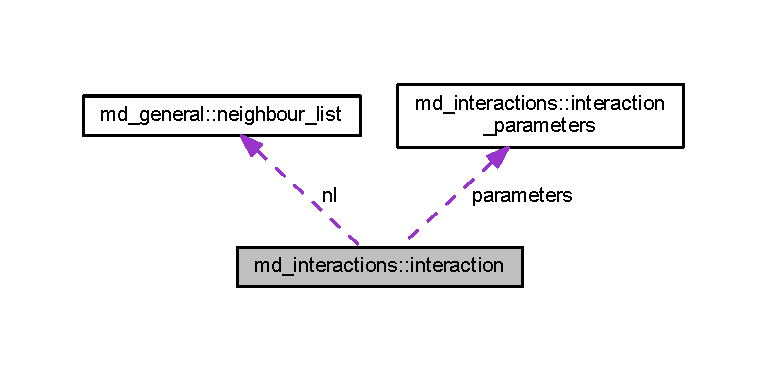
\includegraphics[width=350pt]{structmd__interactions_1_1interaction__coll__graph}
\end{center}
\end{figure}
\subsection*{Открытые атрибуты}
\begin{DoxyCompactItemize}
\item 
integer \mbox{\hyperlink{structmd__interactions_1_1interaction_a45da5fb326e67bc08da38f1cc7b5ff2e}{nl\+\_\+n}}
\item 
integer \mbox{\hyperlink{structmd__interactions_1_1interaction_a1650598e16e38fec2ea5bd093b7cc634}{neib\+\_\+order}}
\item 
integer, dimension(\+:), allocatable \mbox{\hyperlink{structmd__interactions_1_1interaction_a7780370c71abfd1418aba1cc0037f2d1}{group\+\_\+nums}}
\item 
type(\mbox{\hyperlink{structmd__general_1_1neighbour__list}{neighbour\+\_\+list}}), dimension(\+:), allocatable \mbox{\hyperlink{structmd__interactions_1_1interaction_a43d6b246e83e0f832461d029fc922de6}{nl}}
\item 
real \mbox{\hyperlink{structmd__interactions_1_1interaction_a3a150970039b7be4b08b249e30d695e9}{energy}}
\item 
character(len=32) \mbox{\hyperlink{structmd__interactions_1_1interaction_a098dcff72c607d6b5e6a4f0f522b56ed}{interaction\+\_\+name}}
\item 
character(len=32) \mbox{\hyperlink{structmd__interactions_1_1interaction_a1ed21689035f3b5b3bae8aec62a081df}{parameters\+\_\+file}}
\item 
type(\mbox{\hyperlink{structmd__interactions_1_1interaction__parameters}{interaction\+\_\+parameters}}) \mbox{\hyperlink{structmd__interactions_1_1interaction_ab2041dbe838781954511d4738535fa98}{parameters}}
\item 
logical \mbox{\hyperlink{structmd__interactions_1_1interaction_a54ce703312ec9215da8f704c0134814b}{numerical\+\_\+force}}
\end{DoxyCompactItemize}


\subsection{Подробное описание}


См. определение в файле md\+\_\+interactions.\+f90 строка 26



\subsection{Данные класса}
\mbox{\Hypertarget{structmd__interactions_1_1interaction_a3a150970039b7be4b08b249e30d695e9}\label{structmd__interactions_1_1interaction_a3a150970039b7be4b08b249e30d695e9}} 
\index{md\+\_\+interactions\+::interaction@{md\+\_\+interactions\+::interaction}!energy@{energy}}
\index{energy@{energy}!md\+\_\+interactions\+::interaction@{md\+\_\+interactions\+::interaction}}
\subsubsection{\texorpdfstring{energy}{energy}}
{\footnotesize\ttfamily real md\+\_\+interactions\+::interaction\+::energy}



См. определение в файле md\+\_\+interactions.\+f90 строка 30


\begin{DoxyCode}
30     \textcolor{keywordtype}{real}:: energy
\end{DoxyCode}
\mbox{\Hypertarget{structmd__interactions_1_1interaction_a7780370c71abfd1418aba1cc0037f2d1}\label{structmd__interactions_1_1interaction_a7780370c71abfd1418aba1cc0037f2d1}} 
\index{md\+\_\+interactions\+::interaction@{md\+\_\+interactions\+::interaction}!group\+\_\+nums@{group\+\_\+nums}}
\index{group\+\_\+nums@{group\+\_\+nums}!md\+\_\+interactions\+::interaction@{md\+\_\+interactions\+::interaction}}
\subsubsection{\texorpdfstring{group\+\_\+nums}{group\_nums}}
{\footnotesize\ttfamily integer, dimension(\+:), allocatable md\+\_\+interactions\+::interaction\+::group\+\_\+nums}



См. определение в файле md\+\_\+interactions.\+f90 строка 28


\begin{DoxyCode}
28     \textcolor{keywordtype}{integer},\textcolor{keywordtype}{allocatable}:: group\_nums(:)
\end{DoxyCode}
\mbox{\Hypertarget{structmd__interactions_1_1interaction_a098dcff72c607d6b5e6a4f0f522b56ed}\label{structmd__interactions_1_1interaction_a098dcff72c607d6b5e6a4f0f522b56ed}} 
\index{md\+\_\+interactions\+::interaction@{md\+\_\+interactions\+::interaction}!interaction\+\_\+name@{interaction\+\_\+name}}
\index{interaction\+\_\+name@{interaction\+\_\+name}!md\+\_\+interactions\+::interaction@{md\+\_\+interactions\+::interaction}}
\subsubsection{\texorpdfstring{interaction\+\_\+name}{interaction\_name}}
{\footnotesize\ttfamily character(len=32) md\+\_\+interactions\+::interaction\+::interaction\+\_\+name}



См. определение в файле md\+\_\+interactions.\+f90 строка 31


\begin{DoxyCode}
31     \textcolor{keywordtype}{character(len=32)}:: interaction\_name,parameters\_file
\end{DoxyCode}
\mbox{\Hypertarget{structmd__interactions_1_1interaction_a1650598e16e38fec2ea5bd093b7cc634}\label{structmd__interactions_1_1interaction_a1650598e16e38fec2ea5bd093b7cc634}} 
\index{md\+\_\+interactions\+::interaction@{md\+\_\+interactions\+::interaction}!neib\+\_\+order@{neib\+\_\+order}}
\index{neib\+\_\+order@{neib\+\_\+order}!md\+\_\+interactions\+::interaction@{md\+\_\+interactions\+::interaction}}
\subsubsection{\texorpdfstring{neib\+\_\+order}{neib\_order}}
{\footnotesize\ttfamily integer md\+\_\+interactions\+::interaction\+::neib\+\_\+order}



См. определение в файле md\+\_\+interactions.\+f90 строка 27

\mbox{\Hypertarget{structmd__interactions_1_1interaction_a43d6b246e83e0f832461d029fc922de6}\label{structmd__interactions_1_1interaction_a43d6b246e83e0f832461d029fc922de6}} 
\index{md\+\_\+interactions\+::interaction@{md\+\_\+interactions\+::interaction}!nl@{nl}}
\index{nl@{nl}!md\+\_\+interactions\+::interaction@{md\+\_\+interactions\+::interaction}}
\subsubsection{\texorpdfstring{nl}{nl}}
{\footnotesize\ttfamily type(\mbox{\hyperlink{structmd__general_1_1neighbour__list}{neighbour\+\_\+list}}), dimension(\+:), allocatable md\+\_\+interactions\+::interaction\+::nl}



См. определение в файле md\+\_\+interactions.\+f90 строка 29


\begin{DoxyCode}
29     \textcolor{keywordtype}{type}(neighbour\_list),\textcolor{keywordtype}{allocatable}:: nl(:)
\end{DoxyCode}
\mbox{\Hypertarget{structmd__interactions_1_1interaction_a45da5fb326e67bc08da38f1cc7b5ff2e}\label{structmd__interactions_1_1interaction_a45da5fb326e67bc08da38f1cc7b5ff2e}} 
\index{md\+\_\+interactions\+::interaction@{md\+\_\+interactions\+::interaction}!nl\+\_\+n@{nl\+\_\+n}}
\index{nl\+\_\+n@{nl\+\_\+n}!md\+\_\+interactions\+::interaction@{md\+\_\+interactions\+::interaction}}
\subsubsection{\texorpdfstring{nl\+\_\+n}{nl\_n}}
{\footnotesize\ttfamily integer md\+\_\+interactions\+::interaction\+::nl\+\_\+n}



См. определение в файле md\+\_\+interactions.\+f90 строка 27


\begin{DoxyCode}
27     \textcolor{keywordtype}{integer}:: nl\_n,neib\_order
\end{DoxyCode}
\mbox{\Hypertarget{structmd__interactions_1_1interaction_a54ce703312ec9215da8f704c0134814b}\label{structmd__interactions_1_1interaction_a54ce703312ec9215da8f704c0134814b}} 
\index{md\+\_\+interactions\+::interaction@{md\+\_\+interactions\+::interaction}!numerical\+\_\+force@{numerical\+\_\+force}}
\index{numerical\+\_\+force@{numerical\+\_\+force}!md\+\_\+interactions\+::interaction@{md\+\_\+interactions\+::interaction}}
\subsubsection{\texorpdfstring{numerical\+\_\+force}{numerical\_force}}
{\footnotesize\ttfamily logical md\+\_\+interactions\+::interaction\+::numerical\+\_\+force}



См. определение в файле md\+\_\+interactions.\+f90 строка 33


\begin{DoxyCode}
33     \textcolor{keywordtype}{logical}:: numerical\_force
\end{DoxyCode}
\mbox{\Hypertarget{structmd__interactions_1_1interaction_ab2041dbe838781954511d4738535fa98}\label{structmd__interactions_1_1interaction_ab2041dbe838781954511d4738535fa98}} 
\index{md\+\_\+interactions\+::interaction@{md\+\_\+interactions\+::interaction}!parameters@{parameters}}
\index{parameters@{parameters}!md\+\_\+interactions\+::interaction@{md\+\_\+interactions\+::interaction}}
\subsubsection{\texorpdfstring{parameters}{parameters}}
{\footnotesize\ttfamily type(\mbox{\hyperlink{structmd__interactions_1_1interaction__parameters}{interaction\+\_\+parameters}}) md\+\_\+interactions\+::interaction\+::parameters}



См. определение в файле md\+\_\+interactions.\+f90 строка 32


\begin{DoxyCode}
32     \textcolor{keywordtype}{type}(interaction\_parameters) :: parameters
\end{DoxyCode}
\mbox{\Hypertarget{structmd__interactions_1_1interaction_a1ed21689035f3b5b3bae8aec62a081df}\label{structmd__interactions_1_1interaction_a1ed21689035f3b5b3bae8aec62a081df}} 
\index{md\+\_\+interactions\+::interaction@{md\+\_\+interactions\+::interaction}!parameters\+\_\+file@{parameters\+\_\+file}}
\index{parameters\+\_\+file@{parameters\+\_\+file}!md\+\_\+interactions\+::interaction@{md\+\_\+interactions\+::interaction}}
\subsubsection{\texorpdfstring{parameters\+\_\+file}{parameters\_file}}
{\footnotesize\ttfamily character(len=32) md\+\_\+interactions\+::interaction\+::parameters\+\_\+file}



См. определение в файле md\+\_\+interactions.\+f90 строка 31



Документация по типу сгенерирована на основе следующего файла\+:\begin{DoxyCompactItemize}
\item 
M\+O\+L\+E\+C\+U\+L\+A\+R\+\_\+\+D\+Y\+N\+A\+M\+I\+C\+S/\mbox{\hyperlink{md__interactions_8f90}{md\+\_\+interactions.\+f90}}\end{DoxyCompactItemize}

\hypertarget{structmd__interactions_1_1interaction__parameters}{}\section{md\+\_\+interactions\+:\+:interaction\+\_\+parameters Шаблон типа}
\label{structmd__interactions_1_1interaction__parameters}\index{md\+\_\+interactions\+::interaction\+\_\+parameters@{md\+\_\+interactions\+::interaction\+\_\+parameters}}
\subsection*{Открытые атрибуты}
\begin{DoxyCompactItemize}
\item 
type(lennardjones\+\_\+parameters), dimension(\+:), allocatable \mbox{\hyperlink{structmd__interactions_1_1interaction__parameters_a17105aae3c1c70e8e38f8df76a4d1c57}{lj}}
\item 
type(lennardjones1g\+\_\+parameters), dimension(\+:), allocatable \mbox{\hyperlink{structmd__interactions_1_1interaction__parameters_aa915e6095a7f0f3c11cd2c25cea344c9}{lj1g}}
\item 
type(lennardjonescosine\+\_\+parameters), dimension(\+:), allocatable \mbox{\hyperlink{structmd__interactions_1_1interaction__parameters_aecba06e4ab6722165fa45ccbe7bc5408}{ljc}}
\item 
type(morsecosine\+\_\+parameters), dimension(\+:), allocatable \mbox{\hyperlink{structmd__interactions_1_1interaction__parameters_a38771bf0f6c0cd4ac46151171dd2b824}{morsec}}
\item 
type(rosatoguillopelegrand\+\_\+parameters), dimension(\+:), allocatable \mbox{\hyperlink{structmd__interactions_1_1interaction__parameters_ae23b19b674151370a0cb9b6b24b8ea86}{rjl}}
\item 
type(tersoffbrenner\+\_\+parameters), dimension(\+:), allocatable \mbox{\hyperlink{structmd__interactions_1_1interaction__parameters_acb1a5443eba1a0c63403bc9e8dc73cfd}{tb}}
\item 
type(rebosc\+\_\+parameters), dimension(\+:), allocatable \mbox{\hyperlink{structmd__interactions_1_1interaction__parameters_a165970e0061960e267d6812368a16ca1}{rebosc}}
\end{DoxyCompactItemize}


\subsection{Подробное описание}


См. определение в файле md\+\_\+interactions.\+f90 строка 15



\subsection{Данные класса}
\mbox{\Hypertarget{structmd__interactions_1_1interaction__parameters_a17105aae3c1c70e8e38f8df76a4d1c57}\label{structmd__interactions_1_1interaction__parameters_a17105aae3c1c70e8e38f8df76a4d1c57}} 
\index{md\+\_\+interactions\+::interaction\+\_\+parameters@{md\+\_\+interactions\+::interaction\+\_\+parameters}!lj@{lj}}
\index{lj@{lj}!md\+\_\+interactions\+::interaction\+\_\+parameters@{md\+\_\+interactions\+::interaction\+\_\+parameters}}
\subsubsection{\texorpdfstring{lj}{lj}}
{\footnotesize\ttfamily type(lennardjones\+\_\+parameters), dimension(\+:), allocatable md\+\_\+interactions\+::interaction\+\_\+parameters\+::lj}



См. определение в файле md\+\_\+interactions.\+f90 строка 16


\begin{DoxyCode}
16     \textcolor{keywordtype}{type}(LennardJones\_parameters),allocatable           :: LJ(:)
\end{DoxyCode}
\mbox{\Hypertarget{structmd__interactions_1_1interaction__parameters_aa915e6095a7f0f3c11cd2c25cea344c9}\label{structmd__interactions_1_1interaction__parameters_aa915e6095a7f0f3c11cd2c25cea344c9}} 
\index{md\+\_\+interactions\+::interaction\+\_\+parameters@{md\+\_\+interactions\+::interaction\+\_\+parameters}!lj1g@{lj1g}}
\index{lj1g@{lj1g}!md\+\_\+interactions\+::interaction\+\_\+parameters@{md\+\_\+interactions\+::interaction\+\_\+parameters}}
\subsubsection{\texorpdfstring{lj1g}{lj1g}}
{\footnotesize\ttfamily type(lennardjones1g\+\_\+parameters), dimension(\+:), allocatable md\+\_\+interactions\+::interaction\+\_\+parameters\+::lj1g}



См. определение в файле md\+\_\+interactions.\+f90 строка 17


\begin{DoxyCode}
17     \textcolor{keywordtype}{type}(LennardJones1g\_parameters),allocatable         :: LJ1g(:)
\end{DoxyCode}
\mbox{\Hypertarget{structmd__interactions_1_1interaction__parameters_aecba06e4ab6722165fa45ccbe7bc5408}\label{structmd__interactions_1_1interaction__parameters_aecba06e4ab6722165fa45ccbe7bc5408}} 
\index{md\+\_\+interactions\+::interaction\+\_\+parameters@{md\+\_\+interactions\+::interaction\+\_\+parameters}!ljc@{ljc}}
\index{ljc@{ljc}!md\+\_\+interactions\+::interaction\+\_\+parameters@{md\+\_\+interactions\+::interaction\+\_\+parameters}}
\subsubsection{\texorpdfstring{ljc}{ljc}}
{\footnotesize\ttfamily type(lennardjonescosine\+\_\+parameters), dimension(\+:), allocatable md\+\_\+interactions\+::interaction\+\_\+parameters\+::ljc}



См. определение в файле md\+\_\+interactions.\+f90 строка 19


\begin{DoxyCode}
19     \textcolor{keywordtype}{type}(LennardJonesCosine\_parameters),allocatable     :: LJC(:)
\end{DoxyCode}
\mbox{\Hypertarget{structmd__interactions_1_1interaction__parameters_a38771bf0f6c0cd4ac46151171dd2b824}\label{structmd__interactions_1_1interaction__parameters_a38771bf0f6c0cd4ac46151171dd2b824}} 
\index{md\+\_\+interactions\+::interaction\+\_\+parameters@{md\+\_\+interactions\+::interaction\+\_\+parameters}!morsec@{morsec}}
\index{morsec@{morsec}!md\+\_\+interactions\+::interaction\+\_\+parameters@{md\+\_\+interactions\+::interaction\+\_\+parameters}}
\subsubsection{\texorpdfstring{morsec}{morsec}}
{\footnotesize\ttfamily type(morsecosine\+\_\+parameters), dimension(\+:), allocatable md\+\_\+interactions\+::interaction\+\_\+parameters\+::morsec}



См. определение в файле md\+\_\+interactions.\+f90 строка 20


\begin{DoxyCode}
20     \textcolor{keywordtype}{type}(MorseCosine\_parameters),allocatable            :: MorseC(:)
\end{DoxyCode}
\mbox{\Hypertarget{structmd__interactions_1_1interaction__parameters_a165970e0061960e267d6812368a16ca1}\label{structmd__interactions_1_1interaction__parameters_a165970e0061960e267d6812368a16ca1}} 
\index{md\+\_\+interactions\+::interaction\+\_\+parameters@{md\+\_\+interactions\+::interaction\+\_\+parameters}!rebosc@{rebosc}}
\index{rebosc@{rebosc}!md\+\_\+interactions\+::interaction\+\_\+parameters@{md\+\_\+interactions\+::interaction\+\_\+parameters}}
\subsubsection{\texorpdfstring{rebosc}{rebosc}}
{\footnotesize\ttfamily type(rebosc\+\_\+parameters), dimension(\+:), allocatable md\+\_\+interactions\+::interaction\+\_\+parameters\+::rebosc}



См. определение в файле md\+\_\+interactions.\+f90 строка 23


\begin{DoxyCode}
23     \textcolor{keywordtype}{type}(REBOsc\_parameters),allocatable                 :: REBOsc(:)
\end{DoxyCode}
\mbox{\Hypertarget{structmd__interactions_1_1interaction__parameters_ae23b19b674151370a0cb9b6b24b8ea86}\label{structmd__interactions_1_1interaction__parameters_ae23b19b674151370a0cb9b6b24b8ea86}} 
\index{md\+\_\+interactions\+::interaction\+\_\+parameters@{md\+\_\+interactions\+::interaction\+\_\+parameters}!rjl@{rjl}}
\index{rjl@{rjl}!md\+\_\+interactions\+::interaction\+\_\+parameters@{md\+\_\+interactions\+::interaction\+\_\+parameters}}
\subsubsection{\texorpdfstring{rjl}{rjl}}
{\footnotesize\ttfamily type(rosatoguillopelegrand\+\_\+parameters), dimension(\+:), allocatable md\+\_\+interactions\+::interaction\+\_\+parameters\+::rjl}



См. определение в файле md\+\_\+interactions.\+f90 строка 21


\begin{DoxyCode}
21     \textcolor{keywordtype}{type}(RosatoGuillopeLegrand\_parameters),allocatable  :: RJL(:)
\end{DoxyCode}
\mbox{\Hypertarget{structmd__interactions_1_1interaction__parameters_acb1a5443eba1a0c63403bc9e8dc73cfd}\label{structmd__interactions_1_1interaction__parameters_acb1a5443eba1a0c63403bc9e8dc73cfd}} 
\index{md\+\_\+interactions\+::interaction\+\_\+parameters@{md\+\_\+interactions\+::interaction\+\_\+parameters}!tb@{tb}}
\index{tb@{tb}!md\+\_\+interactions\+::interaction\+\_\+parameters@{md\+\_\+interactions\+::interaction\+\_\+parameters}}
\subsubsection{\texorpdfstring{tb}{tb}}
{\footnotesize\ttfamily type(tersoffbrenner\+\_\+parameters), dimension(\+:), allocatable md\+\_\+interactions\+::interaction\+\_\+parameters\+::tb}



См. определение в файле md\+\_\+interactions.\+f90 строка 22


\begin{DoxyCode}
22     \textcolor{keywordtype}{type}(TersoffBrenner\_parameters),allocatable         :: TB(:)
\end{DoxyCode}


Документация по типу сгенерирована на основе следующего файла\+:\begin{DoxyCompactItemize}
\item 
M\+O\+L\+E\+C\+U\+L\+A\+R\+\_\+\+D\+Y\+N\+A\+M\+I\+C\+S/\mbox{\hyperlink{md__interactions_8f90}{md\+\_\+interactions.\+f90}}\end{DoxyCompactItemize}

\hypertarget{structlennardjones__1g_1_1lennardjones1g__parameters}{}\section{lennardjones\+\_\+1g\+:\+:lennardjones1g\+\_\+parameters Шаблон типа}
\label{structlennardjones__1g_1_1lennardjones1g__parameters}\index{lennardjones\+\_\+1g\+::lennardjones1g\+\_\+parameters@{lennardjones\+\_\+1g\+::lennardjones1g\+\_\+parameters}}
\subsection*{Открытые атрибуты}
\begin{DoxyCompactItemize}
\item 
real \mbox{\hyperlink{structlennardjones__1g_1_1lennardjones1g__parameters_a750108d359052e9d7626761bb6e0dfaa}{eps}}
\item 
real \mbox{\hyperlink{structlennardjones__1g_1_1lennardjones1g__parameters_a88ba8f2d417b65ea5e0aa07171954a15}{sig}}
\item 
real \mbox{\hyperlink{structlennardjones__1g_1_1lennardjones1g__parameters_a7c4b6140f75f4eb0f8c00b15b01728a9}{r1}}
\item 
real \mbox{\hyperlink{structlennardjones__1g_1_1lennardjones1g__parameters_a5f7fe6b683aacc2014ef8573e527508b}{r2}}
\item 
real \mbox{\hyperlink{structlennardjones__1g_1_1lennardjones1g__parameters_a90483776bbf758f100d79cc4902c3ced}{c6}}
\item 
real \mbox{\hyperlink{structlennardjones__1g_1_1lennardjones1g__parameters_a44cabdf352bfd6ae6eda9f03bb956db2}{c12}}
\item 
real \mbox{\hyperlink{structlennardjones__1g_1_1lennardjones1g__parameters_a350fbbd96a4bc274f86ff08921f6b287}{c6t6}}
\item 
real \mbox{\hyperlink{structlennardjones__1g_1_1lennardjones1g__parameters_a8251b4f08d7fd30d611cfa67bb6d0b5e}{c12t12}}
\end{DoxyCompactItemize}


\subsection{Подробное описание}


См. определение в файле Lennard\+Jones\+\_\+1g.\+f90 строка 7



\subsection{Данные класса}
\mbox{\Hypertarget{structlennardjones__1g_1_1lennardjones1g__parameters_a44cabdf352bfd6ae6eda9f03bb956db2}\label{structlennardjones__1g_1_1lennardjones1g__parameters_a44cabdf352bfd6ae6eda9f03bb956db2}} 
\index{lennardjones\+\_\+1g\+::lennardjones1g\+\_\+parameters@{lennardjones\+\_\+1g\+::lennardjones1g\+\_\+parameters}!c12@{c12}}
\index{c12@{c12}!lennardjones\+\_\+1g\+::lennardjones1g\+\_\+parameters@{lennardjones\+\_\+1g\+::lennardjones1g\+\_\+parameters}}
\subsubsection{\texorpdfstring{c12}{c12}}
{\footnotesize\ttfamily real lennardjones\+\_\+1g\+::lennardjones1g\+\_\+parameters\+::c12}



См. определение в файле Lennard\+Jones\+\_\+1g.\+f90 строка 8

\mbox{\Hypertarget{structlennardjones__1g_1_1lennardjones1g__parameters_a8251b4f08d7fd30d611cfa67bb6d0b5e}\label{structlennardjones__1g_1_1lennardjones1g__parameters_a8251b4f08d7fd30d611cfa67bb6d0b5e}} 
\index{lennardjones\+\_\+1g\+::lennardjones1g\+\_\+parameters@{lennardjones\+\_\+1g\+::lennardjones1g\+\_\+parameters}!c12t12@{c12t12}}
\index{c12t12@{c12t12}!lennardjones\+\_\+1g\+::lennardjones1g\+\_\+parameters@{lennardjones\+\_\+1g\+::lennardjones1g\+\_\+parameters}}
\subsubsection{\texorpdfstring{c12t12}{c12t12}}
{\footnotesize\ttfamily real lennardjones\+\_\+1g\+::lennardjones1g\+\_\+parameters\+::c12t12}



См. определение в файле Lennard\+Jones\+\_\+1g.\+f90 строка 8

\mbox{\Hypertarget{structlennardjones__1g_1_1lennardjones1g__parameters_a90483776bbf758f100d79cc4902c3ced}\label{structlennardjones__1g_1_1lennardjones1g__parameters_a90483776bbf758f100d79cc4902c3ced}} 
\index{lennardjones\+\_\+1g\+::lennardjones1g\+\_\+parameters@{lennardjones\+\_\+1g\+::lennardjones1g\+\_\+parameters}!c6@{c6}}
\index{c6@{c6}!lennardjones\+\_\+1g\+::lennardjones1g\+\_\+parameters@{lennardjones\+\_\+1g\+::lennardjones1g\+\_\+parameters}}
\subsubsection{\texorpdfstring{c6}{c6}}
{\footnotesize\ttfamily real lennardjones\+\_\+1g\+::lennardjones1g\+\_\+parameters\+::c6}



См. определение в файле Lennard\+Jones\+\_\+1g.\+f90 строка 8

\mbox{\Hypertarget{structlennardjones__1g_1_1lennardjones1g__parameters_a350fbbd96a4bc274f86ff08921f6b287}\label{structlennardjones__1g_1_1lennardjones1g__parameters_a350fbbd96a4bc274f86ff08921f6b287}} 
\index{lennardjones\+\_\+1g\+::lennardjones1g\+\_\+parameters@{lennardjones\+\_\+1g\+::lennardjones1g\+\_\+parameters}!c6t6@{c6t6}}
\index{c6t6@{c6t6}!lennardjones\+\_\+1g\+::lennardjones1g\+\_\+parameters@{lennardjones\+\_\+1g\+::lennardjones1g\+\_\+parameters}}
\subsubsection{\texorpdfstring{c6t6}{c6t6}}
{\footnotesize\ttfamily real lennardjones\+\_\+1g\+::lennardjones1g\+\_\+parameters\+::c6t6}



См. определение в файле Lennard\+Jones\+\_\+1g.\+f90 строка 8

\mbox{\Hypertarget{structlennardjones__1g_1_1lennardjones1g__parameters_a750108d359052e9d7626761bb6e0dfaa}\label{structlennardjones__1g_1_1lennardjones1g__parameters_a750108d359052e9d7626761bb6e0dfaa}} 
\index{lennardjones\+\_\+1g\+::lennardjones1g\+\_\+parameters@{lennardjones\+\_\+1g\+::lennardjones1g\+\_\+parameters}!eps@{eps}}
\index{eps@{eps}!lennardjones\+\_\+1g\+::lennardjones1g\+\_\+parameters@{lennardjones\+\_\+1g\+::lennardjones1g\+\_\+parameters}}
\subsubsection{\texorpdfstring{eps}{eps}}
{\footnotesize\ttfamily real lennardjones\+\_\+1g\+::lennardjones1g\+\_\+parameters\+::eps}



См. определение в файле Lennard\+Jones\+\_\+1g.\+f90 строка 8


\begin{DoxyCode}
8     \textcolor{keywordtype}{real} eps,sig,R1,R2,c6,c12,c6t6,c12t12
\end{DoxyCode}
\mbox{\Hypertarget{structlennardjones__1g_1_1lennardjones1g__parameters_a7c4b6140f75f4eb0f8c00b15b01728a9}\label{structlennardjones__1g_1_1lennardjones1g__parameters_a7c4b6140f75f4eb0f8c00b15b01728a9}} 
\index{lennardjones\+\_\+1g\+::lennardjones1g\+\_\+parameters@{lennardjones\+\_\+1g\+::lennardjones1g\+\_\+parameters}!r1@{r1}}
\index{r1@{r1}!lennardjones\+\_\+1g\+::lennardjones1g\+\_\+parameters@{lennardjones\+\_\+1g\+::lennardjones1g\+\_\+parameters}}
\subsubsection{\texorpdfstring{r1}{r1}}
{\footnotesize\ttfamily real lennardjones\+\_\+1g\+::lennardjones1g\+\_\+parameters\+::r1}



См. определение в файле Lennard\+Jones\+\_\+1g.\+f90 строка 8

\mbox{\Hypertarget{structlennardjones__1g_1_1lennardjones1g__parameters_a5f7fe6b683aacc2014ef8573e527508b}\label{structlennardjones__1g_1_1lennardjones1g__parameters_a5f7fe6b683aacc2014ef8573e527508b}} 
\index{lennardjones\+\_\+1g\+::lennardjones1g\+\_\+parameters@{lennardjones\+\_\+1g\+::lennardjones1g\+\_\+parameters}!r2@{r2}}
\index{r2@{r2}!lennardjones\+\_\+1g\+::lennardjones1g\+\_\+parameters@{lennardjones\+\_\+1g\+::lennardjones1g\+\_\+parameters}}
\subsubsection{\texorpdfstring{r2}{r2}}
{\footnotesize\ttfamily real lennardjones\+\_\+1g\+::lennardjones1g\+\_\+parameters\+::r2}



См. определение в файле Lennard\+Jones\+\_\+1g.\+f90 строка 8

\mbox{\Hypertarget{structlennardjones__1g_1_1lennardjones1g__parameters_a88ba8f2d417b65ea5e0aa07171954a15}\label{structlennardjones__1g_1_1lennardjones1g__parameters_a88ba8f2d417b65ea5e0aa07171954a15}} 
\index{lennardjones\+\_\+1g\+::lennardjones1g\+\_\+parameters@{lennardjones\+\_\+1g\+::lennardjones1g\+\_\+parameters}!sig@{sig}}
\index{sig@{sig}!lennardjones\+\_\+1g\+::lennardjones1g\+\_\+parameters@{lennardjones\+\_\+1g\+::lennardjones1g\+\_\+parameters}}
\subsubsection{\texorpdfstring{sig}{sig}}
{\footnotesize\ttfamily real lennardjones\+\_\+1g\+::lennardjones1g\+\_\+parameters\+::sig}



См. определение в файле Lennard\+Jones\+\_\+1g.\+f90 строка 8



Документация по типу сгенерирована на основе следующего файла\+:\begin{DoxyCompactItemize}
\item 
I\+N\+T\+E\+R\+A\+C\+T\+I\+O\+N\+\_\+\+P\+O\+T\+E\+N\+T\+I\+A\+L\+S/\mbox{\hyperlink{_lennard_jones__1g_8f90}{Lennard\+Jones\+\_\+1g.\+f90}}\end{DoxyCompactItemize}

\hypertarget{structlennardjones_1_1lennardjones__parameters}{}\section{lennardjones\+:\+:lennardjones\+\_\+parameters Шаблон типа}
\label{structlennardjones_1_1lennardjones__parameters}\index{lennardjones\+::lennardjones\+\_\+parameters@{lennardjones\+::lennardjones\+\_\+parameters}}
\subsection*{Открытые атрибуты}
\begin{DoxyCompactItemize}
\item 
real \mbox{\hyperlink{structlennardjones_1_1lennardjones__parameters_acf8f72dcb55c79e0c26e811d835f9f0f}{eps}}
\item 
real \mbox{\hyperlink{structlennardjones_1_1lennardjones__parameters_a006bd17e43dab4f8df5d45086b838bc8}{sig}}
\item 
real \mbox{\hyperlink{structlennardjones_1_1lennardjones__parameters_a1950c8901fc88cb41fa23dc1edd040a8}{r1}}
\item 
real \mbox{\hyperlink{structlennardjones_1_1lennardjones__parameters_abc2498c7e76afc7a60d66ce09d4acdea}{r2}}
\end{DoxyCompactItemize}


\subsection{Подробное описание}


См. определение в файле Lennard\+Jones.\+f90 строка 6



\subsection{Данные класса}
\mbox{\Hypertarget{structlennardjones_1_1lennardjones__parameters_acf8f72dcb55c79e0c26e811d835f9f0f}\label{structlennardjones_1_1lennardjones__parameters_acf8f72dcb55c79e0c26e811d835f9f0f}} 
\index{lennardjones\+::lennardjones\+\_\+parameters@{lennardjones\+::lennardjones\+\_\+parameters}!eps@{eps}}
\index{eps@{eps}!lennardjones\+::lennardjones\+\_\+parameters@{lennardjones\+::lennardjones\+\_\+parameters}}
\subsubsection{\texorpdfstring{eps}{eps}}
{\footnotesize\ttfamily real lennardjones\+::lennardjones\+\_\+parameters\+::eps}



См. определение в файле Lennard\+Jones.\+f90 строка 7


\begin{DoxyCode}
7     \textcolor{keywordtype}{real} eps,sig,R1,R2
\end{DoxyCode}
\mbox{\Hypertarget{structlennardjones_1_1lennardjones__parameters_a1950c8901fc88cb41fa23dc1edd040a8}\label{structlennardjones_1_1lennardjones__parameters_a1950c8901fc88cb41fa23dc1edd040a8}} 
\index{lennardjones\+::lennardjones\+\_\+parameters@{lennardjones\+::lennardjones\+\_\+parameters}!r1@{r1}}
\index{r1@{r1}!lennardjones\+::lennardjones\+\_\+parameters@{lennardjones\+::lennardjones\+\_\+parameters}}
\subsubsection{\texorpdfstring{r1}{r1}}
{\footnotesize\ttfamily real lennardjones\+::lennardjones\+\_\+parameters\+::r1}



См. определение в файле Lennard\+Jones.\+f90 строка 7

\mbox{\Hypertarget{structlennardjones_1_1lennardjones__parameters_abc2498c7e76afc7a60d66ce09d4acdea}\label{structlennardjones_1_1lennardjones__parameters_abc2498c7e76afc7a60d66ce09d4acdea}} 
\index{lennardjones\+::lennardjones\+\_\+parameters@{lennardjones\+::lennardjones\+\_\+parameters}!r2@{r2}}
\index{r2@{r2}!lennardjones\+::lennardjones\+\_\+parameters@{lennardjones\+::lennardjones\+\_\+parameters}}
\subsubsection{\texorpdfstring{r2}{r2}}
{\footnotesize\ttfamily real lennardjones\+::lennardjones\+\_\+parameters\+::r2}



См. определение в файле Lennard\+Jones.\+f90 строка 7

\mbox{\Hypertarget{structlennardjones_1_1lennardjones__parameters_a006bd17e43dab4f8df5d45086b838bc8}\label{structlennardjones_1_1lennardjones__parameters_a006bd17e43dab4f8df5d45086b838bc8}} 
\index{lennardjones\+::lennardjones\+\_\+parameters@{lennardjones\+::lennardjones\+\_\+parameters}!sig@{sig}}
\index{sig@{sig}!lennardjones\+::lennardjones\+\_\+parameters@{lennardjones\+::lennardjones\+\_\+parameters}}
\subsubsection{\texorpdfstring{sig}{sig}}
{\footnotesize\ttfamily real lennardjones\+::lennardjones\+\_\+parameters\+::sig}



См. определение в файле Lennard\+Jones.\+f90 строка 7



Документация по типу сгенерирована на основе следующего файла\+:\begin{DoxyCompactItemize}
\item 
I\+N\+T\+E\+R\+A\+C\+T\+I\+O\+N\+\_\+\+P\+O\+T\+E\+N\+T\+I\+A\+L\+S/\mbox{\hyperlink{_lennard_jones_8f90}{Lennard\+Jones.\+f90}}\end{DoxyCompactItemize}

\hypertarget{structlennardjonescosine_1_1lennardjonescosine__parameters}{}\section{lennardjonescosine\+:\+:lennardjonescosine\+\_\+parameters Шаблон типа}
\label{structlennardjonescosine_1_1lennardjonescosine__parameters}\index{lennardjonescosine\+::lennardjonescosine\+\_\+parameters@{lennardjonescosine\+::lennardjonescosine\+\_\+parameters}}
\subsection*{Открытые атрибуты}
\begin{DoxyCompactItemize}
\item 
real \mbox{\hyperlink{structlennardjonescosine_1_1lennardjonescosine__parameters_a67283a0b8d3285df4b2ed35249dd1216}{eps}}
\item 
real \mbox{\hyperlink{structlennardjonescosine_1_1lennardjonescosine__parameters_a34b1ea46e5f728ef278ec147773181a0}{sig}}
\item 
real \mbox{\hyperlink{structlennardjonescosine_1_1lennardjonescosine__parameters_a2d26399d2ef18e2203ed7f10418462e1}{delt}}
\item 
real \mbox{\hyperlink{structlennardjonescosine_1_1lennardjonescosine__parameters_a495b335ea3d9df91dc3edc846dda41fe}{r1}}
\item 
real \mbox{\hyperlink{structlennardjonescosine_1_1lennardjonescosine__parameters_a383f9fb10078335e919d15b3191ea588}{r2}}
\item 
logical \mbox{\hyperlink{structlennardjonescosine_1_1lennardjonescosine__parameters_a87ce6c8b2238a6fe5ab9679c238b3746}{simplified}}
\item 
real, dimension(\+:,\+:), allocatable \mbox{\hyperlink{structlennardjonescosine_1_1lennardjonescosine__parameters_a4eb2bb7bdd06a8ed35f9d3093ea4410a}{gr\+\_\+norm}}
\end{DoxyCompactItemize}


\subsection{Подробное описание}


См. определение в файле Lennard\+Jones\+Cosine.\+f90 строка 6



\subsection{Данные класса}
\mbox{\Hypertarget{structlennardjonescosine_1_1lennardjonescosine__parameters_a2d26399d2ef18e2203ed7f10418462e1}\label{structlennardjonescosine_1_1lennardjonescosine__parameters_a2d26399d2ef18e2203ed7f10418462e1}} 
\index{lennardjonescosine\+::lennardjonescosine\+\_\+parameters@{lennardjonescosine\+::lennardjonescosine\+\_\+parameters}!delt@{delt}}
\index{delt@{delt}!lennardjonescosine\+::lennardjonescosine\+\_\+parameters@{lennardjonescosine\+::lennardjonescosine\+\_\+parameters}}
\subsubsection{\texorpdfstring{delt}{delt}}
{\footnotesize\ttfamily real lennardjonescosine\+::lennardjonescosine\+\_\+parameters\+::delt}



См. определение в файле Lennard\+Jones\+Cosine.\+f90 строка 7

\mbox{\Hypertarget{structlennardjonescosine_1_1lennardjonescosine__parameters_a67283a0b8d3285df4b2ed35249dd1216}\label{structlennardjonescosine_1_1lennardjonescosine__parameters_a67283a0b8d3285df4b2ed35249dd1216}} 
\index{lennardjonescosine\+::lennardjonescosine\+\_\+parameters@{lennardjonescosine\+::lennardjonescosine\+\_\+parameters}!eps@{eps}}
\index{eps@{eps}!lennardjonescosine\+::lennardjonescosine\+\_\+parameters@{lennardjonescosine\+::lennardjonescosine\+\_\+parameters}}
\subsubsection{\texorpdfstring{eps}{eps}}
{\footnotesize\ttfamily real lennardjonescosine\+::lennardjonescosine\+\_\+parameters\+::eps}



См. определение в файле Lennard\+Jones\+Cosine.\+f90 строка 7


\begin{DoxyCode}
7     \textcolor{keywordtype}{real} eps,sig,delt,R1,R2
\end{DoxyCode}
\mbox{\Hypertarget{structlennardjonescosine_1_1lennardjonescosine__parameters_a4eb2bb7bdd06a8ed35f9d3093ea4410a}\label{structlennardjonescosine_1_1lennardjonescosine__parameters_a4eb2bb7bdd06a8ed35f9d3093ea4410a}} 
\index{lennardjonescosine\+::lennardjonescosine\+\_\+parameters@{lennardjonescosine\+::lennardjonescosine\+\_\+parameters}!gr\+\_\+norm@{gr\+\_\+norm}}
\index{gr\+\_\+norm@{gr\+\_\+norm}!lennardjonescosine\+::lennardjonescosine\+\_\+parameters@{lennardjonescosine\+::lennardjonescosine\+\_\+parameters}}
\subsubsection{\texorpdfstring{gr\+\_\+norm}{gr\_norm}}
{\footnotesize\ttfamily real, dimension(\+:,\+:), allocatable lennardjonescosine\+::lennardjonescosine\+\_\+parameters\+::gr\+\_\+norm}



См. определение в файле Lennard\+Jones\+Cosine.\+f90 строка 9


\begin{DoxyCode}
9     \textcolor{keywordtype}{real},\textcolor{keywordtype}{allocatable}:: gr\_norm(:,:)
\end{DoxyCode}
\mbox{\Hypertarget{structlennardjonescosine_1_1lennardjonescosine__parameters_a495b335ea3d9df91dc3edc846dda41fe}\label{structlennardjonescosine_1_1lennardjonescosine__parameters_a495b335ea3d9df91dc3edc846dda41fe}} 
\index{lennardjonescosine\+::lennardjonescosine\+\_\+parameters@{lennardjonescosine\+::lennardjonescosine\+\_\+parameters}!r1@{r1}}
\index{r1@{r1}!lennardjonescosine\+::lennardjonescosine\+\_\+parameters@{lennardjonescosine\+::lennardjonescosine\+\_\+parameters}}
\subsubsection{\texorpdfstring{r1}{r1}}
{\footnotesize\ttfamily real lennardjonescosine\+::lennardjonescosine\+\_\+parameters\+::r1}



См. определение в файле Lennard\+Jones\+Cosine.\+f90 строка 7

\mbox{\Hypertarget{structlennardjonescosine_1_1lennardjonescosine__parameters_a383f9fb10078335e919d15b3191ea588}\label{structlennardjonescosine_1_1lennardjonescosine__parameters_a383f9fb10078335e919d15b3191ea588}} 
\index{lennardjonescosine\+::lennardjonescosine\+\_\+parameters@{lennardjonescosine\+::lennardjonescosine\+\_\+parameters}!r2@{r2}}
\index{r2@{r2}!lennardjonescosine\+::lennardjonescosine\+\_\+parameters@{lennardjonescosine\+::lennardjonescosine\+\_\+parameters}}
\subsubsection{\texorpdfstring{r2}{r2}}
{\footnotesize\ttfamily real lennardjonescosine\+::lennardjonescosine\+\_\+parameters\+::r2}



См. определение в файле Lennard\+Jones\+Cosine.\+f90 строка 7

\mbox{\Hypertarget{structlennardjonescosine_1_1lennardjonescosine__parameters_a34b1ea46e5f728ef278ec147773181a0}\label{structlennardjonescosine_1_1lennardjonescosine__parameters_a34b1ea46e5f728ef278ec147773181a0}} 
\index{lennardjonescosine\+::lennardjonescosine\+\_\+parameters@{lennardjonescosine\+::lennardjonescosine\+\_\+parameters}!sig@{sig}}
\index{sig@{sig}!lennardjonescosine\+::lennardjonescosine\+\_\+parameters@{lennardjonescosine\+::lennardjonescosine\+\_\+parameters}}
\subsubsection{\texorpdfstring{sig}{sig}}
{\footnotesize\ttfamily real lennardjonescosine\+::lennardjonescosine\+\_\+parameters\+::sig}



См. определение в файле Lennard\+Jones\+Cosine.\+f90 строка 7

\mbox{\Hypertarget{structlennardjonescosine_1_1lennardjonescosine__parameters_a87ce6c8b2238a6fe5ab9679c238b3746}\label{structlennardjonescosine_1_1lennardjonescosine__parameters_a87ce6c8b2238a6fe5ab9679c238b3746}} 
\index{lennardjonescosine\+::lennardjonescosine\+\_\+parameters@{lennardjonescosine\+::lennardjonescosine\+\_\+parameters}!simplified@{simplified}}
\index{simplified@{simplified}!lennardjonescosine\+::lennardjonescosine\+\_\+parameters@{lennardjonescosine\+::lennardjonescosine\+\_\+parameters}}
\subsubsection{\texorpdfstring{simplified}{simplified}}
{\footnotesize\ttfamily logical lennardjonescosine\+::lennardjonescosine\+\_\+parameters\+::simplified}



См. определение в файле Lennard\+Jones\+Cosine.\+f90 строка 8


\begin{DoxyCode}
8     \textcolor{keywordtype}{logical}:: simplified
\end{DoxyCode}


Документация по типу сгенерирована на основе следующего файла\+:\begin{DoxyCompactItemize}
\item 
I\+N\+T\+E\+R\+A\+C\+T\+I\+O\+N\+\_\+\+P\+O\+T\+E\+N\+T\+I\+A\+L\+S/\mbox{\hyperlink{_lennard_jones_cosine_8f90}{Lennard\+Jones\+Cosine.\+f90}}\end{DoxyCompactItemize}

\hypertarget{structmorsecosine_1_1morsecosine__parameters}{}\section{morsecosine\+:\+:morsecosine\+\_\+parameters Шаблон типа}
\label{structmorsecosine_1_1morsecosine__parameters}\index{morsecosine\+::morsecosine\+\_\+parameters@{morsecosine\+::morsecosine\+\_\+parameters}}
\subsection*{Открытые атрибуты}
\begin{DoxyCompactItemize}
\item 
real \mbox{\hyperlink{structmorsecosine_1_1morsecosine__parameters_a9a09662917211e9fa6ff2dab431a3c92}{d}}
\item 
real \mbox{\hyperlink{structmorsecosine_1_1morsecosine__parameters_a495ad7f513ca1de9d7b787f30e3ef2eb}{r}}
\item 
real \mbox{\hyperlink{structmorsecosine_1_1morsecosine__parameters_a3e46242bfc11d79ff61508aeb88e9e49}{a}}
\item 
real \mbox{\hyperlink{structmorsecosine_1_1morsecosine__parameters_ada67ab5ff0a4ab310b30659b6e5211bf}{delt}}
\item 
real \mbox{\hyperlink{structmorsecosine_1_1morsecosine__parameters_a7f8065185b392cf54e6fe907f3c8b0a0}{r1}}
\item 
real \mbox{\hyperlink{structmorsecosine_1_1morsecosine__parameters_a1f4303be6bd7242b983280562b178c9e}{r2}}
\item 
logical \mbox{\hyperlink{structmorsecosine_1_1morsecosine__parameters_a5a328e79441e4a4fa2c24603afb41511}{simplified}}
\item 
real, dimension(\+:,\+:), allocatable \mbox{\hyperlink{structmorsecosine_1_1morsecosine__parameters_a1ef5624661236299c7c50a1e3b9155ca}{gr\+\_\+norm}}
\end{DoxyCompactItemize}


\subsection{Подробное описание}


См. определение в файле Morse\+Cosine.\+f90 строка 6



\subsection{Данные класса}
\mbox{\Hypertarget{structmorsecosine_1_1morsecosine__parameters_a3e46242bfc11d79ff61508aeb88e9e49}\label{structmorsecosine_1_1morsecosine__parameters_a3e46242bfc11d79ff61508aeb88e9e49}} 
\index{morsecosine\+::morsecosine\+\_\+parameters@{morsecosine\+::morsecosine\+\_\+parameters}!a@{a}}
\index{a@{a}!morsecosine\+::morsecosine\+\_\+parameters@{morsecosine\+::morsecosine\+\_\+parameters}}
\subsubsection{\texorpdfstring{a}{a}}
{\footnotesize\ttfamily real morsecosine\+::morsecosine\+\_\+parameters\+::a}



См. определение в файле Morse\+Cosine.\+f90 строка 7

\mbox{\Hypertarget{structmorsecosine_1_1morsecosine__parameters_a9a09662917211e9fa6ff2dab431a3c92}\label{structmorsecosine_1_1morsecosine__parameters_a9a09662917211e9fa6ff2dab431a3c92}} 
\index{morsecosine\+::morsecosine\+\_\+parameters@{morsecosine\+::morsecosine\+\_\+parameters}!d@{d}}
\index{d@{d}!morsecosine\+::morsecosine\+\_\+parameters@{morsecosine\+::morsecosine\+\_\+parameters}}
\subsubsection{\texorpdfstring{d}{d}}
{\footnotesize\ttfamily real morsecosine\+::morsecosine\+\_\+parameters\+::d}



См. определение в файле Morse\+Cosine.\+f90 строка 7


\begin{DoxyCode}
7     \textcolor{keywordtype}{real}:: d,r,a,delt,R1,R2
\end{DoxyCode}
\mbox{\Hypertarget{structmorsecosine_1_1morsecosine__parameters_ada67ab5ff0a4ab310b30659b6e5211bf}\label{structmorsecosine_1_1morsecosine__parameters_ada67ab5ff0a4ab310b30659b6e5211bf}} 
\index{morsecosine\+::morsecosine\+\_\+parameters@{morsecosine\+::morsecosine\+\_\+parameters}!delt@{delt}}
\index{delt@{delt}!morsecosine\+::morsecosine\+\_\+parameters@{morsecosine\+::morsecosine\+\_\+parameters}}
\subsubsection{\texorpdfstring{delt}{delt}}
{\footnotesize\ttfamily real morsecosine\+::morsecosine\+\_\+parameters\+::delt}



См. определение в файле Morse\+Cosine.\+f90 строка 7

\mbox{\Hypertarget{structmorsecosine_1_1morsecosine__parameters_a1ef5624661236299c7c50a1e3b9155ca}\label{structmorsecosine_1_1morsecosine__parameters_a1ef5624661236299c7c50a1e3b9155ca}} 
\index{morsecosine\+::morsecosine\+\_\+parameters@{morsecosine\+::morsecosine\+\_\+parameters}!gr\+\_\+norm@{gr\+\_\+norm}}
\index{gr\+\_\+norm@{gr\+\_\+norm}!morsecosine\+::morsecosine\+\_\+parameters@{morsecosine\+::morsecosine\+\_\+parameters}}
\subsubsection{\texorpdfstring{gr\+\_\+norm}{gr\_norm}}
{\footnotesize\ttfamily real, dimension(\+:,\+:), allocatable morsecosine\+::morsecosine\+\_\+parameters\+::gr\+\_\+norm}



См. определение в файле Morse\+Cosine.\+f90 строка 9


\begin{DoxyCode}
9     \textcolor{keywordtype}{real},\textcolor{keywordtype}{allocatable}:: gr\_norm(:,:)
\end{DoxyCode}
\mbox{\Hypertarget{structmorsecosine_1_1morsecosine__parameters_a495ad7f513ca1de9d7b787f30e3ef2eb}\label{structmorsecosine_1_1morsecosine__parameters_a495ad7f513ca1de9d7b787f30e3ef2eb}} 
\index{morsecosine\+::morsecosine\+\_\+parameters@{morsecosine\+::morsecosine\+\_\+parameters}!r@{r}}
\index{r@{r}!morsecosine\+::morsecosine\+\_\+parameters@{morsecosine\+::morsecosine\+\_\+parameters}}
\subsubsection{\texorpdfstring{r}{r}}
{\footnotesize\ttfamily real morsecosine\+::morsecosine\+\_\+parameters\+::r}



См. определение в файле Morse\+Cosine.\+f90 строка 7

\mbox{\Hypertarget{structmorsecosine_1_1morsecosine__parameters_a7f8065185b392cf54e6fe907f3c8b0a0}\label{structmorsecosine_1_1morsecosine__parameters_a7f8065185b392cf54e6fe907f3c8b0a0}} 
\index{morsecosine\+::morsecosine\+\_\+parameters@{morsecosine\+::morsecosine\+\_\+parameters}!r1@{r1}}
\index{r1@{r1}!morsecosine\+::morsecosine\+\_\+parameters@{morsecosine\+::morsecosine\+\_\+parameters}}
\subsubsection{\texorpdfstring{r1}{r1}}
{\footnotesize\ttfamily real morsecosine\+::morsecosine\+\_\+parameters\+::r1}



См. определение в файле Morse\+Cosine.\+f90 строка 7

\mbox{\Hypertarget{structmorsecosine_1_1morsecosine__parameters_a1f4303be6bd7242b983280562b178c9e}\label{structmorsecosine_1_1morsecosine__parameters_a1f4303be6bd7242b983280562b178c9e}} 
\index{morsecosine\+::morsecosine\+\_\+parameters@{morsecosine\+::morsecosine\+\_\+parameters}!r2@{r2}}
\index{r2@{r2}!morsecosine\+::morsecosine\+\_\+parameters@{morsecosine\+::morsecosine\+\_\+parameters}}
\subsubsection{\texorpdfstring{r2}{r2}}
{\footnotesize\ttfamily real morsecosine\+::morsecosine\+\_\+parameters\+::r2}



См. определение в файле Morse\+Cosine.\+f90 строка 7

\mbox{\Hypertarget{structmorsecosine_1_1morsecosine__parameters_a5a328e79441e4a4fa2c24603afb41511}\label{structmorsecosine_1_1morsecosine__parameters_a5a328e79441e4a4fa2c24603afb41511}} 
\index{morsecosine\+::morsecosine\+\_\+parameters@{morsecosine\+::morsecosine\+\_\+parameters}!simplified@{simplified}}
\index{simplified@{simplified}!morsecosine\+::morsecosine\+\_\+parameters@{morsecosine\+::morsecosine\+\_\+parameters}}
\subsubsection{\texorpdfstring{simplified}{simplified}}
{\footnotesize\ttfamily logical morsecosine\+::morsecosine\+\_\+parameters\+::simplified}



См. определение в файле Morse\+Cosine.\+f90 строка 8


\begin{DoxyCode}
8     \textcolor{keywordtype}{logical}:: simplified
\end{DoxyCode}


Документация по типу сгенерирована на основе следующего файла\+:\begin{DoxyCompactItemize}
\item 
I\+N\+T\+E\+R\+A\+C\+T\+I\+O\+N\+\_\+\+P\+O\+T\+E\+N\+T\+I\+A\+L\+S/\mbox{\hyperlink{_morse_cosine_8f90}{Morse\+Cosine.\+f90}}\end{DoxyCompactItemize}

\hypertarget{structmd__general_1_1neighbour__list}{}\section{md\+\_\+general\+:\+:neighbour\+\_\+list Шаблон типа}
\label{structmd__general_1_1neighbour__list}\index{md\+\_\+general\+::neighbour\+\_\+list@{md\+\_\+general\+::neighbour\+\_\+list}}
\subsection*{Открытые атрибуты}
\begin{DoxyCompactItemize}
\item 
integer \mbox{\hyperlink{structmd__general_1_1neighbour__list_ac8835eba37a1d4a571c1797f2f000caa}{n}}
\item 
integer \mbox{\hyperlink{structmd__general_1_1neighbour__list_aef9929be6a189ba679c5382d515ff56a}{neighb\+\_\+num\+\_\+max}}
\item 
integer \mbox{\hyperlink{structmd__general_1_1neighbour__list_a5c1f0bad546bc4997cc802c0db9b163a}{update\+\_\+period}}
\item 
real \mbox{\hyperlink{structmd__general_1_1neighbour__list_a6ed9510d3ad2c58c70c4446a74dd5974}{r\+\_\+cut}}
\item 
integer, dimension(\+:,\+:), allocatable \mbox{\hyperlink{structmd__general_1_1neighbour__list_ae894f779377ac71e0c591272fae124c2}{nlist}}
\item 
integer, dimension(\+:), allocatable \mbox{\hyperlink{structmd__general_1_1neighbour__list_ae6525e2a9309928e7cdf74d4b5f23016}{nnum}}
\item 
integer, dimension(\+:), allocatable \mbox{\hyperlink{structmd__general_1_1neighbour__list_ac2663595371bcadef9021fde96eb9e71}{lessnnum}}
\item 
integer, dimension(\+:), allocatable \mbox{\hyperlink{structmd__general_1_1neighbour__list_ae009b5d034f5fc26f2f425b6968699e1}{particle\+\_\+index}}
\item 
real, dimension(\+:,\+:,\+:), allocatable \mbox{\hyperlink{structmd__general_1_1neighbour__list_ad04c0f4c8b02738add67dc7fefaaace0}{dr}}
\item 
real, dimension(\+:,\+:), allocatable \mbox{\hyperlink{structmd__general_1_1neighbour__list_a972b5bc1afb59e1eabc494df4375b4a2}{moddr}}
\end{DoxyCompactItemize}


\subsection{Подробное описание}


См. определение в файле md\+\_\+general.\+f90 строка 30



\subsection{Данные класса}
\mbox{\Hypertarget{structmd__general_1_1neighbour__list_ad04c0f4c8b02738add67dc7fefaaace0}\label{structmd__general_1_1neighbour__list_ad04c0f4c8b02738add67dc7fefaaace0}} 
\index{md\+\_\+general\+::neighbour\+\_\+list@{md\+\_\+general\+::neighbour\+\_\+list}!dr@{dr}}
\index{dr@{dr}!md\+\_\+general\+::neighbour\+\_\+list@{md\+\_\+general\+::neighbour\+\_\+list}}
\subsubsection{\texorpdfstring{dr}{dr}}
{\footnotesize\ttfamily real, dimension(\+:,\+:,\+:), allocatable md\+\_\+general\+::neighbour\+\_\+list\+::dr}



См. определение в файле md\+\_\+general.\+f90 строка 34


\begin{DoxyCode}
34     \textcolor{keywordtype}{real},\textcolor{keywordtype}{allocatable}:: dr(:,:,:),moddr(:,:)
\end{DoxyCode}
\mbox{\Hypertarget{structmd__general_1_1neighbour__list_ac2663595371bcadef9021fde96eb9e71}\label{structmd__general_1_1neighbour__list_ac2663595371bcadef9021fde96eb9e71}} 
\index{md\+\_\+general\+::neighbour\+\_\+list@{md\+\_\+general\+::neighbour\+\_\+list}!lessnnum@{lessnnum}}
\index{lessnnum@{lessnnum}!md\+\_\+general\+::neighbour\+\_\+list@{md\+\_\+general\+::neighbour\+\_\+list}}
\subsubsection{\texorpdfstring{lessnnum}{lessnnum}}
{\footnotesize\ttfamily integer, dimension(\+:), allocatable md\+\_\+general\+::neighbour\+\_\+list\+::lessnnum}



См. определение в файле md\+\_\+general.\+f90 строка 33

\mbox{\Hypertarget{structmd__general_1_1neighbour__list_a972b5bc1afb59e1eabc494df4375b4a2}\label{structmd__general_1_1neighbour__list_a972b5bc1afb59e1eabc494df4375b4a2}} 
\index{md\+\_\+general\+::neighbour\+\_\+list@{md\+\_\+general\+::neighbour\+\_\+list}!moddr@{moddr}}
\index{moddr@{moddr}!md\+\_\+general\+::neighbour\+\_\+list@{md\+\_\+general\+::neighbour\+\_\+list}}
\subsubsection{\texorpdfstring{moddr}{moddr}}
{\footnotesize\ttfamily real, dimension(\+:,\+:), allocatable md\+\_\+general\+::neighbour\+\_\+list\+::moddr}



См. определение в файле md\+\_\+general.\+f90 строка 34

\mbox{\Hypertarget{structmd__general_1_1neighbour__list_ac8835eba37a1d4a571c1797f2f000caa}\label{structmd__general_1_1neighbour__list_ac8835eba37a1d4a571c1797f2f000caa}} 
\index{md\+\_\+general\+::neighbour\+\_\+list@{md\+\_\+general\+::neighbour\+\_\+list}!n@{n}}
\index{n@{n}!md\+\_\+general\+::neighbour\+\_\+list@{md\+\_\+general\+::neighbour\+\_\+list}}
\subsubsection{\texorpdfstring{n}{n}}
{\footnotesize\ttfamily integer md\+\_\+general\+::neighbour\+\_\+list\+::n}



См. определение в файле md\+\_\+general.\+f90 строка 31


\begin{DoxyCode}
31     \textcolor{keywordtype}{integer}:: N,neighb\_num\_max,update\_period
\end{DoxyCode}
\mbox{\Hypertarget{structmd__general_1_1neighbour__list_aef9929be6a189ba679c5382d515ff56a}\label{structmd__general_1_1neighbour__list_aef9929be6a189ba679c5382d515ff56a}} 
\index{md\+\_\+general\+::neighbour\+\_\+list@{md\+\_\+general\+::neighbour\+\_\+list}!neighb\+\_\+num\+\_\+max@{neighb\+\_\+num\+\_\+max}}
\index{neighb\+\_\+num\+\_\+max@{neighb\+\_\+num\+\_\+max}!md\+\_\+general\+::neighbour\+\_\+list@{md\+\_\+general\+::neighbour\+\_\+list}}
\subsubsection{\texorpdfstring{neighb\+\_\+num\+\_\+max}{neighb\_num\_max}}
{\footnotesize\ttfamily integer md\+\_\+general\+::neighbour\+\_\+list\+::neighb\+\_\+num\+\_\+max}



См. определение в файле md\+\_\+general.\+f90 строка 31

\mbox{\Hypertarget{structmd__general_1_1neighbour__list_ae894f779377ac71e0c591272fae124c2}\label{structmd__general_1_1neighbour__list_ae894f779377ac71e0c591272fae124c2}} 
\index{md\+\_\+general\+::neighbour\+\_\+list@{md\+\_\+general\+::neighbour\+\_\+list}!nlist@{nlist}}
\index{nlist@{nlist}!md\+\_\+general\+::neighbour\+\_\+list@{md\+\_\+general\+::neighbour\+\_\+list}}
\subsubsection{\texorpdfstring{nlist}{nlist}}
{\footnotesize\ttfamily integer, dimension(\+:,\+:), allocatable md\+\_\+general\+::neighbour\+\_\+list\+::nlist}



См. определение в файле md\+\_\+general.\+f90 строка 33


\begin{DoxyCode}
33     \textcolor{keywordtype}{integer},\textcolor{keywordtype}{allocatable}:: nlist(:,:),nnum(:),lessnnum(:),particle\_index(:)
\end{DoxyCode}
\mbox{\Hypertarget{structmd__general_1_1neighbour__list_ae6525e2a9309928e7cdf74d4b5f23016}\label{structmd__general_1_1neighbour__list_ae6525e2a9309928e7cdf74d4b5f23016}} 
\index{md\+\_\+general\+::neighbour\+\_\+list@{md\+\_\+general\+::neighbour\+\_\+list}!nnum@{nnum}}
\index{nnum@{nnum}!md\+\_\+general\+::neighbour\+\_\+list@{md\+\_\+general\+::neighbour\+\_\+list}}
\subsubsection{\texorpdfstring{nnum}{nnum}}
{\footnotesize\ttfamily integer, dimension(\+:), allocatable md\+\_\+general\+::neighbour\+\_\+list\+::nnum}



См. определение в файле md\+\_\+general.\+f90 строка 33

\mbox{\Hypertarget{structmd__general_1_1neighbour__list_ae009b5d034f5fc26f2f425b6968699e1}\label{structmd__general_1_1neighbour__list_ae009b5d034f5fc26f2f425b6968699e1}} 
\index{md\+\_\+general\+::neighbour\+\_\+list@{md\+\_\+general\+::neighbour\+\_\+list}!particle\+\_\+index@{particle\+\_\+index}}
\index{particle\+\_\+index@{particle\+\_\+index}!md\+\_\+general\+::neighbour\+\_\+list@{md\+\_\+general\+::neighbour\+\_\+list}}
\subsubsection{\texorpdfstring{particle\+\_\+index}{particle\_index}}
{\footnotesize\ttfamily integer, dimension(\+:), allocatable md\+\_\+general\+::neighbour\+\_\+list\+::particle\+\_\+index}



См. определение в файле md\+\_\+general.\+f90 строка 33

\mbox{\Hypertarget{structmd__general_1_1neighbour__list_a6ed9510d3ad2c58c70c4446a74dd5974}\label{structmd__general_1_1neighbour__list_a6ed9510d3ad2c58c70c4446a74dd5974}} 
\index{md\+\_\+general\+::neighbour\+\_\+list@{md\+\_\+general\+::neighbour\+\_\+list}!r\+\_\+cut@{r\+\_\+cut}}
\index{r\+\_\+cut@{r\+\_\+cut}!md\+\_\+general\+::neighbour\+\_\+list@{md\+\_\+general\+::neighbour\+\_\+list}}
\subsubsection{\texorpdfstring{r\+\_\+cut}{r\_cut}}
{\footnotesize\ttfamily real md\+\_\+general\+::neighbour\+\_\+list\+::r\+\_\+cut}



См. определение в файле md\+\_\+general.\+f90 строка 32


\begin{DoxyCode}
32     \textcolor{keywordtype}{real}:: r\_cut
\end{DoxyCode}
\mbox{\Hypertarget{structmd__general_1_1neighbour__list_a5c1f0bad546bc4997cc802c0db9b163a}\label{structmd__general_1_1neighbour__list_a5c1f0bad546bc4997cc802c0db9b163a}} 
\index{md\+\_\+general\+::neighbour\+\_\+list@{md\+\_\+general\+::neighbour\+\_\+list}!update\+\_\+period@{update\+\_\+period}}
\index{update\+\_\+period@{update\+\_\+period}!md\+\_\+general\+::neighbour\+\_\+list@{md\+\_\+general\+::neighbour\+\_\+list}}
\subsubsection{\texorpdfstring{update\+\_\+period}{update\_period}}
{\footnotesize\ttfamily integer md\+\_\+general\+::neighbour\+\_\+list\+::update\+\_\+period}



См. определение в файле md\+\_\+general.\+f90 строка 31



Документация по типу сгенерирована на основе следующего файла\+:\begin{DoxyCompactItemize}
\item 
M\+O\+L\+E\+C\+U\+L\+A\+R\+\_\+\+D\+Y\+N\+A\+M\+I\+C\+S/\mbox{\hyperlink{md__general_8f90}{md\+\_\+general.\+f90}}\end{DoxyCompactItemize}

\hypertarget{structmd__general_1_1nose__hoover__chain}{}\section{md\+\_\+general\+:\+:nose\+\_\+hoover\+\_\+chain Шаблон типа}
\label{structmd__general_1_1nose__hoover__chain}\index{md\+\_\+general\+::nose\+\_\+hoover\+\_\+chain@{md\+\_\+general\+::nose\+\_\+hoover\+\_\+chain}}
\subsection*{Открытые атрибуты}
\begin{DoxyCompactItemize}
\item 
integer \mbox{\hyperlink{structmd__general_1_1nose__hoover__chain_a6b99a05b68dea4d1179523f8f0310917}{m}}
\item 
integer \mbox{\hyperlink{structmd__general_1_1nose__hoover__chain_a9cb81aeee044252814a9b959e0cd5055}{l}}
\item 
real, dimension(\+:), allocatable \mbox{\hyperlink{structmd__general_1_1nose__hoover__chain_a5f4feaef1d5ac49538cefcd0596ca338}{x}}
\item 
real, dimension(\+:), allocatable \mbox{\hyperlink{structmd__general_1_1nose__hoover__chain_a38a75d3497e08ad7b59300f766dc1e71}{v}}
\item 
real, dimension(\+:), allocatable \mbox{\hyperlink{structmd__general_1_1nose__hoover__chain_ae01991b9910269b4c589d0ee86405a6d}{q}}
\item 
real \mbox{\hyperlink{structmd__general_1_1nose__hoover__chain_a0c462345b3a1e186c80ae70c93f7e00b}{temperature}}
\item 
real \mbox{\hyperlink{structmd__general_1_1nose__hoover__chain_af4dd5e3a7bb351f4e34cb7884c23f272}{s}}
\item 
real \mbox{\hyperlink{structmd__general_1_1nose__hoover__chain_adf1a35e4d0e9df95def297debd671c02}{e}}
\end{DoxyCompactItemize}


\subsection{Подробное описание}


См. определение в файле md\+\_\+general.\+f90 строка 24



\subsection{Данные класса}
\mbox{\Hypertarget{structmd__general_1_1nose__hoover__chain_adf1a35e4d0e9df95def297debd671c02}\label{structmd__general_1_1nose__hoover__chain_adf1a35e4d0e9df95def297debd671c02}} 
\index{md\+\_\+general\+::nose\+\_\+hoover\+\_\+chain@{md\+\_\+general\+::nose\+\_\+hoover\+\_\+chain}!e@{e}}
\index{e@{e}!md\+\_\+general\+::nose\+\_\+hoover\+\_\+chain@{md\+\_\+general\+::nose\+\_\+hoover\+\_\+chain}}
\subsubsection{\texorpdfstring{e}{e}}
{\footnotesize\ttfamily real md\+\_\+general\+::nose\+\_\+hoover\+\_\+chain\+::e}



См. определение в файле md\+\_\+general.\+f90 строка 27

\mbox{\Hypertarget{structmd__general_1_1nose__hoover__chain_a9cb81aeee044252814a9b959e0cd5055}\label{structmd__general_1_1nose__hoover__chain_a9cb81aeee044252814a9b959e0cd5055}} 
\index{md\+\_\+general\+::nose\+\_\+hoover\+\_\+chain@{md\+\_\+general\+::nose\+\_\+hoover\+\_\+chain}!l@{l}}
\index{l@{l}!md\+\_\+general\+::nose\+\_\+hoover\+\_\+chain@{md\+\_\+general\+::nose\+\_\+hoover\+\_\+chain}}
\subsubsection{\texorpdfstring{l}{l}}
{\footnotesize\ttfamily integer md\+\_\+general\+::nose\+\_\+hoover\+\_\+chain\+::l}



См. определение в файле md\+\_\+general.\+f90 строка 25

\mbox{\Hypertarget{structmd__general_1_1nose__hoover__chain_a6b99a05b68dea4d1179523f8f0310917}\label{structmd__general_1_1nose__hoover__chain_a6b99a05b68dea4d1179523f8f0310917}} 
\index{md\+\_\+general\+::nose\+\_\+hoover\+\_\+chain@{md\+\_\+general\+::nose\+\_\+hoover\+\_\+chain}!m@{m}}
\index{m@{m}!md\+\_\+general\+::nose\+\_\+hoover\+\_\+chain@{md\+\_\+general\+::nose\+\_\+hoover\+\_\+chain}}
\subsubsection{\texorpdfstring{m}{m}}
{\footnotesize\ttfamily integer md\+\_\+general\+::nose\+\_\+hoover\+\_\+chain\+::m}



См. определение в файле md\+\_\+general.\+f90 строка 25


\begin{DoxyCode}
25     \textcolor{keywordtype}{integer}:: M,L
\end{DoxyCode}
\mbox{\Hypertarget{structmd__general_1_1nose__hoover__chain_ae01991b9910269b4c589d0ee86405a6d}\label{structmd__general_1_1nose__hoover__chain_ae01991b9910269b4c589d0ee86405a6d}} 
\index{md\+\_\+general\+::nose\+\_\+hoover\+\_\+chain@{md\+\_\+general\+::nose\+\_\+hoover\+\_\+chain}!q@{q}}
\index{q@{q}!md\+\_\+general\+::nose\+\_\+hoover\+\_\+chain@{md\+\_\+general\+::nose\+\_\+hoover\+\_\+chain}}
\subsubsection{\texorpdfstring{q}{q}}
{\footnotesize\ttfamily real, dimension(\+:), allocatable md\+\_\+general\+::nose\+\_\+hoover\+\_\+chain\+::q}



См. определение в файле md\+\_\+general.\+f90 строка 26

\mbox{\Hypertarget{structmd__general_1_1nose__hoover__chain_af4dd5e3a7bb351f4e34cb7884c23f272}\label{structmd__general_1_1nose__hoover__chain_af4dd5e3a7bb351f4e34cb7884c23f272}} 
\index{md\+\_\+general\+::nose\+\_\+hoover\+\_\+chain@{md\+\_\+general\+::nose\+\_\+hoover\+\_\+chain}!s@{s}}
\index{s@{s}!md\+\_\+general\+::nose\+\_\+hoover\+\_\+chain@{md\+\_\+general\+::nose\+\_\+hoover\+\_\+chain}}
\subsubsection{\texorpdfstring{s}{s}}
{\footnotesize\ttfamily real md\+\_\+general\+::nose\+\_\+hoover\+\_\+chain\+::s}



См. определение в файле md\+\_\+general.\+f90 строка 27

\mbox{\Hypertarget{structmd__general_1_1nose__hoover__chain_a0c462345b3a1e186c80ae70c93f7e00b}\label{structmd__general_1_1nose__hoover__chain_a0c462345b3a1e186c80ae70c93f7e00b}} 
\index{md\+\_\+general\+::nose\+\_\+hoover\+\_\+chain@{md\+\_\+general\+::nose\+\_\+hoover\+\_\+chain}!temperature@{temperature}}
\index{temperature@{temperature}!md\+\_\+general\+::nose\+\_\+hoover\+\_\+chain@{md\+\_\+general\+::nose\+\_\+hoover\+\_\+chain}}
\subsubsection{\texorpdfstring{temperature}{temperature}}
{\footnotesize\ttfamily real md\+\_\+general\+::nose\+\_\+hoover\+\_\+chain\+::temperature}



См. определение в файле md\+\_\+general.\+f90 строка 27


\begin{DoxyCode}
27     \textcolor{keywordtype}{real}::  temperature,s,e
\end{DoxyCode}
\mbox{\Hypertarget{structmd__general_1_1nose__hoover__chain_a38a75d3497e08ad7b59300f766dc1e71}\label{structmd__general_1_1nose__hoover__chain_a38a75d3497e08ad7b59300f766dc1e71}} 
\index{md\+\_\+general\+::nose\+\_\+hoover\+\_\+chain@{md\+\_\+general\+::nose\+\_\+hoover\+\_\+chain}!v@{v}}
\index{v@{v}!md\+\_\+general\+::nose\+\_\+hoover\+\_\+chain@{md\+\_\+general\+::nose\+\_\+hoover\+\_\+chain}}
\subsubsection{\texorpdfstring{v}{v}}
{\footnotesize\ttfamily real, dimension(\+:), allocatable md\+\_\+general\+::nose\+\_\+hoover\+\_\+chain\+::v}



См. определение в файле md\+\_\+general.\+f90 строка 26

\mbox{\Hypertarget{structmd__general_1_1nose__hoover__chain_a5f4feaef1d5ac49538cefcd0596ca338}\label{structmd__general_1_1nose__hoover__chain_a5f4feaef1d5ac49538cefcd0596ca338}} 
\index{md\+\_\+general\+::nose\+\_\+hoover\+\_\+chain@{md\+\_\+general\+::nose\+\_\+hoover\+\_\+chain}!x@{x}}
\index{x@{x}!md\+\_\+general\+::nose\+\_\+hoover\+\_\+chain@{md\+\_\+general\+::nose\+\_\+hoover\+\_\+chain}}
\subsubsection{\texorpdfstring{x}{x}}
{\footnotesize\ttfamily real, dimension(\+:), allocatable md\+\_\+general\+::nose\+\_\+hoover\+\_\+chain\+::x}



См. определение в файле md\+\_\+general.\+f90 строка 26


\begin{DoxyCode}
26     \textcolor{keywordtype}{real},\textcolor{keywordtype}{allocatable}:: x(:),v(:),q(:)
\end{DoxyCode}


Документация по типу сгенерирована на основе следующего файла\+:\begin{DoxyCompactItemize}
\item 
M\+O\+L\+E\+C\+U\+L\+A\+R\+\_\+\+D\+Y\+N\+A\+M\+I\+C\+S/\mbox{\hyperlink{md__general_8f90}{md\+\_\+general.\+f90}}\end{DoxyCompactItemize}

\hypertarget{structmd__general_1_1particle__group}{}\section{md\+\_\+general\+:\+:particle\+\_\+group Шаблон типа}
\label{structmd__general_1_1particle__group}\index{md\+\_\+general\+::particle\+\_\+group@{md\+\_\+general\+::particle\+\_\+group}}
\subsection*{Открытые атрибуты}
\begin{DoxyCompactItemize}
\item 
integer \mbox{\hyperlink{structmd__general_1_1particle__group_ae5ebd21f816aa601b5ab0eb7fa33637c}{n}}
\item 
integer, dimension(\+:), allocatable \mbox{\hyperlink{structmd__general_1_1particle__group_a1d2d91fc6364867b209ed20ad73b5f20}{indexes}}
\end{DoxyCompactItemize}


\subsection{Подробное описание}


См. определение в файле md\+\_\+general.\+f90 строка 19



\subsection{Данные класса}
\mbox{\Hypertarget{structmd__general_1_1particle__group_a1d2d91fc6364867b209ed20ad73b5f20}\label{structmd__general_1_1particle__group_a1d2d91fc6364867b209ed20ad73b5f20}} 
\index{md\+\_\+general\+::particle\+\_\+group@{md\+\_\+general\+::particle\+\_\+group}!indexes@{indexes}}
\index{indexes@{indexes}!md\+\_\+general\+::particle\+\_\+group@{md\+\_\+general\+::particle\+\_\+group}}
\subsubsection{\texorpdfstring{indexes}{indexes}}
{\footnotesize\ttfamily integer, dimension(\+:), allocatable md\+\_\+general\+::particle\+\_\+group\+::indexes}



См. определение в файле md\+\_\+general.\+f90 строка 21


\begin{DoxyCode}
21     \textcolor{keywordtype}{integer},\textcolor{keywordtype}{allocatable}:: indexes(:)
\end{DoxyCode}
\mbox{\Hypertarget{structmd__general_1_1particle__group_ae5ebd21f816aa601b5ab0eb7fa33637c}\label{structmd__general_1_1particle__group_ae5ebd21f816aa601b5ab0eb7fa33637c}} 
\index{md\+\_\+general\+::particle\+\_\+group@{md\+\_\+general\+::particle\+\_\+group}!n@{n}}
\index{n@{n}!md\+\_\+general\+::particle\+\_\+group@{md\+\_\+general\+::particle\+\_\+group}}
\subsubsection{\texorpdfstring{n}{n}}
{\footnotesize\ttfamily integer md\+\_\+general\+::particle\+\_\+group\+::n}



См. определение в файле md\+\_\+general.\+f90 строка 20


\begin{DoxyCode}
20     \textcolor{keywordtype}{integer}:: N
\end{DoxyCode}


Документация по типу сгенерирована на основе следующего файла\+:\begin{DoxyCompactItemize}
\item 
M\+O\+L\+E\+C\+U\+L\+A\+R\+\_\+\+D\+Y\+N\+A\+M\+I\+C\+S/\mbox{\hyperlink{md__general_8f90}{md\+\_\+general.\+f90}}\end{DoxyCompactItemize}

\hypertarget{structmd__general_1_1particles}{}\section{md\+\_\+general\+:\+:particles Шаблон типа}
\label{structmd__general_1_1particles}\index{md\+\_\+general\+::particles@{md\+\_\+general\+::particles}}
\subsection*{Открытые атрибуты}
\begin{DoxyCompactItemize}
\item 
integer \mbox{\hyperlink{structmd__general_1_1particles_aeace4d645aa37734b6204936be3d528e}{n}}
\item 
real, dimension(\+:,\+:), allocatable \mbox{\hyperlink{structmd__general_1_1particles_a39f160de26e2d4fd6998e57f46fad846}{positions}}
\item 
real, dimension(\+:,\+:), allocatable \mbox{\hyperlink{structmd__general_1_1particles_af4164f454743cd600f1f96b5f8bd57a7}{velocities}}
\item 
real, dimension(\+:), allocatable \mbox{\hyperlink{structmd__general_1_1particles_a3f42e69b5affa491731cdd18733b443a}{masses}}
\item 
real, dimension(\+:,\+:), allocatable \mbox{\hyperlink{structmd__general_1_1particles_a87bc129db48217c4312de873a2215616}{forces}}
\item 
character(len=32), dimension(\+:), allocatable \mbox{\hyperlink{structmd__general_1_1particles_a566eeeb59bf158139e232701253e7cab}{atom\+\_\+types}}
\end{DoxyCompactItemize}


\subsection{Подробное описание}


См. определение в файле md\+\_\+general.\+f90 строка 13



\subsection{Данные класса}
\mbox{\Hypertarget{structmd__general_1_1particles_a566eeeb59bf158139e232701253e7cab}\label{structmd__general_1_1particles_a566eeeb59bf158139e232701253e7cab}} 
\index{md\+\_\+general\+::particles@{md\+\_\+general\+::particles}!atom\+\_\+types@{atom\+\_\+types}}
\index{atom\+\_\+types@{atom\+\_\+types}!md\+\_\+general\+::particles@{md\+\_\+general\+::particles}}
\subsubsection{\texorpdfstring{atom\+\_\+types}{atom\_types}}
{\footnotesize\ttfamily character(len=32), dimension(\+:), allocatable md\+\_\+general\+::particles\+::atom\+\_\+types}



См. определение в файле md\+\_\+general.\+f90 строка 16


\begin{DoxyCode}
16     \textcolor{keywordtype}{character(len=32)},\textcolor{keywordtype}{allocatable}:: atom\_types(:)
\end{DoxyCode}
\mbox{\Hypertarget{structmd__general_1_1particles_a87bc129db48217c4312de873a2215616}\label{structmd__general_1_1particles_a87bc129db48217c4312de873a2215616}} 
\index{md\+\_\+general\+::particles@{md\+\_\+general\+::particles}!forces@{forces}}
\index{forces@{forces}!md\+\_\+general\+::particles@{md\+\_\+general\+::particles}}
\subsubsection{\texorpdfstring{forces}{forces}}
{\footnotesize\ttfamily real, dimension(\+:,\+:), allocatable md\+\_\+general\+::particles\+::forces}



См. определение в файле md\+\_\+general.\+f90 строка 15

\mbox{\Hypertarget{structmd__general_1_1particles_a3f42e69b5affa491731cdd18733b443a}\label{structmd__general_1_1particles_a3f42e69b5affa491731cdd18733b443a}} 
\index{md\+\_\+general\+::particles@{md\+\_\+general\+::particles}!masses@{masses}}
\index{masses@{masses}!md\+\_\+general\+::particles@{md\+\_\+general\+::particles}}
\subsubsection{\texorpdfstring{masses}{masses}}
{\footnotesize\ttfamily real, dimension(\+:), allocatable md\+\_\+general\+::particles\+::masses}



См. определение в файле md\+\_\+general.\+f90 строка 15

\mbox{\Hypertarget{structmd__general_1_1particles_aeace4d645aa37734b6204936be3d528e}\label{structmd__general_1_1particles_aeace4d645aa37734b6204936be3d528e}} 
\index{md\+\_\+general\+::particles@{md\+\_\+general\+::particles}!n@{n}}
\index{n@{n}!md\+\_\+general\+::particles@{md\+\_\+general\+::particles}}
\subsubsection{\texorpdfstring{n}{n}}
{\footnotesize\ttfamily integer md\+\_\+general\+::particles\+::n}



См. определение в файле md\+\_\+general.\+f90 строка 14


\begin{DoxyCode}
14     \textcolor{keywordtype}{integer}:: N
\end{DoxyCode}
\mbox{\Hypertarget{structmd__general_1_1particles_a39f160de26e2d4fd6998e57f46fad846}\label{structmd__general_1_1particles_a39f160de26e2d4fd6998e57f46fad846}} 
\index{md\+\_\+general\+::particles@{md\+\_\+general\+::particles}!positions@{positions}}
\index{positions@{positions}!md\+\_\+general\+::particles@{md\+\_\+general\+::particles}}
\subsubsection{\texorpdfstring{positions}{positions}}
{\footnotesize\ttfamily real, dimension(\+:,\+:), allocatable md\+\_\+general\+::particles\+::positions}



См. определение в файле md\+\_\+general.\+f90 строка 15


\begin{DoxyCode}
15     \textcolor{keywordtype}{real},\textcolor{keywordtype}{allocatable}::  positions(:,:),velocities(:,:),masses(:),forces(:,:)
\end{DoxyCode}
\mbox{\Hypertarget{structmd__general_1_1particles_af4164f454743cd600f1f96b5f8bd57a7}\label{structmd__general_1_1particles_af4164f454743cd600f1f96b5f8bd57a7}} 
\index{md\+\_\+general\+::particles@{md\+\_\+general\+::particles}!velocities@{velocities}}
\index{velocities@{velocities}!md\+\_\+general\+::particles@{md\+\_\+general\+::particles}}
\subsubsection{\texorpdfstring{velocities}{velocities}}
{\footnotesize\ttfamily real, dimension(\+:,\+:), allocatable md\+\_\+general\+::particles\+::velocities}



См. определение в файле md\+\_\+general.\+f90 строка 15



Документация по типу сгенерирована на основе следующего файла\+:\begin{DoxyCompactItemize}
\item 
M\+O\+L\+E\+C\+U\+L\+A\+R\+\_\+\+D\+Y\+N\+A\+M\+I\+C\+S/\mbox{\hyperlink{md__general_8f90}{md\+\_\+general.\+f90}}\end{DoxyCompactItemize}

\hypertarget{structrebosolidcarbon_1_1rebosc__parameters}{}\section{rebosolidcarbon\+:\+:rebosc\+\_\+parameters Шаблон типа}
\label{structrebosolidcarbon_1_1rebosc__parameters}\index{rebosolidcarbon\+::rebosc\+\_\+parameters@{rebosolidcarbon\+::rebosc\+\_\+parameters}}
\subsection*{Открытые атрибуты}
\begin{DoxyCompactItemize}
\item 
real \mbox{\hyperlink{structrebosolidcarbon_1_1rebosc__parameters_aa039aa5587ec729ab93397a949fc5010}{a}}
\item 
real \mbox{\hyperlink{structrebosolidcarbon_1_1rebosc__parameters_a84abecd93d92c1648a1f540a70e0ef17}{q}}
\item 
real \mbox{\hyperlink{structrebosolidcarbon_1_1rebosc__parameters_ae6ab24cea55c11223a91557028079d3b}{alpha}}
\item 
real, dimension(3) \mbox{\hyperlink{structrebosolidcarbon_1_1rebosc__parameters_a5605bb505d0a1caffb29cbb7919c08bb}{b}}
\item 
real, dimension(3) \mbox{\hyperlink{structrebosolidcarbon_1_1rebosc__parameters_ac7403cf3daf2efb19e9c52d638521f71}{beta}}
\item 
real \mbox{\hyperlink{structrebosolidcarbon_1_1rebosc__parameters_a7e00bed4e7bf3535140ddae6ea9c0ad2}{t}}
\item 
real, dimension(6) \mbox{\hyperlink{structrebosolidcarbon_1_1rebosc__parameters_a551c084728b98d39807fcf81965d2930}{g}}
\item 
real \mbox{\hyperlink{structrebosolidcarbon_1_1rebosc__parameters_a158f14d0b9a2ca1ee41cd59b2f78c901}{r1}}
\item 
real \mbox{\hyperlink{structrebosolidcarbon_1_1rebosc__parameters_a3652210187bb250bcbf9ab2d3db9dc66}{r2}}
\end{DoxyCompactItemize}


\subsection{Подробное описание}


См. определение в файле R\+E\+B\+Osolidcarbon.\+f90 строка 6



\subsection{Данные класса}
\mbox{\Hypertarget{structrebosolidcarbon_1_1rebosc__parameters_aa039aa5587ec729ab93397a949fc5010}\label{structrebosolidcarbon_1_1rebosc__parameters_aa039aa5587ec729ab93397a949fc5010}} 
\index{rebosolidcarbon\+::rebosc\+\_\+parameters@{rebosolidcarbon\+::rebosc\+\_\+parameters}!a@{a}}
\index{a@{a}!rebosolidcarbon\+::rebosc\+\_\+parameters@{rebosolidcarbon\+::rebosc\+\_\+parameters}}
\subsubsection{\texorpdfstring{a}{a}}
{\footnotesize\ttfamily real rebosolidcarbon\+::rebosc\+\_\+parameters\+::a}



См. определение в файле R\+E\+B\+Osolidcarbon.\+f90 строка 7


\begin{DoxyCode}
7     \textcolor{keywordtype}{real} A,Q,alpha,B(3),beta(3),T,g(6),R1,R2
\end{DoxyCode}
\mbox{\Hypertarget{structrebosolidcarbon_1_1rebosc__parameters_ae6ab24cea55c11223a91557028079d3b}\label{structrebosolidcarbon_1_1rebosc__parameters_ae6ab24cea55c11223a91557028079d3b}} 
\index{rebosolidcarbon\+::rebosc\+\_\+parameters@{rebosolidcarbon\+::rebosc\+\_\+parameters}!alpha@{alpha}}
\index{alpha@{alpha}!rebosolidcarbon\+::rebosc\+\_\+parameters@{rebosolidcarbon\+::rebosc\+\_\+parameters}}
\subsubsection{\texorpdfstring{alpha}{alpha}}
{\footnotesize\ttfamily real rebosolidcarbon\+::rebosc\+\_\+parameters\+::alpha}



См. определение в файле R\+E\+B\+Osolidcarbon.\+f90 строка 7

\mbox{\Hypertarget{structrebosolidcarbon_1_1rebosc__parameters_a5605bb505d0a1caffb29cbb7919c08bb}\label{structrebosolidcarbon_1_1rebosc__parameters_a5605bb505d0a1caffb29cbb7919c08bb}} 
\index{rebosolidcarbon\+::rebosc\+\_\+parameters@{rebosolidcarbon\+::rebosc\+\_\+parameters}!b@{b}}
\index{b@{b}!rebosolidcarbon\+::rebosc\+\_\+parameters@{rebosolidcarbon\+::rebosc\+\_\+parameters}}
\subsubsection{\texorpdfstring{b}{b}}
{\footnotesize\ttfamily real, dimension(3) rebosolidcarbon\+::rebosc\+\_\+parameters\+::b}



См. определение в файле R\+E\+B\+Osolidcarbon.\+f90 строка 7

\mbox{\Hypertarget{structrebosolidcarbon_1_1rebosc__parameters_ac7403cf3daf2efb19e9c52d638521f71}\label{structrebosolidcarbon_1_1rebosc__parameters_ac7403cf3daf2efb19e9c52d638521f71}} 
\index{rebosolidcarbon\+::rebosc\+\_\+parameters@{rebosolidcarbon\+::rebosc\+\_\+parameters}!beta@{beta}}
\index{beta@{beta}!rebosolidcarbon\+::rebosc\+\_\+parameters@{rebosolidcarbon\+::rebosc\+\_\+parameters}}
\subsubsection{\texorpdfstring{beta}{beta}}
{\footnotesize\ttfamily real, dimension(3) rebosolidcarbon\+::rebosc\+\_\+parameters\+::beta}



См. определение в файле R\+E\+B\+Osolidcarbon.\+f90 строка 7

\mbox{\Hypertarget{structrebosolidcarbon_1_1rebosc__parameters_a551c084728b98d39807fcf81965d2930}\label{structrebosolidcarbon_1_1rebosc__parameters_a551c084728b98d39807fcf81965d2930}} 
\index{rebosolidcarbon\+::rebosc\+\_\+parameters@{rebosolidcarbon\+::rebosc\+\_\+parameters}!g@{g}}
\index{g@{g}!rebosolidcarbon\+::rebosc\+\_\+parameters@{rebosolidcarbon\+::rebosc\+\_\+parameters}}
\subsubsection{\texorpdfstring{g}{g}}
{\footnotesize\ttfamily real, dimension(6) rebosolidcarbon\+::rebosc\+\_\+parameters\+::g}



См. определение в файле R\+E\+B\+Osolidcarbon.\+f90 строка 7

\mbox{\Hypertarget{structrebosolidcarbon_1_1rebosc__parameters_a84abecd93d92c1648a1f540a70e0ef17}\label{structrebosolidcarbon_1_1rebosc__parameters_a84abecd93d92c1648a1f540a70e0ef17}} 
\index{rebosolidcarbon\+::rebosc\+\_\+parameters@{rebosolidcarbon\+::rebosc\+\_\+parameters}!q@{q}}
\index{q@{q}!rebosolidcarbon\+::rebosc\+\_\+parameters@{rebosolidcarbon\+::rebosc\+\_\+parameters}}
\subsubsection{\texorpdfstring{q}{q}}
{\footnotesize\ttfamily real rebosolidcarbon\+::rebosc\+\_\+parameters\+::q}



См. определение в файле R\+E\+B\+Osolidcarbon.\+f90 строка 7

\mbox{\Hypertarget{structrebosolidcarbon_1_1rebosc__parameters_a158f14d0b9a2ca1ee41cd59b2f78c901}\label{structrebosolidcarbon_1_1rebosc__parameters_a158f14d0b9a2ca1ee41cd59b2f78c901}} 
\index{rebosolidcarbon\+::rebosc\+\_\+parameters@{rebosolidcarbon\+::rebosc\+\_\+parameters}!r1@{r1}}
\index{r1@{r1}!rebosolidcarbon\+::rebosc\+\_\+parameters@{rebosolidcarbon\+::rebosc\+\_\+parameters}}
\subsubsection{\texorpdfstring{r1}{r1}}
{\footnotesize\ttfamily real rebosolidcarbon\+::rebosc\+\_\+parameters\+::r1}



См. определение в файле R\+E\+B\+Osolidcarbon.\+f90 строка 7

\mbox{\Hypertarget{structrebosolidcarbon_1_1rebosc__parameters_a3652210187bb250bcbf9ab2d3db9dc66}\label{structrebosolidcarbon_1_1rebosc__parameters_a3652210187bb250bcbf9ab2d3db9dc66}} 
\index{rebosolidcarbon\+::rebosc\+\_\+parameters@{rebosolidcarbon\+::rebosc\+\_\+parameters}!r2@{r2}}
\index{r2@{r2}!rebosolidcarbon\+::rebosc\+\_\+parameters@{rebosolidcarbon\+::rebosc\+\_\+parameters}}
\subsubsection{\texorpdfstring{r2}{r2}}
{\footnotesize\ttfamily real rebosolidcarbon\+::rebosc\+\_\+parameters\+::r2}



См. определение в файле R\+E\+B\+Osolidcarbon.\+f90 строка 7

\mbox{\Hypertarget{structrebosolidcarbon_1_1rebosc__parameters_a7e00bed4e7bf3535140ddae6ea9c0ad2}\label{structrebosolidcarbon_1_1rebosc__parameters_a7e00bed4e7bf3535140ddae6ea9c0ad2}} 
\index{rebosolidcarbon\+::rebosc\+\_\+parameters@{rebosolidcarbon\+::rebosc\+\_\+parameters}!t@{t}}
\index{t@{t}!rebosolidcarbon\+::rebosc\+\_\+parameters@{rebosolidcarbon\+::rebosc\+\_\+parameters}}
\subsubsection{\texorpdfstring{t}{t}}
{\footnotesize\ttfamily real rebosolidcarbon\+::rebosc\+\_\+parameters\+::t}



См. определение в файле R\+E\+B\+Osolidcarbon.\+f90 строка 7



Документация по типу сгенерирована на основе следующего файла\+:\begin{DoxyCompactItemize}
\item 
I\+N\+T\+E\+R\+A\+C\+T\+I\+O\+N\+\_\+\+P\+O\+T\+E\+N\+T\+I\+A\+L\+S/\mbox{\hyperlink{_r_e_b_osolidcarbon_8f90}{R\+E\+B\+Osolidcarbon.\+f90}}\end{DoxyCompactItemize}

\hypertarget{structrosatoguillopelegrand_1_1rosatoguillopelegrand__parameters}{}\section{rosatoguillopelegrand\+:\+:rosatoguillopelegrand\+\_\+parameters Шаблон типа}
\label{structrosatoguillopelegrand_1_1rosatoguillopelegrand__parameters}\index{rosatoguillopelegrand\+::rosatoguillopelegrand\+\_\+parameters@{rosatoguillopelegrand\+::rosatoguillopelegrand\+\_\+parameters}}
\subsection*{Открытые атрибуты}
\begin{DoxyCompactItemize}
\item 
real \mbox{\hyperlink{structrosatoguillopelegrand_1_1rosatoguillopelegrand__parameters_affd8ef62c484c094ad39e1a99b543a46}{a0}}
\item 
real \mbox{\hyperlink{structrosatoguillopelegrand_1_1rosatoguillopelegrand__parameters_a4da801c40a5bb7d671781816b584aa2e}{xi}}
\item 
real \mbox{\hyperlink{structrosatoguillopelegrand_1_1rosatoguillopelegrand__parameters_ab84e45c30d20ade3be2e7dd9025fe175}{p}}
\item 
real \mbox{\hyperlink{structrosatoguillopelegrand_1_1rosatoguillopelegrand__parameters_a114045f304c60356d1dd8273df231a58}{q}}
\item 
real \mbox{\hyperlink{structrosatoguillopelegrand_1_1rosatoguillopelegrand__parameters_aa9c20e7913556c3bb676ef6491ef1883}{r0}}
\item 
real \mbox{\hyperlink{structrosatoguillopelegrand_1_1rosatoguillopelegrand__parameters_ac56ed89a0e41e5a81b0fa2e77aa8d966}{r1}}
\item 
real \mbox{\hyperlink{structrosatoguillopelegrand_1_1rosatoguillopelegrand__parameters_a8d13bf015f20a52edbb6f0f7c8609272}{r2}}
\end{DoxyCompactItemize}


\subsection{Подробное описание}


См. определение в файле Rosato\+Guillope\+Legrand.\+f90 строка 6



\subsection{Данные класса}
\mbox{\Hypertarget{structrosatoguillopelegrand_1_1rosatoguillopelegrand__parameters_affd8ef62c484c094ad39e1a99b543a46}\label{structrosatoguillopelegrand_1_1rosatoguillopelegrand__parameters_affd8ef62c484c094ad39e1a99b543a46}} 
\index{rosatoguillopelegrand\+::rosatoguillopelegrand\+\_\+parameters@{rosatoguillopelegrand\+::rosatoguillopelegrand\+\_\+parameters}!a0@{a0}}
\index{a0@{a0}!rosatoguillopelegrand\+::rosatoguillopelegrand\+\_\+parameters@{rosatoguillopelegrand\+::rosatoguillopelegrand\+\_\+parameters}}
\subsubsection{\texorpdfstring{a0}{a0}}
{\footnotesize\ttfamily real rosatoguillopelegrand\+::rosatoguillopelegrand\+\_\+parameters\+::a0}



См. определение в файле Rosato\+Guillope\+Legrand.\+f90 строка 7


\begin{DoxyCode}
7     \textcolor{keywordtype}{real} A0,xi,p,q,r0,R1,R2
\end{DoxyCode}
\mbox{\Hypertarget{structrosatoguillopelegrand_1_1rosatoguillopelegrand__parameters_ab84e45c30d20ade3be2e7dd9025fe175}\label{structrosatoguillopelegrand_1_1rosatoguillopelegrand__parameters_ab84e45c30d20ade3be2e7dd9025fe175}} 
\index{rosatoguillopelegrand\+::rosatoguillopelegrand\+\_\+parameters@{rosatoguillopelegrand\+::rosatoguillopelegrand\+\_\+parameters}!p@{p}}
\index{p@{p}!rosatoguillopelegrand\+::rosatoguillopelegrand\+\_\+parameters@{rosatoguillopelegrand\+::rosatoguillopelegrand\+\_\+parameters}}
\subsubsection{\texorpdfstring{p}{p}}
{\footnotesize\ttfamily real rosatoguillopelegrand\+::rosatoguillopelegrand\+\_\+parameters\+::p}



См. определение в файле Rosato\+Guillope\+Legrand.\+f90 строка 7

\mbox{\Hypertarget{structrosatoguillopelegrand_1_1rosatoguillopelegrand__parameters_a114045f304c60356d1dd8273df231a58}\label{structrosatoguillopelegrand_1_1rosatoguillopelegrand__parameters_a114045f304c60356d1dd8273df231a58}} 
\index{rosatoguillopelegrand\+::rosatoguillopelegrand\+\_\+parameters@{rosatoguillopelegrand\+::rosatoguillopelegrand\+\_\+parameters}!q@{q}}
\index{q@{q}!rosatoguillopelegrand\+::rosatoguillopelegrand\+\_\+parameters@{rosatoguillopelegrand\+::rosatoguillopelegrand\+\_\+parameters}}
\subsubsection{\texorpdfstring{q}{q}}
{\footnotesize\ttfamily real rosatoguillopelegrand\+::rosatoguillopelegrand\+\_\+parameters\+::q}



См. определение в файле Rosato\+Guillope\+Legrand.\+f90 строка 7

\mbox{\Hypertarget{structrosatoguillopelegrand_1_1rosatoguillopelegrand__parameters_aa9c20e7913556c3bb676ef6491ef1883}\label{structrosatoguillopelegrand_1_1rosatoguillopelegrand__parameters_aa9c20e7913556c3bb676ef6491ef1883}} 
\index{rosatoguillopelegrand\+::rosatoguillopelegrand\+\_\+parameters@{rosatoguillopelegrand\+::rosatoguillopelegrand\+\_\+parameters}!r0@{r0}}
\index{r0@{r0}!rosatoguillopelegrand\+::rosatoguillopelegrand\+\_\+parameters@{rosatoguillopelegrand\+::rosatoguillopelegrand\+\_\+parameters}}
\subsubsection{\texorpdfstring{r0}{r0}}
{\footnotesize\ttfamily real rosatoguillopelegrand\+::rosatoguillopelegrand\+\_\+parameters\+::r0}



См. определение в файле Rosato\+Guillope\+Legrand.\+f90 строка 7

\mbox{\Hypertarget{structrosatoguillopelegrand_1_1rosatoguillopelegrand__parameters_ac56ed89a0e41e5a81b0fa2e77aa8d966}\label{structrosatoguillopelegrand_1_1rosatoguillopelegrand__parameters_ac56ed89a0e41e5a81b0fa2e77aa8d966}} 
\index{rosatoguillopelegrand\+::rosatoguillopelegrand\+\_\+parameters@{rosatoguillopelegrand\+::rosatoguillopelegrand\+\_\+parameters}!r1@{r1}}
\index{r1@{r1}!rosatoguillopelegrand\+::rosatoguillopelegrand\+\_\+parameters@{rosatoguillopelegrand\+::rosatoguillopelegrand\+\_\+parameters}}
\subsubsection{\texorpdfstring{r1}{r1}}
{\footnotesize\ttfamily real rosatoguillopelegrand\+::rosatoguillopelegrand\+\_\+parameters\+::r1}



См. определение в файле Rosato\+Guillope\+Legrand.\+f90 строка 7

\mbox{\Hypertarget{structrosatoguillopelegrand_1_1rosatoguillopelegrand__parameters_a8d13bf015f20a52edbb6f0f7c8609272}\label{structrosatoguillopelegrand_1_1rosatoguillopelegrand__parameters_a8d13bf015f20a52edbb6f0f7c8609272}} 
\index{rosatoguillopelegrand\+::rosatoguillopelegrand\+\_\+parameters@{rosatoguillopelegrand\+::rosatoguillopelegrand\+\_\+parameters}!r2@{r2}}
\index{r2@{r2}!rosatoguillopelegrand\+::rosatoguillopelegrand\+\_\+parameters@{rosatoguillopelegrand\+::rosatoguillopelegrand\+\_\+parameters}}
\subsubsection{\texorpdfstring{r2}{r2}}
{\footnotesize\ttfamily real rosatoguillopelegrand\+::rosatoguillopelegrand\+\_\+parameters\+::r2}



См. определение в файле Rosato\+Guillope\+Legrand.\+f90 строка 7

\mbox{\Hypertarget{structrosatoguillopelegrand_1_1rosatoguillopelegrand__parameters_a4da801c40a5bb7d671781816b584aa2e}\label{structrosatoguillopelegrand_1_1rosatoguillopelegrand__parameters_a4da801c40a5bb7d671781816b584aa2e}} 
\index{rosatoguillopelegrand\+::rosatoguillopelegrand\+\_\+parameters@{rosatoguillopelegrand\+::rosatoguillopelegrand\+\_\+parameters}!xi@{xi}}
\index{xi@{xi}!rosatoguillopelegrand\+::rosatoguillopelegrand\+\_\+parameters@{rosatoguillopelegrand\+::rosatoguillopelegrand\+\_\+parameters}}
\subsubsection{\texorpdfstring{xi}{xi}}
{\footnotesize\ttfamily real rosatoguillopelegrand\+::rosatoguillopelegrand\+\_\+parameters\+::xi}



См. определение в файле Rosato\+Guillope\+Legrand.\+f90 строка 7



Документация по типу сгенерирована на основе следующего файла\+:\begin{DoxyCompactItemize}
\item 
I\+N\+T\+E\+R\+A\+C\+T\+I\+O\+N\+\_\+\+P\+O\+T\+E\+N\+T\+I\+A\+L\+S/\mbox{\hyperlink{_rosato_guillope_legrand_8f90}{Rosato\+Guillope\+Legrand.\+f90}}\end{DoxyCompactItemize}

\hypertarget{structmd__general_1_1simulation__cell}{}\section{md\+\_\+general\+:\+:simulation\+\_\+cell Шаблон типа}
\label{structmd__general_1_1simulation__cell}\index{md\+\_\+general\+::simulation\+\_\+cell@{md\+\_\+general\+::simulation\+\_\+cell}}
\subsection*{Открытые атрибуты}
\begin{DoxyCompactItemize}
\item 
real, dimension(3) \mbox{\hyperlink{structmd__general_1_1simulation__cell_a0412f14df426d159b01c3e7d79d1f3d2}{box\+\_\+size}}
\item 
real, dimension(3) \mbox{\hyperlink{structmd__general_1_1simulation__cell_a3326fd3cbb92be765ba432cfb7acb693}{half\+\_\+box\+\_\+size}}
\end{DoxyCompactItemize}


\subsection{Подробное описание}


См. определение в файле md\+\_\+general.\+f90 строка 9



\subsection{Данные класса}
\mbox{\Hypertarget{structmd__general_1_1simulation__cell_a0412f14df426d159b01c3e7d79d1f3d2}\label{structmd__general_1_1simulation__cell_a0412f14df426d159b01c3e7d79d1f3d2}} 
\index{md\+\_\+general\+::simulation\+\_\+cell@{md\+\_\+general\+::simulation\+\_\+cell}!box\+\_\+size@{box\+\_\+size}}
\index{box\+\_\+size@{box\+\_\+size}!md\+\_\+general\+::simulation\+\_\+cell@{md\+\_\+general\+::simulation\+\_\+cell}}
\subsubsection{\texorpdfstring{box\+\_\+size}{box\_size}}
{\footnotesize\ttfamily real, dimension(3) md\+\_\+general\+::simulation\+\_\+cell\+::box\+\_\+size}



См. определение в файле md\+\_\+general.\+f90 строка 10


\begin{DoxyCode}
10     \textcolor{keywordtype}{real}:: box\_size(3),half\_box\_size(3)
\end{DoxyCode}
\mbox{\Hypertarget{structmd__general_1_1simulation__cell_a3326fd3cbb92be765ba432cfb7acb693}\label{structmd__general_1_1simulation__cell_a3326fd3cbb92be765ba432cfb7acb693}} 
\index{md\+\_\+general\+::simulation\+\_\+cell@{md\+\_\+general\+::simulation\+\_\+cell}!half\+\_\+box\+\_\+size@{half\+\_\+box\+\_\+size}}
\index{half\+\_\+box\+\_\+size@{half\+\_\+box\+\_\+size}!md\+\_\+general\+::simulation\+\_\+cell@{md\+\_\+general\+::simulation\+\_\+cell}}
\subsubsection{\texorpdfstring{half\+\_\+box\+\_\+size}{half\_box\_size}}
{\footnotesize\ttfamily real, dimension(3) md\+\_\+general\+::simulation\+\_\+cell\+::half\+\_\+box\+\_\+size}



См. определение в файле md\+\_\+general.\+f90 строка 10



Документация по типу сгенерирована на основе следующего файла\+:\begin{DoxyCompactItemize}
\item 
M\+O\+L\+E\+C\+U\+L\+A\+R\+\_\+\+D\+Y\+N\+A\+M\+I\+C\+S/\mbox{\hyperlink{md__general_8f90}{md\+\_\+general.\+f90}}\end{DoxyCompactItemize}

\hypertarget{structtersoffbrenner_1_1tersoffbrenner__parameters}{}\section{tersoffbrenner\+:\+:tersoffbrenner\+\_\+parameters Шаблон типа}
\label{structtersoffbrenner_1_1tersoffbrenner__parameters}\index{tersoffbrenner\+::tersoffbrenner\+\_\+parameters@{tersoffbrenner\+::tersoffbrenner\+\_\+parameters}}
\subsection*{Открытые атрибуты}
\begin{DoxyCompactItemize}
\item 
real \mbox{\hyperlink{structtersoffbrenner_1_1tersoffbrenner__parameters_acef75b2b91797c4969605eb1cdb952c0}{d}}
\item 
real \mbox{\hyperlink{structtersoffbrenner_1_1tersoffbrenner__parameters_af18f65cf8209e491d9bf5f5f2460c16a}{s}}
\item 
real \mbox{\hyperlink{structtersoffbrenner_1_1tersoffbrenner__parameters_a7cbe114b6ab1d5573a43c03dd129ca1f}{b}}
\item 
real \mbox{\hyperlink{structtersoffbrenner_1_1tersoffbrenner__parameters_a4dd76eb89188b13a6343a3d993b70713}{r0}}
\item 
real \mbox{\hyperlink{structtersoffbrenner_1_1tersoffbrenner__parameters_a99c669108c1e48be53a013664d1d2f8f}{delt}}
\item 
real \mbox{\hyperlink{structtersoffbrenner_1_1tersoffbrenner__parameters_af57f371983a89f1ce0cbbaf5e1ad0a85}{a0}}
\item 
real \mbox{\hyperlink{structtersoffbrenner_1_1tersoffbrenner__parameters_a8306c5d2b7e4ac210f984a820878e3a5}{c0}}
\item 
real \mbox{\hyperlink{structtersoffbrenner_1_1tersoffbrenner__parameters_a6c9944c3ac799355a617143d4ffa3932}{d0}}
\item 
real \mbox{\hyperlink{structtersoffbrenner_1_1tersoffbrenner__parameters_ac069565d22cdd9a07c82ef6b3dafcfe0}{r1}}
\item 
real \mbox{\hyperlink{structtersoffbrenner_1_1tersoffbrenner__parameters_a536f79432a422e5cb15e8776481536fc}{r2}}
\item 
real \mbox{\hyperlink{structtersoffbrenner_1_1tersoffbrenner__parameters_a135ba4d6105c661b01efec272573c305}{c02}}
\item 
real \mbox{\hyperlink{structtersoffbrenner_1_1tersoffbrenner__parameters_aa7b28e44128c35f4de3086e9f2392d67}{d02}}
\end{DoxyCompactItemize}


\subsection{Подробное описание}


См. определение в файле Tersoff\+Brenner.\+f90 строка 6



\subsection{Данные класса}
\mbox{\Hypertarget{structtersoffbrenner_1_1tersoffbrenner__parameters_af57f371983a89f1ce0cbbaf5e1ad0a85}\label{structtersoffbrenner_1_1tersoffbrenner__parameters_af57f371983a89f1ce0cbbaf5e1ad0a85}} 
\index{tersoffbrenner\+::tersoffbrenner\+\_\+parameters@{tersoffbrenner\+::tersoffbrenner\+\_\+parameters}!a0@{a0}}
\index{a0@{a0}!tersoffbrenner\+::tersoffbrenner\+\_\+parameters@{tersoffbrenner\+::tersoffbrenner\+\_\+parameters}}
\subsubsection{\texorpdfstring{a0}{a0}}
{\footnotesize\ttfamily real tersoffbrenner\+::tersoffbrenner\+\_\+parameters\+::a0}



См. определение в файле Tersoff\+Brenner.\+f90 строка 7

\mbox{\Hypertarget{structtersoffbrenner_1_1tersoffbrenner__parameters_a7cbe114b6ab1d5573a43c03dd129ca1f}\label{structtersoffbrenner_1_1tersoffbrenner__parameters_a7cbe114b6ab1d5573a43c03dd129ca1f}} 
\index{tersoffbrenner\+::tersoffbrenner\+\_\+parameters@{tersoffbrenner\+::tersoffbrenner\+\_\+parameters}!b@{b}}
\index{b@{b}!tersoffbrenner\+::tersoffbrenner\+\_\+parameters@{tersoffbrenner\+::tersoffbrenner\+\_\+parameters}}
\subsubsection{\texorpdfstring{b}{b}}
{\footnotesize\ttfamily real tersoffbrenner\+::tersoffbrenner\+\_\+parameters\+::b}



См. определение в файле Tersoff\+Brenner.\+f90 строка 7

\mbox{\Hypertarget{structtersoffbrenner_1_1tersoffbrenner__parameters_a8306c5d2b7e4ac210f984a820878e3a5}\label{structtersoffbrenner_1_1tersoffbrenner__parameters_a8306c5d2b7e4ac210f984a820878e3a5}} 
\index{tersoffbrenner\+::tersoffbrenner\+\_\+parameters@{tersoffbrenner\+::tersoffbrenner\+\_\+parameters}!c0@{c0}}
\index{c0@{c0}!tersoffbrenner\+::tersoffbrenner\+\_\+parameters@{tersoffbrenner\+::tersoffbrenner\+\_\+parameters}}
\subsubsection{\texorpdfstring{c0}{c0}}
{\footnotesize\ttfamily real tersoffbrenner\+::tersoffbrenner\+\_\+parameters\+::c0}



См. определение в файле Tersoff\+Brenner.\+f90 строка 7

\mbox{\Hypertarget{structtersoffbrenner_1_1tersoffbrenner__parameters_a135ba4d6105c661b01efec272573c305}\label{structtersoffbrenner_1_1tersoffbrenner__parameters_a135ba4d6105c661b01efec272573c305}} 
\index{tersoffbrenner\+::tersoffbrenner\+\_\+parameters@{tersoffbrenner\+::tersoffbrenner\+\_\+parameters}!c02@{c02}}
\index{c02@{c02}!tersoffbrenner\+::tersoffbrenner\+\_\+parameters@{tersoffbrenner\+::tersoffbrenner\+\_\+parameters}}
\subsubsection{\texorpdfstring{c02}{c02}}
{\footnotesize\ttfamily real tersoffbrenner\+::tersoffbrenner\+\_\+parameters\+::c02}



См. определение в файле Tersoff\+Brenner.\+f90 строка 8


\begin{DoxyCode}
8     \textcolor{keywordtype}{real} c02,d02
\end{DoxyCode}
\mbox{\Hypertarget{structtersoffbrenner_1_1tersoffbrenner__parameters_acef75b2b91797c4969605eb1cdb952c0}\label{structtersoffbrenner_1_1tersoffbrenner__parameters_acef75b2b91797c4969605eb1cdb952c0}} 
\index{tersoffbrenner\+::tersoffbrenner\+\_\+parameters@{tersoffbrenner\+::tersoffbrenner\+\_\+parameters}!d@{d}}
\index{d@{d}!tersoffbrenner\+::tersoffbrenner\+\_\+parameters@{tersoffbrenner\+::tersoffbrenner\+\_\+parameters}}
\subsubsection{\texorpdfstring{d}{d}}
{\footnotesize\ttfamily real tersoffbrenner\+::tersoffbrenner\+\_\+parameters\+::d}



См. определение в файле Tersoff\+Brenner.\+f90 строка 7


\begin{DoxyCode}
7     \textcolor{keywordtype}{real} d,s,b,r0,delt,a0,c0,d0,R1,R2
\end{DoxyCode}
\mbox{\Hypertarget{structtersoffbrenner_1_1tersoffbrenner__parameters_a6c9944c3ac799355a617143d4ffa3932}\label{structtersoffbrenner_1_1tersoffbrenner__parameters_a6c9944c3ac799355a617143d4ffa3932}} 
\index{tersoffbrenner\+::tersoffbrenner\+\_\+parameters@{tersoffbrenner\+::tersoffbrenner\+\_\+parameters}!d0@{d0}}
\index{d0@{d0}!tersoffbrenner\+::tersoffbrenner\+\_\+parameters@{tersoffbrenner\+::tersoffbrenner\+\_\+parameters}}
\subsubsection{\texorpdfstring{d0}{d0}}
{\footnotesize\ttfamily real tersoffbrenner\+::tersoffbrenner\+\_\+parameters\+::d0}



См. определение в файле Tersoff\+Brenner.\+f90 строка 7

\mbox{\Hypertarget{structtersoffbrenner_1_1tersoffbrenner__parameters_aa7b28e44128c35f4de3086e9f2392d67}\label{structtersoffbrenner_1_1tersoffbrenner__parameters_aa7b28e44128c35f4de3086e9f2392d67}} 
\index{tersoffbrenner\+::tersoffbrenner\+\_\+parameters@{tersoffbrenner\+::tersoffbrenner\+\_\+parameters}!d02@{d02}}
\index{d02@{d02}!tersoffbrenner\+::tersoffbrenner\+\_\+parameters@{tersoffbrenner\+::tersoffbrenner\+\_\+parameters}}
\subsubsection{\texorpdfstring{d02}{d02}}
{\footnotesize\ttfamily real tersoffbrenner\+::tersoffbrenner\+\_\+parameters\+::d02}



См. определение в файле Tersoff\+Brenner.\+f90 строка 8

\mbox{\Hypertarget{structtersoffbrenner_1_1tersoffbrenner__parameters_a99c669108c1e48be53a013664d1d2f8f}\label{structtersoffbrenner_1_1tersoffbrenner__parameters_a99c669108c1e48be53a013664d1d2f8f}} 
\index{tersoffbrenner\+::tersoffbrenner\+\_\+parameters@{tersoffbrenner\+::tersoffbrenner\+\_\+parameters}!delt@{delt}}
\index{delt@{delt}!tersoffbrenner\+::tersoffbrenner\+\_\+parameters@{tersoffbrenner\+::tersoffbrenner\+\_\+parameters}}
\subsubsection{\texorpdfstring{delt}{delt}}
{\footnotesize\ttfamily real tersoffbrenner\+::tersoffbrenner\+\_\+parameters\+::delt}



См. определение в файле Tersoff\+Brenner.\+f90 строка 7

\mbox{\Hypertarget{structtersoffbrenner_1_1tersoffbrenner__parameters_a4dd76eb89188b13a6343a3d993b70713}\label{structtersoffbrenner_1_1tersoffbrenner__parameters_a4dd76eb89188b13a6343a3d993b70713}} 
\index{tersoffbrenner\+::tersoffbrenner\+\_\+parameters@{tersoffbrenner\+::tersoffbrenner\+\_\+parameters}!r0@{r0}}
\index{r0@{r0}!tersoffbrenner\+::tersoffbrenner\+\_\+parameters@{tersoffbrenner\+::tersoffbrenner\+\_\+parameters}}
\subsubsection{\texorpdfstring{r0}{r0}}
{\footnotesize\ttfamily real tersoffbrenner\+::tersoffbrenner\+\_\+parameters\+::r0}



См. определение в файле Tersoff\+Brenner.\+f90 строка 7

\mbox{\Hypertarget{structtersoffbrenner_1_1tersoffbrenner__parameters_ac069565d22cdd9a07c82ef6b3dafcfe0}\label{structtersoffbrenner_1_1tersoffbrenner__parameters_ac069565d22cdd9a07c82ef6b3dafcfe0}} 
\index{tersoffbrenner\+::tersoffbrenner\+\_\+parameters@{tersoffbrenner\+::tersoffbrenner\+\_\+parameters}!r1@{r1}}
\index{r1@{r1}!tersoffbrenner\+::tersoffbrenner\+\_\+parameters@{tersoffbrenner\+::tersoffbrenner\+\_\+parameters}}
\subsubsection{\texorpdfstring{r1}{r1}}
{\footnotesize\ttfamily real tersoffbrenner\+::tersoffbrenner\+\_\+parameters\+::r1}



См. определение в файле Tersoff\+Brenner.\+f90 строка 7

\mbox{\Hypertarget{structtersoffbrenner_1_1tersoffbrenner__parameters_a536f79432a422e5cb15e8776481536fc}\label{structtersoffbrenner_1_1tersoffbrenner__parameters_a536f79432a422e5cb15e8776481536fc}} 
\index{tersoffbrenner\+::tersoffbrenner\+\_\+parameters@{tersoffbrenner\+::tersoffbrenner\+\_\+parameters}!r2@{r2}}
\index{r2@{r2}!tersoffbrenner\+::tersoffbrenner\+\_\+parameters@{tersoffbrenner\+::tersoffbrenner\+\_\+parameters}}
\subsubsection{\texorpdfstring{r2}{r2}}
{\footnotesize\ttfamily real tersoffbrenner\+::tersoffbrenner\+\_\+parameters\+::r2}



См. определение в файле Tersoff\+Brenner.\+f90 строка 7

\mbox{\Hypertarget{structtersoffbrenner_1_1tersoffbrenner__parameters_af18f65cf8209e491d9bf5f5f2460c16a}\label{structtersoffbrenner_1_1tersoffbrenner__parameters_af18f65cf8209e491d9bf5f5f2460c16a}} 
\index{tersoffbrenner\+::tersoffbrenner\+\_\+parameters@{tersoffbrenner\+::tersoffbrenner\+\_\+parameters}!s@{s}}
\index{s@{s}!tersoffbrenner\+::tersoffbrenner\+\_\+parameters@{tersoffbrenner\+::tersoffbrenner\+\_\+parameters}}
\subsubsection{\texorpdfstring{s}{s}}
{\footnotesize\ttfamily real tersoffbrenner\+::tersoffbrenner\+\_\+parameters\+::s}



См. определение в файле Tersoff\+Brenner.\+f90 строка 7



Документация по типу сгенерирована на основе следующего файла\+:\begin{DoxyCompactItemize}
\item 
I\+N\+T\+E\+R\+A\+C\+T\+I\+O\+N\+\_\+\+P\+O\+T\+E\+N\+T\+I\+A\+L\+S/\mbox{\hyperlink{_tersoff_brenner_8f90}{Tersoff\+Brenner.\+f90}}\end{DoxyCompactItemize}

\hypertarget{structmd__general_1_1time__steps}{}\section{md\+\_\+general\+:\+:time\+\_\+steps Шаблон типа}
\label{structmd__general_1_1time__steps}\index{md\+\_\+general\+::time\+\_\+steps@{md\+\_\+general\+::time\+\_\+steps}}
\subsection*{Открытые атрибуты}
\begin{DoxyCompactItemize}
\item 
real, dimension(4) \mbox{\hyperlink{structmd__general_1_1time__steps_a132b6c66e670dd482e4394e6a8b2df4c}{ts}}
\item 
real \mbox{\hyperlink{structmd__general_1_1time__steps_a709c67888128a7d1ab64f211438ebd40}{simulation\+\_\+time}}
\end{DoxyCompactItemize}


\subsection{Подробное описание}


См. определение в файле md\+\_\+general.\+f90 строка 5



\subsection{Данные класса}
\mbox{\Hypertarget{structmd__general_1_1time__steps_a709c67888128a7d1ab64f211438ebd40}\label{structmd__general_1_1time__steps_a709c67888128a7d1ab64f211438ebd40}} 
\index{md\+\_\+general\+::time\+\_\+steps@{md\+\_\+general\+::time\+\_\+steps}!simulation\+\_\+time@{simulation\+\_\+time}}
\index{simulation\+\_\+time@{simulation\+\_\+time}!md\+\_\+general\+::time\+\_\+steps@{md\+\_\+general\+::time\+\_\+steps}}
\subsubsection{\texorpdfstring{simulation\+\_\+time}{simulation\_time}}
{\footnotesize\ttfamily real md\+\_\+general\+::time\+\_\+steps\+::simulation\+\_\+time}



См. определение в файле md\+\_\+general.\+f90 строка 6

\mbox{\Hypertarget{structmd__general_1_1time__steps_a132b6c66e670dd482e4394e6a8b2df4c}\label{structmd__general_1_1time__steps_a132b6c66e670dd482e4394e6a8b2df4c}} 
\index{md\+\_\+general\+::time\+\_\+steps@{md\+\_\+general\+::time\+\_\+steps}!ts@{ts}}
\index{ts@{ts}!md\+\_\+general\+::time\+\_\+steps@{md\+\_\+general\+::time\+\_\+steps}}
\subsubsection{\texorpdfstring{ts}{ts}}
{\footnotesize\ttfamily real, dimension(4) md\+\_\+general\+::time\+\_\+steps\+::ts}



См. определение в файле md\+\_\+general.\+f90 строка 6


\begin{DoxyCode}
6     real    ts(4),simulation\_time
\end{DoxyCode}


Документация по типу сгенерирована на основе следующего файла\+:\begin{DoxyCompactItemize}
\item 
M\+O\+L\+E\+C\+U\+L\+A\+R\+\_\+\+D\+Y\+N\+A\+M\+I\+C\+S/\mbox{\hyperlink{md__general_8f90}{md\+\_\+general.\+f90}}\end{DoxyCompactItemize}

\chapter{Файлы}
\hypertarget{graphene__on__surface__analysis_8f90}{}\section{Файл graphene\+\_\+on\+\_\+surface\+\_\+analysis/graphene\+\_\+on\+\_\+surface\+\_\+analysis.f90}
\label{graphene__on__surface__analysis_8f90}\index{graphene\+\_\+on\+\_\+surface\+\_\+analysis/graphene\+\_\+on\+\_\+surface\+\_\+analysis.\+f90@{graphene\+\_\+on\+\_\+surface\+\_\+analysis/graphene\+\_\+on\+\_\+surface\+\_\+analysis.\+f90}}
\subsection*{Группы}
\begin{DoxyCompactItemize}
\item 
module \mbox{\hyperlink{namespacegraphene__on__surface__analysis}{graphene\+\_\+on\+\_\+surface\+\_\+analysis}}
\end{DoxyCompactItemize}
\subsection*{Функции/подпрограммы}
\begin{DoxyCompactItemize}
\item 
subroutine \mbox{\hyperlink{namespacegraphene__on__surface__analysis_a02cffcc8904565bfaf36c4503f30f759}{graphene\+\_\+on\+\_\+surface\+\_\+analysis\+::gr\+\_\+on\+\_\+cu\+\_\+analysis}} (arr1, arr2, filename, z)
\end{DoxyCompactItemize}

\hypertarget{cut__off__function_8f90}{}\section{Файл I\+N\+T\+E\+R\+A\+C\+T\+I\+O\+N\+\_\+\+P\+O\+T\+E\+N\+T\+I\+A\+L\+S/cut\+\_\+off\+\_\+function.f90}
\label{cut__off__function_8f90}\index{I\+N\+T\+E\+R\+A\+C\+T\+I\+O\+N\+\_\+\+P\+O\+T\+E\+N\+T\+I\+A\+L\+S/cut\+\_\+off\+\_\+function.\+f90@{I\+N\+T\+E\+R\+A\+C\+T\+I\+O\+N\+\_\+\+P\+O\+T\+E\+N\+T\+I\+A\+L\+S/cut\+\_\+off\+\_\+function.\+f90}}
\subsection*{Группы}
\begin{DoxyCompactItemize}
\item 
module \mbox{\hyperlink{namespacecut__off__function}{cut\+\_\+off\+\_\+function}}
\end{DoxyCompactItemize}
\subsection*{Функции/подпрограммы}
\begin{DoxyCompactItemize}
\item 
real function \mbox{\hyperlink{namespacecut__off__function_acbf245e7d7bceb779e0510765042488b}{cut\+\_\+off\+\_\+function\+::f\+\_\+cut}} (r, R1, R2)
\item 
real function \mbox{\hyperlink{namespacecut__off__function_af45796458c2774f2b3b30c3592efcae5}{cut\+\_\+off\+\_\+function\+::df\+\_\+cut}} (r, R1, R2)
\end{DoxyCompactItemize}

\hypertarget{cut__off__poly_8f90}{}\section{Файл I\+N\+T\+E\+R\+A\+C\+T\+I\+O\+N\+\_\+\+P\+O\+T\+E\+N\+T\+I\+A\+L\+S/cut\+\_\+off\+\_\+poly.f90}
\label{cut__off__poly_8f90}\index{I\+N\+T\+E\+R\+A\+C\+T\+I\+O\+N\+\_\+\+P\+O\+T\+E\+N\+T\+I\+A\+L\+S/cut\+\_\+off\+\_\+poly.\+f90@{I\+N\+T\+E\+R\+A\+C\+T\+I\+O\+N\+\_\+\+P\+O\+T\+E\+N\+T\+I\+A\+L\+S/cut\+\_\+off\+\_\+poly.\+f90}}
\subsection*{Группы}
\begin{DoxyCompactItemize}
\item 
module \mbox{\hyperlink{namespacecut__off__poly}{cut\+\_\+off\+\_\+poly}}
\end{DoxyCompactItemize}
\subsection*{Функции/подпрограммы}
\begin{DoxyCompactItemize}
\item 
real function \mbox{\hyperlink{namespacecut__off__poly_a86929565d0a548608692680a8cd98cdc}{cut\+\_\+off\+\_\+poly\+::f\+\_\+cut}} (r, R1, R2)
\item 
real function \mbox{\hyperlink{namespacecut__off__poly_a5c318e9af5df6d48494b93a14ac45f00}{cut\+\_\+off\+\_\+poly\+::df\+\_\+cut}} (r, R1, R2)
\item 
pure subroutine \mbox{\hyperlink{namespacecut__off__poly_aa06a8a5bc68fa128e1a5bb543fce787b}{cut\+\_\+off\+\_\+poly\+::f\+\_\+dfr\+\_\+cut}} (f, dfr, r, R1, R2)
\end{DoxyCompactItemize}

\hypertarget{graphenenorm_8f90}{}\section{Файл I\+N\+T\+E\+R\+A\+C\+T\+I\+O\+N\+\_\+\+P\+O\+T\+E\+N\+T\+I\+A\+L\+S/graphenenorm.f90}
\label{graphenenorm_8f90}\index{I\+N\+T\+E\+R\+A\+C\+T\+I\+O\+N\+\_\+\+P\+O\+T\+E\+N\+T\+I\+A\+L\+S/graphenenorm.\+f90@{I\+N\+T\+E\+R\+A\+C\+T\+I\+O\+N\+\_\+\+P\+O\+T\+E\+N\+T\+I\+A\+L\+S/graphenenorm.\+f90}}
\subsection*{Группы}
\begin{DoxyCompactItemize}
\item 
module \mbox{\hyperlink{namespacegraphenenorm}{graphenenorm}}
\end{DoxyCompactItemize}
\subsection*{Функции/подпрограммы}
\begin{DoxyCompactItemize}
\item 
subroutine \mbox{\hyperlink{namespacegraphenenorm_afb5708c33c6fe9d316e999710adeeef5}{graphenenorm\+::find\+\_\+gr\+\_\+nearest\+\_\+neighbors}} (nl\+\_\+nn, nl)
\item 
subroutine \mbox{\hyperlink{namespacegraphenenorm_a6005cfed33b7112df95442616a990b5b}{graphenenorm\+::find\+\_\+norm\+\_\+in\+\_\+graphene}} (gr\+\_\+norm, dr\+\_\+nn)
\item 
subroutine \mbox{\hyperlink{namespacegraphenenorm_a16d22fddd4c9f90cdf1236130515fd24}{graphenenorm\+::update\+\_\+nearest\+\_\+neighbours\+\_\+in\+\_\+graphene}} (md\+\_\+step, nl\+\_\+nn, nl, atoms, group, box)
\end{DoxyCompactItemize}

\hypertarget{_lennard_jones_8f90}{}\section{Файл I\+N\+T\+E\+R\+A\+C\+T\+I\+O\+N\+\_\+\+P\+O\+T\+E\+N\+T\+I\+A\+L\+S/\+Lennard\+Jones.f90}
\label{_lennard_jones_8f90}\index{I\+N\+T\+E\+R\+A\+C\+T\+I\+O\+N\+\_\+\+P\+O\+T\+E\+N\+T\+I\+A\+L\+S/\+Lennard\+Jones.\+f90@{I\+N\+T\+E\+R\+A\+C\+T\+I\+O\+N\+\_\+\+P\+O\+T\+E\+N\+T\+I\+A\+L\+S/\+Lennard\+Jones.\+f90}}
\subsection*{Типы данных}
\begin{DoxyCompactItemize}
\item 
type \mbox{\hyperlink{structlennardjones_1_1lennardjones__parameters}{lennardjones\+::lennardjones\+\_\+parameters}}
\end{DoxyCompactItemize}
\subsection*{Группы}
\begin{DoxyCompactItemize}
\item 
module \mbox{\hyperlink{namespacelennardjones}{lennardjones}}
\end{DoxyCompactItemize}
\subsection*{Функции/подпрограммы}
\begin{DoxyCompactItemize}
\item 
subroutine \mbox{\hyperlink{namespacelennardjones_ace8630f2bebc2a2aac8ab12a64aedffa}{lennardjones\+::read\+\_\+lj\+\_\+parameters}} (L\+Jp, filename)
\item 
subroutine \mbox{\hyperlink{namespacelennardjones_af8b565355907ac9a41a6336acd884a37}{lennardjones\+::lj\+\_\+energy}} (energy, nl, L\+Jp)
\item 
subroutine \mbox{\hyperlink{namespacelennardjones_af88358c174f20878507192477e6b8dde}{lennardjones\+::lj\+\_\+forces}} (atoms, nl, L\+Jp)
\end{DoxyCompactItemize}

\hypertarget{_lennard_jones__1g_8f90}{}\section{Файл I\+N\+T\+E\+R\+A\+C\+T\+I\+O\+N\+\_\+\+P\+O\+T\+E\+N\+T\+I\+A\+L\+S/\+Lennard\+Jones\+\_\+1g.f90}
\label{_lennard_jones__1g_8f90}\index{I\+N\+T\+E\+R\+A\+C\+T\+I\+O\+N\+\_\+\+P\+O\+T\+E\+N\+T\+I\+A\+L\+S/\+Lennard\+Jones\+\_\+1g.\+f90@{I\+N\+T\+E\+R\+A\+C\+T\+I\+O\+N\+\_\+\+P\+O\+T\+E\+N\+T\+I\+A\+L\+S/\+Lennard\+Jones\+\_\+1g.\+f90}}
\subsection*{Типы данных}
\begin{DoxyCompactItemize}
\item 
type \mbox{\hyperlink{structlennardjones__1g_1_1lennardjones1g__parameters}{lennardjones\+\_\+1g\+::lennardjones1g\+\_\+parameters}}
\end{DoxyCompactItemize}
\subsection*{Группы}
\begin{DoxyCompactItemize}
\item 
module \mbox{\hyperlink{namespacelennardjones__1g}{lennardjones\+\_\+1g}}
\end{DoxyCompactItemize}
\subsection*{Функции/подпрограммы}
\begin{DoxyCompactItemize}
\item 
subroutine \mbox{\hyperlink{namespacelennardjones__1g_aaf09aeeacdbe2a76adad336dde195938}{lennardjones\+\_\+1g\+::read\+\_\+lj1g\+\_\+parameters}} (L\+Jp, filename)
\item 
subroutine \mbox{\hyperlink{namespacelennardjones__1g_ad0b0c6184262c754f7daa91a179657ef}{lennardjones\+\_\+1g\+::lj1g\+\_\+energy}} (energy, nl, L\+Jp)
\item 
subroutine \mbox{\hyperlink{namespacelennardjones__1g_a2581bad1eb2a8f6b8ecaa6d09de8f226}{lennardjones\+\_\+1g\+::lj1g\+\_\+forces}} (atoms, nl, L\+Jp)
\item 
real function \mbox{\hyperlink{namespacelennardjones__1g_a3bf6806cd81693117d84cb3f91adc6d5}{lennardjones\+\_\+1g\+::scalar\+\_\+lj\+\_\+force}} (r, R1, R2, c12, c6, c12t12, c6t6)
\end{DoxyCompactItemize}

\hypertarget{_lennard_jones_cosine_8f90}{}\section{Файл I\+N\+T\+E\+R\+A\+C\+T\+I\+O\+N\+\_\+\+P\+O\+T\+E\+N\+T\+I\+A\+L\+S/\+Lennard\+Jones\+Cosine.f90}
\label{_lennard_jones_cosine_8f90}\index{I\+N\+T\+E\+R\+A\+C\+T\+I\+O\+N\+\_\+\+P\+O\+T\+E\+N\+T\+I\+A\+L\+S/\+Lennard\+Jones\+Cosine.\+f90@{I\+N\+T\+E\+R\+A\+C\+T\+I\+O\+N\+\_\+\+P\+O\+T\+E\+N\+T\+I\+A\+L\+S/\+Lennard\+Jones\+Cosine.\+f90}}
\subsection*{Типы данных}
\begin{DoxyCompactItemize}
\item 
type \mbox{\hyperlink{structlennardjonescosine_1_1lennardjonescosine__parameters}{lennardjonescosine\+::lennardjonescosine\+\_\+parameters}}
\end{DoxyCompactItemize}
\subsection*{Группы}
\begin{DoxyCompactItemize}
\item 
module \mbox{\hyperlink{namespacelennardjonescosine}{lennardjonescosine}}
\end{DoxyCompactItemize}
\subsection*{Функции/подпрограммы}
\begin{DoxyCompactItemize}
\item 
subroutine \mbox{\hyperlink{namespacelennardjonescosine_abdcce4a33286a32fa7d04e2fd1344934}{lennardjonescosine\+::read\+\_\+ljc\+\_\+parameters}} (L\+J\+Cp, filename)
\item 
subroutine \mbox{\hyperlink{namespacelennardjonescosine_a50bfc170eedcf42dd2252426f2476002}{lennardjonescosine\+::ljc\+\_\+energy}} (energy, nl, L\+J\+Cp)
\item 
subroutine \mbox{\hyperlink{namespacelennardjonescosine_aa355c58f69eacc410be4c84a216f9aeb}{lennardjonescosine\+::ljc\+\_\+forces\+\_\+for\+\_\+graphene}} (atoms, nl, nl\+\_\+nn, L\+J\+Cp)
\item 
subroutine \mbox{\hyperlink{namespacelennardjonescosine_a73608f731b0cb701778f6b125e057ab4}{lennardjonescosine\+::ljc\+\_\+forces\+\_\+for\+\_\+other\+\_\+atoms}} (atoms, nl, L\+J\+Cp)
\end{DoxyCompactItemize}

\hypertarget{_morse_cosine_8f90}{}\section{Файл I\+N\+T\+E\+R\+A\+C\+T\+I\+O\+N\+\_\+\+P\+O\+T\+E\+N\+T\+I\+A\+L\+S/\+Morse\+Cosine.f90}
\label{_morse_cosine_8f90}\index{I\+N\+T\+E\+R\+A\+C\+T\+I\+O\+N\+\_\+\+P\+O\+T\+E\+N\+T\+I\+A\+L\+S/\+Morse\+Cosine.\+f90@{I\+N\+T\+E\+R\+A\+C\+T\+I\+O\+N\+\_\+\+P\+O\+T\+E\+N\+T\+I\+A\+L\+S/\+Morse\+Cosine.\+f90}}
\subsection*{Типы данных}
\begin{DoxyCompactItemize}
\item 
type \mbox{\hyperlink{structmorsecosine_1_1morsecosine__parameters}{morsecosine\+::morsecosine\+\_\+parameters}}
\end{DoxyCompactItemize}
\subsection*{Группы}
\begin{DoxyCompactItemize}
\item 
module \mbox{\hyperlink{namespacemorsecosine}{morsecosine}}
\end{DoxyCompactItemize}
\subsection*{Функции/подпрограммы}
\begin{DoxyCompactItemize}
\item 
subroutine \mbox{\hyperlink{namespacemorsecosine_a2d4790950d9c660d18edf6f5dace6031}{morsecosine\+::read\+\_\+morsec\+\_\+parameters}} (Morse\+Cp, filename)
\item 
subroutine \mbox{\hyperlink{namespacemorsecosine_ab16ff8dd21fbf36d2c97a3905d47702b}{morsecosine\+::morsec\+\_\+energy}} (energy, nl, Morse\+Cp)
\item 
subroutine \mbox{\hyperlink{namespacemorsecosine_ab762564d1cafd5251e7aac73fbd757db}{morsecosine\+::morsec\+\_\+forces\+\_\+for\+\_\+graphene}} (atoms, nl, nl\+\_\+nn, Morse\+Cp)
\item 
subroutine \mbox{\hyperlink{namespacemorsecosine_afcca4f80b6e7596c0d7ed68b7346da99}{morsecosine\+::morsec\+\_\+forces\+\_\+for\+\_\+other\+\_\+atoms}} (atoms, nl, Morse\+Cp)
\end{DoxyCompactItemize}

\hypertarget{_r_e_b_osolidcarbon_8f90}{}\section{Файл I\+N\+T\+E\+R\+A\+C\+T\+I\+O\+N\+\_\+\+P\+O\+T\+E\+N\+T\+I\+A\+L\+S/\+R\+E\+B\+Osolidcarbon.f90}
\label{_r_e_b_osolidcarbon_8f90}\index{I\+N\+T\+E\+R\+A\+C\+T\+I\+O\+N\+\_\+\+P\+O\+T\+E\+N\+T\+I\+A\+L\+S/\+R\+E\+B\+Osolidcarbon.\+f90@{I\+N\+T\+E\+R\+A\+C\+T\+I\+O\+N\+\_\+\+P\+O\+T\+E\+N\+T\+I\+A\+L\+S/\+R\+E\+B\+Osolidcarbon.\+f90}}
\subsection*{Типы данных}
\begin{DoxyCompactItemize}
\item 
type \mbox{\hyperlink{structrebosolidcarbon_1_1rebosc__parameters}{rebosolidcarbon\+::rebosc\+\_\+parameters}}
\end{DoxyCompactItemize}
\subsection*{Группы}
\begin{DoxyCompactItemize}
\item 
module \mbox{\hyperlink{namespacerebosolidcarbon}{rebosolidcarbon}}
\end{DoxyCompactItemize}
\subsection*{Функции/подпрограммы}
\begin{DoxyCompactItemize}
\item 
subroutine \mbox{\hyperlink{namespacerebosolidcarbon_ac08d3d8f908fa0578d4565b200e96df0}{rebosolidcarbon\+::read\+\_\+rebosc\+\_\+parameters}} (R\+E\+B\+Oscp, filename)
\item 
subroutine \mbox{\hyperlink{namespacerebosolidcarbon_a300f2042f4b21284cfa42c0e4de3f0a8}{rebosolidcarbon\+::rebosc\+\_\+energy}} (energy, nl, R\+E\+B\+Oscp)
\end{DoxyCompactItemize}

\hypertarget{_rosato_guillope_legrand_8f90}{}\section{Файл I\+N\+T\+E\+R\+A\+C\+T\+I\+O\+N\+\_\+\+P\+O\+T\+E\+N\+T\+I\+A\+L\+S/\+Rosato\+Guillope\+Legrand.f90}
\label{_rosato_guillope_legrand_8f90}\index{I\+N\+T\+E\+R\+A\+C\+T\+I\+O\+N\+\_\+\+P\+O\+T\+E\+N\+T\+I\+A\+L\+S/\+Rosato\+Guillope\+Legrand.\+f90@{I\+N\+T\+E\+R\+A\+C\+T\+I\+O\+N\+\_\+\+P\+O\+T\+E\+N\+T\+I\+A\+L\+S/\+Rosato\+Guillope\+Legrand.\+f90}}
\subsection*{Типы данных}
\begin{DoxyCompactItemize}
\item 
type \mbox{\hyperlink{structrosatoguillopelegrand_1_1rosatoguillopelegrand__parameters}{rosatoguillopelegrand\+::rosatoguillopelegrand\+\_\+parameters}}
\end{DoxyCompactItemize}
\subsection*{Группы}
\begin{DoxyCompactItemize}
\item 
module \mbox{\hyperlink{namespacerosatoguillopelegrand}{rosatoguillopelegrand}}
\end{DoxyCompactItemize}
\subsection*{Функции/подпрограммы}
\begin{DoxyCompactItemize}
\item 
subroutine \mbox{\hyperlink{namespacerosatoguillopelegrand_ac5fa55316f7b8e860b3131c6f95c10ae}{rosatoguillopelegrand\+::read\+\_\+rjl\+\_\+parameters}} (R\+J\+Lp, filename)
\item 
subroutine \mbox{\hyperlink{namespacerosatoguillopelegrand_a06b6c23e50e301e053ed9ccb60e1ca34}{rosatoguillopelegrand\+::rjl\+\_\+energy}} (energy, nl, R\+J\+Lp)
\item 
subroutine \mbox{\hyperlink{namespacerosatoguillopelegrand_a3744fc3d1e6df3ca288ddc43df483ca0}{rosatoguillopelegrand\+::rjl\+\_\+forces}} (atoms, nl, R\+J\+Lp)
\end{DoxyCompactItemize}

\hypertarget{_tersoff_brenner_8f90}{}\section{Файл I\+N\+T\+E\+R\+A\+C\+T\+I\+O\+N\+\_\+\+P\+O\+T\+E\+N\+T\+I\+A\+L\+S/\+Tersoff\+Brenner.f90}
\label{_tersoff_brenner_8f90}\index{I\+N\+T\+E\+R\+A\+C\+T\+I\+O\+N\+\_\+\+P\+O\+T\+E\+N\+T\+I\+A\+L\+S/\+Tersoff\+Brenner.\+f90@{I\+N\+T\+E\+R\+A\+C\+T\+I\+O\+N\+\_\+\+P\+O\+T\+E\+N\+T\+I\+A\+L\+S/\+Tersoff\+Brenner.\+f90}}
\subsection*{Типы данных}
\begin{DoxyCompactItemize}
\item 
type \mbox{\hyperlink{structtersoffbrenner_1_1tersoffbrenner__parameters}{tersoffbrenner\+::tersoffbrenner\+\_\+parameters}}
\end{DoxyCompactItemize}
\subsection*{Группы}
\begin{DoxyCompactItemize}
\item 
module \mbox{\hyperlink{namespacetersoffbrenner}{tersoffbrenner}}
\end{DoxyCompactItemize}
\subsection*{Функции/подпрограммы}
\begin{DoxyCompactItemize}
\item 
subroutine \mbox{\hyperlink{namespacetersoffbrenner_a04beb5c27e136d95b3502f15d39d8ef9}{tersoffbrenner\+::read\+\_\+tb\+\_\+parameters}} (T\+Bp, filename)
\item 
subroutine \mbox{\hyperlink{namespacetersoffbrenner_a273a6849892363697886b1f1d0f8df93}{tersoffbrenner\+::tb\+\_\+energy}} (energy, nl, T\+Bp)
\item 
subroutine \mbox{\hyperlink{namespacetersoffbrenner_a1edc8ac251b3fa58026839db4d23f12a}{tersoffbrenner\+::tb\+\_\+forces}} (atoms, nl, T\+Bp)
\end{DoxyCompactItemize}

\hypertarget{fit__gr__moire_8f90}{}\section{Файл ljc\+\_\+and\+\_\+morsec\+\_\+moire\+\_\+graphene\+\_\+fitting/fit\+\_\+gr\+\_\+moire.f90}
\label{fit__gr__moire_8f90}\index{ljc\+\_\+and\+\_\+morsec\+\_\+moire\+\_\+graphene\+\_\+fitting/fit\+\_\+gr\+\_\+moire.\+f90@{ljc\+\_\+and\+\_\+morsec\+\_\+moire\+\_\+graphene\+\_\+fitting/fit\+\_\+gr\+\_\+moire.\+f90}}
\subsection*{Группы}
\begin{DoxyCompactItemize}
\item 
module \mbox{\hyperlink{namespacefit__gr__moire}{fit\+\_\+gr\+\_\+moire}}
\end{DoxyCompactItemize}
\subsection*{Функции/подпрограммы}
\begin{DoxyCompactItemize}
\item 
subroutine \mbox{\hyperlink{namespacefit__gr__moire_aafdddfaa3c2b90a3ab2c09735bc5068b}{fit\+\_\+gr\+\_\+moire\+::calc\+\_\+error}} (error, from\+\_\+init\+\_\+xyz, params)
\item 
subroutine \mbox{\hyperlink{namespacefit__gr__moire_a68bd3fd9fb813f29fb1ba6ad58c05a9d}{fit\+\_\+gr\+\_\+moire\+::set\+\_\+fitting\+\_\+parameters}} (fitting\+\_\+parameters\+\_\+file\+\_\+name, init\+\_\+min\+\_\+params, init\+\_\+max\+\_\+params)
\end{DoxyCompactItemize}
\subsection*{Переменные}
\begin{DoxyCompactItemize}
\item 
integer \mbox{\hyperlink{namespacefit__gr__moire_aace6796e23a47584768373466a2a7522}{fit\+\_\+gr\+\_\+moire\+::sim\+\_\+num}}
\item 
integer \mbox{\hyperlink{namespacefit__gr__moire_a4a36513ac075c468e3f2c09114102f9b}{fit\+\_\+gr\+\_\+moire\+::out\+\_\+period}}
\item 
integer \mbox{\hyperlink{namespacefit__gr__moire_a6b6dcf709ac2f8f7908b7d38fe795dcc}{fit\+\_\+gr\+\_\+moire\+::num\+\_\+of\+\_\+omp\+\_\+treads}}
\item 
integer \mbox{\hyperlink{namespacefit__gr__moire_a877e34e1da1ed0d899e33ed675b1f0e5}{fit\+\_\+gr\+\_\+moire\+::out\+\_\+id}}
\item 
integer \mbox{\hyperlink{namespacefit__gr__moire_a29fb26687189e2457138123a8a823147}{fit\+\_\+gr\+\_\+moire\+::final\+\_\+out\+\_\+id}}
\item 
integer \mbox{\hyperlink{namespacefit__gr__moire_a813dce231711455b1086fcd6fd95c2a4}{fit\+\_\+gr\+\_\+moire\+::oid}}
\item 
integer, dimension(2) \mbox{\hyperlink{namespacefit__gr__moire_abc1d82be5a435c0c119ec1d686f6771c}{fit\+\_\+gr\+\_\+moire\+::ar\+\_\+c\+\_\+num}}
\item 
character(len=256) \mbox{\hyperlink{namespacefit__gr__moire_a7a35c12a582842134a9dac4018eddf7b}{fit\+\_\+gr\+\_\+moire\+::interaction\+\_\+name}}
\item 
character(len=256), dimension(2) \mbox{\hyperlink{namespacefit__gr__moire_abe61efd3e06474bc596014a35475150c}{fit\+\_\+gr\+\_\+moire\+::ar\+\_\+settings\+\_\+filename}}
\item 
character(len=256) \mbox{\hyperlink{namespacefit__gr__moire_ac107a23a93efd6c7247949001b635744}{fit\+\_\+gr\+\_\+moire\+::output\+\_\+prefix}}
\item 
character(len=256) \mbox{\hyperlink{namespacefit__gr__moire_a5f4eb40eb6a559f446c1097c651da540}{fit\+\_\+gr\+\_\+moire\+::input\+\_\+path}}
\item 
character(len=256) \mbox{\hyperlink{namespacefit__gr__moire_a77444985e23a0fc091f7623c2c4469b3}{fit\+\_\+gr\+\_\+moire\+::out\+\_\+path}}
\item 
character(len=256), dimension(2) \mbox{\hyperlink{namespacefit__gr__moire_a1e26c6ce1c81e9f34f2f2edd4fd40ae4}{fit\+\_\+gr\+\_\+moire\+::ar\+\_\+final\+\_\+file}}
\item 
character(len=256) \mbox{\hyperlink{namespacefit__gr__moire_a61b86e6a8a674b819bc9c8b166436c18}{fit\+\_\+gr\+\_\+moire\+::param\+\_\+file}}
\item 
character(len=256), dimension(2) \mbox{\hyperlink{namespacefit__gr__moire_aa54f0200433f85f1399791f7128e94c5}{fit\+\_\+gr\+\_\+moire\+::ar\+\_\+start\+\_\+xyz\+\_\+file}}
\item 
character(len=256), dimension(2) \mbox{\hyperlink{namespacefit__gr__moire_adcea9b8af6d606b09d4cf11353d6e76a}{fit\+\_\+gr\+\_\+moire\+::ar\+\_\+xyz\+\_\+file}}
\item 
real \mbox{\hyperlink{namespacefit__gr__moire_ad1616f835d2564c00ebea11a9c88cbaf}{fit\+\_\+gr\+\_\+moire\+::z}}
\item 
real, dimension(2) \mbox{\hyperlink{namespacefit__gr__moire_a7b9059147432f1a2fab23cc7a14bda96}{fit\+\_\+gr\+\_\+moire\+::ar\+\_\+zero\+\_\+energy\+\_\+level}}
\item 
real \mbox{\hyperlink{namespacefit__gr__moire_a9f35bc32182cc551fabbd2a3a172d812}{fit\+\_\+gr\+\_\+moire\+::be0}}
\item 
real, dimension(2) \mbox{\hyperlink{namespacefit__gr__moire_a133d6649efb184d364f20a02e2afd05f}{fit\+\_\+gr\+\_\+moire\+::ar\+\_\+grd0}}
\item 
real, dimension(2) \mbox{\hyperlink{namespacefit__gr__moire_aa4a0f3a112959e7b4ce4105b57b1ac8b}{fit\+\_\+gr\+\_\+moire\+::rcut}}
\item 
logical \mbox{\hyperlink{namespacefit__gr__moire_a9092ed380be5233a800406322be81218}{fit\+\_\+gr\+\_\+moire\+::simplified}}
\item 
character(len=80) \mbox{\hyperlink{namespacefit__gr__moire_a8fbbcfd1d9c1149a9182a782550ea455}{fit\+\_\+gr\+\_\+moire\+::line}}
\end{DoxyCompactItemize}

\hypertarget{_i_f_p_o_r_t__illusion_8f90}{}\section{Файл M\+O\+L\+E\+C\+U\+L\+A\+R\+\_\+\+D\+Y\+N\+A\+M\+I\+C\+S/\+I\+F\+P\+O\+R\+T\+\_\+illusion.f90}
\label{_i_f_p_o_r_t__illusion_8f90}\index{M\+O\+L\+E\+C\+U\+L\+A\+R\+\_\+\+D\+Y\+N\+A\+M\+I\+C\+S/\+I\+F\+P\+O\+R\+T\+\_\+illusion.\+f90@{M\+O\+L\+E\+C\+U\+L\+A\+R\+\_\+\+D\+Y\+N\+A\+M\+I\+C\+S/\+I\+F\+P\+O\+R\+T\+\_\+illusion.\+f90}}
\subsection*{Группы}
\begin{DoxyCompactItemize}
\item 
module \mbox{\hyperlink{namespaceifport}{ifport}}
\begin{DoxyCompactList}\small\item\em Заглушка для удобства компиляции.  В I\+F\+P\+O\+RT находится функция rand() при компиляции с ifort. При компиляции с gfortran такого модуля нет. Этот пустой модуль нужен чтобы не убирать use I\+F\+P\+O\+RT в \mbox{\hyperlink{namespacemd__general}{md\+\_\+general}} при компиляции с gfortran. \end{DoxyCompactList}\end{DoxyCompactItemize}

\hypertarget{md__general_8f90}{}\section{Файл M\+O\+L\+E\+C\+U\+L\+A\+R\+\_\+\+D\+Y\+N\+A\+M\+I\+C\+S/md\+\_\+general.f90}
\label{md__general_8f90}\index{M\+O\+L\+E\+C\+U\+L\+A\+R\+\_\+\+D\+Y\+N\+A\+M\+I\+C\+S/md\+\_\+general.\+f90@{M\+O\+L\+E\+C\+U\+L\+A\+R\+\_\+\+D\+Y\+N\+A\+M\+I\+C\+S/md\+\_\+general.\+f90}}
\subsection*{Типы данных}
\begin{DoxyCompactItemize}
\item 
type \mbox{\hyperlink{structmd__general_1_1time__steps}{md\+\_\+general\+::time\+\_\+steps}}
\item 
type \mbox{\hyperlink{structmd__general_1_1simulation__cell}{md\+\_\+general\+::simulation\+\_\+cell}}
\item 
type \mbox{\hyperlink{structmd__general_1_1particles}{md\+\_\+general\+::particles}}
\item 
type \mbox{\hyperlink{structmd__general_1_1particle__group}{md\+\_\+general\+::particle\+\_\+group}}
\item 
type \mbox{\hyperlink{structmd__general_1_1nose__hoover__chain}{md\+\_\+general\+::nose\+\_\+hoover\+\_\+chain}}
\item 
type \mbox{\hyperlink{structmd__general_1_1neighbour__list}{md\+\_\+general\+::neighbour\+\_\+list}}
\item 
type \mbox{\hyperlink{structmd__general_1_1integrator__params}{md\+\_\+general\+::integrator\+\_\+params}}
\end{DoxyCompactItemize}
\subsection*{Группы}
\begin{DoxyCompactItemize}
\item 
module \mbox{\hyperlink{namespacemd__general}{md\+\_\+general}}
\end{DoxyCompactItemize}
\subsection*{Функции/подпрограммы}
\begin{DoxyCompactItemize}
\item 
subroutine \mbox{\hyperlink{namespacemd__general_a3a69c40fe5a6e7938d398f803b21e474}{md\+\_\+general\+::init\+\_\+time\+\_\+steps}} (dt, delta\+\_\+t)
\item 
subroutine \mbox{\hyperlink{namespacemd__general_a6e847bdd3b7115bf5ff69e8cd8e68d7f}{md\+\_\+general\+::create\+\_\+particle\+\_\+group}} (group, type\+\_\+names, atoms)
\item 
subroutine \mbox{\hyperlink{namespacemd__general_a5614c27d83ed003aa01d3be2f1b45c57}{md\+\_\+general\+::change\+\_\+particle\+\_\+group\+\_\+n}} (group, md\+\_\+step, change\+\_\+ts1, change\+\_\+ts2, change\+\_\+frec, init\+\_\+group)
\item 
subroutine \mbox{\hyperlink{namespacemd__general_ad4ad26fa9584c63f846d49033ce92987}{md\+\_\+general\+::scale\+\_\+velocities}} (atoms, group, s)
\item 
subroutine \mbox{\hyperlink{namespacemd__general_a326a2fe1c1da84197c4566801133648a}{md\+\_\+general\+::random\+\_\+velocities}} (atoms, group)
\item 
subroutine \mbox{\hyperlink{namespacemd__general_a8192b37ec3462b5fcb7fabf17c8eb658}{md\+\_\+general\+::random\+\_\+momenta}} (atoms, group)
\item 
subroutine \mbox{\hyperlink{namespacemd__general_a0949b9217f73c42e2c7ea47a4e559e39}{md\+\_\+general\+::calculate\+\_\+kinetic\+\_\+energy}} (ke, atoms, group)
\item 
subroutine \mbox{\hyperlink{namespacemd__general_aafe7eb801a25cbfeff68d5574b9fc152}{md\+\_\+general\+::calculate\+\_\+mass\+\_\+center}} (mc, atoms, group)
\item 
subroutine \mbox{\hyperlink{namespacemd__general_a39191e16e77e39d5486e4daaeaa2522e}{md\+\_\+general\+::calculate\+\_\+mass\+\_\+center\+\_\+velosity}} (mcv, atoms, group)
\item 
subroutine \mbox{\hyperlink{namespacemd__general_a79ea9e512a27c651278559e30f97a336}{md\+\_\+general\+::zero\+\_\+momentum}} (atoms, group)
\item 
subroutine \mbox{\hyperlink{namespacemd__general_a77b50b971bc4812a1299348a398491e0}{md\+\_\+general\+::calculate\+\_\+masses\+\_\+sum}} (totm, atoms, group)
\item 
subroutine \mbox{\hyperlink{namespacemd__general_ac5733857b75ce71aa32a105751e4dfd5}{md\+\_\+general\+::calculate\+\_\+force\+\_\+sum}} (fs, atoms, group)
\item 
subroutine \mbox{\hyperlink{namespacemd__general_a1de2d09f44a8dc5b96fc5eb221845cc1}{md\+\_\+general\+::calculate\+\_\+temperature}} (temp, ke, atoms, group)
\item 
subroutine \mbox{\hyperlink{namespacemd__general_a9f99fa4920c9047597f37b777dd44b3c}{md\+\_\+general\+::set\+\_\+new\+\_\+temperature}} (atoms, group, temp)
\item 
subroutine \mbox{\hyperlink{namespacemd__general_ac9e62480edf60d2b3d1a123c9da68e1f}{md\+\_\+general\+::check\+\_\+positions}} (out\+\_\+id, atoms, box)
\item 
subroutine \mbox{\hyperlink{namespacemd__general_abd425450c2140a07748c79f0f0dbd760}{md\+\_\+general\+::check\+\_\+velocities}} (out\+\_\+id, atoms)
\item 
subroutine \mbox{\hyperlink{namespacemd__general_aca48dc12ea3fb99991acd82c2223a9bf}{md\+\_\+general\+::invert\+\_\+z\+\_\+velocities}} (atoms, z\+\_\+low\+\_\+border, z\+\_\+high\+\_\+border)
\item 
subroutine \mbox{\hyperlink{namespacemd__general_a5dc45690a2125a86ce58d01601ebdf45}{md\+\_\+general\+::position\+\_\+analysis}} (av, mi, ma, atoms, group, direction, minimum, maximum)
\item 
pure subroutine \mbox{\hyperlink{namespacemd__general_a33570f37733690b0634f039ad1bcf35e}{md\+\_\+general\+::find\+\_\+distance}} (dr, dr2, vec1, vec2, box)
\end{DoxyCompactItemize}

\hypertarget{md__integrators_8f90}{}\section{Файл M\+O\+L\+E\+C\+U\+L\+A\+R\+\_\+\+D\+Y\+N\+A\+M\+I\+C\+S/md\+\_\+integrators.f90}
\label{md__integrators_8f90}\index{M\+O\+L\+E\+C\+U\+L\+A\+R\+\_\+\+D\+Y\+N\+A\+M\+I\+C\+S/md\+\_\+integrators.\+f90@{M\+O\+L\+E\+C\+U\+L\+A\+R\+\_\+\+D\+Y\+N\+A\+M\+I\+C\+S/md\+\_\+integrators.\+f90}}
\subsection*{Группы}
\begin{DoxyCompactItemize}
\item 
module \mbox{\hyperlink{namespacemd__integrators}{md\+\_\+integrators}}
\end{DoxyCompactItemize}
\subsection*{Функции/подпрограммы}
\begin{DoxyCompactItemize}
\item 
subroutine \mbox{\hyperlink{namespacemd__integrators_a46897b8968c1901883654589ef731eb2}{md\+\_\+integrators\+::integrate\+\_\+verlet\+\_\+xyz\+\_\+positions}} (atoms, group, steps, box)
\item 
subroutine \mbox{\hyperlink{namespacemd__integrators_a89e015a65c39454223a09736f095aef0}{md\+\_\+integrators\+::integrate\+\_\+verlet\+\_\+z\+\_\+positions}} (atoms, group, steps, box)
\item 
subroutine \mbox{\hyperlink{namespacemd__integrators_a4aafa379de6ec22530aa0c426855689e}{md\+\_\+integrators\+::integrate\+\_\+verlet\+\_\+xyz\+\_\+velocities}} (atoms, group, steps)
\item 
subroutine \mbox{\hyperlink{namespacemd__integrators_ab71be6f8ca48e91d1a0e84d70b3176ac}{md\+\_\+integrators\+::integrate\+\_\+verlet\+\_\+z\+\_\+velocities}} (atoms, group, steps)
\item 
subroutine \mbox{\hyperlink{namespacemd__integrators_a37c12502ddb5537b8b963074dcd33132}{md\+\_\+integrators\+::molecular\+\_\+static\+\_\+xyz\+\_\+velocities}} (atoms, group)
\item 
subroutine \mbox{\hyperlink{namespacemd__integrators_aa4c7e5a4cfdd19fa542fccae43e9d35a}{md\+\_\+integrators\+::molecular\+\_\+static\+\_\+1d\+\_\+velocities}} (atoms, group)
\item 
subroutine \mbox{\hyperlink{namespacemd__integrators_afaf5cf45b5c0a8363d40dc012c954a1a}{md\+\_\+integrators\+::zero\+\_\+forces}} (atoms, group)
\item 
subroutine \mbox{\hyperlink{namespacemd__integrators_aa74788b2d003c16024b8eb999ea01c3c}{md\+\_\+integrators\+::create\+\_\+nose\+\_\+hoover\+\_\+chain}} (nhc)
\item 
subroutine \mbox{\hyperlink{namespacemd__integrators_a20d655980db9ce88983d738fc91ff021}{md\+\_\+integrators\+::set\+\_\+nose\+\_\+hoover\+\_\+chain}} (nhc, temp, q1, l)
\item 
subroutine \mbox{\hyperlink{namespacemd__integrators_a769781abbe7ac3aaacf761d6321d4722}{md\+\_\+integrators\+::integrate\+\_\+nose\+\_\+hoover\+\_\+chain}} (nhc, atoms, group, dt)
\item 
subroutine \mbox{\hyperlink{namespacemd__integrators_a67084641a81f648ac71c15c20428c015}{md\+\_\+integrators\+::calculate\+\_\+nose\+\_\+hoover\+\_\+chain\+\_\+energy}} (nhc)
\end{DoxyCompactItemize}

\hypertarget{md__interactions_8f90}{}\section{Файл M\+O\+L\+E\+C\+U\+L\+A\+R\+\_\+\+D\+Y\+N\+A\+M\+I\+C\+S/md\+\_\+interactions.f90}
\label{md__interactions_8f90}\index{M\+O\+L\+E\+C\+U\+L\+A\+R\+\_\+\+D\+Y\+N\+A\+M\+I\+C\+S/md\+\_\+interactions.\+f90@{M\+O\+L\+E\+C\+U\+L\+A\+R\+\_\+\+D\+Y\+N\+A\+M\+I\+C\+S/md\+\_\+interactions.\+f90}}
\subsection*{Типы данных}
\begin{DoxyCompactItemize}
\item 
type \mbox{\hyperlink{structmd__interactions_1_1interaction__parameters}{md\+\_\+interactions\+::interaction\+\_\+parameters}}
\item 
type \mbox{\hyperlink{structmd__interactions_1_1interaction}{md\+\_\+interactions\+::interaction}}
\end{DoxyCompactItemize}
\subsection*{Группы}
\begin{DoxyCompactItemize}
\item 
module \mbox{\hyperlink{namespacemd__interactions}{md\+\_\+interactions}}
\end{DoxyCompactItemize}
\subsection*{Функции/подпрограммы}
\begin{DoxyCompactItemize}
\item 
subroutine \mbox{\hyperlink{namespacemd__interactions_a52c7d3a0c8df2f15b75c8fef73ee795d}{md\+\_\+interactions\+::create\+\_\+groups}} (groups, file\+\_\+id, out\+\_\+id, atoms)
\item 
subroutine \mbox{\hyperlink{namespacemd__interactions_ad655aab8b55d15d13e66769ae95ca229}{md\+\_\+interactions\+::create\+\_\+interactions}} (interactions, groups, file\+\_\+id, out\+\_\+id, input\+\_\+path)
\item 
subroutine \mbox{\hyperlink{namespacemd__interactions_a311e6b53338f1b89611eec1929a6387e}{md\+\_\+interactions\+::update\+\_\+interactions\+\_\+neighbour\+\_\+lists}} (md\+\_\+step, interactions, atoms, groups, cell, exe\+\_\+time\+\_\+nlsearch, exe\+\_\+time\+\_\+nldistance)
\item 
subroutine \mbox{\hyperlink{namespacemd__interactions_aba3551fb4bd5364e9cbcfbe81dd6aca9}{md\+\_\+interactions\+::allocate\+\_\+graphene\+\_\+norm}} (interactions)
\item 
subroutine \mbox{\hyperlink{namespacemd__interactions_a0f767aead142dc9f1f692172a21a590a}{md\+\_\+interactions\+::update\+\_\+norm\+\_\+in\+\_\+graphene}} (interactions)
\item 
subroutine \mbox{\hyperlink{namespacemd__interactions_a851acddc07bbaa6d08cf33c60a9e6822}{md\+\_\+interactions\+::calculate\+\_\+forces}} (atoms, interactions)
\item 
subroutine \mbox{\hyperlink{namespacemd__interactions_a5b3213ff25495c56eeabce8427fb3082}{md\+\_\+interactions\+::energy}} (inter\+\_\+name, e, nl, p)
\item 
subroutine \mbox{\hyperlink{namespacemd__interactions_a846dbc2db901133c72ff58afb321e918}{md\+\_\+interactions\+::calculate\+\_\+potential\+\_\+energies}} (interactions)
\item 
subroutine \mbox{\hyperlink{namespacemd__interactions_a49c070421fed83b68f06a9b8b7f92048}{md\+\_\+interactions\+::calculate\+\_\+forces\+\_\+numerically}} (atoms, interactions)
\item 
subroutine \mbox{\hyperlink{namespacemd__interactions_aac3f945d504b95d25098bb5d5d5f4208}{md\+\_\+interactions\+::create\+\_\+truncated\+\_\+nl}} (tnl, nl)
\item 
subroutine \mbox{\hyperlink{namespacemd__interactions_a36f14223ced172ec4c9a9bc381384b55}{md\+\_\+interactions\+::destroy\+\_\+truncated\+\_\+nl}} (tnl)
\item 
subroutine \mbox{\hyperlink{namespacemd__interactions_abc7ac3a3b1e9382804836d43cdc9a224}{md\+\_\+interactions\+::calculate\+\_\+truncated\+\_\+nl}} (tnl, nl, i, n)
\item 
subroutine \mbox{\hyperlink{namespacemd__interactions_a4cbfd0c1d189320866efb63454722170}{md\+\_\+interactions\+::shift\+\_\+drs}} (tnl, inl, k, nl\+\_\+n, dx)
\item 
subroutine \mbox{\hyperlink{namespacemd__interactions_a2c4725fefbad36399f5de45a222b5d4e}{md\+\_\+interactions\+::shift\+\_\+gr\+\_\+norm}} (gr\+\_\+norm, nl\+\_\+nn, inl, k, dx)
\item 
subroutine \mbox{\hyperlink{namespacemd__interactions_a5787116d9c766f3d3ec6355c299d58c2}{md\+\_\+interactions\+::nlists\+\_\+load}} (out\+\_\+id, interactions)
\end{DoxyCompactItemize}

\hypertarget{md__neighbours_8f90}{}\section{Файл M\+O\+L\+E\+C\+U\+L\+A\+R\+\_\+\+D\+Y\+N\+A\+M\+I\+C\+S/md\+\_\+neighbours.f90}
\label{md__neighbours_8f90}\index{M\+O\+L\+E\+C\+U\+L\+A\+R\+\_\+\+D\+Y\+N\+A\+M\+I\+C\+S/md\+\_\+neighbours.\+f90@{M\+O\+L\+E\+C\+U\+L\+A\+R\+\_\+\+D\+Y\+N\+A\+M\+I\+C\+S/md\+\_\+neighbours.\+f90}}
\subsection*{Группы}
\begin{DoxyCompactItemize}
\item 
module \mbox{\hyperlink{namespacemd__neighbours}{md\+\_\+neighbours}}
\begin{DoxyCompactList}\small\item\em Модуль содержит подпрограммы относящиеся к спискам соседей частиц \end{DoxyCompactList}\end{DoxyCompactItemize}
\subsection*{Функции/подпрограммы}
\begin{DoxyCompactItemize}
\item 
subroutine \mbox{\hyperlink{namespacemd__neighbours_a7246ea26ccbca29fb308ef82c2740bc9}{md\+\_\+neighbours\+::create\+\_\+neighbour\+\_\+list}} (nl)
\begin{DoxyCompactList}\small\item\em Инициализирует пустой список соседей. \end{DoxyCompactList}\item 
subroutine \mbox{\hyperlink{namespacemd__neighbours_aa3afc442e82c37b20e8963af79455747}{md\+\_\+neighbours\+::update\+\_\+neighbour\+\_\+list}} (md\+\_\+step, nl, atoms, group1, group2, box, exe\+\_\+time\+\_\+nlsearch, exe\+\_\+time\+\_\+nldistance)
\begin{DoxyCompactList}\small\item\em Вычисляет расстояния между соседями. Обновляет список соседей с нужной частотой.  Расстояния между соседями вычисляются всегда. Список соседей обнавляется с периодом указанным в списке. Также замеряется затраченное время. \end{DoxyCompactList}\item 
subroutine \mbox{\hyperlink{namespacemd__neighbours_a037f048abc67c7d83799c76aabaa8dac}{md\+\_\+neighbours\+::find\+\_\+neighbours}} (nl, atoms, group1, group2, box)
\begin{DoxyCompactList}\small\item\em Ищет соседей для частиц из первой группы среди второй группы.  Группы могут совпадать. \end{DoxyCompactList}\item 
subroutine \mbox{\hyperlink{namespacemd__neighbours_ad313293c81b7fa1b52e8376710c84c0f}{md\+\_\+neighbours\+::find\+\_\+neighbour\+\_\+distances}} (nl, atoms, group1, group2, box)
\begin{DoxyCompactList}\small\item\em Пересчитывает взаимное расположение соседей. \end{DoxyCompactList}\item 
subroutine \mbox{\hyperlink{namespacemd__neighbours_a3f6d619145cba9b77814f398056c243f}{md\+\_\+neighbours\+::converce\+\_\+neighbour\+\_\+list}} (cnl, group2, nl)
\begin{DoxyCompactList}\small\item\em Делает список соседей для второй группы из списка соседей для первой группы.  Эквивалентно find\+\_\+neighbours(сnl,atoms,group2,group1,box). Обращенный список соседей заполняется данными из списка полученного подпрогаммой find\+\_\+neighbours(nl,atoms,group1,group2,box) \end{DoxyCompactList}\end{DoxyCompactItemize}

\hypertarget{md__read__write_8f90}{}\section{Файл M\+O\+L\+E\+C\+U\+L\+A\+R\+\_\+\+D\+Y\+N\+A\+M\+I\+C\+S/md\+\_\+read\+\_\+write.f90}
\label{md__read__write_8f90}\index{M\+O\+L\+E\+C\+U\+L\+A\+R\+\_\+\+D\+Y\+N\+A\+M\+I\+C\+S/md\+\_\+read\+\_\+write.\+f90@{M\+O\+L\+E\+C\+U\+L\+A\+R\+\_\+\+D\+Y\+N\+A\+M\+I\+C\+S/md\+\_\+read\+\_\+write.\+f90}}
\subsection*{Группы}
\begin{DoxyCompactItemize}
\item 
module \mbox{\hyperlink{namespacemd__read__write}{md\+\_\+read\+\_\+write}}
\begin{DoxyCompactList}\small\item\em Модуль ввода вывода .xyz файлов и настроек моделирования. \end{DoxyCompactList}\end{DoxyCompactItemize}
\subsection*{Функции/подпрограммы}
\begin{DoxyCompactItemize}
\item 
subroutine \mbox{\hyperlink{namespacemd__read__write_a13e739c9b44b3100ee36e864eac3d5e0}{md\+\_\+read\+\_\+write\+::read\+\_\+integrator\+\_\+params}} (integr, file\+\_\+id)
\begin{DoxyCompactList}\small\item\em Читает параметры интегратора. \end{DoxyCompactList}\item 
subroutine \mbox{\hyperlink{namespacemd__read__write_ace09a29b4fd526f8ed784c90098279c4}{md\+\_\+read\+\_\+write\+::read\+\_\+box\+\_\+size}} (box, filename)
\begin{DoxyCompactList}\small\item\em Читает параметры моделируемой ячейки в файле .xyz.  Читает второю строку в xyz файле. В размер ячейки задается тремя векторами. В общем случае ячейка триклинная. \end{DoxyCompactList}\item 
subroutine \mbox{\hyperlink{namespacemd__read__write_a1a0fd7df876318fd4247d110936384d8}{md\+\_\+read\+\_\+write\+::read\+\_\+particles}} (atoms, filename)
\begin{DoxyCompactList}\small\item\em Читает информацию о частицах из .xyz файла.  Первая строка файла содержит количество частиц. Третья и последующие -\/ координаты по X, Y, Z, скорости по X, Y, Z, массу и название частицы. Всего 8 столбцов для каждой частицы. \end{DoxyCompactList}\item 
subroutine \mbox{\hyperlink{namespacemd__read__write_a20f73c896cf124f2e1da6ccbf23cc12d}{md\+\_\+read\+\_\+write\+::write\+\_\+particle\+\_\+group}} (filename, atoms, group, box)
\begin{DoxyCompactList}\small\item\em Выводит информацию о группе частиц в новый файл. \end{DoxyCompactList}\item 
subroutine \mbox{\hyperlink{namespacemd__read__write_a24453b47bb1935e66563cd522e09e3af}{md\+\_\+read\+\_\+write\+::write\+\_\+particle\+\_\+group\+\_\+append}} (filename, atoms, group, box, md\+\_\+step)
\begin{DoxyCompactList}\small\item\em Выводит информацию о группе частиц в конец уже имеющегося файла. \end{DoxyCompactList}\end{DoxyCompactItemize}

\hypertarget{md__simulation_8f90}{}\section{Файл M\+O\+L\+E\+C\+U\+L\+A\+R\+\_\+\+D\+Y\+N\+A\+M\+I\+C\+S/md\+\_\+simulation.f90}
\label{md__simulation_8f90}\index{M\+O\+L\+E\+C\+U\+L\+A\+R\+\_\+\+D\+Y\+N\+A\+M\+I\+C\+S/md\+\_\+simulation.\+f90@{M\+O\+L\+E\+C\+U\+L\+A\+R\+\_\+\+D\+Y\+N\+A\+M\+I\+C\+S/md\+\_\+simulation.\+f90}}
\subsection*{Группы}
\begin{DoxyCompactItemize}
\item 
module \mbox{\hyperlink{namespacemd__simulation}{md\+\_\+simulation}}
\end{DoxyCompactItemize}
\subsection*{Функции/подпрограммы}
\begin{DoxyCompactItemize}
\item 
subroutine \mbox{\hyperlink{namespacemd__simulation_ab2107f3ca598f6a748991632633ee760}{md\+\_\+simulation\+::md}} (out\+\_\+id, all\+\_\+out\+\_\+id, input\+\_\+path, settings\+\_\+filename, output\+\_\+prefix, out\+\_\+period, num\+\_\+of\+\_\+omp\+\_\+treads)
\end{DoxyCompactItemize}

\hypertarget{perfomance__settings_8f90}{}\section{Файл M\+O\+L\+E\+C\+U\+L\+A\+R\+\_\+\+D\+Y\+N\+A\+M\+I\+C\+S/perfomance\+\_\+settings.f90}
\label{perfomance__settings_8f90}\index{M\+O\+L\+E\+C\+U\+L\+A\+R\+\_\+\+D\+Y\+N\+A\+M\+I\+C\+S/perfomance\+\_\+settings.\+f90@{M\+O\+L\+E\+C\+U\+L\+A\+R\+\_\+\+D\+Y\+N\+A\+M\+I\+C\+S/perfomance\+\_\+settings.\+f90}}
\subsection*{Группы}
\begin{DoxyCompactItemize}
\item 
module \mbox{\hyperlink{namespaceperfomance__settings}{perfomance\+\_\+settings}}
\begin{DoxyCompactList}\small\item\em Модуль настройки Open\+MP параллелизма. \end{DoxyCompactList}\end{DoxyCompactItemize}
\subsection*{Функции/подпрограммы}
\begin{DoxyCompactItemize}
\item 
subroutine \mbox{\hyperlink{namespaceperfomance__settings_a50a101c3721ccc0da3b5867807ea6c70}{perfomance\+\_\+settings\+::set\+\_\+openmp\+\_\+perfomance}} (num\+\_\+of\+\_\+omp\+\_\+treads, N)
\begin{DoxyCompactList}\small\item\em Настраивает количество Open\+MP потоков и omp\+\_\+chunk\+\_\+size. \end{DoxyCompactList}\end{DoxyCompactItemize}
\subsection*{Переменные}
\begin{DoxyCompactItemize}
\item 
integer \mbox{\hyperlink{namespaceperfomance__settings_a1632739c07471b87731fe9e33f69fcae}{perfomance\+\_\+settings\+::omp\+\_\+chunk\+\_\+size}}
\begin{DoxyCompactList}\small\item\em Массивы данных будут разбиваться на части длины omp\+\_\+chunk\+\_\+size при использовании omp parallel for schedule(dynamic ,omp\+\_\+chunk\+\_\+size) \end{DoxyCompactList}\end{DoxyCompactItemize}

\hypertarget{run__gr__analysis_8f90}{}\section{Файл runners/run\+\_\+gr\+\_\+analysis.f90}
\label{run__gr__analysis_8f90}\index{runners/run\+\_\+gr\+\_\+analysis.\+f90@{runners/run\+\_\+gr\+\_\+analysis.\+f90}}
\subsection*{Функции/подпрограммы}
\begin{DoxyCompactItemize}
\item 
program \mbox{\hyperlink{run__gr__analysis_8f90_a0eca5243bc06f4270ed032524f69b5ea}{run\+\_\+gr\+\_\+analysis}}
\end{DoxyCompactItemize}


\subsection{Функции/подпрограммы}
\mbox{\Hypertarget{run__gr__analysis_8f90_a0eca5243bc06f4270ed032524f69b5ea}\label{run__gr__analysis_8f90_a0eca5243bc06f4270ed032524f69b5ea}} 
\index{run\+\_\+gr\+\_\+analysis.\+f90@{run\+\_\+gr\+\_\+analysis.\+f90}!run\+\_\+gr\+\_\+analysis@{run\+\_\+gr\+\_\+analysis}}
\index{run\+\_\+gr\+\_\+analysis@{run\+\_\+gr\+\_\+analysis}!run\+\_\+gr\+\_\+analysis.\+f90@{run\+\_\+gr\+\_\+analysis.\+f90}}
\subsubsection{\texorpdfstring{run\+\_\+gr\+\_\+analysis()}{run\_gr\_analysis()}}
{\footnotesize\ttfamily program run\+\_\+gr\+\_\+analysis (\begin{DoxyParamCaption}{ }\end{DoxyParamCaption})}



См. определение в файле run\+\_\+gr\+\_\+analysis.\+f90 строка 1

Граф вызовов\+:\nopagebreak
\begin{figure}[H]
\begin{center}
\leavevmode
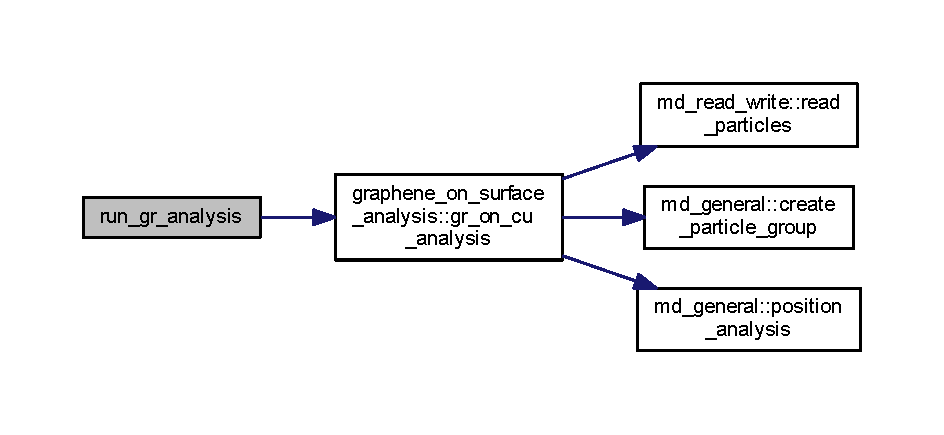
\includegraphics[width=350pt]{run__gr__analysis_8f90_a0eca5243bc06f4270ed032524f69b5ea_cgraph}
\end{center}
\end{figure}

\hypertarget{run__gr__moire__fitting_8f90}{}\section{Файл runners/run\+\_\+gr\+\_\+moire\+\_\+fitting.f90}
\label{run__gr__moire__fitting_8f90}\index{runners/run\+\_\+gr\+\_\+moire\+\_\+fitting.\+f90@{runners/run\+\_\+gr\+\_\+moire\+\_\+fitting.\+f90}}
\subsection*{Функции/подпрограммы}
\begin{DoxyCompactItemize}
\item 
program \mbox{\hyperlink{run__gr__moire__fitting_8f90_a3f54721279f970a03ea533479dbc2bd1}{run\+\_\+gr\+\_\+moire\+\_\+fitting}}
\item 
real function \mbox{\hyperlink{run__gr__moire__fitting_8f90_ab2a5771666cbc7ef9aff145187640f68}{delta\+\_\+error}} (error\+\_\+array)
\end{DoxyCompactItemize}


\subsection{Функции/подпрограммы}
\mbox{\Hypertarget{run__gr__moire__fitting_8f90_ab2a5771666cbc7ef9aff145187640f68}\label{run__gr__moire__fitting_8f90_ab2a5771666cbc7ef9aff145187640f68}} 
\index{run\+\_\+gr\+\_\+moire\+\_\+fitting.\+f90@{run\+\_\+gr\+\_\+moire\+\_\+fitting.\+f90}!delta\+\_\+error@{delta\+\_\+error}}
\index{delta\+\_\+error@{delta\+\_\+error}!run\+\_\+gr\+\_\+moire\+\_\+fitting.\+f90@{run\+\_\+gr\+\_\+moire\+\_\+fitting.\+f90}}
\subsubsection{\texorpdfstring{delta\+\_\+error()}{delta\_error()}}
{\footnotesize\ttfamily real function delta\+\_\+error (\begin{DoxyParamCaption}\item[{real, dimension(4)}]{error\+\_\+array }\end{DoxyParamCaption})}



См. определение в файле run\+\_\+gr\+\_\+moire\+\_\+fitting.\+f90 строка 108


\begin{DoxyCode}
108     \textcolor{keywordtype}{real}:: delta\_error,error\_array(4)
109     \mbox{\hyperlink{run__gr__moire__fitting_8f90_ab2a5771666cbc7ef9aff145187640f68}{delta\_error}} = maxval(error\_array)-minval(error\_array)
110     \textcolor{keywordflow}{return}
\end{DoxyCode}
\mbox{\Hypertarget{run__gr__moire__fitting_8f90_a3f54721279f970a03ea533479dbc2bd1}\label{run__gr__moire__fitting_8f90_a3f54721279f970a03ea533479dbc2bd1}} 
\index{run\+\_\+gr\+\_\+moire\+\_\+fitting.\+f90@{run\+\_\+gr\+\_\+moire\+\_\+fitting.\+f90}!run\+\_\+gr\+\_\+moire\+\_\+fitting@{run\+\_\+gr\+\_\+moire\+\_\+fitting}}
\index{run\+\_\+gr\+\_\+moire\+\_\+fitting@{run\+\_\+gr\+\_\+moire\+\_\+fitting}!run\+\_\+gr\+\_\+moire\+\_\+fitting.\+f90@{run\+\_\+gr\+\_\+moire\+\_\+fitting.\+f90}}
\subsubsection{\texorpdfstring{run\+\_\+gr\+\_\+moire\+\_\+fitting()}{run\_gr\_moire\_fitting()}}
{\footnotesize\ttfamily program run\+\_\+gr\+\_\+moire\+\_\+fitting (\begin{DoxyParamCaption}{ }\end{DoxyParamCaption})}



См. определение в файле run\+\_\+gr\+\_\+moire\+\_\+fitting.\+f90 строка 1

Граф вызовов\+:\nopagebreak
\begin{figure}[H]
\begin{center}
\leavevmode
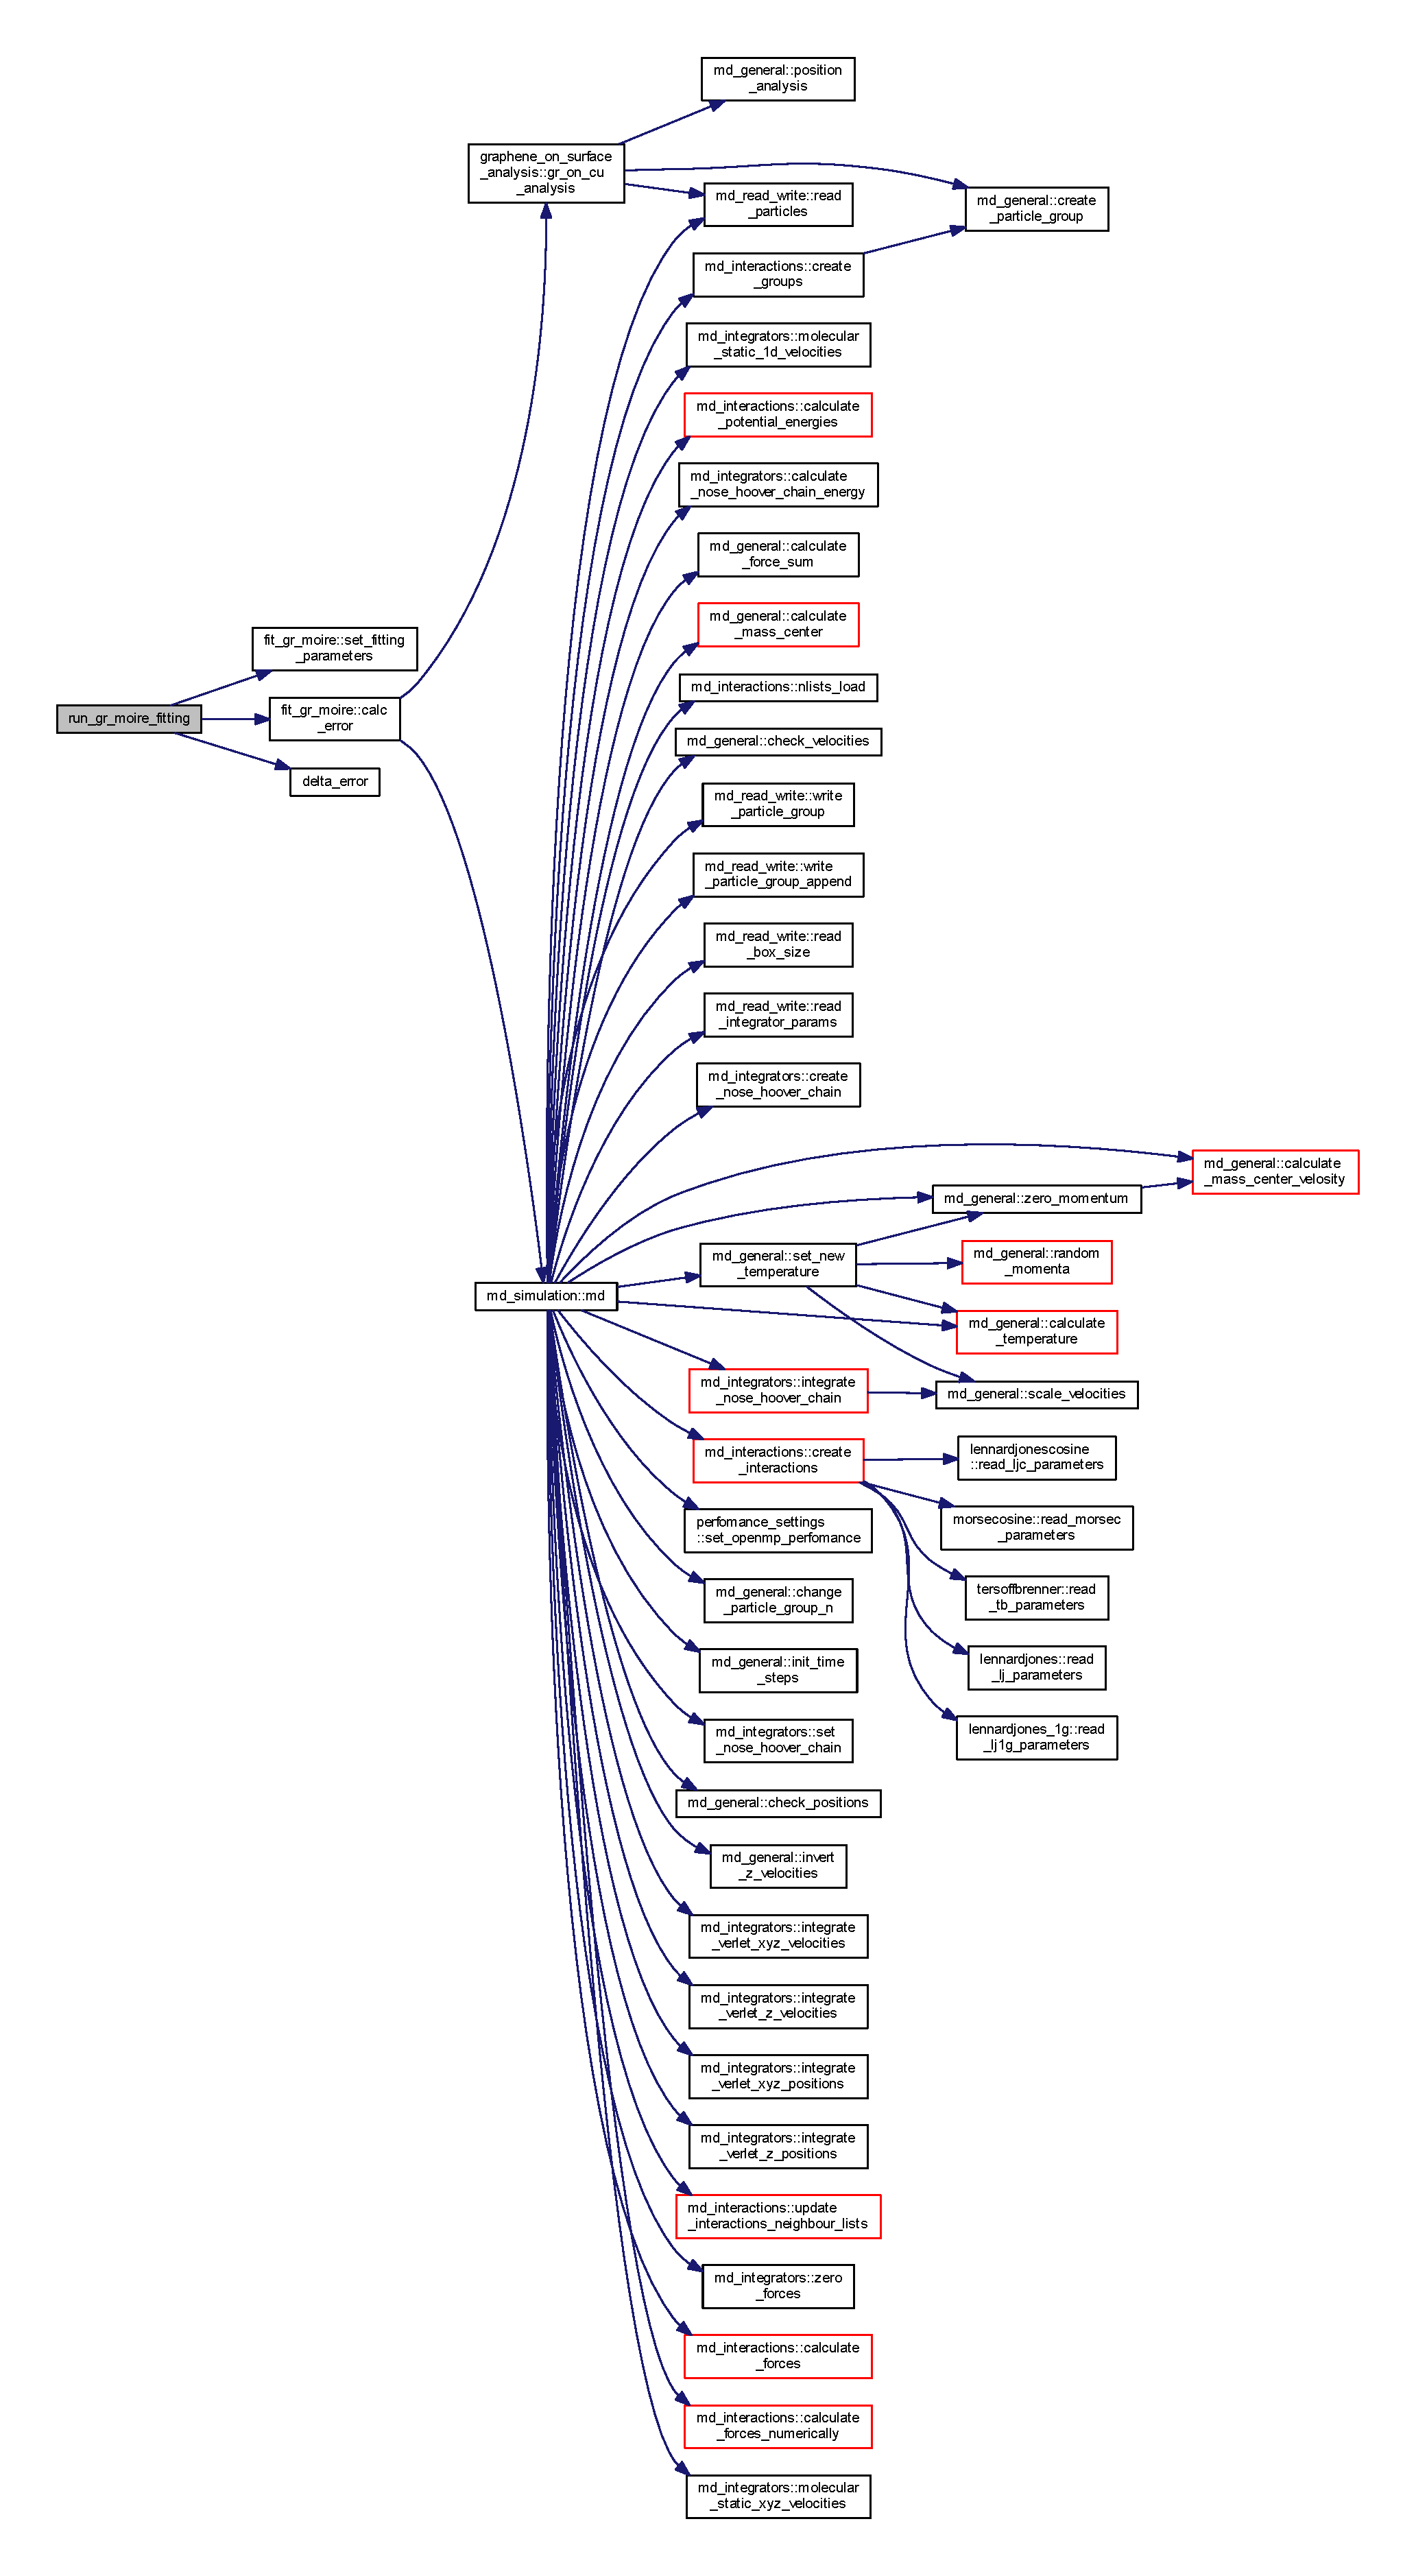
\includegraphics[height=550pt]{run__gr__moire__fitting_8f90_a3f54721279f970a03ea533479dbc2bd1_cgraph}
\end{center}
\end{figure}

\hypertarget{run__md__simulation_8f90}{}\section{Файл runners/run\+\_\+md\+\_\+simulation.f90}
\label{run__md__simulation_8f90}\index{runners/run\+\_\+md\+\_\+simulation.\+f90@{runners/run\+\_\+md\+\_\+simulation.\+f90}}
\subsection*{Функции/подпрограммы}
\begin{DoxyCompactItemize}
\item 
program \mbox{\hyperlink{run__md__simulation_8f90_a046456b29e3157bccd7d9d4e3c5f6b43}{md\+\_\+run}}
\end{DoxyCompactItemize}


\subsection{Функции/подпрограммы}
\mbox{\Hypertarget{run__md__simulation_8f90_a046456b29e3157bccd7d9d4e3c5f6b43}\label{run__md__simulation_8f90_a046456b29e3157bccd7d9d4e3c5f6b43}} 
\index{run\+\_\+md\+\_\+simulation.\+f90@{run\+\_\+md\+\_\+simulation.\+f90}!md\+\_\+run@{md\+\_\+run}}
\index{md\+\_\+run@{md\+\_\+run}!run\+\_\+md\+\_\+simulation.\+f90@{run\+\_\+md\+\_\+simulation.\+f90}}
\subsubsection{\texorpdfstring{md\+\_\+run()}{md\_run()}}
{\footnotesize\ttfamily program md\+\_\+run (\begin{DoxyParamCaption}{ }\end{DoxyParamCaption})}



См. определение в файле run\+\_\+md\+\_\+simulation.\+f90 строка 1

Граф вызовов\+:\nopagebreak
\begin{figure}[H]
\begin{center}
\leavevmode
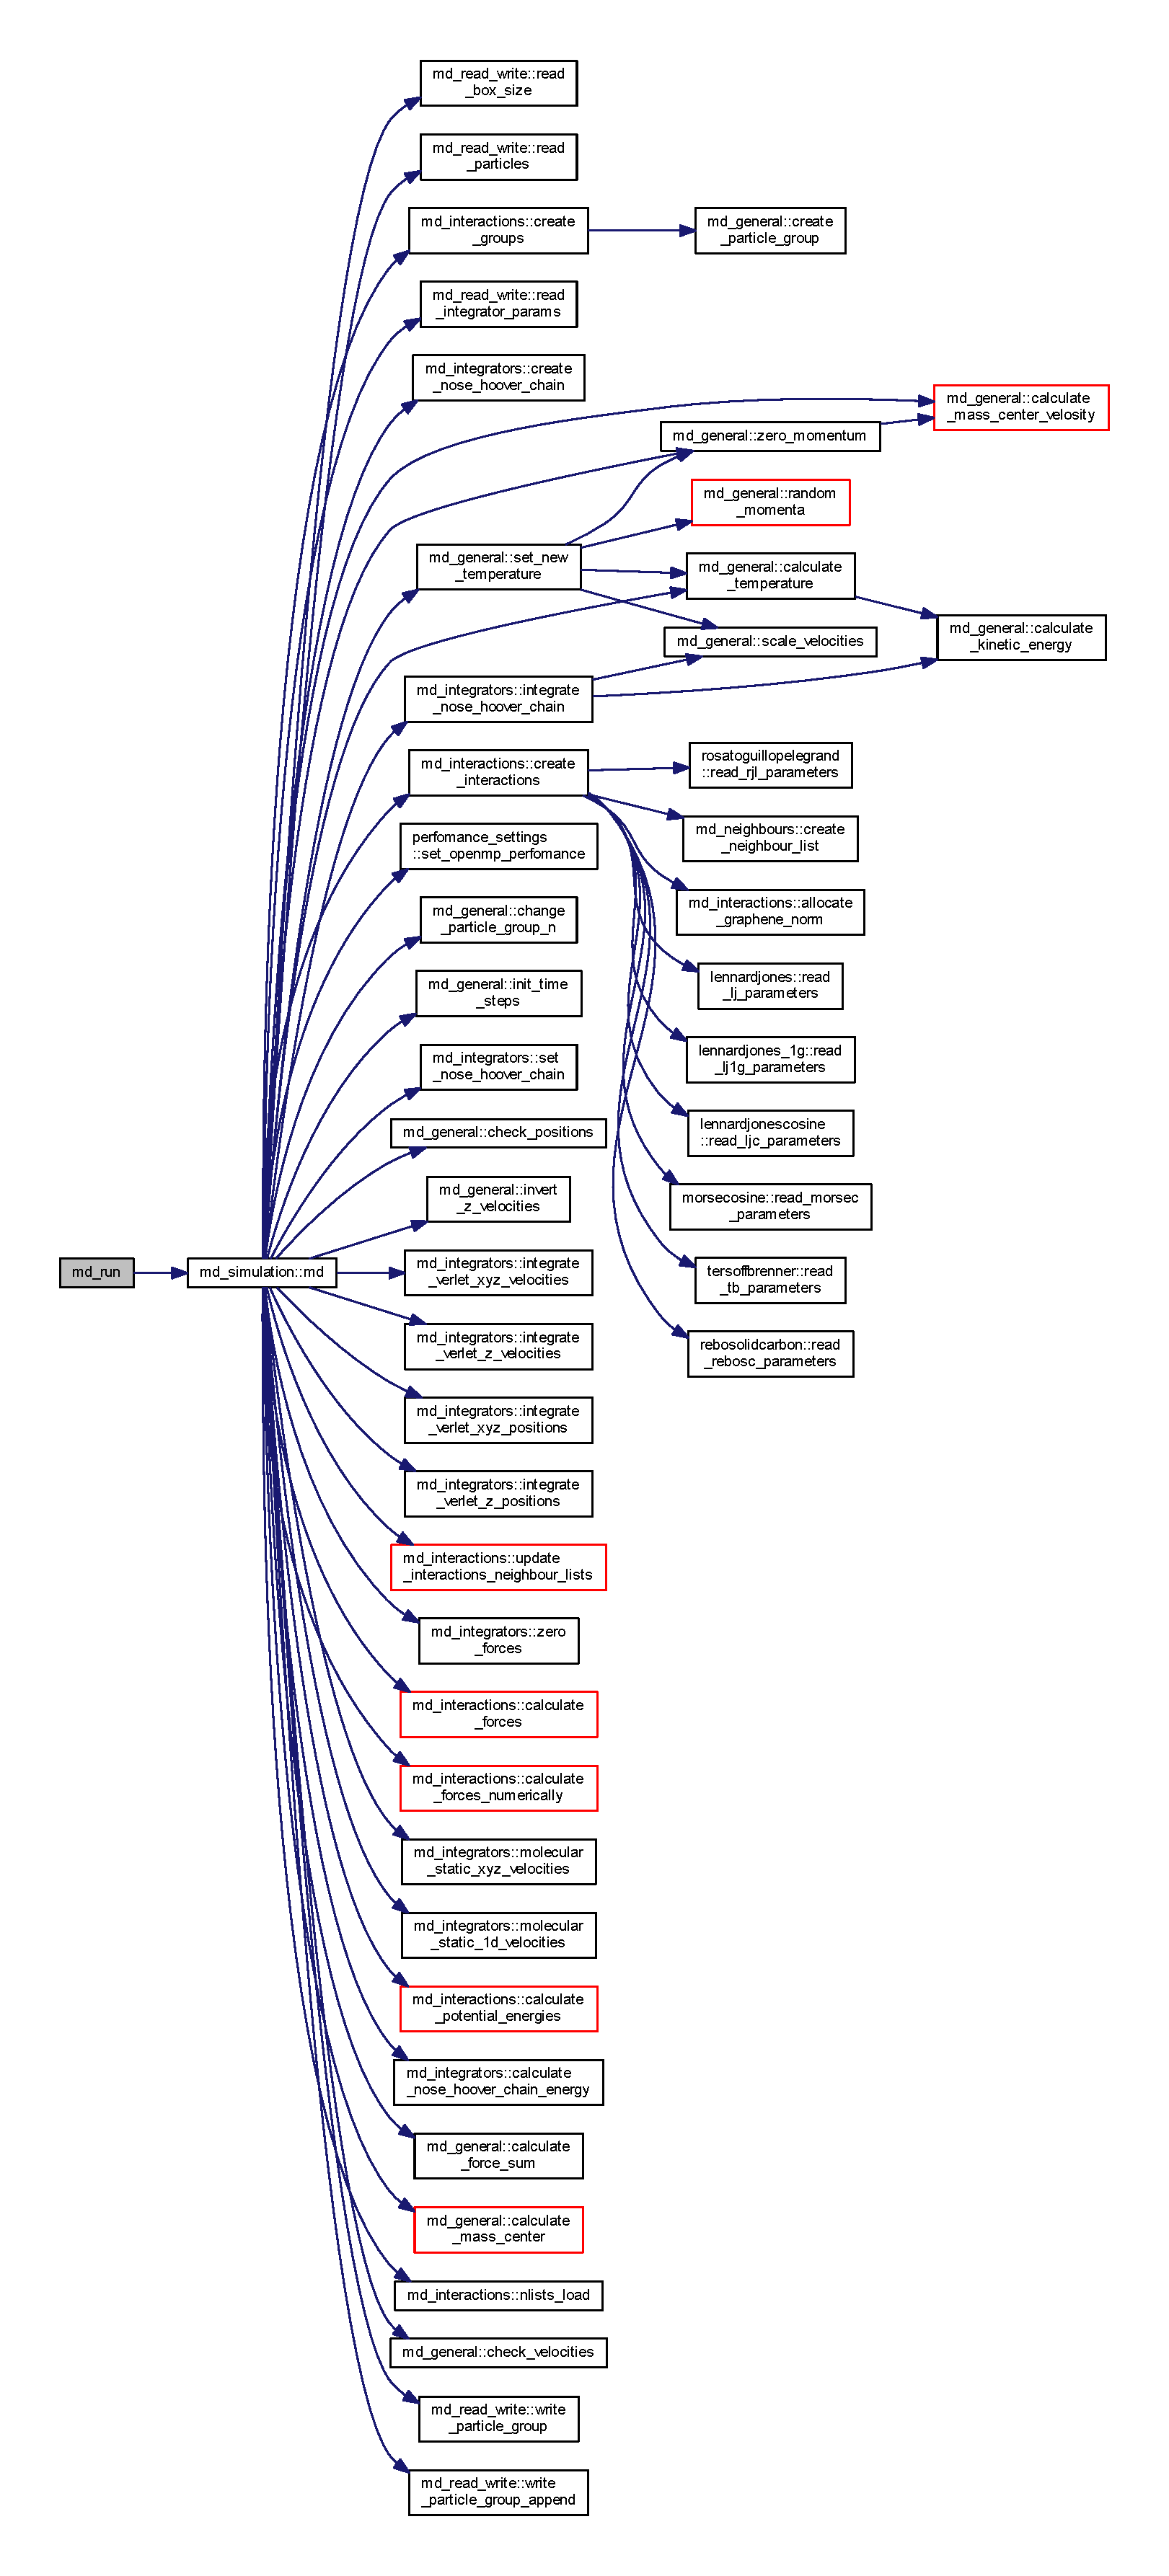
\includegraphics[height=550pt]{run__md__simulation_8f90_a046456b29e3157bccd7d9d4e3c5f6b43_cgraph}
\end{center}
\end{figure}

%--- End generated contents ---

% Index
\backmatter
\newpage
\phantomsection
\clearemptydoublepage
\addcontentsline{toc}{chapter}{Алфавитный указатель}
\printindex

\end{document}
